\documentclass[11pt,oneside]{book}
% ---------------------------------------------------------------------------
% Layout modelled on Murphy, "Machine Learning: A Probabilistic Perspective":
% a large chapter number with an italic title, section numbers hanging in the
% left margin, bold key terms, numbered equations, numbered theorems and
% algorithms, captions that name the script which drew each figure, footnotes
% for asides, and exercises at the end of each chapter.
% ---------------------------------------------------------------------------
\usepackage[paperwidth=7.5in, paperheight=10in, left=1.45in, right=0.85in,
            top=0.95in, bottom=0.95in, headsep=0.3in]{geometry}
\usepackage[T1]{fontenc}
\usepackage[utf8]{inputenc}
\usepackage[sc]{mathpazo}
\linespread{1.06}
\usepackage[scaled=0.88]{helvet}
\usepackage[varqu,scaled=0.95]{zi4}
\usepackage{microtype}
\usepackage{amsmath,amssymb,bm}
\usepackage{amsthm}
\usepackage{graphicx}
\usepackage{booktabs,array,multirow,tabularx,longtable}
\usepackage{xcolor}
\usepackage{enumitem}
\usepackage{caption}
\usepackage{subcaption}
\usepackage{titlesec}
\usepackage{fancyhdr}
\usepackage{listings}
\usepackage{tikz}
\usetikzlibrary{positioning,arrows.meta,fit,calc,shapes.geometric,shapes.misc,backgrounds,
                decorations.pathreplacing,patterns,matrix}
\usepackage{placeins}
\usepackage[hidelinks]{hyperref}
\usepackage{natbib}
\setcitestyle{authoryear,round}

% ---- palette (dataviz reference palette, light mode; text stays in ink) ----
\definecolor{vizblue}{HTML}{2A78D6}
\definecolor{vizorange}{HTML}{EB6834}
\definecolor{vizaqua}{HTML}{1BAF7A}
\definecolor{vizyellow}{HTML}{EDA100}
\definecolor{vizmagenta}{HTML}{E87BA4}
\definecolor{vizgreen}{HTML}{008300}
\definecolor{vizviolet}{HTML}{4A3AA7}
\definecolor{vizred}{HTML}{E34948}
\definecolor{inkprimary}{HTML}{0B0B0B}
\definecolor{inksecondary}{HTML}{52514E}
\definecolor{inkmuted}{HTML}{898781}
\definecolor{gridline}{HTML}{E1E0D9}
\definecolor{codeback}{HTML}{F6F5F2}

% ---- chapter and section headings (numbers hang in the margin) ----
\titleformat{\chapter}[display]
  {\normalfont\raggedright}
  {\fontsize{64}{64}\selectfont\bfseries\color{inkprimary}\thechapter}
  {6pt}
  {\Huge\itshape}
  [\vspace{2pt}]
\titleformat{name=\chapter,numberless}[display]
  {\normalfont\raggedright}{}{0pt}{\Huge\itshape}
\titlespacing*{\chapter}{0pt}{0.2in}{0.45in}
\titleformat{\section}{\normalfont\Large\bfseries}{\llap{\thesection\hspace{1.1em}}}{0pt}{}
\titleformat{\subsection}{\normalfont\large\bfseries}{\llap{\thesubsection\hspace{1.1em}}}{0pt}{}
\titleformat{\subsubsection}{\normalfont\normalsize\bfseries}{\llap{\thesubsubsection\hspace{1.1em}}}{0pt}{}
\titlespacing*{\section}{0pt}{3.2ex plus 1ex minus .2ex}{1.4ex plus .2ex}
\titlespacing*{\subsection}{0pt}{2.6ex plus 1ex minus .2ex}{1.1ex plus .2ex}
\titlespacing*{\subsubsection}{0pt}{2.2ex plus 1ex minus .2ex}{0.9ex plus .2ex}
\setcounter{secnumdepth}{3}
\setcounter{tocdepth}{1}

% ---- running heads: page number, then "Chapter N. Title" in italics ----
\pagestyle{fancy}
\fancyhf{}
\renewcommand{\headrulewidth}{0pt}
\makeatletter
\renewcommand{\chaptermark}[1]{\markboth{\ifnum\value{chapter}>0 \@chapapp\ \thechapter. \fi #1}{}}
\makeatother
\fancyhead[L]{\small\thepage}
\fancyhead[R]{\small\itshape\nouppercase{\leftmark}}
\fancypagestyle{plain}{\fancyhf{}\fancyfoot[C]{\small\thepage}}

% ---- captions: bold label, small text; each ends with its generating script ----
% Captions end in file paths, so they may use loose lines rather than run into the margin.
\DeclareCaptionFont{sloppy}{\sloppy}
\captionsetup{font={small,sloppy}, labelfont=bf, labelsep=colon, justification=justified,
              singlelinecheck=false, skip=6pt}
\newcommand{\generatedby}[1]{Figure generated by \file{#1}.}
\newcommand{\drawnin}[1]{Diagram drawn in \file{#1}.}

% ---- vocabulary ----
\newcommand{\keyterm}[1]{\textbf{#1}}
% File paths in typewriter type, breakable after "/" and "_" so long paths never overflow.
\ExplSyntaxOn
\tl_new:N \l__sol_path_tl
\NewDocumentCommand \file { m }
  {
    \tl_set:Nn \l__sol_path_tl {#1}
    \tl_replace_all:Nnn \l__sol_path_tl { / } { / \allowbreak }
    \tl_replace_all:Nnn \l__sol_path_tl { \_ } { \_ \allowbreak }
    \texttt { \upshape \l__sol_path_tl }
  }
\ExplSyntaxOff
% A third line-breaking pass with extra stretch before any line is allowed to overflow.
\setlength{\emergencystretch}{3em}
\newcommand{\Ha}{H$\alpha$}
\newcommand{\PQ}{\mathrm{PQ}}
\newcommand{\SQ}{\mathrm{SQ}}
\newcommand{\RQ}{\mathrm{RQ}}
\newcommand{\IoU}{\mathrm{IoU}}
\newcommand{\TP}{\mathrm{TP}}
\newcommand{\FP}{\mathrm{FP}}
\newcommand{\FN}{\mathrm{FN}}
\newcommand{\R}{\mathbb{R}}
\newcommand{\E}{\mathbb{E}}
\newcommand{\argmin}{\operatorname*{arg\,min}}
\newcommand{\argmax}{\operatorname*{arg\,max}}
\newcommand{\sigmoid}{\sigma}
\newcommand{\softmax}{\operatorname{softmax}}

% ---- code listings ----
\lstdefinestyle{repo}{
  language=Python,
  basicstyle=\ttfamily\footnotesize,
  keywordstyle=\color{vizblue}\bfseries,
  commentstyle=\color{inkmuted},
  stringstyle=\color{vizorange!85!black},
  numberstyle=\tiny\color{inkmuted},
  numbers=left, numbersep=10pt,
  backgroundcolor=\color{codeback},
  frame=l, framerule=1.2pt, rulecolor=\color{vizblue!45},
  xleftmargin=20pt, framexleftmargin=4pt,
  showstringspaces=false, breaklines=true, breakatwhitespace=true,
  columns=fullflexible, keepspaces=true, tabsize=4,
  aboveskip=8pt, belowskip=6pt,
  % Listings are kept to ASCII: pdflatex's listings cannot typeset multi-byte UTF-8.
}
\lstset{style=repo}
\renewcommand{\lstlistingname}{Listing}
\captionsetup[lstlisting]{font=small, labelfont=bf, skip=4pt, justification=raggedright,
                           singlelinecheck=false}

% ---- theorems, as in Murphy: numbered within the chapter ----
\theoremstyle{plain}
\newtheorem{theorem}{Theorem}[chapter]
\newtheorem{proposition}[theorem]{Proposition}
\theoremstyle{definition}
\newtheorem{definition}[theorem]{Definition}

% ---- algorithms, as in Murphy: a ruled block with numbered lines ----
% Usage: \begin{algorithmblock}{title} \item first line \item \Ind indented line \end{algorithmblock}
\newcounter{algorithmblock}[chapter]
\renewcommand{\thealgorithmblock}{\thechapter.\arabic{algorithmblock}}
\def\theHalgorithmblock{\thechapter.\arabic{algorithmblock}}   % unique hyperref anchors
\newcommand{\Ind}{\hspace*{1.4em}}
\newenvironment{algorithmblock}[1]{%
  \par\medskip\refstepcounter{algorithmblock}%
  \noindent\rule{\linewidth}{0.7pt}\par\nopagebreak\vspace{0.3ex}%
  \noindent{\small\textbf{Algorithm \thealgorithmblock:}\ #1}\par\nopagebreak\vspace{-0.4ex}%
  \noindent\rule{\linewidth}{0.4pt}\par\nopagebreak\vspace{-0.6ex}%
  \small
  \begin{enumerate}[label={\color{inkmuted}\scriptsize\arabic*}, leftmargin=2.2em, labelsep=0.9em,
                    itemsep=0.5pt, parsep=0pt, topsep=3pt]}%
  {\end{enumerate}\vspace{-0.6ex}\noindent\rule{\linewidth}{0.7pt}\par\medskip}

% ---- epigraph under a chapter's first section, as in Murphy ----
\newcommand{\epigraph}[2]{\begin{quote}\small\itshape #1\par\nopagebreak\vspace{0.3ex}
  {\raggedleft\upshape--- #2\par}\end{quote}\vspace{0.5ex}}

% ---- exercises, as in Murphy: "Exercise N.M Title", optional source line ----
\newcounter{exercise}[chapter]
\renewcommand{\theexercise}{\thechapter.\arabic{exercise}}
\def\theHexercise{\thechapter.\arabic{exercise}}   % unique hyperref anchors
\newenvironment{exercise}[2][]{%
  \par\medskip\refstepcounter{exercise}\noindent\textbf{Exercise \theexercise}\ \ #2%
  \ifx\relax#1\relax\else\par\noindent{\small(Source: #1.)}\fi\par\smallskip\noindent\ignorespaces}%
  {\par\medskip}

% ---- TikZ styles shared by the diagrams ----
\tikzset{
  >={Stealth[length=2.2mm]},
  box/.style={draw=#1, line width=0.8pt, fill=#1!9, rounded corners=2.5pt, align=center,
              inner sep=4pt, font=\sffamily\footnotesize, text=inksecondary},
  box/.default=inkmuted,
  flow/.style={->, line width=0.8pt, draw=inksecondary},
  dashflow/.style={->, line width=0.7pt, draw=inkmuted, dashed},
  note/.style={font=\sffamily\scriptsize, text=inksecondary, align=center},
  title/.style={font=\sffamily\footnotesize\bfseries, text=inkprimary},
}

\hypersetup{colorlinks=true, linkcolor=vizblue!80!black, citecolor=vizblue!80!black,
            urlcolor=vizblue!80!black}

% Generated by paper/make_figures.py from measured JSON. Do not edit by hand.
\newcommand{\HostPQ}{0.4705}
\newcommand{\OurPQ}{0.4705}
\newcommand{\NumTP}{881}
\newcommand{\NumFP}{361}
\newcommand{\NumFN}{444}
\newcommand{\ValSQ}{0.685}
\newcommand{\ValRQ}{0.686}
\newcommand{\MeanIoUOverlap}{0.605}
\newcommand{\MeanDiceOverlap}{0.734}
\newcommand{\ValPhotos}{106}
\newcommand{\ValRecords}{180}
\newcommand{\ValGT}{1325}
\newcommand{\ValPred}{756}
\newcommand{\GTMissedPct}{18.5}
\newcommand{\GTOneOnePct}{78.7}
\newcommand{\GTSplitPct}{2.8}
\newcommand{\PredUnmatchedPct}{13.3}
\newcommand{\PredOneOnePct}{83.5}
\newcommand{\PredMergePct}{3.2}
\newcommand{\HumanPQ}{0.347}
\newcommand{\HumanPQAll}{0.340}
\newcommand{\HumanPairs}{1196}
\newcommand{\HumanValPairs}{202}
\newcommand{\HumanSQ}{0.636}
\newcommand{\HumanRQ}{0.546}
\newcommand{\SecondsPerPhoto}{2.49}
\newcommand{\InferenceGPU}{T4}
\newcommand{\TestMinutes}{7}
\newcommand{\PeakGiB}{2.7}
\newcommand{\LoadSeconds}{1.4}
\newcommand{\EpochFortyPQ}{0.4680}
\newcommand{\EpochFiftyPQ}{0.4636}
\newcommand{\BestEpoch}{40}
\newcommand{\RecallSmall}{0.45}
\newcommand{\RecallLarge}{0.75}
\newcommand{\PrecisionSmall}{0.55}
\newcommand{\PrecisionLarge}{0.82}
\newcommand{\SmallArea}{471}
\newcommand{\LargeArea}{3183}
\newcommand{\QualPQ}{0.478}
\newcommand{\QualMedian}{0.479}
\newcommand{\QualCandidates}{34}
\newcommand{\Submissions}{31}
\newcommand{\FirstPublic}{0.26}
\newcommand{\BestPublic}{0.41}
\newcommand{\FloatFortyPQ}{0.4705}
\newcommand{\FloatFiftyPQ}{0.4621}
\newcommand{\SoupPQ}{0.4688}
\newcommand{\FusionPQ}{0.4700}
\newcommand{\FusionExtraTP}{60}
\newcommand{\FusionExtraFP}{125}
\newcommand{\FailMissArea}{644}
\newcommand{\FailFPArea}{813}
\newcommand{\FailSplitArea}{14568}
\newcommand{\PQLow}{0.450}
\newcommand{\PQHigh}{0.491}
\newcommand{\SQLow}{0.680}
\newcommand{\SQHigh}{0.691}
\newcommand{\RQLow}{0.657}
\newcommand{\RQHigh}{0.715}
\newcommand{\HumanPQLow}{0.314}
\newcommand{\HumanPQHigh}{0.383}
\newcommand{\HumanPhotos}{47}
\newcommand{\RecallSmallLow}{0.39}
\newcommand{\RecallSmallHigh}{0.52}
\newcommand{\RecallLargeLow}{0.69}
\newcommand{\RecallLargeHigh}{0.80}
\newcommand{\PerBin}{221}
\newcommand{\AllPhotos}{707}
\newcommand{\AllRecords}{1154}
\newcommand{\AllFilaments}{8199}
\newcommand{\TrainPhotos}{601}
\newcommand{\TrainRecords}{974}
\newcommand{\TrainGT}{6874}

% Generated by book/make_book_figures.py from measured JSON. Do not edit by hand.
\newcommand{\LongPfifty}{96}
\newcommand{\LongPninety}{233}
\newcommand{\LongPninetynine}{509}
\newcommand{\LongMax}{1067}
\newcommand{\AreaMedian}{1228}
\newcommand{\AreaPten}{410}
\newcommand{\MaxPerRecord}{26}
\newcommand{\MeanPerRecord}{7.1}
\newcommand{\EmptyRecords}{0}
\newcommand{\OnceAnnotated}{411}
\newcommand{\TwiceAnnotated}{145}
\newcommand{\ThriceAnnotated}{151}
\newcommand{\TestPhotos}{180}
\newcommand{\StationBh}{118}
\newcommand{\StationCh}{125}
\newcommand{\StationLh}{127}
\newcommand{\StationMh}{125}
\newcommand{\StationTh}{110}
\newcommand{\StationUh}{102}
\newcommand{\RasterCoco}{339}
\newcommand{\RasterCv}{386}
\newcommand{\RasterRatio}{1.14}
\newcommand{\RasterIoU}{0.869}
\newcommand{\AnnotatorOne}{18}
\newcommand{\AnnotatorTwo}{22}
\newcommand{\AnnotatorThree}{18}
\newcommand{\LeverageRecover}{0.4864}
\newcommand{\LeverageRemove}{0.4799}
\newcommand{\LeveragePolish}{0.4725}
\newcommand{\ValPublicPoints}{16}


\begin{document}
\frontmatter

\begin{titlepage}
\centering
\vspace*{1.2in}
{\fontsize{34}{40}\selectfont\itshape Finding Filaments\par}
\vspace{0.25in}
{\Large Instance segmentation of solar filaments\\ in full-disk \Ha{} images\par}
\vspace{0.5in}
{\large A documented pipeline, the pitfalls along the way,\\ and the experiments that did not work\par}
\vfill
\begin{tikzpicture}
  \foreach \c/\x in {vizblue/0, vizorange/0.55, vizaqua/1.1, vizviolet/1.65, vizyellow/2.2}
    \fill[\c] (\x,0) rectangle ++(0.45,0.08);
\end{tikzpicture}
\par\vspace{0.3in}
{\large Written for Kasozi Ismail\par}
\vspace{0.12in}
{\normalsize Kaggle team \texttt{supersede}\par}
\vspace{0.04in}
{\normalsize\href{mailto:k.kasozi69@gmail.com}{\texttt{k.kasozi69@gmail.com}}\par}
\vspace{0.2in}
{\normalsize September 2026\par}
\vspace*{0.4in}
\end{titlepage}

\chapter*{Preface}
\markboth{Preface}{}
\addcontentsline{toc}{chapter}{Preface}

\section*{Introduction}
Solar filaments are the long, dark structures that cross the disk of the Sun when it is
photographed in the red \Ha{} line of hydrogen. Each one is a cloud of cool, dense plasma held up
by the Sun's magnetic field, and its eruption can be accompanied by a coronal mass ejection.
Catalogues of filaments are therefore useful for studying the solar cycle and for forecasting
space weather, but drawing them by hand is slow. The Solar Filament Segmentation Challenge 2026, a
Kaggle competition, asked for a program that finds every filament in a full-disk \Ha{} image from
the Global Oscillation Network Group (GONG) and outlines each one as a separate mask.

This book is a detailed account of one entry to that challenge. It is written for readers who
want to build on the work: solar physicists who need filament masks, and machine-learning
practitioners who want to apply instance segmentation to solar images. We think that three parts
of it are useful beyond the competition.
\begin{enumerate}[leftmargin=*,itemsep=2pt]
\item \textbf{A complete, documented pipeline.} The book follows every step from the annotation
file to a Mask2Former model that predicts at the native resolution of $2048\times2048$ pixels, and
from its predictions to the file that the competition scores. Each step is explained and tied to
the code that performs it.
\item \textbf{Pitfalls that carry over to other projects.} Two standard libraries turn the same
annotated polygon into masks of different sizes (Section~\ref{sec:masks-fat}). A validation split
that keeps each photograph on one side still leaks information, because a filament survives on the
disk for days (Section~\ref{sec:val-time}). And a transformer trained only on crops meets
unfamiliar positional embeddings when it is applied to a whole image
(Section~\ref{sec:train-sampling}). All three are easy to miss.
\item \textbf{Negative results.} Between 24 August and 21 September 2026 we ran more than 140
numbered experiments, and most of them did not improve the model. We describe them in some detail,
because the reasons they failed tell us a good deal about the data, the metric and the models, and
because an idea whose failure has been measured and written down need not be tried again.
\end{enumerate}
The final model reaches a panoptic quality of \HostPQ{} on our validation split and \BestPublic{}
on the competition's public leaderboard. We quote these numbers because the decisions in the book
rest on measurements of this kind. Chapter~\ref{ch:submission} discusses what they show and what
they do not, and Section~\ref{sec:intro-previous} explains why no published result can yet be
compared with them.

\section*{Target audience}
Most of the book assumes a reader who already knows the main families of image models. We
assume that you have trained a convolutional network, that you know roughly how YOLO and the
Vision Transformer (ViT) work, and that you can read Python and PyTorch. We do not assume any
knowledge of solar physics, of segmentation metrics, or of this repository. Chapter~\ref{ch:transformers}
reviews the transformer machinery that the final model uses (attention, Swin, DETR) from first
principles, so familiarity with it helps but is not required. Readers who want a fuller
introduction to deep learning can consult \citet{bishop}.

\section*{A measurement-driven approach}
Murphy's textbook~\citep{murphy}, whose layout this book borrows, argues for a principled, model-based approach
to machine learning in place of a cookbook of heuristics. The corresponding principle in this
book is that each design decision should rest on a measurement. Three kinds of measurement recur
throughout. The first is an exact reproduction of a baseline, made before any change is compared
with it. The second is an \emph{oracle}, which uses the ground truth to find the best score that
a whole family of methods could possibly reach; it tells us whether an idea is worth building
before we build it. The third is a short calculation, based on the structure of the metric, of
what a change must achieve before it can raise the score at all. We introduce these tools in
Chapters~\ref{ch:metric} and~\ref{ch:validation}, and we use them in most of the chapters that
follow.

\section*{A practical approach}
Nearly everything in this book is backed by code in the repository, and we refer to files by
their path, for example \file{shared/utils.py}. Every figure that shows data names the function
that drew it, in the form ``Figure generated by \file{book/make\_book\_figures.py:fig\_split}'',
so that you can regenerate the figure and modify it. Diagrams that do not come from data say
where they are drawn. When we quote a number from the history of the project, we name the
experiment that produced it, for example exp013. The full record of each experiment is kept in
\file{docs/ACTIVE\_EXPERIMENT.md} and \file{docs/leaderboard-analysis.md}, and
Appendix~\ref{app:ledger} lists all of them in order.

\section*{How the book is organised}
Chapter~\ref{ch:intro} gives an overview of the problem and of our results.
Chapters~\ref{ch:data}--\ref{ch:validation} lay the foundations: the Sun and the data
(Chapter~\ref{ch:data}), how masks are represented and compared (Chapter~\ref{ch:masks}), the
competition's metric (Chapter~\ref{ch:metric}), and how we validate models
(Chapter~\ref{ch:validation}). Chapters~\ref{ch:paradigms}--\ref{ch:recall} describe the
approaches we tried, in roughly the order in which we tried them: dense semantic segmentation
(Chapter~\ref{ch:paradigms}), YOLO instance segmentation (Chapter~\ref{ch:yolo}), test-time
augmentation and ensembles (Chapter~\ref{ch:tta}), correcting masks after prediction
(Chapter~\ref{ch:post}), and recovering the filaments that a detector misses
(Chapter~\ref{ch:recall}). Chapters~\ref{ch:transformers}--\ref{ch:submission} describe the
final model: the transformer architecture it is built on (Chapter~\ref{ch:transformers}), how
we trained it (Chapter~\ref{ch:training}), and how its predictions become a submission and how
good that submission is (Chapter~\ref{ch:submission}). Chapter~\ref{ch:lessons} collects what we
learned about experimental method, much of it from our own mistakes. The appendices describe the
computing infrastructure, list every experiment, give a map of the code and summarise the
notation.

\section*{Starred sections}
As in Murphy's book, a section whose title ends in an asterisk (*) contains detail that can be
skipped on a first reading without losing the thread of the chapter.

\section*{Exercises}
Each chapter ends with exercises. Most of them ask you to reproduce a number from the chapter,
to derive a result that the chapter used without proof, or to extend one of its analyses. Doing
a few of them is the quickest way to become familiar with the code and the data.

\section*{Scope}
The book describes the project as it stood on 21 September 2026. The competition closes on
15 November 2026, so later work will extend the story. One rule holds throughout: the public
MAGFiLO release contains the annotations of the competition's test photographs, and we never
train on it (Section~\ref{sec:data-rules} explains why).

\tableofcontents

\mainmatter
\chapter{Introduction}\label{ch:intro}

\section{Solar filament segmentation: what and why?}\label{sec:intro-what}
\epigraph{Nature uses only the longest threads to weave her patterns.}{Richard Feynman,
\emph{The Character of Physical Law} \citeyearpar{feynman1965}}

Photographed through a filter that passes only one red line of hydrogen, the Sun does not look
like a smooth bright ball. Its disk is covered with a mottled pattern of darker and brighter
cells, and across this pattern lie long, dark, thread-like structures called \keyterm{solar
filaments}. A filament is a cloud of cool, dense gas held up in the Sun's atmosphere by its
magnetic field~\citep{mackay2010,parenti2014}. Filaments can remain stable for days or weeks and
then erupt, and an eruption can be accompanied by a coronal mass ejection~\citep{webb2012}, a
cloud of magnetised plasma that may travel to the Earth.\footnote{A coronal mass ejection that reaches the Earth can disturb its magnetic field,
which in turn can affect satellites, radio communication and power grids.} Catalogues of filaments are therefore useful both to solar physicists and to
space-weather forecasters, and compiling them by hand is slow and tedious. This book is about a
machine-learning system that finds and outlines filaments automatically.

The precise task is set by a Kaggle competition, the Solar Filament Segmentation Challenge
2026~\citep{challenge}. The input is a single photograph of the Sun: a $2048\times2048$ grey
image taken through a filter that passes only the red \Ha{} line of hydrogen. The output is a
list of \keyterm{instance masks}, one binary image per filament, each marking the pixels that
belong to that filament, with the constraint that no pixel may belong to two masks. Each mask is
written as one row of a CSV file, in a compressed format called run-length encoding
(Section~\ref{sec:masks-rle}). A server compares these rows with masks drawn by human experts and
returns a single number between 0 and 1, the \keyterm{Panoptic Quality} (PQ), which we study in
Chapter~\ref{ch:metric}. Figure~\ref{fig:intro-task} summarises the setup. In the vocabulary of
computer vision, this is an \keyterm{instance segmentation} problem with a single object class;
we make the terminology precise in Section~\ref{sec:paradigms-kinds}.

\begin{figure}[t]
\centering
\begin{tikzpicture}[node distance=0.55cm]
  \node (in) {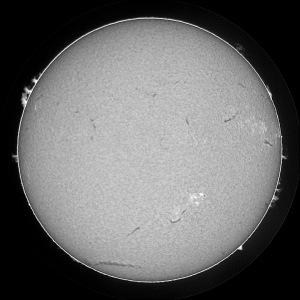
\includegraphics[width=2.1cm]{figures/thumb_input.png}};
  \node[note, below=0pt of in] {\Ha{} photograph\\ $2048\times2048$, grey};
  \node[box=vizblue, right=of in, minimum height=1.6cm, text width=2.3cm] (model)
       {\textbf{\color{inkprimary}segmentation model}\\[2pt] finds filaments and traces each one};
  \node[right=of model] (out) {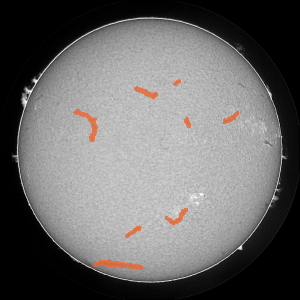
\includegraphics[width=2.1cm]{figures/thumb_output.png}};
  \node[note, below=0pt of out] {disjoint instance masks\\ (orange)};
  \node[box=vizorange, right=of out, minimum height=1.6cm, text width=2.0cm] (csv)
       {\textbf{\color{inkprimary}CSV}\\[2pt] one RLE row per filament};
  \draw[flow] (in) -- (model); \draw[flow] (model) -- (out); \draw[flow] (out) -- (csv);
  \node[box=vizaqua, below=1.25cm of csv, text width=2.0cm] (score) {\textbf{\color{inkprimary}PQ}\\ vs.\ each annotator};
  \draw[flow] (csv) -- (score);
\end{tikzpicture}
\caption{The task. A model turns one \Ha{} photograph into a set of non-overlapping masks, one per
filament. The masks are encoded as rows of a CSV file and scored with Panoptic Quality against
every annotator who labelled that photograph. \drawnin{book/chapters/ch01\_introduction.tex}}
\label{fig:intro-task}
\end{figure}

\subsection{Three questions in one}\label{sec:intro-questions}
It helps to recognise that the task combines three different questions.
\begin{enumerate}[leftmargin=*,itemsep=2pt]
\item \keyterm{Detection}: is there a filament at this location at all?
\item \keyterm{Delineation}: which pixels belong to it?
\item \keyterm{Identity}: is this dark region one filament, or two filaments that happen to
touch?
\end{enumerate}
A method can answer one of these questions well and another poorly. For example, the semantic
segmentation models of Chapter~\ref{ch:paradigms} delineate filaments reasonably well but have
no good way to decide identity; the YOLO models of Chapter~\ref{ch:yolo} detect filaments well
but draw masks that are slightly too wide; and the Mask2Former model of
Chapters~\ref{ch:transformers}--\ref{ch:submission} handles identity best of all but still misses
many faint filaments. The metric folds all three questions into one number, so a change in the
score seldom tells us, on its own, which of the three a change has improved. For this reason we
will often split the score into its parts (Section~\ref{sec:metric-sqrq}).

\section{Why the problem is hard}\label{sec:intro-hard}
Several properties of filaments make them difficult to segment. First, they are thin. The median
filament's bounding box is \LongPfifty{} pixels on its long side at the native resolution, but
its body is often only four or five pixels wide, so any step that reduces the resolution of the
image risks erasing it. Second, they are dark, but so is much else on the disk. The chromosphere
is covered by a network of dark and bright cells, and, pixel by pixel, a filament is no darker
than the network that surrounds it (we measure this in Section~\ref{sec:recall-physics}). Third,
they fade gradually into their surroundings, so where a filament ends is a matter of judgement,
and the image shows no sharp edge there. Fourth, a filament is often broken into several dark
patches that the eye groups into one object. Finally, near the edge of the disk (the
\keyterm{limb}), where the surface of the Sun curves away from us, filaments appear foreshortened
and dimmer.

The labels inherit all of these difficulties. Figure~\ref{fig:intro-annotators} shows one
photograph that three experts annotated independently. They agree about the large filaments, but
they draw \AnnotatorOne{}, \AnnotatorTwo{} and \AnnotatorThree{} filaments respectively, they
split and merge structures differently, and their outlines of the same filament differ by several
pixels. If we score one expert's masks against another expert's masks with the competition's
metric, we obtain a PQ of only about \HumanPQAll{} (Section~\ref{sec:metric-agreement}). This
fact shapes much of what follows: the target we are asked to predict is one person's judgement,
and different people judge differently. It does \emph{not} follow that \HumanPQAll{} is an upper
limit on what a model can score, and Section~\ref{sec:metric-agreement} explains why.

\begin{figure}[t]
\centering
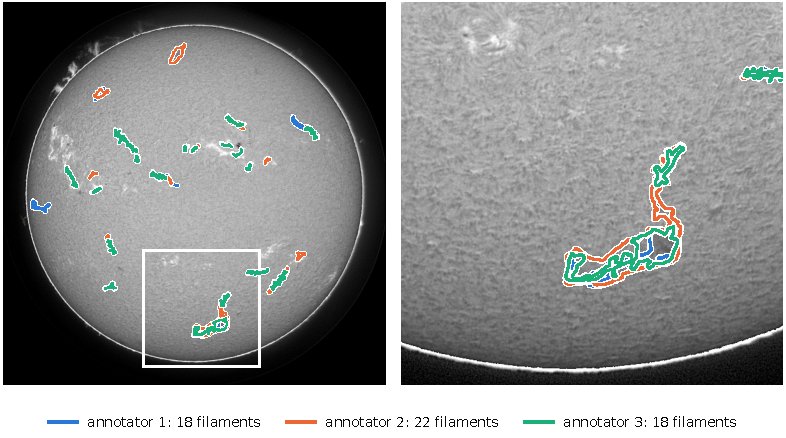
\includegraphics[width=\textwidth]{figures/fig_annotators.pdf}
\caption{One photograph labelled by three annotators working independently. Left: the full disk
with every annotator's outlines; the box marks the region shown on the right. Right: a
native-resolution zoom. The annotators agree that a filament is present, but not about its
extent or about how many pieces it consists of.
\generatedby{book/make\_book\_figures.py:fig\_annotators}}
\label{fig:intro-annotators}
\end{figure}

\section{The data}\label{sec:intro-data}
The competition supplies \AllPhotos{} training photographs with \AllRecords{} annotation
\keyterm{records}, where a record is one annotator's complete labelling of one photograph. Most
photographs were labelled once, but \TwiceAnnotated{} were labelled twice and \ThriceAnnotated{}
three times, which is why there are more records than photographs. In total the records contain
\AllFilaments{} annotated filaments. Each filament is stored as a polygon together with a traced
centre line called its \keyterm{spine}. The test set contains \TestPhotos{} photographs whose
labels are hidden. The public leaderboard scores roughly half of them, and the other half are
kept for the final ranking. Chapter~\ref{ch:data} describes the data in detail.

\section{The metric}\label{sec:intro-metric}
Panoptic Quality compares the predicted masks with the masks of one annotator at a time. A
predicted mask and an annotated mask \keyterm{match} if their intersection over union (IoU)
exceeds 0.5. Matched pairs are called \keyterm{true positives} (TP), unmatched predictions are
\keyterm{false positives} (FP), and unmatched annotations are \keyterm{false negatives} (FN).
The score is
\begin{equation}
\PQ = \frac{\sum_{(p,g)\in\TP}\IoU(p,g)}{|\TP| + \tfrac12|\FP| + \tfrac12|\FN|}
    = \underbrace{\frac{\sum_{\TP}\IoU}{|\TP|}}_{\SQ}\times
      \underbrace{\frac{|\TP|}{|\TP| + \tfrac12|\FP| + \tfrac12|\FN|}}_{\RQ},
\label{eq:intro-pq}
\end{equation}
where the counts are pooled over all annotation records. The first factor, the
\keyterm{segmentation quality} (SQ), is the mean IoU of the matched pairs; it measures how well
the filaments that were found have been outlined. The second factor, the \keyterm{recognition
quality} (RQ), is the $F_1$ score of the detections; it measures how many filaments were found and
how many spurious detections were made along the way. Chapter~\ref{ch:metric} analyses the
formula in detail, and we will see there that its structure explains many of our results.

\section{Previous work}\label{sec:intro-previous}
Automatic detection of filaments is older than deep learning. \citet{bernasconi2005} and
\citet{qu2005} described automated codes for full-disk \Ha{} images built from classical
image-processing operations, and \citet{schuh2014} evaluated and compared automated detection
methods. \citet{ahmadzadeh2019} trained a Mask R-CNN~\citep{maskrcnn} on images from the Big Bear
Solar Observatory, using as labels the output of an existing automatic detector stored in the
Heliophysics Events Knowledgebase, and noted that any error in those labels is inherited by a
model that learns from them. \citet{zhu2019} trained a U-Net~\citep{unet} and tested it on 60 manually
corrected images from the same observatory, and \citet{guo2022} used deep networks
to detect filaments and to classify them. \citet{diercke2024} trained a YOLO detector on labelled
images from one telescope, used it to find filaments in the whole GONG archive, and then used the
resulting boxes to train a U-Net that labels filament pixels; the method is meant to work on
images from several observatories.

The MAGFiLO dataset~\citep{magfilo}, from which the competition's data are drawn, gave the field a
common set of expert annotations of GONG images. \citet{edgeattnet} trained a U-Net with an
edge-guided attention layer on it, aiming to capture the thin side branches, or barbs, from which
a filament's chirality is determined, and \citet{hao2026sabr} studied losses that reward the
coverage of thin annotated structures. Other recent work uses other data: \citet{hu2026morden}
built their own datasets for a multiscale semantic segmentation model, \citet{reche2026} built a
new dataset of GONG images for a transformer detector followed by a U-Net, and
\citet{srivastava2026} combined observations from several instruments using weak labels.
\citet{hu2026review} review the development of these methods, from manual catalogues to deep
learning.

As far as we know, none of these papers reports Panoptic Quality, and none of their numbers can be
compared directly with the numbers in this book. The papers that we could check report pixel-level
measures (accuracy, the Dice coefficient or IoU), measures of how well thin structures are covered,
or detection scores under their own matching rules, and each evaluates on its own images. Pixel
accuracy is the least informative of these: filament pixels make up only about one per cent of the
disk (Section~\ref{sec:par-loss}), so a model that marks nothing is already about 99\% accurate.
The closest comparison we know of is with \citet{edgeattnet}. Their pairwise IoU, computed over
overlapping pairs of predicted and annotated filaments, is 0.645 on their own test split of 99
MAGFiLO images, and the organisers' notebook reports a mean IoU of \MeanIoUOverlap{} over
overlapping pairs for our final model on our validation split (Section~\ref{sec:sub-eval}). Even
these two numbers are not comparable. They come from different images, and a mean taken only over
overlapping pairs ignores both the filaments that a model misses and the ones that it invents,
which Panoptic Quality counts (Chapter~\ref{ch:metric}).

\section{A short history of our attempts}\label{sec:intro-journey}
Figure~\ref{fig:intro-progress} plots the public score of every submission in the order in which
they were made, and Table~\ref{tab:intro-milestones} lists the changes that moved it. The score
rose in a few large steps separated by long periods without progress. Each large step came from a
change in \emph{what} we modelled or \emph{how} we measured it, such as predicting at the native
resolution or correcting a systematic bias in the training masks. Tuning a hyperparameter never
produced a large step: the one step in the table that came from tuning, the lower confidence
threshold of exp062, was worth a single hundredth. Most of the experiments described in this book
belong to the periods without progress.

\begin{figure}[t]
\centering
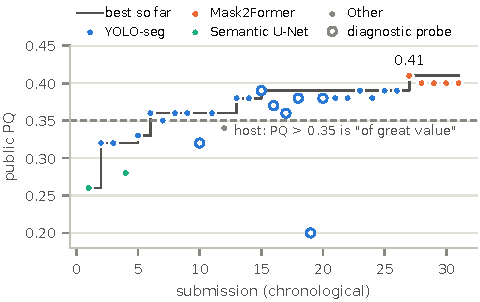
\includegraphics[width=0.8\textwidth]{figures/fig_progress.pdf}
\caption{Public PQ of all \Submissions{} submissions in the order in which they were made,
coloured by model family. Hollow markers are diagnostic probes, which we submitted to learn
something about the leaderboard; we did not expect them to raise the score.
\generatedby{paper/make\_figures.py:figure\_progress}}
\label{fig:intro-progress}
\end{figure}

\begin{table}[t]
\centering\small
\caption{The changes that moved the public score. Validation PQ is measured on our fixed
validation split (Chapter~\ref{ch:validation}).}
\label{tab:intro-milestones}
\begin{tabularx}{\textwidth}{@{}lXcc@{}}
\toprule
experiment & change & validation & public \\
\midrule
exp001 & U-Net++ semantic segmentation, then connected components & 0.2957 & 0.26 \\
exp002 & YOLO11m-seg instance segmentation trained at 1280 px & 0.3736 & 0.32 \\
exp002 & same weights, inference at the native 2048 px & 0.4064 & 0.33 \\
exp005 & erode every predicted mask by one pixel & 0.4404 & 0.36 \\
exp037 & eight-view test-time augmentation with fusion & 0.4571 & 0.38 \\
exp062 & lower emission confidence (0.35) with fusion & 0.4559 & 0.39 \\
exp119 & two-architecture YOLO ensemble & 0.4681 & 0.39 \\
\textbf{exp139} & \textbf{Mask2Former at native resolution, one view} & \textbf{0.4705} & \textbf{0.41} \\
\bottomrule
\end{tabularx}
\end{table}

Figure~\ref{fig:intro-map} groups the approaches we tried into four families and shows where
each is described. It can be read as a table of contents organised by idea.

\begin{figure}[t]
\centering
\begin{tikzpicture}[
  fam/.style={box=#1, text width=2.35cm, minimum height=0.9cm,
              execute at begin node={\hyphenpenalty=10000}},
  leaf/.style={font=\sffamily\scriptsize, text=inksecondary, align=left, text width=2.4cm,
               anchor=north},
  node distance=0.18cm]
  \node[fam=vizaqua] (dense) at (0,0) {\textbf{\color{inkprimary}Dense\\ segmentation}\\ Ch.~\ref{ch:paradigms}};
  \node[fam=vizblue] (yolo) at (2.9,0) {\textbf{\color{inkprimary}YOLO\\ instances}\\ Ch.~\ref{ch:yolo}--\ref{ch:tta}};
  \node[fam=vizyellow] (post) at (5.8,0) {\textbf{\color{inkprimary}Fixing\\ masks}\\ Ch.~\ref{ch:post}};
  \node[fam=inkmuted] (recall) at (8.7,0) {\textbf{\color{inkprimary}Finding\\ misses}\\ Ch.~\ref{ch:recall}};
  \node[leaf] at (0,-0.85) {U-Net++ @512: 0.26\\ U-Net @1024: 0.28\\ spine seeding: $\pm$0\\ centre/offset: $\le$0};
  \node[leaf] at (2.9,-0.85) {train 1280: 0.32\\ infer 2048: 0.33\\ 1 px erosion: 0.36\\ D4 fusion: 0.38--0.39\\ YOLOv8l @2048: 0.39\\ 2-model ensemble: 0.39};
  \node[leaf] at (5.8,-0.85) {refiners: $-$0.008, $-$0.031\\ logit cut, SAM2: $\le$0\\ edge snapping: harmful\\ split, grow: 13--34\%\\ of oracle ceilings};
  \node[leaf] at (8.7,-0.85) {verifiers: $\le$+0.002\\ crop CNN: chance\\ physics proposals keep\\ 26\% of the disk\\ semantic pruning: 0.39};
  \node[fam=vizorange, text width=10.9cm] (m2f) at (4.35,-4.25)
       {\textbf{\color{inkprimary}Mask2Former at native resolution} (Ch.~\ref{ch:transformers}--\ref{ch:submission}):
        first attempt at 1024 px 0.30 validation; proper training 0.4705 validation, \textbf{0.41 public}};
\end{tikzpicture}
\caption{The approaches we tried, grouped by family, with the chapter that describes each. Numbers
are public PQ unless they are marked as a change in validation PQ.
\drawnin{book/chapters/ch01\_introduction.tex}}
\label{fig:intro-map}
\end{figure}

\section{The final model}\label{sec:intro-winner}
Our final model is a single \keyterm{Mask2Former} network~\citep{mask2former} with a Swin-S
backbone~\citep{swin}, trained for 50 epochs on one H100 GPU, and its submission scores
\BestPublic{} on the public leaderboard. Three
design decisions account for most of its performance, and later chapters support each of them
with measurements.
\begin{enumerate}[leftmargin=*,itemsep=2pt]
\item \textbf{Native resolution.} We never shrink the photograph. Mask2Former predicts masks at a
quarter of the resolution of its input, so when the input is the native $2048\times2048$ image
the masks lie on a grid of cells four pixels wide. Section~\ref{sec:train-resolution} shows that a
grid this fine can represent the annotated masks almost perfectly, whereas the coarser grid that
results from a shrunken input cannot.
\item \textbf{Set prediction.} Mask2Former proposes a fixed set of 100 candidate objects, and it is
trained, through a one-to-one matching between candidates and annotated filaments, to propose each
filament only once. As a result it rarely splits a filament into several masks or merges several
filaments into one (Section~\ref{sec:tr-detr}).
\item \textbf{A validation procedure that agrees with the leaderboard.} Our evaluation code
reproduces the organisers' scoring code to nine decimal places, so a decision taken on our
validation split is a decision about the quantity that the leaderboard measures
(Section~\ref{sec:sub-eval}).
\end{enumerate}
On our validation split the model scores a PQ of \HostPQ{}, with a 95\% bootstrap interval of
\PQLow{}--\PQHigh{} over resamples of the validation photographs. Chapter~\ref{ch:submission}
examines what it does well and what it still misses.

\section{How to read this book}\label{sec:intro-read}
Readers who only want to understand the final model can read Chapters~\ref{ch:metric},
\ref{ch:transformers}, \ref{ch:training} and~\ref{ch:submission} after this one. Readers who want
to understand how we arrived at that model should read the chapters in order, since each of
Chapters~\ref{ch:paradigms} to~\ref{ch:recall} ends with the measurements that closed one line of
work and motivated the next. Readers who want to use the masks for solar physics should read
Chapters~\ref{ch:data}, \ref{ch:metric} and~\ref{ch:submission}, which describe the data, what the
score measures, and which filaments the final model finds and which it misses.
Chapter~\ref{ch:lessons}, on experimental method, is best read last.

\section*{Exercises}
\begin{exercise}{Reading the headline numbers}
The deployed model has \NumTP{} true positives, \NumFP{} false positives and \NumFN{} false
negatives on the validation split, and its SQ is \ValSQ{}. Use Equation~\eqref{eq:intro-pq} to
compute its RQ and PQ, and compare your answers with Table~\ref{tab:intro-milestones}.
\end{exercise}

\begin{exercise}{Records and photographs}
Load \file{data/MAGFiLO\_1.0\_Annotations\_kaggle2026\_train.json} with Python's \texttt{json}
module. Count the entries in its \texttt{images} list and the number of distinct values of their
\texttt{file\_name} field. Explain why the two counts differ, and find a photograph that was
labelled three times.
\end{exercise}

\begin{exercise}{Regenerating a figure}
Run \file{book/make\_book\_figures.py} with the arguments given in its docstring. Then modify
\texttt{fig\_annotators} so that it selects the three-annotator photograph with the \emph{fewest}
filaments, and describe how the annotators' disagreement changes.
\end{exercise}

\begin{exercise}{Finding the evidence}
Choose one row of Table~\ref{tab:intro-milestones}. Find the corresponding experiment in
\file{docs/leaderboard-analysis.md} or \file{docs/ACTIVE\_EXPERIMENT.md}, and write down the TP,
FP and FN counts behind its validation score.
\end{exercise}

\chapter{The Sun, the Photographs and the Labels}\label{ch:data}

\section{Introduction}\label{sec:data-intro}
\epigraph{It is a capital mistake to theorize before one has data.}{Sherlock Holmes, in Arthur
Conan Doyle, \emph{A Scandal in Bohemia} \citeyearpar{doyle1891}}

Before we build any model, we need to understand what the photographs show and how their labels
were made. In this chapter we review just enough solar physics to interpret the images
(Section~\ref{sec:data-sun}), describe the telescopes that took them
(Section~\ref{sec:data-gong}) and the annotations that label them
(Section~\ref{sec:data-magfilo}), summarise the rules of the competition
(Section~\ref{sec:data-rules}), and finally draw some conclusions for modelling
(Section~\ref{sec:data-implications}). Several of the facts collected here, such as the width of
a typical filament and the number of annotators per photograph, will determine important design
choices in later chapters.

\section{Enough solar physics to read the pictures}\label{sec:data-sun}
One does not need to be a solar physicist to work on this problem, but a few facts explain what
the photographs show and why the labels look the way they do.

The visible surface of the Sun, the \keyterm{photosphere}, is covered by a thin and hotter layer
called the \keyterm{chromosphere}~\citep{stix2002}. Hydrogen in the chromosphere absorbs and emits light at a
wavelength of 656.3~nm, the red \keyterm{\Ha{} line}. A filter that passes only a narrow band
around this wavelength blocks most of the light from the photosphere, so an \Ha{} image shows the
chromosphere instead. In this light the disk is covered by a mottled pattern of darker and
brighter cells called the \keyterm{chromospheric network}, with bright patches called
\keyterm{plage} around the active regions where sunspots form.

A \keyterm{filament} is a cloud of plasma that is cooler and denser than its surroundings, held
above the surface by the Sun's magnetic field~\citep{mackay2010}. It lies along a
\keyterm{polarity inversion line}, a curve on the surface across which the vertical component of
the magnetic field changes sign. Seen against the bright disk, the cool plasma absorbs \Ha{}
light, so the filament appears as a dark thread. Seen at the edge of the disk against the dark
sky, the same structure glows, and it is then called a \keyterm{prominence}~\citep{parenti2014}. A
filament has a central \keyterm{spine} and often thin side branches called \keyterm{barbs}.
Whether the barbs bear to the left or to the right encodes the filament's \keyterm{chirality}, a
property of its magnetic field~\citep{martin1998}. Filaments persist for days to weeks, drift
across the disk as the Sun rotates (about once every 27 days), and sometimes erupt, which is why
space-weather forecasting is interested in them~\citep{webb2012,magfilo}.

Three consequences of this physics matter for modelling. First, filaments are dark, but darkness
does not identify them, because the chromospheric network covers the same range of intensities.
This is why simple thresholding of the image does not work, as we show in
Section~\ref{sec:recall-physics}. Second, filaments fade gradually into their surroundings. There
is no sharp edge, so the position of a filament's boundary is a judgement made by the annotator;
Figure~\ref{fig:post-profile} in Chapter~\ref{ch:post} plots the intensity across a real
filament. Third, filaments persist. Photographs taken a day apart show the same filaments, and
this affects how we must split the data into training and validation sets
(Section~\ref{sec:val-time}).

Finally, the disk is darker towards its edge. This \keyterm{limb darkening}~\citep{stix2002} occurs because near
the limb our line of sight passes through the solar atmosphere at a grazing angle. It dims both
the filaments and their surroundings there, so a filament near the limb looks different from one
near the centre of the disk.

\section{The GONG network and its photographs}\label{sec:data-gong}
The photographs come from the \keyterm{Global Oscillation Network Group} (GONG), a set of six
identical telescopes placed around the world so that at least one of them can observe the Sun at
any time~\citep{gong,jain2026gong}.\footnote{GONG is operated by the US National Solar Observatory.
It was built to study oscillations of the Sun's surface, and \Ha{} imaging was added to its
stations later to support the monitoring of space weather~\citep{hill2018}.} The stations are at
Big Bear in California (station code Bh), Mauna Loa in
Hawaii (Mh), Learmonth in Australia (Lh), Udaipur in India (Uh), El Teide in the Canary Islands
(Th) and Cerro Tololo in Chile (Ch). Each station records full-disk \Ha{} images. For the
competition, the images were converted from the astronomical FITS format~\citep{pence2010} into 8-bit grey JPEG
files of $2048\times2048$ pixels. The file name records the time of capture and the station; for
example, \file{20140609195854Bh.jpeg} was taken at Big Bear on 9 June 2014 at 19:58:54.

\begin{figure}[t]
\centering
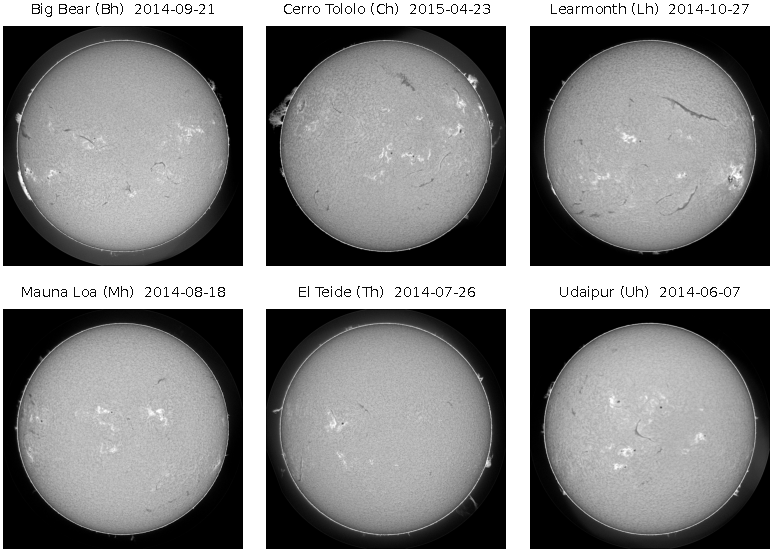
\includegraphics[width=\textwidth]{figures/fig_stations.pdf}
\caption{One training photograph from each GONG station, with the display contrast stretched. The
stations differ in atmospheric seeing, in contrast and in the brightness of the limb. Bright
prominences are visible outside the limb in several of the frames.
\generatedby{book/make\_book\_figures.py:fig\_stations}}
\label{fig:data-stations}
\end{figure}

Figure~\ref{fig:data-stations} shows one photograph from each station. Although the instruments
are identical, the atmosphere above them is not, so the sharpness and contrast of the images vary
from frame to frame, and a model must cope with this variation. On the other hand, the Sun fills
the same circle in every frame, surrounded by black sky, so a model can easily learn where the
disk is.

The training photographs span the years 2011 to 2022, and the test photographs are drawn from the
same years and stations in almost the same proportions (Figure~\ref{fig:data-years}). The dip in
2018--2020 corresponds to the solar minimum, when there are fewer active regions and therefore
fewer filaments to label. We checked this agreement early in the project. A difference between
the training and test distributions, often called \keyterm{covariate shift}, is one of the usual
explanations when validation scores fail to carry over to a leaderboard
(Section~\ref{sec:val-transfer}), and the figure shows that it cannot explain our results.

\begin{figure}[t]
\centering
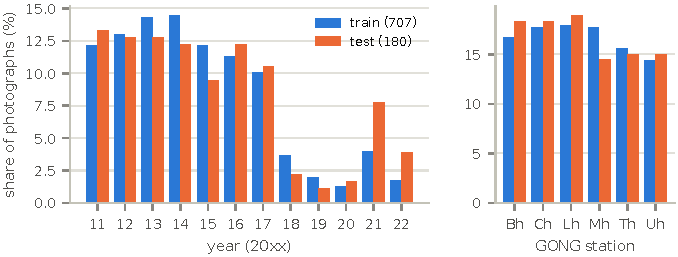
\includegraphics[width=\textwidth]{figures/fig_years.pdf}
\caption{Share of photographs by year (left) and by GONG station (right), for the \AllPhotos{}
training photographs and the \TestPhotos{} test photographs.
\generatedby{book/make\_book\_figures.py:fig\_years}}
\label{fig:data-years}
\end{figure}

\section{The MAGFiLO annotations}\label{sec:data-magfilo}
The labels come from MAGFiLO, the Manually Annotated GONG Filaments in \Ha{} Observations
dataset~\citep{magfilo}, which is released under the Creative Commons BY-NC-ND 4.0 licence. The
competition supplies a subset of it as a single JSON file in the format of the COCO
dataset~\citep{coco}. The file contains three lists that matter to us.
\begin{description}[style=unboxed,leftmargin=1em,itemsep=2pt,font=\normalfont\bfseries]
\item[\texttt{images}] One entry per \emph{annotation record}. Its \texttt{id} joins an
annotator's batch number to the name of the photograph, as in \texttt{040301-20140609195854Bh},
and its \texttt{file\_name} names the photograph.
\item[\texttt{annotations}] One entry per filament, containing a \texttt{segmentation} polygon,
a \texttt{spine} polyline along the filament's centre, a \texttt{bbox}, an \texttt{area}, a
\texttt{category\_id}, and the \texttt{image\_id} of the record the filament belongs to.
\item[\texttt{categories}] Four labels, \emph{Left}, \emph{Right}, \emph{Unidentifiable} and
\emph{Ambiguous}, which record the filament's chirality. The competition ignores them and treats
every filament simply as a filament.
\end{description}

Listing~\ref{lst:data-load} reads the file and groups the records by photograph. Every data
loader in the repository has essentially this shape.

\begin{lstlisting}[caption={Grouping annotation records by photograph. Adapted from \file{shared/data\_split.py:load\_records}.},label=lst:data-load]
import json
from collections import defaultdict

coco = json.load(open("data/MAGFiLO_1.0_Annotations_kaggle2026_train.json"))
records_by_photo = defaultdict(list)      # file_name -> [record id, ...]
for image in coco["images"]:
    records_by_photo[image["file_name"]].append(image["id"])
filaments = defaultdict(list)             # record id -> [annotation, ...]
for annotation in coco["annotations"]:
    filaments[annotation["image_id"]].append(annotation)

print(len(coco["images"]), "records of", len(records_by_photo), "photographs")
print(len(coco["annotations"]), "filaments")
\end{lstlisting}

The listing prints \AllRecords{} records of \AllPhotos{} photographs and \AllFilaments{}
filaments. Of the photographs, \OnceAnnotated{} were labelled once, \TwiceAnnotated{} twice and
\ThriceAnnotated{} three times, by independent annotators who did not see each other's work.
Figure~\ref{fig:intro-annotators} in Chapter~\ref{ch:intro} showed how different their results
can be.

\subsection{Records and photographs}\label{sec:data-records}
Since some photographs have several records, we must decide whether the unit of our data is the
photograph or the record. The metric answers this question for us. As we will see in
Section~\ref{sec:metric-pooling}, each record is scored separately, against the one annotator who
made it. A model that is scored against three annotators on the same photograph is therefore
asked three slightly different questions, one per annotator. For this reason the final model
treats every record as a separate training sample (Section~\ref{sec:train-sampling}): a
photograph with three records is seen three times, each time with one annotator's masks.

Getting this unit wrong has real consequences. In Chapter~\ref{ch:recall} we describe a
classifier that we trained to decide whether a candidate mask was a real filament. We labelled a
candidate as positive if \emph{any} annotator of the photograph had drawn a filament at that
location. The classifier learned this task well, with a precision of 72\% on its own validation
data, but when we used it to choose which candidates to submit, only 17\% of its choices matched
the annotator of the record being scored (Section~\ref{sec:recall-verifiers}). The classifier had
answered the question ``would somebody draw this?'', whereas the metric asks ``did this particular
person draw it?''.

\subsection{How big are filaments?}\label{sec:data-sizes}
Figure~\ref{fig:data-stats} summarises the sizes of the annotated filaments. The median bounding
box is \LongPfifty{} pixels on its long side; 90\% of filaments are shorter than \LongPninety{}
pixels and 99\% are shorter than \LongPninetynine{}, and the longest is \LongMax{} pixels long.
The median area is \AreaMedian{} pixels. A record contains \MeanPerRecord{} filaments on average
and at most \MaxPerRecord{}, and no record is empty.

\begin{figure}[t]
\centering
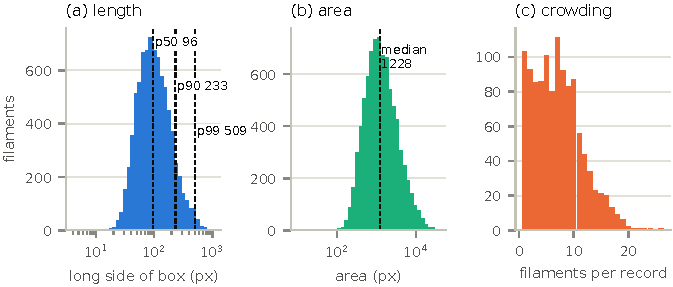
\includegraphics[width=\textwidth]{figures/fig_filament_stats.pdf}
\caption{Filament sizes and crowding over all \AllFilaments{} training annotations. (a) The long
side of the bounding box, with the 50th, 90th and 99th percentiles marked. (b) The area. (c) The
number of filaments per annotation record.
\generatedby{book/make\_book\_figures.py:fig\_filament\_stats}}
\label{fig:data-stats}
\end{figure}

These numbers will turn into design decisions later. Since 99\% of filaments are shorter than
about 510 pixels, a $1024\times1024$ crop centred on a filament almost always contains it whole,
which is why the final model trains on crops of that size (Section~\ref{sec:train-sampling}).
Since a record contains at most \MaxPerRecord{} filaments, a model that proposes 100 candidate
objects per image always has enough of them (Section~\ref{sec:tr-m2f}). And since filament bodies
are only a few pixels wide, resolution matters a great deal: a body four pixels wide in the
native $2048\times2048$ image is only one pixel wide after the image is shrunk to
$512\times512$.

\subsection{Spines}\label{sec:data-spines}
Every annotation also contains a spine, a polyline traced along the filament's axis. We used the
spines in two experiments. The first (exp004) planned to use predicted spines to decide which
pixels belong to which filament, and an ablation led us to drop the idea before any model was
trained (Section~\ref{sec:paradigms-fragments}). The second (exp085) trained a semantic model with
an additional output that predicts the spine (Section~\ref{sec:recall-semantic}). Neither became
part of the final pipeline. Nevertheless, the spine is the most direct description of a
filament's shape, and it remains a natural input for future work.

\section{The competition's rules}\label{sec:data-rules}
The rules of the competition shape the work as much as the data do.
\begin{itemize}[leftmargin=*,itemsep=2pt]
\item \textbf{Submission format.} A submission contains one CSV row per predicted filament: an
identifier of the form \texttt{<photograph>\_<k>}, and the mask as a COCO run-length encoding
without its size field, since the size is always $2048\times2048$ (Chapter~\ref{ch:masks}).
\item \textbf{No overlaps.} The masks predicted for one photograph must be disjoint. The scorer
rejects a file in which two masks share a pixel.
\item \textbf{The leaderboard.} The public leaderboard scores about half of the test photographs
and displays the score to two decimal places. The final ranking uses the other half.
\item \textbf{The rubric.} The final judgement is 70\% quantitative and 30\% qualitative. The
quantitative part uses PQ together with the distributions of the Dice coefficient, of IoU and of
the one-to-many relations between predicted and annotated filaments. The qualitative part is based
on a four-page technical report and on the code. The competition's host has also said that the
judges will look at individual predictions and at the logic of the algorithm, and not only at
the score.
\end{itemize}

\subsection{A replaced evaluator and a data leak}\label{sec:data-history}
Two episodes in the competition's history explain some odd features of its leaderboard. Before
August 2026 the competition was scored with a metric based on the Dice coefficient, and this
metric could be exploited: a public notebook showed that submitting empty masks for five of the
180 test images produced a perfect score of 1.00. The organisers replaced the metric with
Panoptic Quality and rescored all submissions. Some very high scores that remain on the
leaderboard still come from methods that, according to the host, can be distinguished from
legitimate work.

The second episode is a leak. The full MAGFiLO dataset is public, and it contains the
competition's test photographs together with their annotations. Training on it would mean
training on the answers, so we never use it. The release is also smaller than it first appears.
The MAGFiLO paper reports 1,593 observations, but this number counts annotation passes; the
release contains 958 distinct photographs, of which the competition already uses 887.

\section{What the data imply for modelling}\label{sec:data-implications}
We end the chapter by collecting the facts above into five implications, each of which we will
meet again.
\begin{enumerate}[leftmargin=*,itemsep=2pt]
\item Resolution matters. Filaments are a few pixels wide, and shrinking the image destroys them
(Sections~\ref{sec:yolo-resolution} and~\ref{sec:train-resolution}).
\item Labels belong to records. We should train, and score, one annotator at a time
(Section~\ref{sec:data-records}).
\item Labels disagree. No model can match every annotator perfectly, so a perfect score is not a
useful reference point (Section~\ref{sec:metric-agreement}).
\item Photographs are not independent. The same filament appears in photographs taken days apart,
so a random split of the photographs leaks information from training to validation
(Section~\ref{sec:val-time}).
\item Position matters. Limb darkening and foreshortening make a filament near the edge of the disk
look different from one near its centre.
\end{enumerate}

\section*{Exercises}
\begin{exercise}{Decoding file names}
Write a function that turns \file{20110914063134Lh.jpeg} into a timestamp and a station name. Use
it to count the training photographs per station, and compare your counts with
Figure~\ref{fig:data-years}.
\end{exercise}

\begin{exercise}{Long filaments}
Using the \texttt{bbox} field, compute the fraction of filaments whose long side exceeds 512
pixels. Relate your answer to the crop size used in Chapter~\ref{ch:training}.
\end{exercise}

\begin{exercise}{Spine and polygon}
Choose one annotation, draw its polygon and its spine on the same axes, and compute the length of
the spine. Is the spine always inside the polygon?
\end{exercise}

\begin{exercise}{Chirality}
Count how often each of the four \texttt{category\_id} values occurs. Then, for photographs with
more than one annotator, estimate how often two annotators give the same category to a filament
that both of them drew. What does your answer suggest about using the categories as a training
signal?
\end{exercise}

\chapter{Pixels, Polygons and Run-Length Encoding}\label{ch:masks}

\section{Introduction}\label{sec:masks-intro}
A segmentation model produces masks, the annotations are stored as polygons, and the competition's
scorer compares masks that are stored as compressed strings of text. In this chapter we study
these representations and the operations that connect them. Section~\ref{sec:masks-raster}
explains how a polygon is turned into a mask and why the details of that conversion matter so much
for thin objects. Section~\ref{sec:masks-rle} describes the run-length encoding used in the
submission file. Section~\ref{sec:masks-iou} defines the two standard measures of overlap between
masks, and Section~\ref{sec:masks-paint} describes how we turn a set of overlapping candidate masks
into the disjoint set that the rules require. These operations may look like routine plumbing, but
the first of them turned out to explain one of the largest improvements we made
(Section~\ref{sec:yolo-erosion}).

\section{From polygons to pixels}\label{sec:masks-raster}
A \keyterm{mask} is a binary image $M\in\{0,1\}^{H\times W}$, with $M_{ij}=1$ when pixel $(i,j)$
belongs to the object. An annotation, by contrast, is a polygon whose vertices have real-valued
coordinates. Converting a polygon into a mask is called \keyterm{rasterisation}, and it requires a
rule for the pixels that the boundary passes through. Is such a pixel inside the object if its
centre is inside the polygon? If any part of it is? If most of it is? Different software libraries
answer this question differently.

For a large, compact object the choice hardly matters, because the boundary pixels are a small
fraction of the total. A filament, however, is thin, so a large fraction of its pixels lie on or
near its boundary. Measured over the training annotations, the ratio of perimeter to area is about
$P/A=0.216$ per pixel. Suppose that two rasterisation rules place the boundary at positions that
differ by a distance $\delta$ all along its length. The area between the two boundaries is roughly
the perimeter times the offset, so the relative difference in area is
\begin{equation}
\frac{\Delta A}{A}\approx\frac{\delta\,P}{A}=0.216\,\delta .
\label{eq:masks-offset}
\end{equation}
A disagreement of only half a pixel therefore changes a filament's area by about 11\%.

\begin{figure}[t]
\centering
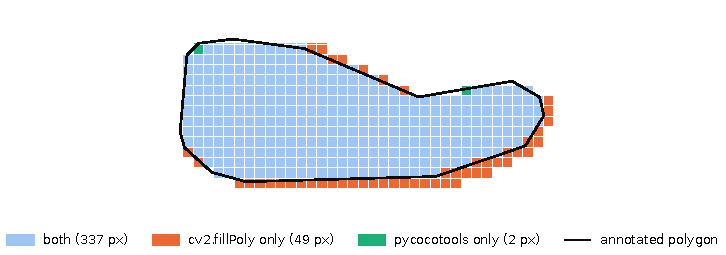
\includegraphics[width=\textwidth]{figures/fig_raster.pdf}
\caption{The same annotated polygon rasterised by two libraries. \texttt{cv2.fillPoly}, which
Ultralytics uses to build YOLO training targets, marks \RasterCv{} pixels; \texttt{pycocotools},
which the organisers' scorer uses, marks \RasterCoco{}. The IoU of the two masks is \RasterIoU{}.
\generatedby{book/make\_book\_figures.py:fig\_raster}}
\label{fig:masks-raster}
\end{figure}

Figure~\ref{fig:masks-raster} shows the effect on one real, thin filament. To measure it more
generally, we rasterised 400 randomly sampled training filaments with three common libraries (the
COCO tools \texttt{pycocotools}~\citep{coco}, OpenCV's \texttt{cv2}~\citep{bradski2000} and PIL)
and compared the results pair by pair (exp006):
\begin{center}\small
\begin{tabular}{@{}lcc@{}}
\toprule
pair of rasterisers & mean IoU & mean area relative to pycocotools \\
\midrule
pycocotools and cv2 & 0.874 & cv2 $+7.96\%$ \\
pycocotools and PIL & 0.915 & PIL $+5.71\%$ \\
cv2 and PIL & 0.897 & -- \\
\bottomrule
\end{tabular}
\end{center}
Two masks of the same polygon, both produced by standard software, agree with an IoU of less than
0.9. We will see in Chapter~\ref{ch:metric} that the metric requires an IoU above 0.5 before a
prediction counts at all, so a systematic error of this size uses up a substantial part of the
margin.

\subsection{Example: why the YOLO masks were too wide}\label{sec:masks-fat}
The competition's scorer rasterises the annotations with \texttt{pycocotools}. Ultralytics, the
library we used to train the YOLO models of Chapter~\ref{ch:yolo}, rasterises its training targets
with \texttt{cv2.fillPoly}. When we measured this end to end on our own pipeline, the YOLO training
targets agreed with the masks that the scorer uses with an IoU of 0.902, and they were
\textbf{10.8\% larger} on average, which is close to the value predicted by
Equation~\eqref{eq:masks-offset}. A model trained on these targets learns to draw every filament
slightly too wide, however well it is trained.

We noticed the effect before we understood it. In experiment exp005 we tried to \emph{grow} the
predicted masks, expecting that the model was cutting off thin barbs. Every amount of growth
lowered the score, whereas eroding every mask by one pixel raised it: validation PQ rose from
0.4169 to 0.4404, and the public score from 0.33 to 0.36, the largest single improvement of the
YOLO period. Section~\ref{sec:yolo-erosion} describes that experiment. The mismatch between the two
rasterisers explains about 95\% of the gain.

\subsection{Correcting in coordinates rather than pixels}\label{sec:masks-shrink}
Eroding a binary mask by one pixel is a coarse correction. It changed the area of the YOLO masks
from about 11\% too large to about 10\% too small. The ideal correction is half a pixel, and a
binary mask cannot be moved by half a pixel. To see why, consider the distance
transform~\citep{borgefors1986} of the mask, which gives each foreground pixel its distance to the
nearest background pixel. Every
boundary pixel is at distance 1, so thresholding the distance transform at 0.25, 0.5 or 0.75
returns the original mask unchanged.

Polygon coordinates have no such limitation. If we shrink each polygon inward by a fraction of a
pixel \emph{before} rasterising it, the correction is exact. We measured the effect of an inward
offset $\delta$ on 250 instances (exp006):
\begin{center}\small
\begin{tabular}{@{}lcccccc@{}}
\toprule
inward offset $\delta$ (px) & 0 & 0.25 & 0.35 & \textbf{0.50} & 0.65 & 1.00 \\
\midrule
IoU with the scorer's mask & 0.898 & 0.946 & 0.955 & \textbf{0.959} & 0.945 & 0.876 \\
area ratio & 1.112 & 1.039 & 1.019 & \textbf{0.986} & 0.954 & 0.876 \\
\bottomrule
\end{tabular}
\end{center}
An offset of half a pixel raises the agreement with the scorer from an IoU of 0.898 to 0.959.
Listing~\ref{lst:masks-shrink} shows the correction. It uses a polygon \emph{buffer}, which moves
every edge inward by the same perpendicular distance. Scaling the polygon towards its centroid
would be simpler, but it would move the ends of a long curved filament much further than its
middle. The code also guards against two failure modes that a naive buffer has on thin shapes. A
buffer can split a polygon at a narrow waist, which happened to 42 of the \AllFilaments{} training
filaments; in that case we keep the largest piece, so that one annotated filament never becomes two
training targets. A buffer can also erase a very thin shape altogether; in that case we keep the
original polygon.

\begin{lstlisting}[caption={Half-pixel inward offset for YOLO training targets. Simplified from \file{experiments/exp\_002\_yolo\_seg/src/prepare\_yolo.py:shrink}.},label=lst:masks-shrink]
from shapely.geometry import Polygon

def shrink(polygon, offset):
    """Offset a polygon inward by `offset` pixels, in coordinate space."""
    if offset <= 0 or len(polygon) < 3:
        return [polygon]
    shape = Polygon(polygon)
    if not shape.is_valid:
        shape = shape.buffer(0)          # repairs self-intersecting traces
    shrunk = shape.buffer(-offset)
    if shrunk.is_empty:                  # a very thin filament: keep the original
        return [polygon]
    geoms = [shrunk] if shrunk.geom_type == "Polygon" else list(shrunk.geoms)
    # One filament in, one filament out: if a narrow waist split it,
    # keep only the largest piece, never two instances where one was drawn.
    largest = max(geoms, key=lambda g: g.area)
    return [np.asarray(largest.exterior.coords, dtype=np.float64)]
\end{lstlisting}

The whole effect described in this section is invisible to a test that rasterises the ``ground
truth'' and the ``prediction'' with the same library, because such a test builds the answer into
its assumptions. We found the mismatch only by comparing the real training targets with the masks
that the real scorer computes. We return to this point in Chapter~\ref{ch:lessons}.

\section{Run-length encoding}\label{sec:masks-rle}
A $2048\times2048$ binary mask contains about four million pixels. Stored as one byte per pixel it
would occupy 4\,MB, but the competition's CSV file stores it in a few hundred bytes using the
\keyterm{run-length encoding} (RLE) of the COCO dataset~\citep{coco}. The idea is simple. We flatten the mask
into one long vector and record only the lengths of the alternating runs of zeros and ones.

COCO fixes two conventions. First, the flattening is \keyterm{column-major}: we read down the
first column, then down the second, and so on.\footnote{Column-major order is the convention of
Fortran and MATLAB, which is why NumPy~\citep{harris2020} calls arrays stored this way
``Fortran-ordered''.} Second, the first run always counts zeros, so a mask
whose first pixel is a one begins with a run of length zero. Figure~\ref{fig:masks-rle} works
through a $6\times6$ example.

\begin{figure}[t]
\centering
\begin{tikzpicture}[scale=0.42]
  \foreach \c/\r in {1/1,1/2,2/1,2/2,2/3,3/2,3/3,3/4,4/3,4/4} {
    \fill[vizblue!55] (\c,-\r) rectangle ++(1,-1);
  }
  \draw[step=1, gridline!80!black, line width=0.3pt] (0,0) grid (6,-6);
  \draw[inkprimary, line width=0.6pt] (0,0) rectangle (6,-6);
  \foreach \c in {0,...,5} \draw[->, vizorange, line width=0.6pt] (\c+0.5,0.25) -- (\c+0.5,-0.2);
  \node[note, anchor=south] at (3,0.4) {read each column top to bottom, left to right};
  \node[anchor=west, font=\ttfamily\scriptsize, text=inkprimary, align=left] at (7,-1.3)
    {0000000 11 0000 111 0000 111 0000 11 0000000};
  \node[anchor=west, note, align=left] at (7,-2.5) {runs: 7, 2, 4, 3, 4, 3, 4, 2, 7 \ \ (zeros first)};
  \node[anchor=west, note, align=left] at (7,-3.7) {differences from the run two back (from the fourth):\\ 7, 2, 4, 1, 0, 0, 0, $-$1, 3};
  \node[anchor=west, font=\ttfamily\small, text=inkprimary] at (7,-5.2) {counts = "7241000O3"};
\end{tikzpicture}
\caption{Run-length encoding of a $6\times6$ mask with 10 foreground pixels. Flattening the mask in
column-major order gives nine runs. COCO then stores each run from the fourth onwards as its
difference from the run two places earlier, writes each number in groups of 5 bits, and adds 48 to
every group so that it prints as an ASCII character. The string shown was produced by
\texttt{pycocotools}. \drawnin{book/chapters/ch03\_masks.tex}}
\label{fig:masks-rle}
\end{figure}

\subsection{The compressed string *}\label{sec:masks-rle-string}
A plain list of run lengths would still waste space on long runs, so COCO compresses it further.
Each run length, from the fourth onwards, is replaced by its \emph{difference} from the run length
two positions earlier. Consecutive columns of a filament tend to have similar runs, so these
differences are small. Each number is then split into groups of 5 bits, lowest bits first; a sixth
bit in each group marks whether another group follows; and 48 is added to the result so that it is
a printable character. In the example of Figure~\ref{fig:masks-rle}, the eighth run is 2 and the
sixth is 3, so the stored difference is $-1$. In two's complement arithmetic the lowest five bits
of $-1$ are 31, no further group is needed, and $31+48=79$ is the character \texttt{O}. The whole
mask becomes the nine characters \texttt{7241000O3}.

\subsection{Encoding and decoding in practice}\label{sec:masks-rle-code}
In practice we never write this encoder ourselves. Listing~\ref{lst:masks-rle} shows the two helper
functions through which every one of our submissions passes. The only subtle detail is the call to
\texttt{np.asfortranarray}. The \texttt{pycocotools} library expects the mask in column-major
memory order, and if it is given an ordinary row-major NumPy array it silently encodes the
transposed mask.

\begin{lstlisting}[caption={Encoding and decoding submission masks. From \file{shared/utils.py}.},label=lst:masks-rle]
from pycocotools import mask as mask_util

def encode_rle(binary_mask):
    """A binary (H, W) mask -> the COCO RLE `counts` string of the submission."""
    mask = np.asfortranarray(binary_mask.astype(np.uint8))
    return mask_util.encode(mask)["counts"].decode("utf-8")

def decode_rle(counts, size=(2048, 2048)):
    rle = {"size": list(size), "counts": counts.encode("utf-8")}
    return mask_util.decode(rle)
\end{lstlisting}

RLE is also the right format for storing masks between processing steps. On one occasion we cached
dense $2048\times2048$ masks for a parameter sweep; this took about 9\,GB per level of erosion, and
the process was killed for lack of memory. The same masks stored as RLE take a few kilobytes each.
The functions \texttt{pycocotools.mask.iou} and \texttt{pycocotools.mask.area} also operate
directly on RLE, so most measurements never need a dense mask at all.

\section{Comparing masks: IoU and Dice}\label{sec:masks-iou}
There are two standard ways to compare a predicted mask $A$ with an annotated mask $B$. The
\keyterm{intersection over union}, which ecologists know as the Jaccard index~\citep{jaccard1912},
is
\begin{equation}
\IoU(A,B)=\frac{|A\cap B|}{|A\cup B|},
\end{equation}
and the \keyterm{Dice coefficient}~\citep{dice1945} is
\begin{equation}
\mathrm{Dice}(A,B)=\frac{2|A\cap B|}{|A|+|B|}.
\end{equation}
Both are 1 for identical masks and 0 for disjoint ones, and in fact each can be computed from the
other. Writing $I=|A\cap B|$ and $U=|A\cup B|=|A|+|B|-I$, we have $\mathrm{Dice}=2I/(U+I)$, and
dividing the numerator and denominator by $U$ gives
\begin{equation}
\mathrm{Dice}=\frac{2\,\IoU}{1+\IoU},\qquad \IoU=\frac{\mathrm{Dice}}{2-\mathrm{Dice}}.
\label{eq:masks-dice-iou}
\end{equation}
Since $\IoU\le1$, Dice is never smaller than IoU. This is why the mean Dice of our final model
over overlapping pairs (\MeanDiceOverlap{}) looks better than its mean IoU (\MeanIoUOverlap{}),
although the two numbers describe the same masks. The leaderboard uses IoU, through Panoptic
Quality; the competition's rubric also asks for the distribution of Dice.

For thin objects both measures are very sensitive to small displacements. Consider a long filament
four pixels wide, and a copy of it shifted sideways by one pixel. Ignoring the ends, the
intersection is three pixels wide and the union five, so the IoU is $3/5=0.6$. With a shift of two
pixels the IoU falls to $2/6\approx0.33$, which is below the value of 0.5 that the metric requires
for a match. A disagreement of a few pixels about where a filament's edge lies can therefore decide
whether a prediction counts as a success or as two errors.

\section{From candidates to disjoint instances: painting}\label{sec:masks-paint}
Models do not naturally produce disjoint masks. A detector proposes candidates that may overlap,
while the scorer rejects any submission whose masks overlap. We resolve overlaps with a simple
procedure that we call \keyterm{painting}, close to the heuristic that \citet{pq} use to turn
instance predictions into a panoptic output, summarised in Algorithm~\ref{alg:masks-paint} and
Figure~\ref{fig:masks-paint}. We sort the candidates by their confidence scores, highest first.
Each candidate in turn keeps only those of its pixels that no higher-scoring candidate has already
claimed, and it is discarded if too few pixels remain.

\begin{algorithmblock}{Painting: turning scored candidates into disjoint masks\label{alg:masks-paint}}
\item \textbf{input:} candidates $(s_k, m_k)$, each a score and a binary mask; minimum area $a_{\min}$
\item sort the candidates so that $s_1\ge s_2\ge\cdots$;
\item $C\leftarrow$ empty mask (the pixels claimed so far); $\mathcal{S}\leftarrow\emptyset$;
\item \textbf{for} $k=1,2,\dots$ \textbf{do}
\item \Ind $r_k\leftarrow m_k\wedge\neg C$ \quad (the pixels of $m_k$ not yet claimed);
\item \Ind \textbf{if} $|r_k|\ge a_{\min}$ \textbf{then} add $(s_k, r_k)$ to $\mathcal{S}$ and set $C\leftarrow C\vee r_k$;
\item \textbf{return} $\mathcal{S}$
\end{algorithmblock}

\begin{figure}[t]
\centering
\begin{tikzpicture}[scale=0.62]
  \begin{scope}
    \fill[vizblue!45] (0,0) ellipse (1.6 and 0.55);
    \fill[vizorange!45, rotate around={35:(1.0,0.2)}] (1.0,0.2) ellipse (1.5 and 0.45);
    \draw[vizblue!80!black, line width=0.7pt] (0,0) ellipse (1.6 and 0.55);
    \draw[vizorange!80!black, line width=0.7pt, rotate around={35:(1.0,0.2)}] (1.0,0.2) ellipse (1.5 and 0.45);
    \node[note] at (0,-1.3) {two candidates overlap};
    \node[note, text=vizblue!80!black] at (-1.2,0.95) {score 0.93};
    \node[note, text=vizorange!80!black] at (2.4,1.35) {score 0.88};
  \end{scope}
  \draw[flow] (3.4,0) -- (4.6,0);
  \begin{scope}[xshift=7cm]
    \begin{scope}
      \clip (-3,-2) rectangle (3,2);
      \fill[vizorange!45, rotate around={35:(1.0,0.2)}] (1.0,0.2) ellipse (1.5 and 0.45);
      \fill[vizblue!45] (0,0) ellipse (1.6 and 0.55);
    \end{scope}
    \draw[vizblue!80!black, line width=0.7pt] (0,0) ellipse (1.6 and 0.55);
    \node[note] at (0,-1.3) {the higher score keeps the overlap;\\ the other keeps only unclaimed pixels};
  \end{scope}
\end{tikzpicture}
\caption{Painting resolves overlaps. Candidates are placed in order of decreasing score, and each
keeps only the pixels that no earlier candidate has claimed. \drawnin{book/chapters/ch03\_masks.tex}}
\label{fig:masks-paint}
\end{figure}

\begin{lstlisting}[caption={Overlap resolution by painting. From \file{shared/utils.py:paint\_panoptic}.},label=lst:masks-paint]
def paint_panoptic(candidates, min_area=150, image_size=(2048, 2048)):
    """Resolve overlapping (score, mask) candidates into a pixel-disjoint set."""
    ordered = sorted(candidates, key=lambda c: -c[0])
    claimed = np.zeros(image_size, dtype=np.uint8)
    kept = []
    for score, binary in ordered:
        remaining = (binary.astype(np.uint8) & (1 - claimed)).astype(np.uint8)
        area = int(remaining.sum())
        if area < min_area:
            continue
        claimed |= remaining
        kept.append((score, remaining, area))
    return kept
\end{lstlisting}

Painting has two properties that we will use later. First, a candidate can never take pixels from
a candidate with a higher score. Adding low-scoring candidates to the pool therefore cannot destroy
a match that already exists, which is why the recall experiments of Chapter~\ref{ch:recall} could
only ever cost us false positives and never lost true positives. Second, the minimum area is
applied \emph{after} the overlaps have been removed, so a candidate that loses most of its pixels
to a neighbour disappears altogether. The final model uses a minimum area of 100 pixels, and the
YOLO models used 300.

\section*{Exercises}
\begin{exercise}{The boundary approximation}
Derive Equation~\eqref{eq:masks-offset} for a rectangle of length $L$ and width $w$ that is shrunk
inward by $\delta$ on every side, and find the conditions under which the approximation is poor.
For a filament with $w=4$ pixels, what inward offset changes the area by 25\%?
\end{exercise}

\begin{exercise}{Encoding by hand}
Encode the transpose of the mask in Figure~\ref{fig:masks-rle} by hand, and check your string with
\texttt{pycocotools.mask.encode}. Then repeat the encoding without \texttt{np.asfortranarray}, and
explain the result.
\end{exercise}

\begin{exercise}{Dice and IoU}
Prove Equation~\eqref{eq:masks-dice-iou}, and show that $\mathrm{Dice}\ge\IoU$, with equality only
at 0 and 1. What value of Dice corresponds to the matching threshold $\IoU=0.5$?
\end{exercise}

\begin{exercise}{Painting order}
Write a test for \texttt{paint\_panoptic} that uses three overlapping random masks. Check that the
output is pixel-disjoint and that permuting the input does not change it. What happens when two
candidates have exactly the same score?
\end{exercise}

\begin{exercise}{A rasteriser audit}
Reproduce the first table of Section~\ref{sec:masks-raster} for 400 random training filaments, and
plot the ratio of the \texttt{cv2} area to the \texttt{pycocotools} area against each filament's
ratio of perimeter to area. Does the slope agree with Equation~\eqref{eq:masks-offset}?
\end{exercise}

\chapter{Panoptic Quality}\label{ch:metric}

\section{Introduction}\label{sec:metric-intro}
\epigraph{When you can measure what you are speaking about, and express it in numbers, you know
something about it.}{Lord Kelvin, in a lecture of 3 May 1883, printed in \citet{kelvin1889}}

The competition scores every submission with a single number, the \keyterm{Panoptic Quality}
(PQ). The metric was introduced by \citet{pq} for panoptic segmentation, and the competition uses
its instance-segmentation form.\footnote{\citet{pq} proposed panoptic segmentation as a single
task that unifies semantic segmentation (``stuff'') and instance segmentation (``things''), and
designed PQ to score both kinds of region with one formula.} Since every result in this book is a PQ number, it pays to
understand the metric thoroughly: what it rewards, what it punishes, and how much each kind of
mistake costs. In Section~\ref{sec:metric-matching} we define how predictions are matched to
annotations, and in Section~\ref{sec:metric-sqrq} we split PQ into two factors that measure
delineation and detection separately. Section~\ref{sec:metric-pooling} explains how the counts
from different annotators are combined. Section~\ref{sec:metric-leverage} works out how much each
kind of change to a submission is worth, a calculation we will use throughout the book.
Sections~\ref{sec:metric-agreement} and~\ref{sec:metric-uncertainty} ask how well human annotators
agree with each other, and how precisely a PQ value measured on a finite validation set can be
trusted. Finally, Section~\ref{sec:metric-code} compares the organisers' implementation of the
metric with ours.

\section{Matching predictions to annotations}\label{sec:metric-matching}
Consider one photograph, one annotator's record of it, and the set of masks that a model predicted
for that photograph. The first step of the metric pairs predictions with annotations. A predicted
mask $p$ and an annotated mask $g$ \keyterm{match} when
\begin{equation}
\IoU(p,g)=\frac{|p\cap g|}{|p\cup g|}>\tfrac12 .
\end{equation}
Matched pairs are called \keyterm{true positives}. A prediction that matches no annotation is a
\keyterm{false positive}, and an annotation that matches no prediction is a \keyterm{false
negative}.

It is not obvious that this rule defines a proper matching. Could one annotation match two
predictions, so that it would be counted twice? The following result shows that it cannot,
provided that the predictions do not overlap each other, which the competition requires.

\begin{theorem}[matches above an IoU of one half are unique]\label{thm:metric-unique}
If the predicted masks are pairwise disjoint, then each annotation matches at most one prediction.
Likewise, since the annotated masks of one record are pairwise disjoint, each prediction matches at
most one annotation.
\end{theorem}
\begin{proof}
If $\IoU(p,g)>\tfrac12$, then $|p\cap g|>\tfrac12|p\cup g|\ge\tfrac12|g|$, so a prediction that
matches $g$ covers more than half of $g$. If two disjoint predictions $p_1$ and $p_2$ both matched
$g$, then $p_1\cap g$ and $p_2\cap g$ would be disjoint subsets of $g$, each containing more than
half of its pixels, which is impossible. The second statement follows by exchanging the roles of
predictions and annotations.
\end{proof}

Theorem~\ref{thm:metric-unique} has a useful practical consequence. The organisers' notebook marks
\emph{every} pair above the threshold as a true positive, whereas our own evaluator performs a
greedy one-to-one matching in order of decreasing IoU. For disjoint masks the two procedures produce
the same pairs, so there is no need for an optimal assignment algorithm such as the Hungarian
method~\citep{kuhn,munkres1957}, and the two
implementations agree (Section~\ref{sec:metric-code}).

\section{Segmentation quality and recognition quality}\label{sec:metric-sqrq}
Given the matches, Panoptic Quality is defined as
\begin{equation}
\PQ=\frac{\sum_{(p,g)\in\TP}\IoU(p,g)}{|\TP|+\tfrac12|\FP|+\tfrac12|\FN|}.
\label{eq:metric-pq}
\end{equation}
The numerator rewards each true positive by the quality of its mask. The denominator counts every
true positive once and charges half a unit for every false positive and every false negative.
Multiplying and dividing by $|\TP|$ splits PQ into two factors with separate meanings:
\begin{equation}
\PQ=\underbrace{\frac{1}{|\TP|}\sum_{(p,g)\in\TP}\IoU(p,g)}_{\textstyle\SQ}
\;\times\;
\underbrace{\frac{|\TP|}{|\TP|+\tfrac12|\FP|+\tfrac12|\FN|}}_{\textstyle\RQ}.
\label{eq:metric-sqrq}
\end{equation}
The \keyterm{segmentation quality} (SQ) is the mean IoU of the matched pairs, so it measures how
well the filaments that were found have been outlined. The \keyterm{recognition quality} (RQ)
measures detection. In fact RQ is the familiar $F_1$ score~\citep{vanrijsbergen1979} of detection at an IoU threshold of one
half. With precision $|\TP|/(|\TP|+|\FP|)$ and recall $|\TP|/(|\TP|+|\FN|)$, we have
\begin{equation}
F_1=\frac{2\,\mathrm{precision}\cdot\mathrm{recall}}{\mathrm{precision}+\mathrm{recall}}
    =\frac{2|\TP|}{2|\TP|+|\FP|+|\FN|}=\RQ .
\end{equation}

\subsection{Example: scoring one record by hand}\label{sec:metric-example}
Suppose that an annotator drew four filaments $g_1,\dots,g_4$ on a photograph, and that the model
predicted four disjoint masks $p_1,\dots,p_4$. Suppose further that $\IoU(p_1,g_1)=0.80$,
$\IoU(p_2,g_2)=0.60$ and $\IoU(p_3,g_3)=0.45$, that $p_4$ overlaps no annotation, and that nothing
was predicted near $g_4$. The first two pairs match. The third does not, because its IoU is below
one half, so $p_3$ counts as a false positive and $g_3$ as a false negative. In total we have two
true positives, two false positives ($p_3$ and $p_4$) and two false negatives ($g_3$ and $g_4$).
Hence
\begin{gather*}
\SQ=\frac{0.80+0.60}{2}=0.70,\qquad
\RQ=\frac{2}{2+\tfrac12\cdot2+\tfrac12\cdot2}=0.50,\\
\PQ=\SQ\times\RQ=0.35 .
\end{gather*}
Now suppose that a better model draws $p_3$ slightly more accurately, so that its IoU with $g_3$
rises from 0.45 to 0.55. The pair now matches, and we have three true positives, one false
positive and one false negative. The numerator becomes $0.80+0.60+0.55=1.95$, the denominator
becomes $3+\tfrac12+\tfrac12=4$, and PQ rises from 0.35 to about 0.49. A small improvement to a
single mask has raised the score of the whole record by almost 40\%, because it moved a prediction across
the threshold of one half. We will see in Section~\ref{sec:metric-leverage} that this asymmetry is
a general property of the metric.

\subsection{Two properties of SQ}\label{sec:metric-sq-properties}
Two properties of SQ are easy to forget, and both caused real mistakes during the project. First,
SQ is an average over matched pairs only, and every matched pair has an IoU above one half by
construction. Consequently SQ can never fall below 0.5, and it says nothing about the filaments
that were missed. If we compare the SQ of one method with the mean per-instance IoU of another
method computed over \emph{all} instances, we compare a filtered population with an unfiltered one.
We made exactly this comparison in one analysis (exp129) and had to retract it. Second, SQ and RQ
interact. A change that finds additional faint filaments usually adds matches with fairly low IoU,
which can lower SQ even as it raises RQ and PQ.

\section{Pooling over annotation records}\label{sec:metric-pooling}
The competition does not compute PQ for each photograph and then average the results. Instead it
\keyterm{pools} the counts over every \emph{annotation record} $r$ and divides once:
\begin{equation}
\PQ=\frac{\sum_r\sum_{(p,g)\in\TP_r}\IoU(p,g)}{\sum_r\bigl(|\TP_r|+\tfrac12|\FP_r|+\tfrac12|\FN_r|\bigr)}.
\label{eq:metric-pooled}
\end{equation}
This has three consequences. First, a photograph with three annotators counts three times, because
the model's single set of predictions is scored separately against each annotator. Second, the
same prediction can be right and wrong at once: a mask can match a filament that annotator A drew
and be a false positive for annotator B, who did not draw it. Third, crowded photographs carry more
weight than sparse ones, since a photograph with twenty filaments contributes much more to the
denominator than a photograph with two. One advantage of pooling is that a nearly empty photograph
cannot swing the result, as it could if we averaged per-photograph scores.

Pooling also makes it important to state the unit of every count. The validation split described
in Chapter~\ref{ch:validation} contains 106 photographs but 180 records, so a count made per
photograph and a count made per record differ by a factor of about $180/106\approx1.7$. In one
analysis (exp121) we counted admitted candidates per photograph, but true and false positives per
record. The mismatch produced an apparent ``fragmentation'' effect that took an hour to explain.

\section{What each kind of change is worth}\label{sec:metric-leverage}
We now ask how much each kind of change to a submission is worth. Write $S=\sum_{\TP}\IoU$ for the
numerator of Equation~\eqref{eq:metric-pq} and $D=|\TP|+\frac12|\FP|+\frac12|\FN|$ for its
denominator, so that $\PQ=S/D$. For the final model on the validation split we have
$|\TP|=\NumTP{}$, $|\FP|=\NumFP{}$, $|\FN|=\NumFN{}$ and $\SQ=\ValSQ{}$, so that $S\approx604$,
$D=1283.5$ and $\PQ=\HostPQ{}$. Each kind of change moves $S$ and $D$ in a characteristic way.

\paragraph{Adding a false positive.} The denominator grows by $\tfrac12$ and the numerator is
unchanged, so
\begin{equation}
\Delta\PQ=\frac{S}{D+\frac12}-\frac{S}{D}\approx-\frac{\PQ}{2D}.
\end{equation}

\paragraph{Finding a missed filament} with a mask of IoU $q$. One false negative becomes a true
positive. The numerator gains $q$, and the denominator gains 1 for the new true positive and loses
$\tfrac12$ for the false negative that disappears, a net change of $+\tfrac12$. The score rises if
and only if
\begin{equation}
\frac{S+q}{D+\frac12}>\frac{S}{D}\iff q>\tfrac12\PQ,
\end{equation}
which always holds, because a match requires $q>\tfrac12$ and $\PQ<1$.

\paragraph{Rescuing a near miss.} Suppose that a prediction overlaps its filament with an IoU of
0.49. It then counts as both a false positive and a false negative. If we improve it until the IoU
is 0.51, the pair becomes one true positive. The denominator changes by $+1-\tfrac12-\tfrac12=0$,
and the numerator gains 0.51. By comparison, improving an existing match from an IoU of 0.55 to
0.60 adds only 0.05 to the numerator. Moving a prediction across the threshold is therefore worth
about ten times as much as a comparable improvement to a mask that already matches. This asymmetry,
which we saw in the example of Section~\ref{sec:metric-example}, explains why we spent so much
effort on predictions that fall just below the threshold (Chapter~\ref{ch:post}).

Figure~\ref{fig:metric-leverage} shows the three effects, starting from the deployed model's
counts. Recovering fifty missed filaments at an IoU of 0.65 would raise PQ to
\LeverageRecover{}; removing fifty false positives would raise it to \LeverageRemove{}; and
improving fifty existing matches by 0.05 IoU each would raise it only to \LeveragePolish{}.

\begin{figure}[t]
\centering
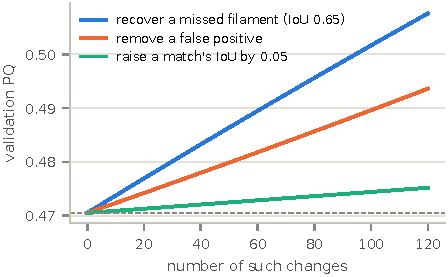
\includegraphics[width=0.66\textwidth]{figures/fig_leverage.pdf}
\caption{Validation PQ after $n$ changes of each kind, starting from the deployed model. Recovering
a missed filament is worth more than removing a false positive, and both are worth far more than
improving matches that already exist. \generatedby{book/make\_book\_figures.py:fig\_leverage}}
\label{fig:metric-leverage}
\end{figure}

\subsection{Why tuning a threshold rarely helps}\label{sec:metric-threshold}
Every model in this book outputs candidate masks with confidence scores, and a threshold decides
which candidates to keep. Lowering the threshold admits more candidates. Some of them become true
positives with a mean IoU of $q$, and the rest become false positives. If we admit $k$ correct and
$m$ incorrect candidates, the score changes to $(S+kq)/(D+\tfrac12k+\tfrac12m)$, which exceeds
$S/D$ if and only if
\begin{equation}
\frac{k}{k+m}>\frac{\PQ}{2q}.
\label{eq:metric-breakeven}
\end{equation}
In words, the precision of the newly admitted candidates must exceed $\PQ/(2q)$. With
$\PQ\approx0.46$ and $q\approx0.65$ this is about 35\%. At the optimal threshold, the
\emph{marginal} candidates sit at this break-even precision, so small moves of the threshold in
either direction change the score very little. In other words, PQ is flat near its optimum as a
function of the threshold. For example, in exp002 we swept seven thresholds and three minimum
areas, and the best setting in the whole grid was only $0.0022$ better than the default. We return
to Equation~\eqref{eq:metric-breakeven} in Chapter~\ref{ch:recall}, where it decides whether any
method for rescuing discarded candidates can possibly raise the score.

\section{How well do annotators agree?}\label{sec:metric-agreement}
The metric compares a model with the judgement of one person. How well do two people agree under
the same rule? We can measure this by treating one annotator's masks as ``predictions'' and scoring
them against another annotator's masks on the same photograph, for every ordered pair of
annotators. Over all 296 photographs with more than one annotator (\HumanPairs{} ordered pairs),
the result is $\PQ=\HumanPQAll{}$. On the validation photographs it is $\PQ=\HumanPQ{}$, with
$\SQ=\HumanSQ{}$ and $\RQ=\HumanRQ{}$
(\file{experiments/exp\_145\_host\_evaluation/src/annotator\_agreement.py}).

The final model scores \HostPQ{} against the same annotators, well above this value. Two
interpretations of this comparison are tempting, and both are wrong. The first is that the model is
better than the experts. It is not: a model trained on the labels of many annotators learns
something like their average, and an average lies closer to each individual than two individuals
lie to each other. This is a form of regression to the mean, and it does not indicate superhuman
skill. The second is that \HumanPQAll{} is a ceiling, so that nothing more can be gained. This is
also false. Each test photograph is scored against the annotator who labelled it, and a model can
match any single annotator better than another annotator does. The agreement between annotators
measures how uncertain the labels are; it does not bound the score.

A further experiment clarified the nature of the disagreement. If annotators were noisy
measurements of a single true outline, then combining two of them should predict a third better
than either one does alone, just as averaging several noisy measurements reduces their
error~\citep{galton1907}. On
the 151 photographs with three annotators, a consensus of two annotators predicted the held-out
third with a PQ of 0.3291, while a single other annotator did so with 0.3287. The consensus helped
by only 0.0004. The disagreement therefore appears to be \emph{structured}: annotators make
different decisions about where a faint extension stops belonging to a filament, and about whether
two nearby patches form one object or two. Such differences of judgement do not scatter at
random around a hidden true answer, so averaging does not remove them. The standard statistical
models of annotators, from the error-rate model of \citet{dawid1979} to STAPLE~\citep{warfield2004}
and the learning-from-crowds model of \citet{raykar2010}, assume a hidden true label of this kind.
Our measurement does not test those models directly, but it suggests that their central assumption
fits these labels poorly.

\section{How certain is a score?}\label{sec:metric-uncertainty}
A validation PQ of 0.4705 is a measurement on 106 photographs, and a different set of 106
photographs would have given a different value. The \keyterm{bootstrap}~\citep{efron1979,bootstrap} estimates
how different. We draw 106 photographs \emph{with replacement} from the validation set, recompute
the pooled PQ on this resampled set, and repeat the procedure 10,000 times. The spread of the
recomputed values approximates the sampling distribution of the score, and its 2.5th and 97.5th
percentiles form a 95\% \keyterm{percentile interval}.

The resampling unit must be the photograph and not the record. The records of one photograph share
a single set of predictions, so they are not independent, and resampling them separately would
pretend that the data contain more independent evidence than they do. Listing~\ref{lst:metric-bootstrap}
first sums the counts of each photograph and then resamples these sums.

\begin{lstlisting}[caption={Photograph-level bootstrap of pooled PQ. From \file{paper/make\_figures.py:bootstrap}.},label=lst:metric-bootstrap]
def pooled(sums):   # sums[..., :] = (sum of TP IoU, TP, FP, FN)
    iou, tp, fp, fn = sums[..., 0], sums[..., 1], sums[..., 2], sums[..., 3]
    denominator = tp + 0.5 * fp + 0.5 * fn
    return iou / denominator, iou / np.maximum(tp, 1), tp / denominator

def bootstrap(per_photo, draws=10000, seed=2026):
    rng = np.random.default_rng(seed)
    picks = rng.integers(0, len(per_photo), size=(draws, len(per_photo)))
    pq, sq, rq = pooled(per_photo[picks].sum(axis=1))
    return np.percentile(pq, [2.5, 97.5])
\end{lstlisting}

Figure~\ref{fig:metric-bootstrap} shows the result. The model's interval is \PQLow{}--\PQHigh{},
and the annotators' interval is \HumanPQLow{}--\HumanPQHigh{}, so the two do not overlap. The
model's interval is about 0.04 wide. This is a large number compared with the effects we usually
measured: most of the individual changes tested in this book moved validation PQ by less than 0.01,
well inside the interval. We dealt with this in two ways. We compared variants of a model on the
\emph{same} photographs, since most of the variation from photograph to photograph then cancels
out (Exercise~\ref{ex:metric-paired} makes this precise), and we treated small differences as noise
unless such a paired comparison showed otherwise.

\begin{figure}[t]
\centering
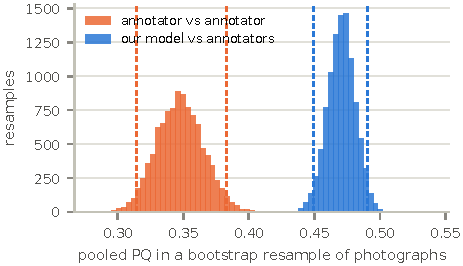
\includegraphics[width=0.66\textwidth]{figures/fig_bootstrap.pdf}
\caption{Bootstrap distributions of pooled PQ over 10,000 resamples of the validation photographs,
for the deployed model and for the agreement between annotators. Dashed lines mark the 95\%
percentile intervals. \generatedby{book/make\_book\_figures.py:fig\_bootstrap}}
\label{fig:metric-bootstrap}
\end{figure}

For a rate, such as the recall of filaments within a range of sizes, we use the \keyterm{Wilson
score interval}~\citep{wilson}. For $k$ successes in $n$ trials, with $\hat p=k/n$ and $z=1.96$, it
is
\begin{equation}
\frac{\hat p+\frac{z^2}{2n}}{1+\frac{z^2}{n}}\pm
\frac{z}{1+\frac{z^2}{n}}\sqrt{\frac{\hat p(1-\hat p)}{n}+\frac{z^2}{4n^2}} .
\end{equation}
Unlike the textbook interval $\hat p\pm z\sqrt{\hat p(1-\hat p)/n}$, the Wilson interval always
stays inside $[0,1]$ and behaves well when $n$ is small~\citep{agresti1998}.

\section{The organisers' implementation and ours}\label{sec:metric-code}
The organisers publish a self-evaluation notebook that contains their scoring code.
Listing~\ref{lst:metric-host} shows its core, and Listing~\ref{lst:metric-ours} shows our own
implementation. On the final model's validation predictions, the two return 0.4705249989 and
0.4705249990 respectively, with identical counts of true positives, false positives and false
negatives (exp145). They agree to nine decimal places.

\begin{lstlisting}[caption={The organisers' PQ, from their self-evaluation notebook (\file{experiments/exp\_145\_host\_evaluation/host/self\_evaluation\_notebook.ipynb}), lightly condensed.},label=lst:metric-host]
def get_pq_score(overlap_df):
    tp_iou_scores, fp_count, fn_count = [], 0, 0
    for row in overlap_df.itertuples(index=False):   # one row per annotator-image
        if row.n_gt == 0:
            fp_count += row.n_pred; continue
        if row.n_pred == 0:
            fn_count += row.n_gt; continue
        hit_matrix = row.iou_matrix > 0.5            # every pair above the threshold
        tp_iou_scores.extend(row.iou_matrix[hit_matrix].tolist())
        fp_count += int((hit_matrix.sum(dim=0) == 0).sum())   # predictions hitting nothing
        fn_count += int((hit_matrix.sum(dim=1) == 0).sum())   # annotations hit by nothing
    denominator = len(tp_iou_scores) + 0.5 * fp_count + 0.5 * fn_count
    return sum(tp_iou_scores) / denominator if denominator > 0 else 0.0
\end{lstlisting}

\begin{lstlisting}[caption={Our PQ for one record, and the pooling over records. Condensed from \file{shared/utils.py:compute\_pq} and \file{aggregate\_pq}.},label=lst:metric-ours]
def compute_pq(pred_masks, gt_masks, iou_threshold=0.5):
    ious = mask_util.iou(pred_rles, gt_rles, [0] * len(gt_rles))   # on RLE, in C
    matched_pred, matched_gt, iou_sum = set(), set(), 0.0
    pairs = np.argwhere(ious > iou_threshold)
    for i, j in sorted(pairs, key=lambda p: -ious[p[0], p[1]]):   # greedy, best first
        if i in matched_pred or j in matched_gt:
            continue
        matched_pred.add(i); matched_gt.add(j); iou_sum += ious[i, j]
    tp = len(matched_pred)
    return dict(tp=tp, fp=len(pred_masks) - tp, fn=len(gt_masks) - tp, iou_sum=iou_sum)

def aggregate_pq(per_record):
    tp = sum(r["tp"] for r in per_record); fp = sum(r["fp"] for r in per_record)
    fn = sum(r["fn"] for r in per_record); iou_sum = sum(r["iou_sum"] for r in per_record)
    return iou_sum / (tp + 0.5 * fp + 0.5 * fn)
\end{lstlisting}

There is one situation in which the two implementations disagree: two \emph{identical}
predictions placed over one annotation. The organisers' code counts two true positives, whereas ours
counts one true positive and one false positive. This case violates the premise of
Theorem~\ref{thm:metric-unique}, and since the scorer rejects overlapping submissions it can never
reach the leaderboard. We nevertheless pin it with a dedicated test
(\file{tests/test\_pq\_matches\_official.py}), so that the assumption remains visible to anyone who
changes the code.

\section*{Exercises}
\begin{exercise}{Uniqueness}
Construct two predictions that overlap each other and that both match the same annotation with an
IoU above one half. Which step in the proof of Theorem~\ref{thm:metric-unique} fails?
\end{exercise}

\begin{exercise}{RQ is $F_1$}
Show that RQ in Equation~\eqref{eq:metric-sqrq} equals the $F_1$ score of detection, and that
$\SQ\ge\tfrac12$ whenever $|\TP|>0$.
\end{exercise}

\begin{exercise}{Break-even precision}
Derive Equation~\eqref{eq:metric-breakeven}. Then show that when a model's threshold is optimal,
the precision of the marginal candidates equals $\PQ/(2q)$. What does this imply about the shape of
PQ as a function of the threshold near its maximum?
\end{exercise}

\begin{exercise}{Pooling versus averaging}
Using the final model's counts per record (recompute them with
\file{paper/make\_figures.py:record\_sums}), compare the pooled PQ with the mean of the per-record
PQ values and with the mean of the per-photograph PQ values. Which photographs cause the
differences?
\end{exercise}

\begin{exercise}{A paired bootstrap}\label{ex:metric-paired}
Suppose two models are scored on the same 106 photographs. Adapt Listing~\ref{lst:metric-bootstrap}
to bootstrap the \emph{difference} between their PQ values, resampling the photographs jointly for
both models. Show that the interval for the difference is much narrower than one would infer from
the two separate intervals, and explain why.
\end{exercise}

\chapter{Validation You Can Trust}\label{ch:validation}

\section{Introduction}\label{sec:val-why}
\epigraph{The first principle is that you must not fool yourself---and you are the easiest person
to fool.}{Richard Feynman, \emph{Cargo Cult Science} \citeyearpar{feynman1974}}

The public leaderboard may seem the obvious way to judge an idea, but it is a poor instrument for
day-to-day decisions. It accepts only five submissions a day. It scores only about half of the 180
test photographs, so its values are noisy. And it displays scores to two decimal places, so a model
that scores 0.405 and one that scores 0.414 both appear as 0.41. At one point we had four
quite different models whose validation scores spanned 0.013, and all four appeared on the
leaderboard as 0.36. Worse, a team that submits many variants and keeps whichever scores best
gradually fits the public half of the test set, which is a form of overfitting to a reused
holdout~\citep{dwork2015,blum2015}. Decisions must therefore be made on a \keyterm{validation split}: a set of
training photographs that we set aside and score locally, with the exact metric, as often as we
like.

This chapter is about making that split trustworthy, and about the many ways in which a validation
number can mislead. Section~\ref{sec:val-split} shows why the split must be made by photograph,
and Section~\ref{sec:val-time} discusses a subtler leak caused by the persistence of filaments over
time. Section~\ref{sec:val-transfer} measures how well validation scores predict the leaderboard.
Section~\ref{sec:val-oracles} introduces oracles, which measure the best result that an idea could
achieve before we spend effort building it, and Section~\ref{sec:val-traps} collects the
ways in which we misled ourselves with validation numbers during the project.

\section{Splitting by photograph}\label{sec:val-split}
The most obvious split, in which we shuffle the \AllRecords{} annotation records and hold out 15\%
of them, is wrong. A photograph labelled by three annotators appears as three records, and a random
split of the records would put some of them in the training set and others in the validation set.
The model would then be validated on photographs it had already seen during training, and its
validation score would be too high for a reason that has nothing to do with generalisation. Such
\keyterm{leakage} of information from the training data into the evaluation is a well-known fault
in applied machine learning~\citep{kaufman2012}.
Figure~\ref{fig:val-split} illustrates the difference.

\begin{figure}[t]
\centering
\begin{tikzpicture}[
  photo/.style={draw=inkmuted, fill=white, minimum width=0.62cm, minimum height=0.62cm, line width=0.6pt},
  rec/.style={circle, minimum size=0.2cm, inner sep=0pt, fill=#1},
  lab/.style={font=\sffamily\scriptsize, text=inksecondary}]
  % left: split by record
  \node[title] at (1.9,1.1) {split by record (leaks)};
  \foreach \i in {0,...,4} \node[photo] (a\i) at (\i*0.8,0) {};
  \foreach \i/\c in {0/vizblue,1/vizblue,2/vizorange,3/vizblue,4/vizorange}
    \node[rec=\c] at ($(a\i)+(-0.15,0.12)$) {};
  \foreach \i/\c in {0/vizorange,2/vizblue,3/vizblue}
    \node[rec=\c] at ($(a\i)+(0.15,0.12)$) {};
  \foreach \i/\c in {0/vizblue,3/vizorange}
    \node[rec=\c] at ($(a\i)+(0,-0.15)$) {};
  \node[lab, align=center] at (1.9,-0.85) {one photograph can feed\\ both training and validation};
  % right: split by photograph
  \begin{scope}[xshift=5.4cm]
    \node[title] at (1.9,1.1) {split by photograph (canonical)};
    \foreach \i in {0,...,4} \node[photo] (b\i) at (\i*0.8,0) {};
    \foreach \i/\c in {0/vizblue,1/vizblue,2/vizorange,3/vizblue,4/vizorange}
      \node[rec=\c] at ($(b\i)+(-0.15,0.12)$) {};
    \foreach \i/\c in {0/vizblue,2/vizorange,3/vizblue}
      \node[rec=\c] at ($(b\i)+(0.15,0.12)$) {};
    \foreach \i/\c in {0/vizblue,3/vizblue}
      \node[rec=\c] at ($(b\i)+(0,-0.15)$) {};
    \node[lab, align=center] at (1.9,-0.85) {every record follows\\ its photograph};
  \end{scope}
  \node[rec=vizblue] at (3.5,-1.65) {}; \node[lab, anchor=west] at (3.62,-1.65) {training record};
  \node[rec=vizorange] at (6.1,-1.65) {}; \node[lab, anchor=west] at (6.22,-1.65) {validation record};
\end{tikzpicture}
\caption{Squares are photographs and dots are their annotation records. Splitting the records at
random (left) puts records of one photograph on both sides of the split. Our canonical split
(right) assigns whole photographs. \drawnin{book/chapters/ch05\_validation.tex}}
\label{fig:val-split}
\end{figure}

Our canonical split, implemented in \file{shared/data\_split.py} and shown in
Listing~\ref{lst:val-split}, therefore assigns whole photographs to one side or the other. It also
\keyterm{stratifies} by GONG station, which means that it splits the photographs of each station
separately, so that both sides see the same mix of image quality. Finally, it uses a fixed random
seed, 2026, so that every experiment on every machine uses the same split. Changing the seed would
silently make every past comparison meaningless, so we treat it as a constant for the life of the
project.

\begin{lstlisting}[caption={The canonical split. From \file{shared/data\_split.py:make\_split}.},label=lst:val-split]
SPLIT_SEED = 2026   # fixed for the life of the project

def make_split(annotation_path, val_fraction=0.15, seed=SPLIT_SEED):
    stem_to_ids, _ = load_records(annotation_path)       # photograph -> its records
    by_site = defaultdict(list)
    for stem in sorted(stem_to_ids):
        by_site[instrument_of(stem)].append(stem)        # stratify by GONG station
    rng = np.random.default_rng(seed)
    train_stems, val_stems = [], []
    for site in sorted(by_site):
        stems = by_site[site]
        rng.shuffle(stems)
        n_val = max(1, round(len(stems) * val_fraction))
        val_stems.extend(stems[:n_val]); train_stems.extend(stems[n_val:])
    return Split(train_stems=sorted(train_stems), val_stems=sorted(val_stems),
                 train_image_ids=[i for s in sorted(train_stems) for i in stem_to_ids[s]],
                 val_image_ids=[i for s in sorted(val_stems) for i in stem_to_ids[s]])
\end{lstlisting}

The result is a training set of \TrainPhotos{} photographs with \TrainRecords{} records and
\TrainGT{} filaments, and a validation set of \ValPhotos{} photographs with \ValRecords{} records
and \ValGT{} filaments.

\section{Leakage through time}\label{sec:val-time}
Splitting by photograph removes the leak caused by duplicate records, but a subtler leak remains. A
filament survives on the disk for days or weeks, and GONG photographs the Sun around the clock from
six stations. Two photographs taken a day apart therefore usually show the same filaments, seen
through slightly different atmospheric conditions. If one of them is in the training set and the
other in the validation set, the model is partly validated on filaments it has already seen.
Figure~\ref{fig:val-temporal} shows how common this is: 43\% of the validation photographs have a
training photograph taken within one day of them, and 94\% have one within a week.

\begin{figure}[t]
\centering
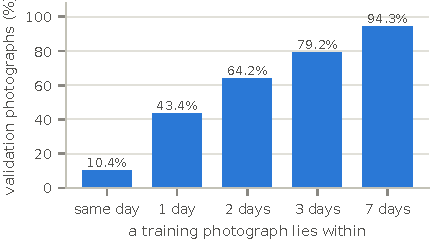
\includegraphics[width=0.62\textwidth]{figures/fig_temporal.pdf}
\caption{Fraction of validation photographs that have a training photograph within a given time
window, for the canonical split (from \file{docs/leaderboard-analysis.md}).
\generatedby{book/make\_book\_figures.py:fig\_temporal}}
\label{fig:val-temporal}
\end{figure}

We cannot fix this by removing training photographs close in time to each validation photograph,
because only 6 of the 106 validation photographs lie more than a week away from every training
photograph. The alternative, implemented in \file{shared/data\_split.py:make\_temporal\_split},
holds out five contiguous blocks of time spread across the years 2011--2022, and discards every
photograph within seven days of a block boundary. In this split no validation photograph has a
training photograph within a week, at the cost of 23 training photographs. Holding out blocks in
this way is the standard remedy for data with temporal or spatial structure~\citep{roberts2017}.

We nevertheless kept the canonical split for our main comparisons, for the following reason. When
we compare two variants of a model on the same split, such as a pipeline with and without erosion,
both variants benefit from the same leak, so their ranking remains valid. What the leak inflates is
the absolute value of the score. For absolute values, the leaderboard remained our reference
throughout the project.

\section{From validation to the leaderboard}\label{sec:val-transfer}
How well does a validation score predict the public score? Figure~\ref{fig:val-public} plots the
\ValPublicPoints{} submissions for which we recorded a validation score. Most of them follow a
simple rule: the public score is between 0.067 and 0.078 lower than the validation score. The
Mask2Former submissions lie at the top of this band or just above it. The deployed model scored
\FloatFortyPQ{} on validation and \BestPublic{} on the leaderboard, an offset of about 0.06.

\begin{figure}[t]
\centering
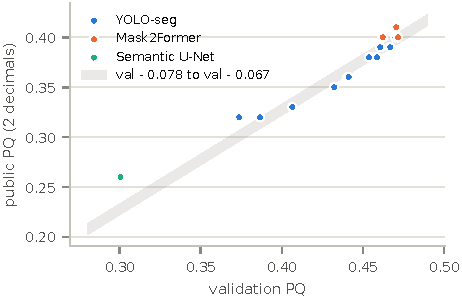
\includegraphics[width=0.66\textwidth]{figures/fig_val_public.pdf}
\caption{Validation PQ against public PQ for every submission whose description records its
validation score. The grey band marks the validation score minus 0.067 to 0.078.
\generatedby{book/make\_book\_figures.py:fig\_val\_public}}
\label{fig:val-public}
\end{figure}

\emph{Changes} in the score transfer less regularly than the scores themselves. The following
three changes had similar effects on validation but quite different effects on the leaderboard:
\begin{center}\small
\begin{tabular}{@{}lccc@{}}
\toprule
change & validation & public & fraction transferred \\
\midrule
inference at 2048 instead of 1280 & $+0.033$ & $+0.010$ & 30\% \\
one-pixel erosion of every mask & $+0.034$ & $+0.030$ & 88\% \\
a mask refiner (a deliberate regression) & $-0.008$ & $-0.010$ & 122\% \\
\bottomrule
\end{tabular}
\end{center}
These percentages must be read with care. Each public difference is the difference of two numbers
rounded to two decimal places, so a displayed change of $+0.010$ is consistent with any true change
between 0 and $+0.02$, and the 30\% in the first row could be anything from 0\% to 60\%. We never
established why the three changes transferred at different rates, and we do not speculate about it
here.

A weaker conclusion held up, and it turned out to be more useful. Every change that moved the
validation score by more than about 0.01 kept its sign on the leaderboard, whereas smaller changes
did not show up reliably. For example, the fine threshold sweep of exp057 scored 0.0028 above the
configuration that we later submitted as exp062, yet the two appeared on the leaderboard as 0.38
and 0.39 respectively. Similarly, exp082 added 77 masks to exp062, gaining 0.0035 on validation,
and appeared as 0.38. We therefore used the validation score as a \keyterm{gate} rather than as a
forecast. A change had to improve the validation score by a margin larger than its noise before it
earned a submission, and we accepted that the leaderboard might then disagree about the size of the
improvement.

The gate has a further limitation: it compares variants of \emph{one} family of models much better
than it compares different families. Our best YOLO ensemble and the deployed Mask2Former differed
by only 0.0024 on validation, yet the leaderboard separated them by 0.02. Conversely, a calibrated
ensemble of the two scored 0.001 higher than the Mask2Former alone on validation, but it appeared as
0.40 on the leaderboard against the Mask2Former's 0.41. When two different architectures tie on
validation, only a submission can separate them.

\subsection{Explanations we checked and rejected}\label{sec:val-rejected}
There are two textbook explanations for a gap between validation and test scores, and we measured
both. The first is that the test data differ from the training data, for example because they come
from other years or stations; in that case models would generalise worse to them. They do not
differ, as Figure~\ref{fig:data-years} shows. The second is a difference in weighting. Our
validation score counts a photograph once per annotator, and a photograph that three experts chose
to label might be easier than average. Reweighting the validation score so that each photograph
counts once changed it by only 0.0008.

What remains is ordinary generalisation error, together with the sampling noise that comes from
scoring half of 180 photographs. We also tested a third possibility with a deliberate probe: that
the test labels might be more inclusive than those of a single annotator, for example because they
were a consensus of several. We submitted a rule (exp028) that admitted many more candidates and
scored 0.041 \emph{worse} on validation. If the test labels had been more inclusive, it would have
scored well on the leaderboard; instead it scored 0.32, which is what the usual offset predicts.

\section{Measuring the ceiling before building}\label{sec:val-oracles}
Perhaps the most useful habit we developed was to ask, before building anything, how much an idea
could be worth at best. An \keyterm{oracle} answers this question by cheating: it uses the ground
truth to make the decision that the proposed method would have to make, and so it measures the best
result that any method of that kind could achieve. An oracle is never a submission; it is an upper
bound that tells us whether the idea is worth pursuing.

A testing manual that we adopted for the project turns this idea into a sequence of three steps,
which we applied most carefully in experiments exp113 to exp118.
\begin{enumerate}[leftmargin=*,itemsep=2pt]
\item \textbf{Ceiling.} Measure the largest gain in PQ that each family of repairs could achieve,
using an oracle. Discard the families whose ceiling is too small to matter.
\item \textbf{Operator.} Give the real repair operator a perfect trigger, which tells it, using the
ground truth, which instances to act on. Measure how much of the ceiling it recovers.
\item \textbf{Gate.} Only then build the real trigger that decides where to act, and measure the
precision it needs to break even.
\end{enumerate}
The order matters. If we reject an idea because its trigger failed, we have learned nothing about
the repair that the trigger was supposed to activate. We made this mistake at one point and later
corrected it, as we describe in Chapter~\ref{ch:post}.

A related discipline is \keyterm{pre-registration}.\footnote{Pre-registration is standard practice
in clinical trials and in experimental psychology, where it guards against choosing the hypothesis
after the data have been seen~\citep{nosek2018}.} Before spending money on a GPU run, we wrote down the hypothesis, the expected gain, and the result that would justify continuing or abandoning
the idea (\file{docs/PREREGISTRATION.md}). We then compared the outcome with numbers that had been
fixed in advance, instead of numbers chosen after seeing the result. The pre-registration written
before the final Mask2Former run, for example, recorded that the architecture had not yet been
tested properly, because the only previous attempt had been stopped long before its training
schedule finished (Section~\ref{sec:train-first}).

\section{Ways to fool ourselves}\label{sec:val-traps}
Each of the following errors occurred during the project, and each produced a validation number
that looked meaningful but was not.

\paragraph{Selecting on the validation set.} If we choose the best of eight configurations, or the
best of ten checkpoints, on the validation split, the score of the winner is optimistic, because
part of its advantage is luck. The deployed Mask2Former checkpoint was chosen in this way, and our
technical report says so. In another case (exp126) we observed a gain of 0.0028 that rested on four
predictions crossing the matching threshold, in the best of eight settings; we recorded it as noise.

\paragraph{Changing the unit of counting.} The validation split has 106 photographs but 180 records,
and a count made in one unit cannot be compared with a count made in the other
(Section~\ref{sec:metric-pooling}).

\paragraph{Changing the resolution.} In exp094 we found that scoring the masks of a model that works
on crops at the resolution of the crops, against a baseline scored at the native resolution, raised
the mean IoU by 0.012 with no model involved at all, because nearest-neighbour resampling happens to
round boundaries favourably. IoU should always be measured at the native resolution.

\paragraph{Comparing filtered and unfiltered populations.} SQ is an average over matched pairs only,
so it cannot be compared with a mean IoU computed over all instances
(Section~\ref{sec:metric-sq-properties}).

\paragraph{Quoting a downstream statistic as an upstream fact.} At one point our notes said that 284
missed filaments had ``zero overlap with any prediction''. This described the set of predictions
that remained \emph{after} the confidence threshold had been applied. In the full pool of candidate
masks, only 65 of those filaments had never been proposed at all
(Section~\ref{sec:recall-stages}).

\paragraph{Deploying something other than what was validated.} We once validated a fusion rule
with its second model run at a confidence floor of 0.05, and then prepared it for deployment with
that model run at a floor of 0.30. The deployed rule would have removed 312 candidates instead of a
handful. We caught the mistake because the deployment file had 979 rows, whereas the validated rule
predicted about 1,229.

The defence against the last error became a standard part of our pipeline. Every deployment path
replays its rule on the validation split, checks that it reproduces the validated score to within a
small tolerance, and checks a cheap invariant such as the number of rows before it writes a single
test prediction (Section~\ref{sec:sub-replay}).

\section*{Exercises}
\begin{exercise}{Leakage through records}
Split the records at random, holding out 15\%. How many validation records share their photograph
with a training record? Using the numbers of records per photograph from
Section~\ref{sec:data-magfilo}, estimate how strongly this leak could inflate a validation score.
\end{exercise}

\begin{exercise}{Temporal neighbours}
For each validation photograph, compute the time to the nearest training photograph, and reproduce
Figure~\ref{fig:val-temporal}. Then do the same for the temporal split in
\file{shared/data\_split.py}.
\end{exercise}

\begin{exercise}{Two decimal places}
Suppose that the public PQ equals the validation PQ minus 0.072, plus Gaussian noise with a standard
deviation of 0.01. Which validation score gives a 50\% chance of the leaderboard displaying 0.41?
Which gives a 90\% chance? How many submissions would you need to distinguish an
improvement of 0.005 from noise?
\end{exercise}

\begin{exercise}{An oracle}
Write an oracle that removes every false positive from the deployed model's validation predictions,
and compute the resulting PQ. Using Section~\ref{sec:metric-agreement}, explain why no real method
can reach it.
\end{exercise}

\chapter{Segmentation Paradigms and the First Baselines}\label{ch:paradigms}

\section{Introduction}\label{sec:paradigms-intro}
\epigraph{Essentially, all models are wrong, but some are useful.}{George Box and Norman Draper,
\emph{Empirical Model-Building and Response Surfaces} \citeyearpar[p.~424]{boxdraper1987}}

In this chapter we describe our first models. Before doing so, we need some vocabulary, because
computer vision distinguishes several kinds of segmentation, and the differences between them
turn out to be central to this problem. Section~\ref{sec:paradigms-kinds} defines semantic,
instance and panoptic segmentation. Sections~\ref{sec:paradigms-unet}--\ref{sec:paradigms-cc}
describe the simplest approach, in which a network labels each pixel as filament or background
and a separate rule then divides the filament pixels into objects. Section~\ref{sec:paradigms-results}
reports how well this approach worked, and Section~\ref{sec:paradigms-fragments} describes two
attempts to improve the rule that divides pixels into objects. Section~\ref{sec:paradigms-stop}
explains why we moved on to models that output objects directly, and
Section~\ref{sec:paradigms-decoders} surveys the three main families of such models.

\section{Semantic, instance and panoptic segmentation}\label{sec:paradigms-kinds}
Computer vision has three standard ways to say which pixels of an image belong to filaments. They
differ in what they say about \emph{identity}, that is, about which filament each pixel belongs to.

A \keyterm{semantic segmentation} assigns a class to every pixel. With a single class of interest,
it is a function from the image to a map of probabilities,
\begin{equation}
f_\theta : \R^{H\times W} \to [0,1]^{H\times W}, \qquad
f_\theta(\mathbf{x})_i = \Pr(\text{pixel } i \text{ is filament} \mid \mathbf{x}),
\label{eq:par-semantic}
\end{equation}
where $\mathbf{x}$ is the photograph and $\theta$ are the weights of the network. The map says
nothing about identity. Two filaments that touch become a single blob, and a single filament that
is interrupted by a faint stretch becomes two separate pieces.

An \keyterm{instance segmentation} returns a set of objects,
\begin{equation}
\{(m_k, s_k)\}_{k=1}^{K}, \qquad m_k \in \{0,1\}^{H\times W}, \quad s_k \in [0,1],
\label{eq:par-instance}
\end{equation}
consisting of a binary mask $m_k$ and a confidence score $s_k$ for each object. Identity is now
part of the answer. In general-purpose benchmarks such as COCO~\citep{coco}, the masks of two
instances are allowed to overlap.

A \keyterm{panoptic segmentation}~\citep{pq} gives every pixel exactly one owner, which is either
a ``stuff'' class, such as sky or road, or one particular instance of a ``thing'' class, such as a
car. Our competition is a panoptic problem with a single thing class: the background is the only
stuff, and each filament is a thing. The rule that no pixel may belong to two masks is the panoptic
constraint, and it is the reason why the metric is called Panoptic Quality.

\begin{figure}[t]
\centering
\begin{tikzpicture}[
  panel/.style={draw=inkmuted, line width=0.6pt, fill=gridline!45, minimum width=3.3cm,
                minimum height=2.45cm, rounded corners=2pt},
  fil/.style={line width=5.5pt, line cap=round, draw=#1}]
  \foreach \px/\name/\what in {0/semantic/{one map: is this\\ pixel a filament?},
                               3.9/instance/{one mask per object;\\ masks may overlap},
                               7.8/panoptic/{every pixel has\\ exactly one owner}}{
    \node[panel] at (\px,0) {};
    \node[title] at (\px,1.5) {\name};
    \node[note] at (\px,-1.62) {\what};
  }
  % semantic: one class; the two lower filaments touch and fuse
  \draw[fil=vizblue!75] (-1.25,0.62) .. controls (-0.6,0.95) and (0.2,0.3) .. (1.2,0.7);
  \draw[fil=vizblue!75] (-1.2,-0.35) .. controls (-0.7,-0.8) and (-0.1,-0.2) .. (0.45,-0.75);
  \draw[fil=vizblue!75] (0.2,-0.52) .. controls (0.55,-0.3) and (0.95,-0.45) .. (1.3,-0.1);
  % instance: one colour per object, translucent so the overlap shows
  \begin{scope}[xshift=3.9cm]
    \draw[fil=vizblue, draw opacity=0.7] (-1.25,0.62) .. controls (-0.6,0.95) and (0.2,0.3) .. (1.2,0.7);
    \draw[fil=vizorange, draw opacity=0.7] (-1.2,-0.35) .. controls (-0.7,-0.8) and (-0.1,-0.2) .. (0.45,-0.75);
    \draw[fil=vizaqua, draw opacity=0.7] (0.2,-0.52) .. controls (0.55,-0.3) and (0.95,-0.45) .. (1.3,-0.1);
    \draw[->, line width=0.5pt, draw=inkprimary] (0.75,-0.95) -- (0.3,-0.62);
    \node[note, anchor=west] at (0.62,-1.0) {overlap};
  \end{scope}
  % panoptic: opaque, lowest score painted first so the highest score owns contested pixels
  \begin{scope}[xshift=7.8cm]
    \draw[fil=vizaqua] (0.2,-0.52) .. controls (0.55,-0.3) and (0.95,-0.45) .. (1.3,-0.1);
    \draw[fil=vizorange] (-1.2,-0.35) .. controls (-0.7,-0.8) and (-0.1,-0.2) .. (0.45,-0.75);
    \draw[fil=vizblue] (-1.25,0.62) .. controls (-0.6,0.95) and (0.2,0.3) .. (1.2,0.7);
  \end{scope}
\end{tikzpicture}
\caption{The same three filaments as a semantic map, as instances and as a panoptic segmentation.
In the semantic map the two lower filaments touch and fuse into one blob. As instances they are
separate, but their masks overlap. The panoptic answer gives the contested pixels to one mask, here
the orange one, which has the higher score (Section~\ref{sec:masks-paint}).
\drawnin{book/chapters/ch06\_paradigms.tex}}
\label{fig:par-kinds}
\end{figure}

Figure~\ref{fig:par-kinds} shows the three kinds of answer for the same three filaments. To turn a
semantic answer into a panoptic one we must make two additional decisions: how to divide the
foreground pixels into objects, and who owns a pixel that two objects both claim. The second
decision is made by painting, which we described in Section~\ref{sec:masks-paint}. The rest of this
chapter is about the first decision, and about our first models, which made it after the network
had finished its work.

\section{An encoder--decoder for dense prediction}\label{sec:paradigms-unet}
Our first model (exp001) was a semantic segmentation model. This is the natural first attempt:
semantic segmentation is the most thoroughly studied problem in the field, and its output, a
probability for every pixel, is easy to inspect and to debug.

\subsection{The U-Net}\label{sec:par-unet-arch}
The \keyterm{U-Net}~\citep{unet}, a refinement of the fully convolutional network
of \citet{long2015}, is the standard architecture for dense prediction when the structures of
interest are small compared with the image. Figure~\ref{fig:par-unet} shows its
shape. The \keyterm{encoder} is an ordinary image classifier, such as a ResNet~\citep{resnet} or an
EfficientNet~\citep{efficientnet}, with its final classification layer removed. Each stage of the
encoder halves the height and width of its feature map and increases the number of channels. The
deep features therefore summarise a large part of the image, but they locate things only coarsely:
at the bottom of a typical encoder, one feature vector describes a block of $32\times32$ pixels.

The \keyterm{decoder} reverses the process. Each decoder stage doubles the resolution and then
\emph{concatenates} the encoder's feature map of the same size, carried across by a
\keyterm{skip connection}, before applying further convolutions. A final $1\times1$ convolution
produces one number $z_i$ for each pixel $i$, called a \keyterm{logit}, and the sigmoid function
turns it into a probability,
\begin{equation}
p_i = \sigmoid(z_i) = \frac{1}{1+e^{-z_i}}.
\end{equation}

The skip connections are what make this architecture suitable for filaments. The deep path of the
network can answer the question ``is there a filament somewhere around here?'' using a wide
context, while the skip connections answer the question ``which pixels, precisely?'' using features
computed before the resolution was reduced. A filament needs both answers. Its shape can extend
over hundreds of pixels, but its body is often only four or five pixels wide, and a structure that
narrow does not survive to the bottom of the encoder.

\begin{figure}[t]
\centering
\begin{tikzpicture}[
  fmap/.style={draw=#1!80!black, fill=#1!22, line width=0.5pt, inner sep=0pt},
  skipflow/.style={->, line width=0.7pt, draw=vizaqua!75!black, dashed},
  udflow/.style={->, line width=0.8pt, draw=inksecondary}]
  \node[inner sep=0pt] (in) at (-1.6,0) {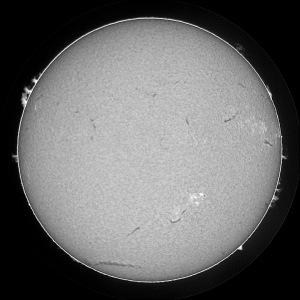
\includegraphics[width=1.25cm]{figures/thumb_input.png}};
  \node[note, below=2pt of in] {photograph};
  % encoder: resolution falls, channels grow
  \node[fmap=vizblue, minimum width=0.22cm, minimum height=1.8cm] (e0) at (0,0) {};
  \node[fmap=vizblue, minimum width=0.34cm, minimum height=1.2cm] (e1) at (0.9,-2.0) {};
  \node[fmap=vizblue, minimum width=0.50cm, minimum height=0.8cm] (e2) at (1.8,-3.6) {};
  \node[fmap=vizviolet, minimum width=0.72cm, minimum height=0.5cm] (b) at (3.7,-4.8) {};
  % decoder: resolution returns
  \node[fmap=vizorange, minimum width=0.50cm, minimum height=0.8cm] (d2) at (5.6,-3.6) {};
  \node[fmap=vizorange, minimum width=0.34cm, minimum height=1.2cm] (d1) at (6.5,-2.0) {};
  \node[fmap=vizorange, minimum width=0.22cm, minimum height=1.8cm] (d0) at (7.4,0) {};
  \node[box=vizorange, right=0.45cm of d0, text width=1.9cm] (out) {one logit per pixel\\ $p_i=\sigmoid(z_i)$};
  \draw[udflow] (in) -- (e0);
  \draw[udflow] (e0.south) -- node[note, left=2pt] {halve} (e1.north);
  \draw[udflow] (e1.south) -- node[note, left=2pt] {halve} (e2.north);
  \draw[udflow] (e2.south) |- (b.west);
  \draw[udflow] (b.east) -| (d2.south);
  \draw[udflow] (d2.north) -- node[note, right=2pt] {double} (d1.south);
  \draw[udflow] (d1.north) -- node[note, right=2pt] {double} (d0.south);
  \draw[udflow] (d0) -- (out);
  \draw[skipflow] (e0.east) -- node[note, above=1pt] {skip: copy and concatenate} (d0.west);
  \draw[skipflow] (e1.east) -- (d1.west);
  \draw[skipflow] (e2.east) -- (d2.west);
  \node[note, anchor=east] at (-0.25,-2.0) {1/2};
  \node[note, anchor=east] at (0.65,-3.6) {1/4};
  \node[note] at (3.7,-5.35) {bottleneck: 1/8 here, 1/32 in real encoders};
  \node[title, text=vizblue!80!black] at (0.2,1.25) {encoder};
  \node[title, text=vizorange!80!black] at (7.2,1.25) {decoder};
\end{tikzpicture}
\caption{A U-Net. The heights of the bars stand for spatial resolution and their widths for the
number of channels. The encoder halves the resolution at each stage; the decoder doubles it again
and concatenates the encoder's map of the same size (dashed skip connections). Real encoders use
five halvings, whereas the diagram shows three. \drawnin{book/chapters/ch06\_paradigms.tex}}
\label{fig:par-unet}
\end{figure}

\subsection{Our first model}\label{sec:par-exp001}
Experiment exp001 used \keyterm{U-Net++}~\citep{unetpp}, a variant of the U-Net in which each skip
connection passes through a small stack of nested convolution blocks, so that the encoder features
and the decoder features are more alike when they are joined. The encoder was an EfficientNet-B4
pretrained on ImageNet~\citep{deng2009}. The photographs are grey, whereas an ImageNet encoder
expects three colour channels, so we copied the grey image into all three. Each image was first
contrast-equalised with CLAHE~\citep{zuiderveld1994} (contrast-limited adaptive histogram
equalisation, with a clip limit of 2.0 on an $8\times8$
grid of tiles) and then blurred very slightly (a Gaussian with $\sigma=0.7$ pixels). The model was
trained on $512\times512$ inputs with batches of 8, a learning rate of $10^{-4}$ with a two-epoch
warm-up and a cosine decay~\citep{sgdr}, and mixed-precision arithmetic~\citep{mixedprecision} on
a T4 GPU. Early stopping ended
training at epoch 46; the best epoch was epoch 34.

\subsection{Example: the cost of resolution, measured before training}\label{sec:par-ceiling}
An input of $512\times512$ pixels is a quarter of the native width, so a filament four pixels wide
becomes one pixel wide. What is the best score that a model working at this resolution could
achieve? We answered this question before training anything, using a kind of measurement
that later became a habit (Section~\ref{sec:val-oracles}). We took the \emph{annotated} filament
masks and shrank their union to the training resolution, in the same way that the training targets
were built. We then thresholded the result, enlarged it back to $2048\times2048$ pixels, split it
into connected components (Section~\ref{sec:paradigms-cc}), and scored these components with PQ.
The result is the output of a \emph{perfect} semantic model at that resolution, so its score is an
upper bound on what the design can achieve:
\begin{center}\small
\begin{tabular}{@{}ccccc@{}}
\toprule
resolution & closing kernel & PQ & SQ & RQ \\
\midrule
512 & none & \textbf{0.7642} & 0.7660 & 0.9977 \\
512 & 5 px & 0.7589 & 0.7607 & 0.9977 \\
512 & 9 px & 0.7481 & 0.7508 & 0.9965 \\
1024 & none & \textbf{0.8692} & 0.8702 & 0.9988 \\
1024 & 5 px & 0.8430 & 0.8449 & 0.9977 \\
\bottomrule
\end{tabular}
\end{center}

We drew three conclusions from this table, and each of them changed a decision. First, connected
components recover the filaments almost perfectly from a perfect mask (RQ is 0.998), so separating
the filaments from each other is not difficult \emph{when the mask is correct}. Second, all of the
loss is in SQ: shrinking the image blurs every boundary, which costs about a quarter of the IoU at
512 pixels and about an eighth at 1024. Third, morphological \emph{closing}~\citep{serra1982} (a dilation followed
by an erosion, which rejoins nearby fragments) makes matters worse, because it widens every mask by
more than the rejoined fragments are worth. We therefore switched closing off.

\section{Losses for imbalanced segmentation}\label{sec:par-loss}
Filament pixels make up about one percent of the pixels on the disk. This \keyterm{class
imbalance} causes problems for the standard loss function. Plain binary cross-entropy is already
99\% ``correct'' for a network that predicts background everywhere, so it gives weak and misleading
gradients early in training. In exp001 we combined two standard remedies.

The first is a \keyterm{weighted binary cross-entropy}, which makes a missed filament pixel $w$
times as costly as a false one:
\begin{equation}
\mathcal{L}_{\mathrm{BCE}} = -\frac{1}{N}\sum_{i=1}^{N}\Big[\,w\,y_i\log p_i + (1-y_i)\log(1-p_i)\Big],
\qquad w = 8,
\label{eq:par-bce}
\end{equation}
where $y_i\in\{0,1\}$ is the target for pixel $i$ and $N$ is the number of pixels.

The second is the \keyterm{soft Dice loss}~\citep{vnet}, which replaces the counts in the Dice coefficient of
Section~\ref{sec:masks-iou} with probabilities, so that it can be differentiated:
\begin{equation}
\mathcal{L}_{\mathrm{Dice}} = 1 - \frac{2\sum_i p_i y_i + \epsilon}{\sum_i p_i + \sum_i y_i + \epsilon},
\qquad \epsilon = 1.
\label{eq:par-dice}
\end{equation}
The Dice coefficient measures overlap relative to the size of the objects, so the very large number
of easy background pixels cannot dominate it~\citep{sudre2017}. We can see this by computing its gradient. Write
$I=\sum_i p_i y_i$ for the soft intersection and $S=\sum_i p_i+\sum_i y_i+\epsilon$. Then
\begin{equation}
\frac{\partial\mathcal{L}_{\mathrm{Dice}}}{\partial p_i} = \frac{(2I+\epsilon) - 2y_iS}{S^2}.
\end{equation}
For a background pixel ($y_i=0$) the gradient is positive, so gradient descent lowers $p_i$. For a
filament pixel ($y_i=1$) it is negative, since $I$ can exceed neither $\sum_i p_i$ nor $\sum_i y_i$,
so that $2I+\epsilon\le S<2S$; gradient descent therefore raises $p_i$. The quantities $I$ and
$S$ measure the soft predicted foreground and the annotated foreground, and neither of them grows
with the number of correctly classified background pixels, so the gradients do not shrink when the
objects occupy only a small part of the image. The smoothing
constant $\epsilon$ prevents the expression $0/0$ on an image that contains no filament. The total
loss was the average of the two terms, $\mathcal{L}=\tfrac12\mathcal{L}_{\mathrm{BCE}}+\tfrac12
\mathcal{L}_{\mathrm{Dice}}$, as Listing~\ref{lst:par-loss} shows.

\begin{lstlisting}[caption={Weighted cross-entropy plus soft Dice. Condensed from
\file{experiments/exp\_001\_baseline/src/model.py}.},label=lst:par-loss]
class CombinedLoss(nn.Module):
    def __init__(self, bce_weight=0.5, dice_weight=0.5, pos_weight=8.0):
        super().__init__()
        self.bce_weight, self.dice_weight = bce_weight, dice_weight
        self.bce = nn.BCEWithLogitsLoss(pos_weight=torch.tensor(pos_weight))

    def forward(self, logits, targets):            # both (batch, 1, H, W)
        bce = self.bce(logits, targets)
        probs = torch.sigmoid(logits)
        intersection = (probs * targets).sum((2, 3))
        cardinality = probs.sum((2, 3)) + targets.sum((2, 3))
        # +1 keeps an image with no filament from giving 0/0
        dice = 1.0 - ((2.0 * intersection + 1.0) / (cardinality + 1.0)).mean()
        return self.bce_weight * bce + self.dice_weight * dice
\end{lstlisting}

\section{From probabilities to instances}\label{sec:paradigms-cc}
A probability map is not yet a submission. In exp001 we turned it into instances with the simplest
possible rule, summarised in Algorithm~\ref{alg:par-cc}.

\begin{algorithmblock}{From a probability map to disjoint instances (exp001)\label{alg:par-cc}}
\item \textbf{input:} a $512\times512$ probability map $P$; threshold $\tau=0.5$; minimum area $a_{\min}=150$
\item enlarge $P$ to $2048\times2048$ by bilinear interpolation;
\item $B\leftarrow[\,P\ge\tau\,]$, a binary mask;
\item (optionally) close small gaps in $B$; this step was switched off;
\item remove every pixel of $B$ that lies outside the solar disk;
\item label the 8-connected components of $B$;
\item \textbf{return} the components whose area is at least $a_{\min}$, largest first
\end{algorithmblock}

Two details deserve comment. The map is enlarged \emph{before} it is thresholded, because enlarging
a thresholded map would turn every smooth edge into a staircase. The minimum area of 150 pixels
removes specks; the smallest one percent of annotated filaments cover about 208 pixels, so very few
real filaments are that small.

Two foreground pixels belong to the same \keyterm{connected component} if they can be joined by a
path of foreground pixels~\citep{rosenfeld1966}. With \keyterm{8-connectivity}, each step of such a path may go to any of
the eight neighbouring pixels, including the diagonal ones; with 4-connectivity, only to the four
that share an edge. Figure~\ref{fig:par-cc} works through a small example. Since the connected
components partition the foreground, the resulting masks are automatically disjoint, and no
painting step is needed.

\begin{figure}[t]
\centering
\begin{tikzpicture}[pcell/.style={minimum size=0.27cm, inner sep=0pt, draw=white, line width=0.4pt}]
  % panel 1: probabilities in tenths
  \foreach \row [count=\y from 0] in {{0,1,1,0,0,0,0,0,0,0},{1,7,8,6,2,0,0,0,1,0},
      {0,2,6,8,4,7,8,1,0,0},{0,0,1,2,1,2,9,8,2,0},{0,0,0,0,0,1,7,9,6,1},{0,0,0,0,0,0,1,2,1,0}}{
    \foreach \p [count=\x from 0] in \row {
      \pgfmathtruncatemacro{\shade}{\p*10}
      \node[pcell, fill=vizblue!\shade!white] at (\x*0.27, -\y*0.27)
        {\tiny\sffamily\ifnum\p>6 \color{white}\else\color{inksecondary}\fi\p};
    }
  }
  % panel 2: threshold at 0.5
  \begin{scope}[xshift=3.7cm]
  \foreach \row [count=\y from 0] in {{0,1,1,0,0,0,0,0,0,0},{1,7,8,6,2,0,0,0,1,0},
      {0,2,6,8,4,7,8,1,0,0},{0,0,1,2,1,2,9,8,2,0},{0,0,0,0,0,1,7,9,6,1},{0,0,0,0,0,0,1,2,1,0}}{
    \foreach \p [count=\x from 0] in \row {
      \ifnum\p>4 \node[pcell, fill=inkprimary!75] at (\x*0.27, -\y*0.27) {};
      \else \node[pcell, fill=gridline!60] at (\x*0.27, -\y*0.27) {}; \fi
    }
  }
  \end{scope}
  % panel 3: component labels
  \begin{scope}[xshift=7.4cm]
  \foreach \row [count=\y from 0] in {{0,0,0,0,0,0,0,0,0,0},{0,1,1,1,0,0,0,0,0,0},
      {0,0,1,1,0,2,2,0,0,0},{0,0,0,0,0,0,2,2,0,0},{0,0,0,0,0,0,2,2,2,0},{0,0,0,0,0,0,0,0,0,0}}{
    \foreach \cl [count=\x from 0] in \row {
      \ifcase\cl \node[pcell, fill=gridline!60] at (\x*0.27, -\y*0.27) {};
      \or \node[pcell, fill=vizblue] at (\x*0.27, -\y*0.27) {};
      \or \node[pcell, fill=vizorange] at (\x*0.27, -\y*0.27) {}; \fi
    }
  }
  \end{scope}
  \node[title] at (1.215,0.45) {probability, in tenths};
  \node[title] at (4.915,0.45) {threshold at 0.5};
  \node[title] at (8.615,0.45) {8-connected components};
  \draw[flow] (2.75,-0.675) -- (3.55,-0.675);
  \draw[flow] (6.45,-0.675) -- (7.25,-0.675);
  \draw[vizorange, line width=1.1pt] (0.945,-0.675) rectangle (1.215,-0.405);
  \node[note] at (1.215,-1.8) {outlined: 0.4, just below the threshold};
\end{tikzpicture}
\caption{Connected-component labelling of a small probability map. One faint pixel (0.4) lies
below the threshold, so what may be a single filament becomes two components, shown in blue and
orange. If both halves belong to one annotated filament, each covers only part of it; if neither
half reaches an IoU of 0.5 with the filament, PQ counts two false positives and one false negative.
\drawnin{book/chapters/ch06\_paradigms.tex}}
\label{fig:par-cc}
\end{figure}

Listing~\ref{lst:par-cc} gives the implementation, using OpenCV's connected-component labelling.

\begin{lstlisting}[caption={Semantic probabilities to disjoint instances. Condensed from
\file{experiments/exp\_001\_baseline/src/postprocess.py}.},label=lst:par-cc]
def probability_to_instances(probability, threshold, min_area, closing_kernel, disk=None):
    # 1. enlarge to the native frame BEFORE thresholding, or every edge becomes a staircase
    upsampled = cv2.resize(probability.astype(np.float32), (2048, 2048),
                           interpolation=cv2.INTER_LINEAR)
    binary = (upsampled >= threshold).astype(np.uint8)            # 2. threshold
    if closing_kernel > 1:                                         # 3. optional closing
        kernel = cv2.getStructuringElement(cv2.MORPH_ELLIPSE, (closing_kernel, closing_kernel))
        binary = cv2.morphologyEx(binary, cv2.MORPH_CLOSE, kernel)
    if disk is not None:                                           # 4. nothing off the disk
        binary &= disk.mask(binary.shape)
    n, labels, stats, _ = cv2.connectedComponentsWithStats(binary, connectivity=8)
    instances = [(stats[k, cv2.CC_STAT_AREA], (labels == k).astype(np.uint8))
                 for k in range(1, n) if stats[k, cv2.CC_STAT_AREA] >= min_area]
    instances.sort(key=lambda item: -item[0])                      # 5. largest first
    return [mask for _, mask in instances]
\end{lstlisting}

\section{Results of the dense models}\label{sec:paradigms-results}
Our first model, exp001, scored a PQ of 0.2957 on the 180 validation records and 0.26 on the public
leaderboard. The components of its score are more informative than the total:
\begin{center}\small
\setlength{\tabcolsep}{4pt}
\begin{tabular}{@{}lccccc@{}}
\toprule
model & PQ & SQ & RQ & TP / FP / FN & instances per image \\
\midrule
exp001 (U-Net++, 512) & 0.2957 & 0.629 & 0.470 & 673 / 866 / 652 & 8.6 (annotations: 7.4) \\
\bottomrule
\end{tabular}
\end{center}
The matched masks were reasonable, with a mean IoU of 0.63, but recognition was poor. Fewer than
half of the predictions, and only about half of the annotated filaments, found a partner. The model
was not failing wholesale: only 4 of the 180 records scored zero, so it was doing something useful
on almost every photograph.

Our second dense model, exp004, removed the two most obvious limitations of the first. It trained a
U-Net with a ResNet-34 encoder at twice the resolution, $1024\times1024$, for 300 epochs, until the
validation loss had stopped improving for many epochs. It ran on the eight cores of a Kaggle TPU in
3.8 hours (Appendix~\ref{app:infra}), and at test time it averaged the probability maps predicted
for flipped copies of the image. It scored 0.28 on the public leaderboard, an improvement of only
two hundredths for four times as many pixels and a fully converged model. It also emitted 9.50
instances per image, against 7.4 in the annotations.

\section{Grouping pixels by other means}\label{sec:paradigms-fragments}
Our first explanation for the poor recognition of exp001 was \keyterm{fragmentation}. A filament
that the seeing conditions break into several dark patches is a single object to the annotator, but
connected components cannot know that, so they return one instance per patch, as in
Figure~\ref{fig:par-cc}. Each patch covers only part of the filament, so none of them reaches an IoU
of 0.5, and one physical error becomes one false negative plus several false positives. This
explanation is plausible, and it makes a testable prediction: the model should emit many more
instances than there are filaments.

It turned out that it did not. The model emitted 8.6 instances per image against 7.4 in the
annotations, a ratio of 1.16, which indicates at most a mild over-segmentation.
 We had promoted the explanation to a finding without testing it. Before we noticed
this, we had designed two decoders to fix the supposed problem. We describe them next, together
with the tests that we used to evaluate them.

\subsection{Seeding instances on spines}\label{sec:par-spine}
Every one of the \AllFilaments{} annotations includes a spine, a polyline along the filament's axis
(Section~\ref{sec:data-spines}). Our plan for exp004 was to exploit this. Even when a filament is
broken into patches, it has a single spine. We would therefore predict the spine as a second output
channel of the network, treat each connected piece of the predicted spine as one filament, and give
every pixel of the mask to its nearest spine. This assignment is a \keyterm{Voronoi partition} of
the mask, and it can be computed in a single pass by a distance transform that also reports
\emph{which} seed pixel is nearest to each pixel. Listing~\ref{lst:par-spine} shows the
implementation.

\begin{lstlisting}[caption={Spine-seeded instances. Condensed from
\file{experiments/exp\_004\_spine\_tpu/src/decompose.py}.},label=lst:par-spine]
def decompose(mask, spine, min_area=150, min_spine_area=8):
    spine = ((spine > 0) & (mask > 0)).astype(np.uint8)        # spines inside the mask only
    n, spine_labels, stats, _ = cv2.connectedComponentsWithStats(spine, connectivity=8)
    keep = [k for k in range(1, n) if stats[k, cv2.CC_STAT_AREA] >= min_spine_area]
    if not keep:
        return connected_components(mask, min_area)            # fall back to exp001
    seeds = np.zeros_like(spine_labels, dtype=np.int32)
    for new, old in enumerate(keep, start=1):
        seeds[spine_labels == old] = new
    # For every non-seed pixel: the index of its nearest seed pixel (straight-line distance).
    _, index = cv2.distanceTransformWithLabels((seeds == 0).astype(np.uint8), cv2.DIST_L2, 3,
                                               labelType=cv2.DIST_LABEL_PIXEL)
    lookup = np.concatenate([[0], seeds.reshape(-1)[np.flatnonzero(seeds)]])
    assigned = np.where(mask > 0, lookup[index], 0)             # seed index -> spine label
    return [m for m in ((assigned == k).astype(np.uint8) for k in range(1, len(keep) + 1))
            if m.sum() >= min_area]
\end{lstlisting}

\begin{figure}[t]
\centering
\begin{tikzpicture}[
  piece/.style={line width=6pt, line cap=round, draw=#1},
  spn/.style={line width=0.8pt, draw=inkprimary, dash pattern=on 2.2pt off 1.4pt}]
  \foreach \sx/\lab in {0/{(a) mask and predicted spines}, 3.9/{(b) connected components: one}, 7.8/{(c) spine seeding: two}}{
    \node[note] at (\sx+1.3,-1.25) {\lab};
  }
  % (a) the union mask in grey with both spines
  \draw[piece=inkmuted!55] (0,0) .. controls (0.6,0.45) and (1.2,0.45) .. (1.7,0.05);
  \draw[piece=inkmuted!55] (1.45,0.2) .. controls (1.8,-0.2) and (2.2,-0.6) .. (2.65,-0.75);
  \draw[spn] (0,0) .. controls (0.6,0.45) and (1.2,0.45) .. (1.7,0.05);
  \draw[spn] (1.45,0.2) .. controls (1.8,-0.2) and (2.2,-0.6) .. (2.65,-0.75);
  % (b) connected components: the touching filaments form one component
  \begin{scope}[xshift=3.9cm]
    \draw[piece=vizblue] (0,0) .. controls (0.6,0.45) and (1.2,0.45) .. (1.7,0.05);
    \draw[piece=vizblue] (1.45,0.2) .. controls (1.8,-0.2) and (2.2,-0.6) .. (2.65,-0.75);
  \end{scope}
  % (c) spine seeding: each pixel goes to its nearest spine
  \begin{scope}[xshift=7.8cm]
    \draw[piece=vizorange] (1.45,0.2) .. controls (1.8,-0.2) and (2.2,-0.6) .. (2.65,-0.75);
    \draw[piece=vizblue] (0,0) .. controls (0.6,0.45) and (1.2,0.45) .. (1.7,0.05);
  \end{scope}
\end{tikzpicture}
\caption{What spine seeding can do. Two filaments touch, so their union forms one connected
component (b). Their spines are separate, so assigning each pixel to its nearest spine divides the
mask into two instances (c). Rejoining the patches of a broken filament is harder, because the
spine is first cut to the mask, so a gap that severs the mask also severs its spine.
\drawnin{book/chapters/ch06\_paradigms.tex}}
\label{fig:par-spine}
\end{figure}

The first line of Listing~\ref{lst:par-spine} contains a detail that the design description did
not mention. It intersects the spine with the mask, so a gap that cuts the mask in two also cuts the
spine in two, and each patch keeps its own seed. A patch is rejoined to its neighbour only when it
contains fewer than 8 spine pixels of its own. The method therefore \emph{separates} two touching
filaments with distinct spines reliably (Figure~\ref{fig:par-spine}), but it rejoins the pieces of
a broken filament only occasionally.

Before we spent any TPU time on the idea, we tested it without training a model. The test took the
annotated masks, imitated fragmentation by eroding them and then dilating them with a $k\times k$
square (which severs thin necks), and scored both decoders against the true instances on 60
validation records:
\begin{center}\small
\begin{tabular}{@{}ccccc@{}}
\toprule
erosion $k$ & predicted / true instances & components PQ & spine PQ & difference \\
\midrule
0 & 1.00 & 1.0000 & 1.0000 & $+0.0000$ \\
3 & 0.99 & 0.8947 & 0.8952 & $+0.0005$ \\
5 & 0.80 & 0.5059 & 0.5058 & $-0.0001$ \\
7 & 0.66 & 0.2875 & 0.2874 & $-0.0001$ \\
\bottomrule
\end{tabular}
\end{center}
Spine seeding gained nothing, and we trained exp004 without a spine output. The second column shows
why the test could not have shown a gain even if one existed: under erosion the number of instances
\emph{fell}. The degradation deleted small filaments instead of splitting large ones, so it never
produced the fragmentation that it was meant to imitate.

\subsection{Voting for centres}\label{sec:par-offset}
The second decoder was taken from Panoptic-DeepLab~\citep{panopticdeeplab}. Instead of asking
whether pixels touch, it asks each pixel where the centre of its object lies. For an instance $k$
with pixel set $S_k$, let its centre be the centroid $\mathbf{c}_k = |S_k|^{-1}\sum_{\mathbf{p}\in
S_k}\mathbf{p}$. The network predicts two dense maps. The first is a heat map whose target is a
Gaussian bump at each centre,
\begin{equation}
h(\mathbf{q}) = \max_k \exp\!\left(-\frac{\lVert\mathbf{q}-\mathbf{c}_k\rVert^2}{2\sigma^2}\right),
\qquad \sigma = 8 \text{ px}.
\end{equation}
The second is an \keyterm{offset field}, whose target at each filament pixel is the vector from the
pixel to the centre of its own filament, $\mathbf{o}(\mathbf{p}) = \mathbf{c}_k - \mathbf{p}$ for
$\mathbf{p}\in S_k$. At test time, the centres $\hat{\mathbf{c}}_1,\dots,\hat{\mathbf{c}}_M$ are the
local maxima of the predicted heat map that exceed 0.3 within a $21\times21$ window, and each
foreground pixel joins the centre nearest to the point it votes for:
\begin{equation}
\hat k(\mathbf{p}) = \argmin_{m}\,\big\lVert\, \mathbf{p} + \hat{\mathbf{o}}(\mathbf{p}) - \hat{\mathbf{c}}_m \big\rVert .
\label{eq:par-vote}
\end{equation}
Two disconnected patches of one filament point to the same centre, so they are joined, and two
touching filaments point to different centres, so they are separated. Connected components can do
neither.

\begin{figure}[t]
\centering
\begin{tikzpicture}[
  fl/.style={line width=7pt, line cap=round, draw=#1, draw opacity=0.28},
  px/.style={circle, fill=#1, inner sep=0pt, minimum size=4pt},
  vote/.style={->, line width=0.55pt, draw=#1, >={Stealth[length=1.4mm]}},
  ctr/.style={draw=#1, line width=1.1pt, cross out, minimum size=5pt, inner sep=0pt}]
  \foreach \sx in {0,5.6}{
    \begin{scope}[xshift=\sx cm]
      \draw[fl=vizblue] (0,0.92) .. controls (0.7,1.25) and (1.6,1.3) .. (2.4,1.02);
      \draw[fl=vizorange] (0.2,-0.02) .. controls (0.8,0.12) and (1.6,0.25) .. (2.3,0.3);
      \node[ctr=vizblue!80!black] at (1.2,1.12) {};
      \node[ctr=vizorange!80!black] at (1.28,0.17) {};
    \end{scope}
  }
  % (a) exact offsets: every vote lands on its own centre
  \foreach \x/\y in {0.1/0.95, 0.6/1.12, 1.8/1.2, 2.3/1.05}
    { \node[px=vizblue] (p) at (\x,\y) {}; \draw[vote=vizblue] (p) -- (1.2,1.12); }
  \foreach \x/\y in {0.3/0.0, 0.8/0.1, 1.8/0.24, 2.2/0.29}
    { \node[px=vizorange] (p) at (\x,\y) {}; \draw[vote=vizorange] (p) -- (1.28,0.17); }
  % (b) noisy offsets: one orange pixel's vote lands nearer the blue centre
  \begin{scope}[xshift=5.6cm]
    \foreach \x/\y/\tx/\ty in {0.1/0.95/1.35/1.0, 0.6/1.12/1.0/1.27, 1.8/1.2/1.1/0.97, 2.3/1.05/1.45/1.22}
      { \node[px=vizblue] (p) at (\x,\y) {}; \draw[vote=vizblue] (p) -- (\tx,\ty); }
    \foreach \x/\y/\tx/\ty in {0.3/0.0/1.1/0.3, 2.2/0.29/1.0/0.08, 1.8/0.24/1.45/0.02}
      { \node[px=vizorange] (p) at (\x,\y) {}; \draw[vote=vizorange] (p) -- (\tx,\ty); }
    \node[px=vizblue, draw=inkprimary, line width=0.6pt, minimum size=5pt] (bad) at (0.8,0.1) {};
    \draw[vote=inkprimary] (bad) -- (1.15,0.78);
    \node[note, anchor=west] at (2.55,0.62) {vote lands nearer the\\ blue centre: pixel\\ joins the wrong filament};
  \end{scope}
  \node[note] at (1.2,-0.62) {(a) exact offsets};
  \node[note] at (6.8,-0.62) {(b) offsets with noise};
\end{tikzpicture}
\caption{Centre voting. Each filament pixel (dot) predicts a vector to the centre of its filament
(cross), and joins the detected centre nearest to where its vector lands
(Equation~\eqref{eq:par-vote}). When the offsets are noisy (b), a vote from the orange filament
lands closer to the blue centre, and that pixel is assigned to the wrong filament.
\drawnin{book/chapters/ch06\_paradigms.tex}}
\label{fig:par-offset}
\end{figure}

We tested this decoder in the same way, again starting from the annotated masks with exact targets,
and then adding Gaussian noise of several sizes to the offsets to imitate an imperfect
network (50 validation records):
\begin{center}\small
\begin{tabular}{@{}cccccc@{}}
\toprule
 & \multicolumn{2}{c}{connected components} & \multicolumn{2}{c}{centre voting} & \\
\cmidrule(lr){2-3}\cmidrule(lr){4-5}
offset noise (px) & PQ & RQ & PQ & RQ & difference in PQ \\
\midrule
0 & 0.9995 & 1.000 & 1.0000 & 1.000 & $+0.0005$ \\
5 & 0.9995 & 1.000 & 0.9938 & 0.997 & $-0.0057$ \\
15 & 0.9995 & 1.000 & 0.9694 & 0.989 & $-0.0301$ \\
30 & 0.9995 & 1.000 & 0.8336 & 0.932 & $-0.1658$ \\
\bottomrule
\end{tabular}
\end{center}
The grouping degrades steeply once the offsets are wrong by a realistic margin
(Figure~\ref{fig:par-offset}), and the offsets predicted by a trained network are wrong by a
realistic margin.

\subsection{Ablations need headroom}\label{sec:par-headroom}
Both of these tests started from the annotated masks, and on annotated masks plain connected
components already score 0.9995. No decoder could beat that by more than 0.0005, so the tests
could reveal a decoder's losses but never its gains. The general lesson is that before running an
ablation we should compute what the control scores under the same conditions. If the control is
already at the ceiling, the ablation cannot answer the question it was designed for. In this case,
only \emph{predicted} masks could have settled the question, and predicted masks require a training
run.

\section{Why we abandoned the dense approach}\label{sec:paradigms-stop}
By this time we had trained our first instance segmentation model, which is the subject of the next
chapter, and could compare the approaches directly:
\begin{center}\small
\setlength{\tabcolsep}{4pt}
\begin{tabular}{@{}llccc@{}}
\toprule
run & model, input size & epochs & SQ / RQ & public \\
\midrule
exp001 & dense U-Net++, 512 & 46 & 0.629 / 0.470 & 0.26 \\
exp004 & dense U-Net, 1024 & 300 (converged) & -- & 0.28 \\
exp002 & YOLO11m instances, 1280 & 149 (stopped early) & 0.643 / 0.581 & 0.32 \\
\bottomrule
\end{tabular}
\end{center}
Doubling the resolution and training to convergence gained two hundredths. An instance model that
had been stopped while it was still improving beat both dense models by four hundredths or more.
Its matched masks were only slightly better (SQ 0.643 against 0.629); its gain came from recognition
(RQ 0.581 against 0.470, an improvement of about a quarter). We concluded that the limiting factor
was the paradigm itself, rather than the training budget or the resolution, and we moved on to
models that output instances directly.

We did not prove this conclusion. We never isolated the
mechanism that held the dense models back: fragmentation had been ruled out as the main cause, and
the decoder tests could not have detected it anyway. What the evidence does show is narrower. We
removed the two limitations that were easy to remove, and the score hardly moved.

The dense approach did not disappear from the project altogether. Much later, in exp085, we trained
a new semantic model based on a recent paper on solar filaments by
\citet{hu2026morden}.\footnote{The paper calls its model MORDEN. Our network adapts the
architecture of the authors' public code (released under the MIT licence), reduced in size to fit a
16 GB T4 GPU and given a second output for the spine.} It used $5\times5$ convolutions, instance
normalisation~\citep{ulyanov2016}, several parallel
branches at different scales, and three input channels (the raw image, a CLAHE version and a map of
local dark contrast). On its own it scored a PQ of only 0.3227, far below the instance models, but
its probability maps turned out to be useful as \emph{evidence} for deciding which of an instance
model's doubtful masks to keep (Section~\ref{sec:recall-semantic}).

\section{Three ways to output instances}\label{sec:paradigms-decoders}
Models that output instances directly differ mainly in \emph{when} they decide identity.
Figure~\ref{fig:par-families} sets the three main families side by side, and we met all three
during the project.

\begin{figure}[t]
\centering
\begin{tikzpicture}[
  lane/.style={box=#1, text width=1.85cm, minimum height=1.05cm, font=\sffamily\scriptsize,
               execute at begin node={\hyphenpenalty=10000}}]
  \foreach \y/\ttl in {0/{two-stage: detect boxes, then a mask per box (Mask R-CNN)},
                        -2.1/{one-stage with prototypes (YOLACT, YOLO segmentation)},
                        -4.2/{query-based set prediction (DETR, MaskFormer, Mask2Former)}}{
    \node[title, anchor=west] at (-1.07,\y+0.92) {\ttl};
  }
  \node[lane=inkmuted] (a1) at (0,0) {photograph};
  \node[lane=inkmuted] (a2) at (2.55,0) {backbone features};
  \node[lane=inkmuted] (a3) at (5.1,0) {box proposals};
  \node[lane=inkmuted] (a4) at (7.65,0) {crop a fixed-size feature per box};
  \node[lane=inkmuted] (a5) at (10.2,0) {small mask per box, pasted into it};
  \node[lane=vizblue] (b1) at (0,-2.1) {photograph};
  \node[lane=vizblue] (b2) at (2.55,-2.1) {backbone features};
  \node[lane=vizblue] (b3) at (5.1,-2.1) {$k$ prototype masks for the whole image};
  \node[lane=vizblue] (b4) at (7.65,-2.1) {per detection: a box and $k$ coefficients};
  \node[lane=vizblue] (b5) at (10.2,-2.1) {mask $=\sigmoid(\sum_j c_jP_j)$ inside the box};
  \node[lane=vizorange] (c1) at (0,-4.2) {photograph};
  \node[lane=vizorange] (c2) at (2.55,-4.2) {per-pixel embeddings};
  \node[lane=vizorange] (c3) at (5.1,-4.2) {$N$ learned queries attend to the image};
  \node[lane=vizorange] (c4) at (7.65,-4.2) {per query: class score, mask embedding};
  \node[lane=vizorange] (c5) at (10.2,-4.2) {mask $=\sigmoid(\mathbf{e}_q^{\top}\mathbf{F})$, one per query};
  \foreach \lane in {a,b,c}{
    \draw[flow] (\lane1) -- (\lane2); \draw[flow] (\lane2) -- (\lane3);
    \draw[flow] (\lane3) -- (\lane4); \draw[flow] (\lane4) -- (\lane5);
  }
\end{tikzpicture}
\caption{Three families of instance segmentation models. Two-stage models decide identity by
proposing boxes. Prototype models predict a shared set of mask shapes once per image and mix them
differently for each detection. Query-based models learn a fixed set of object slots and are trained
to use each slot for at most one object. \drawnin{book/chapters/ch06\_paradigms.tex}}
\label{fig:par-families}
\end{figure}

\paragraph{Two-stage models.} Mask R-CNN~\citep{maskrcnn}, which extends the Faster R-CNN
detector~\citep{ren2015}, first proposes boxes that may contain objects. It then crops a fixed-size feature map from inside each box and predicts a small mask for
it, typically $28\times28$ cells, which is stretched to fill the box. We met this family through a
public notebook that combined Mask R-CNN with a U-Net that refined each crop. In exp043 and exp044
we reproduced the notebook byte for byte and found that its advertised score was out of date: its
live public score was 0.34. We did not pursue this family further.

\paragraph{One-stage models with prototypes.} YOLACT~\citep{yolact} and the YOLO segmentation
models~\citep{yolo,ultralytics} predict, once per image, a small set of $k$ \keyterm{prototype}
masks $P_1,\dots,P_k$ that cover the whole image, and for each detected box a vector of $k$
coefficients $c_1,\dots,c_k$. The mask of a detection is the sigmoid of the weighted sum of the
prototypes, cropped to its box. Identity comes from the detector, and shape comes from mixing the
shared prototypes. This family carried our public score from 0.32 to 0.39, and
Chapters~\ref{ch:yolo}--\ref{ch:recall} are about it.

\paragraph{Query-based set prediction.} DETR~\citep{detr} and its segmentation descendants,
MaskFormer~\citep{maskformer} and Mask2Former~\citep{mask2former}, learn a fixed number $N$ of
\keyterm{queries}. Each query is a learned vector that looks at the image through attention and
then outputs a class score and an embedding vector $\mathbf{e}_q$. The query's mask is the sigmoid
of the dot product between $\mathbf{e}_q$ and the per-pixel embedding $\mathbf{F}$ at every pixel.
During training, a one-to-one matching pairs each annotated object with exactly one query, so the
model learns to describe each object once. This family produced our best model, and
Chapters~\ref{ch:transformers}--\ref{ch:submission} explain it in detail.

\section*{Exercises}
\begin{exercise}{Connected components by hand}
Relabel the middle panel of Figure~\ref{fig:par-cc} using 4-connectivity. Does the number of
components change? Then lower the threshold to 0.4 and label the map again. What happens, and what
would the change cost if the two pieces were in fact two separate filaments?
\end{exercise}

\begin{exercise}{The Dice gradient}
Derive the gradient of Equation~\eqref{eq:par-dice} with respect to $p_i$, and show that it is
always negative for a filament pixel, whatever the other predictions are. Then compute the gradient
of the unweighted cross-entropy for the same pixel, and compare how the two gradients depend on the
number of background pixels.
\end{exercise}

\begin{exercise}{A design ceiling}
Run \file{experiments/exp\_001\_baseline/src/ceiling\_analysis.py}, which needs only the annotation
file. Add a row for a resolution of 2048 (no shrinking at all), and explain why its PQ is not
exactly 1. (Hint: look at how the targets are thresholded.)
\end{exercise}

\begin{exercise}{Why the ablation shrank the instances}
In the spine ablation, an erosion followed by a dilation with a $7\times7$ square reduced the number
of instances to 0.66 of the true number. Using the filament widths described in
Section~\ref{sec:data-sizes}, explain which filaments disappear, and why none of them are split.
\end{exercise}

\begin{exercise}{How wrong can the offsets be?}
For every validation record, compute the centroid of each annotated filament and the distance from
each centroid to the nearest centroid of another filament in the same record, and plot the
distribution of these distances. At what offset error does Equation~\eqref{eq:par-vote} start to
assign pixels to the wrong filament in a typical record? Does your answer agree with the ablation
table of Section~\ref{sec:par-offset}?
\end{exercise}

\chapter{YOLO Instance Segmentation}\label{ch:yolo}

\section{Introduction}\label{sec:yolo-intro}
The YOLO family of models (``you only look once'') began as fast object detectors~\citep{yolo}. The
segmentation versions in the Ultralytics library~\citep{ultralytics} add a mask to each detected box
using the prototype idea of YOLACT~\citep{yolact}, which we introduced briefly in
Section~\ref{sec:paradigms-decoders}. We used two of these models: \keyterm{YOLO11m-seg}, with about
22 million parameters, and \keyterm{YOLOv8l-seg}, with about 46 million.\footnote{YOLOv8 and
YOLO11 are successive releases of the Ultralytics family of models. The letters m and l denote the
medium and large variants, and the suffix \texttt{-seg} denotes the segmentation version.} Both come pretrained on
COCO, whose 80 everyday classes contain nothing resembling a solar filament, and we fine-tuned both
with a single class.

This family carried our public score from 0.32 to 0.39, and it taught us most of what we know about
the problem. In Section~\ref{sec:yolo-arch} we describe how YOLO produces masks and how it is
trained. Section~\ref{sec:yolo-exp002} reports our first instance model, and
Section~\ref{sec:yolo-resolution} shows that simply running it at the native resolution helped a
great deal. Section~\ref{sec:yolo-erosion} describes the discovery that its masks were
systematically too wide, and traces the cause. Section~\ref{sec:yolo-retrain} follows our attempts
to retrain the model properly at the native resolution, and Section~\ref{sec:yolo-lessons}
summarises what the YOLO models could and could not do.

\section{A detector that also draws masks}\label{sec:yolo-arch}
Figure~\ref{fig:yolo-arch} shows the flow of data through a YOLO segmentation model. A convolutional
\keyterm{backbone} computes feature maps at three strides, 8, 16 and 32 pixels. A \keyterm{neck}
then mixes these maps top-down, as in a feature pyramid network~\citep{lin2017fpn}, and again
bottom-up, as in a path aggregation network~\citep{liu2018panet}, so that every scale has access to
both fine detail and wide context. After the neck, two things happen in
parallel.
\begin{itemize}[leftmargin=*,itemsep=2pt]
\item A \keyterm{detection head} runs at every location of every scale. Each location predicts a
box, a confidence score, and a vector of $k=32$ \keyterm{mask coefficients}.
\item A \keyterm{prototype branch} turns the finest feature map into $k=32$ \keyterm{prototype} maps
$P_1,\dots,P_{32}$, each of which covers the whole image at a quarter of the input resolution.
\end{itemize}
After non-maximum suppression~\citep{neubeck2006} has removed duplicate boxes, each surviving detection $d$, with
coefficients $\mathbf{c}_d$ and box $B_d$, receives the mask
\begin{equation}
m_d(\mathbf{u}) = \mathbf{1}\!\left[\,\sigmoid\!\Big(\textstyle\sum_{j=1}^{k} c_{dj}\,P_j(\mathbf{u})\Big) > 0.5\,\right]
\cdot \mathbf{1}[\mathbf{u}\in B_d],
\label{eq:yolo-mask}
\end{equation}
where $\mathbf{u}$ ranges over pixel positions and $\mathbf{1}[\cdot]$ equals 1 when its condition
holds and 0 otherwise. The prototypes are shared by every detection in the image, so what
distinguishes one detection's mask from another's is only its 32 mixing weights and its box.

\begin{figure}[t]
\centering
\begin{tikzpicture}[
  stage/.style={box=#1, text width=1.72cm, minimum height=1.15cm, font=\sffamily\scriptsize,
                execute at begin node={\hyphenpenalty=10000}}]
  \node[stage=inkmuted] (img) at (0,0) {photograph, resized to the input size};
  \node[stage=vizblue] (bb) at (2.35,0) {backbone: features at strides 8, 16, 32};
  \node[stage=vizblue] (neck) at (4.7,0) {neck: feature pyramid, top-down and bottom-up};
  \node[stage=vizblue] (det) at (7.25,0) {detection head: per location a box, a score and 32 coefficients};
  \node[stage=vizblue] (nms) at (10.1,0) {confidence floor and non-maximum suppression};
  \node[stage=vizaqua] (proto) at (7.25,-1.9) {prototype branch: 32 maps at 1/4 of the input};
  \node[stage=vizorange] (mix) at (10.1,-1.9) {mask $=\sigmoid(\mathbf{c}_d^{\top}\mathbf{P})$, cut to the box, threshold 0.5};
  \draw[flow] (img) -- (bb); \draw[flow] (bb) -- (neck); \draw[flow] (neck) -- (det);
  \draw[flow] (det) -- (nms); \draw[flow] (neck.south) |- (proto.west);
  \draw[flow] (proto) -- (mix); \draw[flow] (nms) -- (mix);
\end{tikzpicture}
\caption{YOLO segmentation. The detection head finds objects and gives each one 32 mixing
coefficients; the prototype branch predicts 32 whole-image maps once; and each detection's mask is
the sigmoid of its own mixture of the shared maps, cut to its box.
\drawnin{book/chapters/ch07\_yolo.tex}}
\label{fig:yolo-arch}
\end{figure}

\subsection{Prototypes as a basis}\label{sec:yolo-prototypes}
Equation~\eqref{eq:yolo-mask} says that every mask is a thresholded linear combination of the same
32 images. It is helpful to think of the prototypes as a \keyterm{basis}, like the sines and cosines
of a Fourier series, from which each detection builds its own shape. The network learns the basis,
so the prototypes become whatever shapes are most useful for the training data, such as edges at
various orientations, blobs, and gradients across the image. Figure~\ref{fig:yolo-proto} sketches
the idea.

\begin{figure}[t]
\centering
\begin{tikzpicture}[
  sq/.style={minimum size=1.15cm, draw=inkmuted, line width=0.5pt, inner sep=0pt},
  op/.style={font=\sffamily\small, text=inksecondary}]
  \shade[left color=white, right color=vizblue!80] (0,0) rectangle (1.15,1.15);
  \draw[inkmuted, line width=0.5pt] (0,0) rectangle (1.15,1.15);
  \shade[top color=vizblue!80, bottom color=white] (1.75,0) rectangle (2.9,1.15);
  \draw[inkmuted, line width=0.5pt] (1.75,0) rectangle (2.9,1.15);
  \begin{scope}
    \clip (3.5,0) rectangle (4.65,1.15);
    \fill[white] (3.5,0) rectangle (4.65,1.15);
    \draw[vizblue!70, line width=9pt, line cap=round, opacity=0.8] (3.35,0.15) -- (4.8,1.0);
  \end{scope}
  \draw[inkmuted, line width=0.5pt] (3.5,0) rectangle (4.65,1.15);
  \node[op] at (0.575,-0.3) {$\times\,0.9$};
  \node[op] at (2.325,-0.3) {$\times\,(-0.6)$};
  \node[op] at (4.075,-0.3) {$\times\,1.8$};
  \node[op] at (1.45,0.575) {$+$};
  \node[op] at (3.2,0.575) {$+$};
  \node[op] at (5.2,0.575) {$+\;\cdots$};
  \node[op] at (5.95,0.575) {$\Rightarrow$};
  % the mixed logit map
  \begin{scope}
    \clip (6.4,0) rectangle (7.55,1.15);
    \shade[left color=vizblue!8, right color=vizblue!35] (6.4,0) rectangle (7.55,1.15);
    \draw[vizblue, line width=6pt, line cap=round, opacity=0.9] (6.25,0.2) -- (7.7,1.0);
  \end{scope}
  \draw[inkmuted, line width=0.5pt] (6.4,0) rectangle (7.55,1.15);
  \node[op] at (8.1,0.575) {$\Rightarrow$};
  % thresholded and cut to the box
  \fill[gridline!50] (8.6,0) rectangle (9.75,1.15);
  \begin{scope}
    \clip (8.75,0.12) rectangle (9.6,1.03);
    \draw[vizorange, line width=5pt] (8.45,0.2) -- (9.9,1.0);
  \end{scope}
  \draw[inkprimary, dashed, line width=0.5pt] (8.75,0.12) rectangle (9.6,1.03);
  \draw[inkmuted, line width=0.5pt] (8.6,0) rectangle (9.75,1.15);
  \node[note] at (2.325,1.45) {three of the 32 shared prototypes};
  \node[note] at (6.975,1.45) {mixture (logits)};
  \node[note] at (9.175,1.45) {sigmoid, box, 0.5};
\end{tikzpicture}
\caption{A schematic of mask assembly in YOLO segmentation. A detection's 32 coefficients weight the
shared prototype maps. The weighted sum is a map of logits, which is passed through a sigmoid, cut to
the detection's box (dashed) and thresholded. The prototype shapes drawn here are illustrative, not
learned ones. \drawnin{book/chapters/ch07\_yolo.tex}}
\label{fig:yolo-proto}
\end{figure}

This design has a cost that matters for filaments. The basis has only 32 members, and it lives at a
quarter of the input resolution. A filament is thin and curved, and the prototypes are smooth maps
shared with every other filament in the photograph, so the mixture must carve a narrow ridge out of
a few broad shapes. Before the retraining experiments of Section~\ref{sec:yolo-retrain}, we wrote
down a test of this concern: if a properly trained model at the native resolution still failed to
improve on validation, then the 32-prototype basis would be the limiting factor. As we explain in
Section~\ref{sec:yolo-lessons}, the test never came out clearly enough to settle the question.

\subsection{How YOLO is trained}\label{sec:yolo-training}
During training, each annotated filament must be assigned to a few locations of the detection head,
which are then trained to detect it. Ultralytics uses a \keyterm{task-aligned
assigner}~\citep{feng2021tood,ultralytics}. For each annotated object it considers the locations whose centres
lie inside the object's box, and it scores each location by the alignment metric
\begin{equation}
t = s^{\alpha}\,u^{\beta},
\end{equation}
where $s$ is the score that the location currently assigns to the object's class and $u$ is the IoU
between the location's predicted box and the object's box. A location is therefore a good candidate
only if it both recognises the object \emph{and} localises it well. With the library's default
values, $\alpha=0.5$ and $\beta=6$, the ten best-aligned locations become positives for that object.

The loss has four parts. A binary cross-entropy for the class score is computed at every location,
with a soft target derived from the alignment metric at the positive locations and zero elsewhere.
Each positive location also receives a box loss based on the complete IoU
(CIoU)~\citep{zheng2020diou} between its predicted box and the object's box, a distribution focal
loss (DFL)~\citep{li2020gfl} on the positions of the four box edges, and a \keyterm{mask loss}. The mask loss is the per-pixel binary cross-entropy between the
unthresholded mask of Equation~\eqref{eq:yolo-mask} and the annotated mask, counted only inside the
object's box and normalised by the box's area. The mask loss is where the pixel-level supervision
lives, and three of the lessons of this chapter concern its resolution.

During training, Ultralytics reports the model's progress as \keyterm{mean average precision}
(mAP)~\citep{everingham2010,coco}. Average precision integrates precision over all confidence thresholds, so it measures how well
the model \emph{ranks} its candidates. PQ, by contrast, scores a single emitted set of masks at a
single threshold. The two can disagree, and during this project they often did: the mAP of a
checkpoint told us little about its PQ until we had swept its threshold and scored it.

\section{The first instance model}\label{sec:yolo-exp002}
In exp002 we fine-tuned YOLO11m-seg at an input size of $1280\times1280$ for 149 epochs. A time
budget of 8.5 hours stopped the run while its mask mAP50 was still rising over the last thirty
epochs. It reached a mask mAP50 of 0.709 and scored 0.32 on the public leaderboard, six hundredths
above the dense models. As we saw in Section~\ref{sec:paradigms-stop}, the gain came from
recognition.

We then swept the confidence threshold over seven values and the minimum area over three values. The
best settings were:
\begin{center}\small
\begin{tabular}{@{}cccccccc@{}}
\toprule
confidence & min area & PQ & SQ & RQ & TP & FP & FN \\
\midrule
0.30 & 300 & \textbf{0.3736} & 0.643 & 0.581 & 721 & 437 & 604 \\
0.25 & 150 & 0.3714 & 0.643 & 0.578 & 751 & 523 & 574 \\
0.40 & 150 & 0.3657 & 0.648 & 0.565 & 626 & 266 & 699 \\
0.20 & 300 & 0.3629 & 0.641 & 0.566 & 780 & 651 & 545 \\
\bottomrule
\end{tabular}
\end{center}
The whole sweep was worth only $0.0022$. Section~\ref{sec:metric-threshold} explained why the
surface is so flat: PQ charges a false positive and a false negative the same half unit, so trading
one for the other moves the numerator and the denominator almost together. Even at a confidence of
0.20, 545 of the 1,325 filaments were missed, and lowering the threshold further could not find them.

\section{Resolution at test time}\label{sec:yolo-resolution}
The model of exp002 was trained at 1280 pixels. Running the same weights on larger inputs, without
any retraining, gave the largest inexpensive gain of the early part of the project
(Figure~\ref{fig:yolo-resolution}). At the native 2048 pixels, validation PQ rose from 0.3736 to
0.4064. The counts show the mechanism. False negatives fell from 604 to 471 and true positives rose
from 721 to 854. At 1280 pixels every length in the image shrinks by a factor of 0.625, so a body
three pixels wide at the native scale becomes less than two pixels wide, and many such filaments are
never proposed. False positives also rose, from 437 to 635, but
the recovered filaments were worth more.

\begin{figure}[t]
\centering
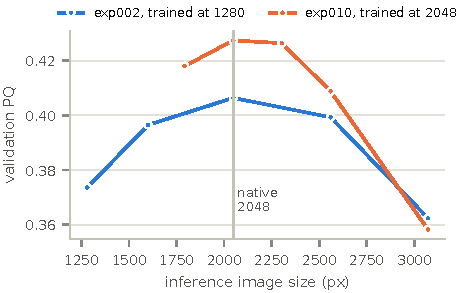
\includegraphics[width=0.66\textwidth]{figures/fig_resolution.pdf}
\caption{Validation PQ against the inference resolution, for a model trained at 1280 pixels (exp002)
and one trained at 2048 (exp010). Both peak at the native frame.
\generatedby{book/make\_book\_figures.py:fig\_resolution}}
\label{fig:yolo-resolution}
\end{figure}

Beyond the native size the score falls. At 3072 pixels SQ is essentially unchanged (0.6728, against
0.6695 at 2048), but RQ drops from 0.607 to 0.539: the masks that are found are no better, and fewer
of them are found. Enlarging an image adds no information that the camera did not record, and it
pushes the objects beyond the range of sizes that the detector learned.

Our first explanation of the peak was that a detector responds best to inputs about 1.6 times larger
than its training size, and $1.6\times1280=2048$. We tested this in exp024, using a model (exp010)
that had been trained at 2048 pixels, for which the explanation predicted a peak near 3300. The peak
was again at 2048. The simpler reading was the correct one: the peak occurs at the \emph{native
frame}, where every recorded pixel is present, and the factor of 1.6 was a coincidence.

\section{Masks that are too wide}\label{sec:yolo-erosion}
Our next experiment, exp005, was built on a hypothesis about thin structures. YOLO thresholds a
smooth mixture of prototypes at one half, so the edges of a thin ridge should be the first parts to
fall below the threshold. The masks should therefore be too \emph{thin}, and growing them by a pixel
should help. The measurement showed the opposite, consistently across the whole range of changes
(Figure~\ref{fig:yolo-erosion}).

\begin{figure}[t]
\centering
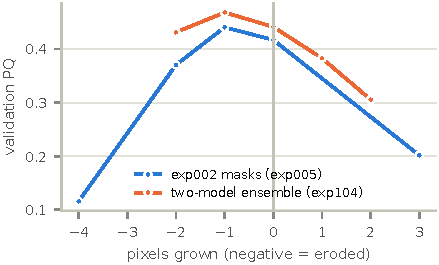
\includegraphics[width=0.66\textwidth]{figures/fig_erosion.pdf}
\caption{Validation PQ after a uniform change to every predicted mask, in pixels. Negative values
erode and positive values dilate. For the masks of exp002, and for the later two-model ensemble, one
pixel of erosion is best. \generatedby{book/make\_book\_figures.py:fig\_erosion}}
\label{fig:yolo-erosion}
\end{figure}

\begin{center}\small
\begin{tabular}{@{}cccccc@{}}
\toprule
pixels grown & PQ (confidence 0.35) & SQ & TP & FP \\
\midrule
$-4$ & 0.1156 & 0.595 & 200 & 535 \\
$-2$ & 0.3702 & 0.651 & 708 & 456 \\
$\mathbf{-1}$ & \textbf{0.4404} & \textbf{0.684} & 845 & 456 \\
$0$ & 0.4169 & 0.671 & 829 & 514 \\
$+3$ & 0.2016 & 0.602 & 448 & 905 \\
\bottomrule
\end{tabular}
\end{center}
Eroding every mask by one pixel, together with a confidence floor raised to 0.35, took the validation
score from 0.4064 to 0.4404 and the public score from 0.33 to 0.36. The optimum lies in the interior
of the grid in both directions: confidence thresholds of 0.30 and 0.40 are both worse, and so are
erosions of 0 and 2 pixels. The optimum is therefore not an artefact of where the grid
happened to end.

Two mechanisms were mixed together in this result. Erosion tightens masks that already match, but it
also shrinks marginal blobs below the minimum area of 300 pixels, so that they are dropped before
they can count as false positives. Repeating the sweep without the area filter separated the two.
The gain was $+0.0235$ with the filter and $+0.0223$ without it, so 95\% of it comes from correcting
the boundaries. SQ confirms this. It is the mean IoU over \emph{matched} pairs, so discarding
unmatched predictions cannot change it, and yet it rose from 0.6707 to 0.6837. Without the area
filter, erosion improved every count at once: true positives rose from 833 to 861, false positives
fell from 533 to 505, and false negatives fell from 492 to 464. This is the signature of a real
improvement to the boundaries. Near misses cross the IoU threshold of one half, and each crossing
turns one false positive and one false negative into one true positive
(Section~\ref{sec:metric-leverage}).

\subsection{Where the extra width came from}\label{sec:yolo-fat-cause}
Section~\ref{sec:masks-fat} traced the cause. Ultralytics draws its training targets with
\texttt{cv2.fillPoly}, whereas the competition scores with \texttt{pycocotools}. On filaments, which
consist mostly of boundary, the two conventions differ by about 11\% of the area. The model learns
the wider convention faithfully and reproduces it at test time.

One pixel of erosion over-corrects: it moves the area of the masks from about 11\% too large to
about 10\% too small. The two conventions differ by about half a pixel, and no operation on a binary
raster can remove half a pixel, because the distance transform of a binary mask takes only whole
steps. The proper fix works in coordinate space: shrink each polygon by 0.5 pixels before it is
rasterised (Listing~\ref{lst:masks-shrink}). This raised the agreement between the training targets
and the scorer's masks from an IoU of 0.898 to 0.959, and moved the ratio of their areas from 1.111
to 0.986. Every YOLO model that we trained afterwards used these corrected targets, and each of them
then performed best with \emph{no} erosion at test time, as one would expect if the targets were
right.

\subsection{Why the correction needs a full-resolution loss}\label{sec:yolo-maskratio}
The correction had a complication, caused by a setting of the library. Ultralytics builds its target
masks at the input size divided by a parameter called \texttt{mask\_ratio}, whose default value is 4,
and it computes the mask loss at that reduced size. At an input of 2048 pixels, the loss grid is
therefore only 512 cells wide, and a correction of half a pixel at 2048 amounts to an eighth of a
cell on the grid that the loss can see (Figure~\ref{fig:yolo-grid}). The correction almost vanishes
before the model is trained on it. The same is true of the error that the correction targets: 64\%
of the disagreement between predicted and annotated masks lies within two native pixels of the
boundary, which is half a cell at 512.

\begin{figure}[t]
\centering
\begin{tikzpicture}[scale=1.0]
  % (a) fine grid: loss at native resolution
  \begin{scope}
    \foreach \cx/\cy in {0/2, 1/2, 4/3, 7/4}
      \fill[vizorange!55] (\cx*0.25,\cy*0.25) rectangle ++(0.25,0.25);
    \draw[gridline, line width=0.4pt] (0,0) grid[step=0.25] (2,2);
    \draw[inkmuted, line width=0.6pt] (0,0) rectangle (2,2);
    \draw[vizblue, line width=1.1pt] (0,0.6) -- (2,1.2);
    \draw[vizblue, line width=1.1pt, dashed] (0,0.47) -- (2,1.07);
    \node[note] at (1,-0.35) {(a) loss on the native grid:\\ the offset flips four pixels};
  \end{scope}
  % (b) coarse grid: loss at a quarter of the resolution
  \begin{scope}[xshift=3.4cm]
    \draw[gridline, line width=0.4pt] (0,0) grid[step=1] (2,2);
    \draw[inkmuted, line width=0.6pt] (0,0) rectangle (2,2);
    \foreach \cx/\cy in {0.5/0.5, 1.5/0.5, 0.5/1.5, 1.5/1.5}
      \fill[inkmuted] (\cx,\cy) circle (1.2pt);
    \draw[vizblue, line width=1.1pt] (0,0.6) -- (2,1.2);
    \draw[vizblue, line width=1.1pt, dashed] (0,0.47) -- (2,1.07);
    \node[note] at (1,-0.35) {(b) loss on a 4$\times$ coarser grid:\\ no pixel centre moves side};
  \end{scope}
  \draw[vizblue, line width=1.1pt] (6.4,1.8) -- (6.9,1.8);
  \node[note, anchor=west] at (6.95,1.8) {annotated edge};
  \draw[vizblue, line width=1.1pt, dashed] (6.4,1.2) -- (6.9,1.2);
  \node[note, anchor=west] at (6.95,1.2) {edge moved inward by\\ half a native pixel};
  \fill[vizorange!55] (6.525,0.43) rectangle ++(0.25,0.25);
  \node[note, anchor=west] at (6.95,0.55) {pixel whose label\\ changes};
\end{tikzpicture}
\caption{Why a correction of half a pixel needs supervision at full resolution. On the native grid
(a), moving an edge inward by half a pixel changes the label of about one pixel in two along the
edge. On a grid four times coarser (b), the same move changes the side of almost no cell centre, so
the loss cannot see it. \drawnin{book/chapters/ch07\_yolo.tex}}
\label{fig:yolo-grid}
\end{figure}

Setting \texttt{mask\_ratio=1} makes the loss grid native. Besides its memory cost, this has a
subtler cost: a larger share of each mask's pixels lies in its interior, so the boundary receives
relatively less weight in the loss. For example, a filament of 1,275 pixels with a perimeter of 200
pixels has 15.7\% of its pixels on its rim at 2048, against about 62\% of its cells at 512. The trade
is nevertheless worth making, because the alternative is a loss that cannot represent the boundary
error at all.

\section{Retraining at native resolution}\label{sec:yolo-retrain}
Everything so far pointed to a single experiment: train at 2048 pixels, with the corrected targets
and \texttt{mask\_ratio=1}, until the training schedule has run to completion. Running that experiment
properly took five attempts and most of a week. We describe the attempts in turn, because each one
failed for a different reason, and several of the reasons recur in later chapters.

\subsection{exp010: two of three changes silently lost}\label{sec:yolo-exp010}
Experiment exp010 trained at 2048 pixels on a T4 GPU for Kaggle's twelve-hour limit. When we read
its configuration file afterwards, it said \texttt{mask\_ratio: 2}. The training script contained a
fallback ladder for memory errors, and when full-resolution supervision ran out of memory at batch
sizes 2 and 1, the script quietly moved to the third rung. At \texttt{mask\_ratio=2}, the half-pixel
correction is a quarter of a cell on the loss grid, so the corrected targets were again nearly
ineffective. In addition, the cosine learning-rate schedule~\citep{sgdr} had been sized for 400 epochs, and the
session reached only epoch 62. After twelve hours the learning rate was still 94\% of its peak value
of $10^{-3}$, so the model never went through the phase of low learning rates in which fine-tuning
earns much of its final accuracy. It scored 0.4274 on validation and 0.36 on the leaderboard.

\subsection{exp031: a completed schedule at 1536 pixels}\label{sec:yolo-exp031}
Experiment exp031 fixed both faults at the cost of some resolution: it trained at 1536 pixels, with
batch size 1, \texttt{mask\_ratio=1}, a frozen backbone, and 50 epochs of a cosine schedule that
annealed from $5\times10^{-4}$ to $5.5\times10^{-6}$. Getting it to run took five launches and two
wrong diagnoses. Freezing the backbone did not free the memory that we had expected it to free,
because the allocation that failed was a single tensor in the mask loss, whose size grows with the
number of filaments in the batch. This also explained why a single crowded photograph could end a
run five epochs after it started. A second problem was that several attempts made inside one
Python process produced byte-identical out-of-memory errors, because \texttt{torch.cuda.empty\_cache()} cannot
release memory that the previous trainer still references; running each attempt in a separate
process solved this. The run scored 0.4343 on validation and 0.36 on the leaderboard.

At this point four of our models, exp002, exp010, exp031 and a fusion of the first two, all appeared
on the leaderboard as 0.36. Their validation scores ranged from 0.4274 to 0.4411, a spread of 0.0137,
which is smaller than one step of the two-decimal leaderboard. Section~\ref{sec:val-transfer}
explains why differences of this size cannot be seen on the leaderboard, and why we needed a
different kind of change.

\subsection{exp067--exp073: native supervision that fits in memory}\label{sec:yolo-memory}
Why does the mask loss need so much memory? The answer is that every positive \emph{location}, not
every filament, expands a full-size target map and a full-size map of logits, and each filament has
up to ten positive locations (Section~\ref{sec:yolo-training}). The chunked mask loss in
\file{shared/chunked\_mask\_loss.py} processes the positive locations in small groups, and recomputes
each group during the backward pass instead of storing its intermediate results, a technique known as
\keyterm{activation checkpointing}~\citep{checkpointing}. This made \texttt{mask\_ratio=1} at 2048 pixels fit on a T4.

Its first run produced losses of NaN in 16-bit arithmetic, and the cause is worth recording. To keep
every parameter connected to the computational graph, the loss added the term
\texttt{proto.sum() * 0}. A sum over a large half-precision tensor can overflow to infinity, and
$\infty\times0$ is NaN. Connecting the parameters through a single element of the tensor, instead of
through its sum, fixed the problem, and we moved validation to 32-bit arithmetic. The model of exp068
then trained for five epochs (2.5 hours) and scored 0.4470 with test-time augmentation, below the
0.4586 of our best pipeline at that time.

The ROI loss in \file{shared/roi\_mask\_loss.py} made the same supervision nearly twice as fast,
using a simple observation from linear algebra. Upsampling is a linear operation, so for any
upsampling operator $U$ we have
\begin{equation}
U\Big(\sum_{j} c_{dj} P_j\Big) = \sum_{j} c_{dj}\, U(P_j).
\end{equation}
The standard loss first upsamples all 32 prototypes to the native size and then mixes them. The ROI
loss mixes them first, at a quarter of the resolution, which leaves a single map, and then samples
that map at the native resolution only inside the detection's box, using the differentiable
bilinear sampling of spatial transformer networks~\citep{jaderberg2015}
(Listing~\ref{lst:yolo-roi}). The
result is the same up to floating-point rounding, and the cost falls from 32 native-size maps per
image to one small map per detection.

\begin{lstlisting}[caption={A native-resolution mask loss evaluated only inside the box. Condensed
from \file{shared/roi\_mask\_loss.py}.},label=lst:yolo-roi]
def roi_mask_loss(coefficient, proto, truth, box, area, height, width):
    x0, y0, x1, y1 = box                                   # integer box at native resolution
    # mix FIRST: one low-resolution logit map instead of 32 upsampled prototypes
    low = (coefficient.float() @ proto.float().flatten(1)).reshape(1, 1, *proto.shape[-2:])
    # centres of the native pixels inside the box, in grid_sample's [-1, 1] coordinates
    x = (torch.arange(x0, x1, dtype=torch.float32) + 0.5) * (2 / width) - 1
    y = (torch.arange(y0, y1, dtype=torch.float32) + 0.5) * (2 / height) - 1
    yy, xx = torch.meshgrid(y, x, indexing="ij")
    grid = torch.stack([xx, yy], dim=-1)[None]
    logits = F.grid_sample(low, grid, mode="bilinear", padding_mode="border",
                           align_corners=False)[0, 0]    # same as upsample-then-crop
    return F.binary_cross_entropy_with_logits(logits, truth[y0:y1, x0:x1].float(),
                                              reduction="sum") / (height * width * area)
\end{lstlisting}

On the same crowded photographs, a full optimiser step took 1.58 seconds with the ROI loss and 2.86
seconds with the chunked loss, and peak memory fell from 9.4 to 5.9 GiB. Experiment exp073 continued
the training of exp068 with the ROI loss for four more epochs and reached 0.4555, still below 0.4586.

\subsection{exp097: a converged YOLOv8l-seg at 2048 pixels}\label{sec:yolo-exp097}
Our last YOLO run rented a 48 GB L40 GPU on RunPod at \$0.69 an hour, and trained the larger
YOLOv8l-seg at 2048 pixels, with the corrected targets, a batch size of 2, and full-resolution
supervision. Three engineering decisions defined the run.
\begin{enumerate}[leftmargin=*,itemsep=2pt]
\item \textbf{Its length was decided by convergence.} After the warm-up, the
learning rate stayed constant. When a three-epoch moving average of the validation fitness had not
improved by 0.002 for 12 epochs, the learning rate was multiplied by 0.2. After three such
reductions, a further plateau stopped the training (Algorithm~\ref{alg:yolo-plateau} and
Listing~\ref{lst:yolo-plateau}).
\item \textbf{Its batch size was measured.} A preflight step trained for a few iterations on the most
crowded images at each candidate batch size and chose the fastest one that fitted in memory. This was
a batch size of 2, which processed 9.4 images per second and used 39,396 of the GPU's 45,458 MiB.
\item \textbf{It was rehearsed on free hardware.} The second rented machine failed 35 seconds after
training began, because of a defect in our own callbacks. They had been written against an assumed
version of the Ultralytics API and tested only against that assumption. Reading the source code of
the pinned version of the library revealed four defects. After that, every payload was first run on
a free Kaggle T4 (exp099, with 23 automated checks) before any money was spent.
\end{enumerate}

\begin{algorithmblock}{Learning-rate decay on plateau, with stopping at convergence\label{alg:yolo-plateau}}
\item \textbf{parameters:} patience $n_p=12$ epochs, minimum improvement $\delta=0.002$, decay factor $0.2$, at most 3 decays
\item \textbf{after each epoch} (once the warm-up is over and three fitness values exist) \textbf{do}
\item \Ind $\bar f\leftarrow$ mean fitness of the last three epochs;
\item \Ind \textbf{if} $\bar f>f^{\ast}+\delta$ \textbf{then} $f^{\ast}\leftarrow\bar f$; reset the plateau counter; \textbf{continue};
\item \Ind increment the plateau counter; \textbf{if} it is below $n_p$ \textbf{then} \textbf{continue};
\item \Ind \textbf{if} fewer than 3 decays so far \textbf{then} multiply the learning rate by 0.2 and reset the counter;
\item \Ind \textbf{else} stop training: the model has converged at every learning rate tried
\end{algorithmblock}

\begin{lstlisting}[caption={Decay on plateau, stop at convergence. Condensed from
\file{experiments/exp\_097\_runpod\_yolo/src/convergence.py}.},label=lst:yolo-plateau]
def update(self, epoch, fitness):          # patience 12, min_delta 0.002, decay 0.2, 3 decays
    self.window.append(fitness)             # deque(maxlen=3): a moving average
    smoothed = sum(self.window) / len(self.window) if len(self.window) == 3 else None
    if epoch <= self.warmup_epochs or smoothed is None:
        return "continue"
    if self.best is None or smoothed > self.best + self.min_delta:
        self.best, self.best_epoch, self.since_best = smoothed, epoch, 0
        return "continue"                   # improved
    self.since_best += 1
    if self.since_best < self.patience:
        return "continue"                   # plateau, still counting
    if self.decays < self.max_decays:
        self.decays += 1; self.lr_scale *= self.decay_factor; self.since_best = 0
        return "decay"                      # every lower rate gets a full window
    return "stop"                           # converged at every rate tried
\end{lstlisting}

The run behaved as designed. The first stage reached a plateau and was decayed at epoch 75, and the
first decay lifted the fitness from 0.648 to 0.686 within six epochs. Training stopped at epoch 124
after three decays, having used learning rates of $10^{-3}$, $2\times10^{-4}$, $4\times10^{-5}$ and
$8\times10^{-6}$. The best fitness occurred at epochs 86 to 88, and the final mask mAP50 was 0.704.
The run cost \$2.74.

Scored with our own pipeline, the best checkpoint reached 0.4668 with test-time augmentation, which
made it the best YOLO model we produced. It appeared on the leaderboard as 0.39. Two further findings
came with it. First, the checkpoints saved at the second and third decays contained exactly the same
weights as the best checkpoint, because nothing after epoch 88 improved the fitness; the last 36
epochs bought nothing. Second, the checkpoint from the end of the first stage, whose fitness was
only 0.047 lower, scored just 0.4538. Fitness measures ranking, whereas PQ measures a single emitted
set, and the relationship between the two is not constant.

\section{What the YOLO models could and could not do}\label{sec:yolo-lessons}
The YOLO models took the public score from 0.32 to 0.39, through inference at the native resolution,
corrected targets, test-time augmentation (Chapter~\ref{ch:tta}) and ensembles. A converged model,
trained at the native resolution with correct targets and full-resolution supervision, still
appeared as 0.39, and we did not find a way to take this family further.

A public notebook from a team with a leaderboard score of about 0.55 runs YOLOv8l-seg at 2048 pixels
with a confidence floor of 0.30. It contains a defect: it orders overlapping masks by their class
index, which is zero for every mask, instead of by their confidence. In exp095 we ran the notebook's
inference procedure on our own weights from exp002 (YOLO11m-seg trained at 1280 pixels). It scored
0.4111, against 0.4469 for our best single-view procedure on the same weights. If that team's
advantage is real, it must therefore lie in its trained model rather than in its inference
procedure. Our own
YOLOv8l-seg, trained at the same resolution to convergence, appeared as 0.39, and we never explained
the gap.

Ultralytics also taught us to distrust configuration. The library changes what one asks for without
failing, and each of the following behaviours affected one of our runs.
\begin{itemize}[leftmargin=*,itemsep=1pt]
\item With \texttt{optimizer="auto"}, the library ignores \texttt{lr0} and chooses its own optimiser
and learning rate.
\item A bare \texttt{resume=True} searches the library's own settings folder for a run to resume,
and ignores the folder of the current project.
\item Removing the \texttt{time=} argument also removes the rescaling of the learning-rate schedule
to the time budget.
\item Setting \texttt{augment=True} on a segmentation model logs a warning and runs at a single
scale.
\item An out-of-memory error in the first epoch halves the batch size and rebuilds the optimiser.
\end{itemize}
The defence is to read back the resolved configuration of every run (the file \file{args.yaml}),
and to check the learning rate that the optimiser actually uses rather than the one that was
passed to it.

Finally, the question raised in Section~\ref{sec:yolo-prototypes}, whether the 32-prototype basis
limits the masks, was never settled cleanly. The most direct test, a converged model at the native
resolution, gained 0.011 on validation over our standing baseline. This was neither the collapse nor
the leap that would have answered the question. What the YOLO experiments did establish is that no
further gain of the size we needed was available from this family of models, and this led us to a
model that predicts each mask from its own query (Chapter~\ref{ch:transformers}).

\section*{Exercises}
\begin{exercise}{The size of the basis}
A mask in Equation~\eqref{eq:yolo-mask} is a thresholded combination of 32 maps at a quarter of the
resolution. Take one annotated filament, downsample its mask by a factor of 4, and fit the best
combination of 32 smooth random maps to it (least squares on the logits). How does the IoU of the
reconstruction depend on the width of the filament? Compare a thin filament with a thick one.
\end{exercise}

\begin{exercise}{Why the threshold sweep is flat}
Using the first and last rows of the threshold table in Section~\ref{sec:yolo-exp002}, compute the
change in the numerator and in the denominator of PQ between the confidence thresholds 0.30 and
0.20. Explain why 59 extra true positives bought nothing.
\end{exercise}

\begin{exercise}{Counting flipped pixels}
In Figure~\ref{fig:yolo-grid}, an edge moves inward by half a native pixel. Show that on a grid whose
cells are $s$ native pixels wide, the expected fraction of cells along the edge whose centres change
side is $\min(1, 0.5/s)$. Evaluate this fraction for \texttt{mask\_ratio} values of 1, 2 and 4 at an
input size of 2048.
\end{exercise}

\begin{exercise}{Linearity of upsampling}
Prove that bilinear interpolation is a linear operator. Then verify numerically that
Listing~\ref{lst:yolo-roi} gives the same logits as upsampling all 32 prototypes with
\texttt{F.interpolate(..., mode="bilinear", align\_corners=False)} and then cropping.
\end{exercise}

\begin{exercise}{A controller on a noisy curve}
Simulate fitness curves as a saturating function of the epoch plus Gaussian noise with a standard
deviation of 0.01. Run Algorithm~\ref{alg:yolo-plateau} on them, and measure how often it decays too
early as the length of the moving-average window changes from 1 to 5.
\end{exercise}

\chapter{Test-Time Augmentation and Ensembles}\label{ch:tta}

\section{Introduction}\label{sec:tta-why}
Averaging several noisy predictions is one of the oldest ideas in machine
learning~\citep{dietterich2000}. Suppose that each of $n$ predictions of some quantity has an error
with variance $\sigma^2$, and that every pair of errors has correlation $\rho$. The variance of
their average is then~\citep{hastie2009}
\begin{equation}
\operatorname{Var}\Big(\frac1n\sum_{v=1}^{n}\hat y_v\Big)
= \frac{\sigma^2}{n} + \frac{n-1}{n}\,\rho\,\sigma^2
= \sigma^2\Big(\rho + \frac{1-\rho}{n}\Big).
\label{eq:tta-variance}
\end{equation}
If the errors are independent ($\rho=0$), eight predictions reduce the variance eightfold. If they
are correlated, the variance of the average can never fall below $\rho\sigma^2$, however many
predictions we average. For example, with $\rho=0.9$, eight predictions remove less than a tenth of
the variance.

Equation~\eqref{eq:tta-variance} summarises most of this chapter. We tried two ways of obtaining
several predictions for the same photograph. \keyterm{Test-time augmentation}
(TTA)~\citep{krizhevsky2012} feeds a single model several transformed copies of the photograph, and
an \keyterm{ensemble}~\citep{lakshminarayanan2017} feeds the photograph to several models. Both help only to the extent that the errors of the individual predictions are
independent, and in our problem the errors turned out to be largely shared. In
Section~\ref{sec:tta-d4} we describe the transformations we used, and in Section~\ref{sec:tta-fusion}
the algorithm that combines instance masks from several views. Section~\ref{sec:tta-ensembles}
describes our ensembles of models, and Section~\ref{sec:tta-calibration} shows how to make the
confidence scores of different models comparable before combining them.
Section~\ref{sec:tta-m2f} applies test-time augmentation to the final model, and
Section~\ref{sec:tta-lesson} discusses what all these results say about the errors.

\section{The dihedral group}\label{sec:tta-d4}
The photographs have no preferred left or right, and a rotated image of the disk is still a
plausible image of the disk. Many astronomical images share this property, and \citet{dieleman2015}
exploited it in a network that classifies galaxies. The natural transformations are therefore the eight symmetries of a
square, which form the \keyterm{dihedral group} $D_4$: the four rotations by multiples of
$90^\circ$, each with or without a mirror reflection,
\begin{equation}
D_4 = \{\, r^k,\; f r^k \;:\; k = 0,1,2,3 \,\},
\end{equation}
where $r$ rotates the image by $90^\circ$ and $f$ reflects it from left to right. These
transformations move pixels without interpolating them, so no information is lost or invented,
unlike the rescaling of Section~\ref{sec:yolo-resolution}. Figure~\ref{fig:tta-d4} shows them
applied to a real filament.

\begin{figure}[t]
\centering
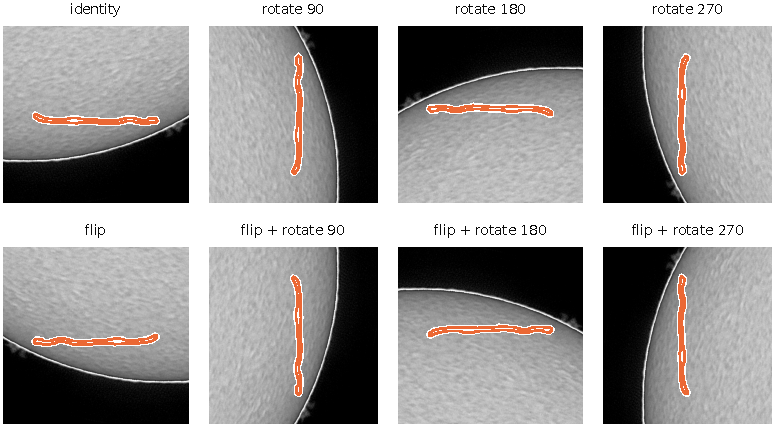
\includegraphics[width=\textwidth]{figures/fig_d4.pdf}
\caption{The eight dihedral views of one annotated filament, whose outline is drawn in orange. Each
view is a legitimate photograph of the same object, and a model sees each one slightly differently.
\generatedby{book/make\_book\_figures.py:fig\_d4}}
\label{fig:tta-d4}
\end{figure}

Test-time augmentation with $D_4$ runs the model once on each view and maps each predicted mask back
to the original orientation with the inverse transformation:
\begin{equation}
\mathcal{M}_g = \big\{\, g^{-1}(m) \;:\; m \in \mathrm{model}(g(\mathbf{x})) \,\big\},
\qquad g \in D_4 .
\end{equation}
If the model were exactly \keyterm{equivariant} to these transformations, meaning that
$\mathrm{model}(g(\mathbf{x})) = g(\mathrm{model}(\mathbf{x}))$ for every $g$, then all eight sets
$\mathcal{M}_g$ would be identical and TTA would change nothing. Convolutional networks are
equivariant to translations by construction, but not to rotations or reflections. Networks that
are equivariant to these transformations by construction exist~\citep{cohen2016}, but we did not use
one. Training with
flipped and rotated copies of the images makes them only approximately equivariant, and TTA exploits
the part of the equivariance that training did not achieve.

We also tried transformations of intensity. Applying a gamma curve to the photograph gave a PQ of
0.4294 at $\gamma=0.8$ and 0.4347 at $\gamma=1.2$, both below the 0.4411 obtained from the unchanged
image, so we dropped them.

\section{Fusing instances across views}\label{sec:tta-fusion}
For a semantic model, test-time augmentation is easy: we simply average the eight probability maps
pixel by pixel, as we did in exp004. For an instance model it requires a real algorithm, because
nothing tells us which mask in one view corresponds to which mask in another. One view may split a
filament that another view keeps whole, and each view has its own set of low-confidence extras. The
fusion rule in \file{experiments/exp\_033\_inference/src/cached\_tta.py} handles this greedily, in
the spirit of the weighted boxes fusion that detectors use~\citep{solovyev2021}, as described in
Algorithm~\ref{alg:tta-fuse} and Figure~\ref{fig:tta-fusion}.

\begin{algorithmblock}{Greedy fusion of instance masks across $N$ views\label{alg:tta-fuse}}
\item \textbf{input:} the scored masks of all $N$ views, mapped back to the original orientation; link threshold $\lambda=0.5$; vote fraction $\nu=0.5$
\item pool the masks of all views and sort them by decreasing score;
\item \textbf{while} some mask is unused \textbf{do}
\item \Ind take the most confident unused mask as the \emph{seed} of a new cluster;
\item \Ind add to the cluster every unused mask whose IoU with the seed is at least $\lambda$, and mark all members used;
\item \Ind fused mask $\leftarrow$ the pixels contained in at least $\max(1,\operatorname{round}(\nu n))$ of the cluster's $n$ members;
\item \Ind fused score $\leftarrow$ (mean score of the members) $\times\,\bigl(\tfrac12+\tfrac12\,n/N\bigr)$;
\item \Ind keep the fused mask if its area is at least 40 pixels;
\item \textbf{return} the fused masks and their scores
\end{algorithmblock}

The last factor in the fused score rewards \keyterm{support}, the share of the views that found the
object. A filament that all eight views found keeps its mean confidence, whereas a filament that
only one view found loses almost half of it.

\begin{figure}[t]
\centering
\begin{tikzpicture}[
  st/.style={box=#1, text width=1.95cm, minimum height=1.25cm, font=\sffamily\scriptsize,
             execute at begin node={\hyphenpenalty=10000}}]
  \node[st=inkmuted] (a) at (0,0) {predict on 8 views; map each mask back};
  \node[st=vizblue] (b) at (2.6,0) {pool all masks; sort by confidence};
  \node[st=vizblue] (c) at (5.2,0) {seed: best unused mask; members: IoU with seed $\ge 0.5$};
  \node[st=vizaqua] (d) at (7.8,0) {pixel vote: keep pixels in $\ge$ half of the members};
  \node[st=vizorange] (e) at (10.4,0) {score $=$ mean $\times\,(\frac12+\frac12\,n/N)$};
  \draw[flow] (a) -- (b); \draw[flow] (b) -- (c); \draw[flow] (c) -- (d); \draw[flow] (d) -- (e);
  \draw[flow] (e.south) -- ++(0,-0.45) -| node[note, pos=0.25, below=1pt] {repeat until every mask is used} (c.south);
\end{tikzpicture}
\caption{Instance fusion across test-time views. Clusters are seeded greedily in order of
confidence; each cluster's mask is a pixel vote among its members, and its score rewards support from
many views. \drawnin{book/chapters/ch08\_tta.tex}}
\label{fig:tta-fusion}
\end{figure}

The pixel vote in Algorithm~\ref{alg:tta-fuse} also controls the width of the fused mask.
Figure~\ref{fig:tta-vote} shows how the vote fraction affects a cluster of three overlapping member
masks. Requiring a vote from one member gives the union, which
grows the mask; requiring all members gives the intersection, which shrinks it; the majority vote
lies between the two. Recall from Section~\ref{sec:yolo-erosion} that the early YOLO masks were
already slightly too wide. The vote fraction therefore also acts as a control on the boundary, and a
later experiment (exp132) found that a stricter vote could replace the one-pixel erosion.

\begin{figure}[t]
\centering
\begin{tikzpicture}
  \foreach \px/\lab in {0/{at least 1 of 3: union}, 3.6/{at least 2 of 3: majority}, 7.2/{3 of 3: intersection}}{
    \node[note] at (\px,-0.85) {\lab};
  }
  % union
  \begin{scope}
    \fill[vizblue!45, rotate around={12:(0,0)}] (0,0) ellipse (1.0 and 0.33);
    \fill[vizblue!45, rotate around={4:(0.18,0.07)}] (0.18,0.07) ellipse (0.95 and 0.3);
    \fill[vizblue!45, rotate around={20:(-0.12,-0.04)}] (-0.12,-0.04) ellipse (1.05 and 0.28);
  \end{scope}
  % majority: union of the three pairwise intersections
  \begin{scope}[xshift=3.6cm]
    \begin{scope}
      \clip[rotate around={12:(0,0)}] (0,0) ellipse (1.0 and 0.33);
      \fill[vizblue!45, rotate around={4:(0.18,0.07)}] (0.18,0.07) ellipse (0.95 and 0.3);
      \fill[vizblue!45, rotate around={20:(-0.12,-0.04)}] (-0.12,-0.04) ellipse (1.05 and 0.28);
    \end{scope}
    \begin{scope}
      \clip[rotate around={4:(0.18,0.07)}] (0.18,0.07) ellipse (0.95 and 0.3);
      \fill[vizblue!45, rotate around={20:(-0.12,-0.04)}] (-0.12,-0.04) ellipse (1.05 and 0.28);
    \end{scope}
  \end{scope}
  % intersection
  \begin{scope}[xshift=7.2cm]
    \begin{scope}
      \clip[rotate around={12:(0,0)}] (0,0) ellipse (1.0 and 0.33);
      \clip[rotate around={4:(0.18,0.07)}] (0.18,0.07) ellipse (0.95 and 0.3);
      \fill[vizblue!45, rotate around={20:(-0.12,-0.04)}] (-0.12,-0.04) ellipse (1.05 and 0.28);
    \end{scope}
  \end{scope}
  % outlines of the three members in every panel
  \foreach \px in {0, 3.6, 7.2}{
    \begin{scope}[xshift=\px cm]
      \draw[vizorange, line width=0.6pt, rotate around={12:(0,0)}] (0,0) ellipse (1.0 and 0.33);
      \draw[vizaqua!80!black, line width=0.6pt, rotate around={4:(0.18,0.07)}] (0.18,0.07) ellipse (0.95 and 0.3);
      \draw[vizviolet, line width=0.6pt, rotate around={20:(-0.12,-0.04)}] (-0.12,-0.04) ellipse (1.05 and 0.28);
    \end{scope}
  }
\end{tikzpicture}
\caption{The pixel vote inside one cluster of three member masks, whose outlines are drawn in
colour. The region that is kept (blue) shrinks as the required share of members rises.
\drawnin{book/chapters/ch08\_tta.tex}}
\label{fig:tta-vote}
\end{figure}

\subsection{Voting on run-length encodings *}\label{sec:tta-ladder}
Our implementation performs the vote on run-length encodings, without ever decoding a mask into a
$2048\times2048$ array. It maintains a ladder of running regions, in which level $k$ holds the
pixels covered by at least $k$ of the masks seen so far. Each new mask $M$ updates the ladder from the
top down: level $k$ gains the pixels of level $k-1$ that $M$ also covers, and level 1 gains $M$
itself. After the last mask has been processed, the level equal to the required number of votes is
the answer. Listing~\ref{lst:tta-fuse} shows the ladder and the fusion loop.

\begin{lstlisting}[caption={Exact $k$-of-$n$ voting on RLE, and the greedy fusion. Condensed from
\file{experiments/exp\_033\_inference/src/cached\_tta.py} and
\file{experiments/exp\_097\_runpod\_yolo/src/evaluate\_ensemble.py}.},label=lst:tta-fuse]
def vote_rle(masks, needed):
    levels = [None] * needed          # levels[k-1]: pixels covered by >= k masks so far
    for i, mask in enumerate(masks):
        for k in range(min(i + 1, needed), 1, -1):          # top of the ladder first
            both = mu.merge([levels[k - 2], mask], intersect=True)
            levels[k - 1] = both if levels[k - 1] is None else mu.merge([levels[k - 1], both])
        levels[0] = mask if levels[0] is None else mu.merge([levels[0], mask])
    return levels[-1]

def fuse(entries, link=0.5, vote=0.5, sources=8):    # entries: (score, rle) from every view
    order = sorted(range(len(entries)), key=lambda i: -entries[i][0])
    rles = [e[1] for e in entries]
    ious = mu.iou(rles, rles, [0] * len(rles))          # pycocotools works on RLE directly
    used, output = set(), []
    for seed in order:
        if seed in used:
            continue
        used.add(seed)
        members = [seed] + [i for i in order if i not in used and ious[seed, i] >= link]
        used.update(members)
        binary = vote_rle([rles[i] for i in members], max(1, round(vote * len(members))))
        if mu.area(binary) < 40:
            continue
        score = float(np.mean([entries[i][0] for i in members]))
        output.append(dict(score=score * (0.5 + 0.5 * len(members) / sources), rle=binary))
    return output
\end{lstlisting}

\subsection{Example: the first attempt lost}\label{sec:tta-first}
Our first TTA experiment (exp007) used the same idea and \emph{lost}: the best of twelve fusion
settings scored 0.4035, against 0.4404 for a single view. At the time we identified two plausible
mechanisms, errors in the clustering and a vote that further eroded masks that had already been
trimmed, and we concluded that the result was a verdict on that particular implementation rather
than on TTA in general.

When we returned to the idea, we found a step that the first evaluation had skipped: it never
re-swept the confidence threshold after fusion. The support factor in Algorithm~\ref{alg:tta-fuse}
changes the scale of the scores. A filament found by every view keeps its mean confidence, whereas
one found by a single view loses almost half of it, so a threshold tuned for single-view scores is
wrong for fused scores. With the threshold swept again, the same fusion scored 0.4571 on validation.
A bootstrap over photographs (Section~\ref{sec:metric-uncertainty}, with 20,000 resamples) put the
gain at $+0.0166$, with a 95\% interval of $[+0.0039, +0.0303]$ and a probability of 0.995 that the
gain was positive. The fused model appeared on the leaderboard as 0.38, up from 0.36, and with the
emission threshold lowered to 0.35 it appeared as 0.39.

The general point is that any step that changes how scores are computed, such as fusion,
calibration, a support term or a new model, also moves the best operating point, so the confidence
threshold must be swept again after every such step. The grid of thresholds must also extend far
enough. The same problem appeared later, when a sweep started at 0.25 and the best fused rule lay at
the lower edge of the grid; we had to extend the grid down to 0.10.

\subsection{Variants that did not help}\label{sec:tta-variants}
Once the fusion worked, we tested its obvious variations, and none of them improved on it.
\begin{itemize}[leftmargin=*,itemsep=2pt]
\item \textbf{Soft voting.} Averaging the eight mask \emph{probabilities} before thresholding, instead
of voting on binary masks, scored at best 0.4569, against 0.4585 for the corresponding hard vote. It
found the same 841 true positives with six more false positives. Submitted as a probe, it appeared
on the leaderboard as 0.38.
\item \textbf{Mask non-maximum suppression.} Suppressing duplicates by the IoU of their masks rather
than of their boxes helped a single view (0.4453 against 0.4415), but it remained well below fusion,
and it appeared as 0.37.
\item \textbf{Other support scores.} Scoring clusters by the plain mean confidence of their members
(0.4466), or with a linear support term (0.4548), both lost to the rule of
Algorithm~\ref{alg:tta-fuse} (0.4571).
\item \textbf{Pruning by the number of views.} Removing clusters that fewer views supported always
reduced PQ. Most of the clusters that we kept were supported by all eight views, so agreement among
the views does not separate useful masks from harmful ones.
\end{itemize}

\section{Ensembles of models}\label{sec:tta-ensembles}
Fusing the predictions of \emph{different models} uses the same machinery with more sources. We built
ensembles of every kind we could, and Figure~\ref{fig:tta-ensembles} collects the results.

\begin{figure}[t]
\centering
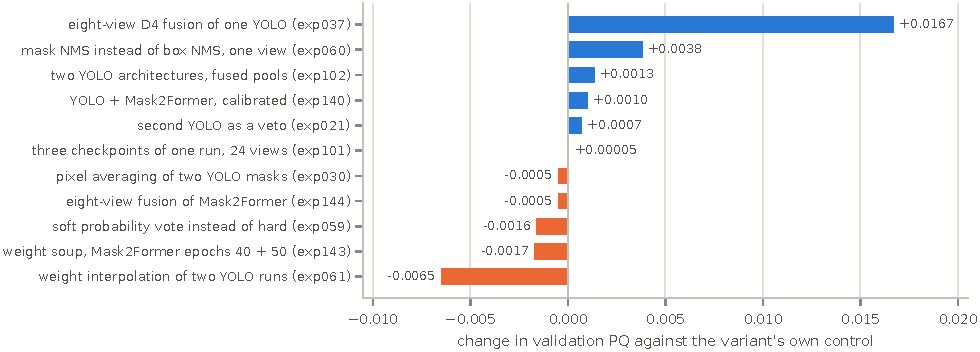
\includegraphics[width=\textwidth]{figures/fig_ensembles.pdf}
\caption{Every fusion, ensemble and weight-averaging variant we measured, shown as the change in
validation PQ relative to that variant's own control. Only the test-time fusion of the first YOLO
model moved the score by more than 0.004.
\generatedby{book/make\_book\_figures.py:fig\_ensembles}}
\label{fig:tta-ensembles}
\end{figure}

\paragraph{Two runs of the same architecture.} The models of exp002 and exp010 err in opposite
directions: the first gains recall at the cost of false positives, and the second gains precision at
the cost of misses. This looks like the textbook situation for an ensemble, but it did not work.
Their union scored 0.4124, requiring both models to agree scored 0.3740, and the best rule, which
used exp010 to veto the weaker masks of exp002, gained 0.0007 by removing 7 of 456 false positives.
The explanation lay in the errors themselves. Most of the false positives of exp002 were filaments
that the annotator of that record had not drawn, and exp010 saw the same filaments and predicted
them too. Averaging the two models' masks pixel by pixel (exp030) also lost. Of the 836 masks, 618
had a partner at an IoU of 0.5 in the other model, and the two models disagreed in the same places.

\paragraph{Checkpoints of one run.} In exp101 we pooled three checkpoints of the converged
YOLOv8l-seg run, with eight views each, for 24 views in all, and gained 0.00005. Checkpoints taken
from one training trajectory share almost all of their mistakes.

\paragraph{Averaging weights instead of predictions.} A \keyterm{model soup}~\citep{soups} averages
the weights of several models fine-tuned from the same starting point, and costs nothing at test
time.\footnote{Averaging weights tends to work when the models lie in the same basin of the loss
surface, as models fine-tuned from the same pretrained weights often do. \citet{soups} showed that
such averages can match or exceed the accuracy of the best individual model, and
\citet{izmailov2018} made a related observation for weights averaged along a single training
run.} Interpolating between exp002 and exp031 lost at every mixing weight (the best was 0.4349,
against 0.4415), and a soup of the Mask2Former's checkpoints from epochs 40 and 50 lost 0.0017 and
appeared on the leaderboard as 0.40, against 0.41 for epoch 40 alone.

\paragraph{Two YOLO architectures.} The first ensemble that helped at all combined models that
differed in more than their random seed: YOLO11m-seg trained at 1280 pixels and YOLOv8l-seg trained
at 2048. Each was first fused over its own eight views, and the two results were then fused with each
other. The ensemble gained 0.0013 and needed its own threshold sweep, because a mixed pool has a
different distribution of scores from either of its parents. As exp119, it appeared on the
leaderboard as 0.39, the same as its best member.

\section{Calibration: making scores comparable}\label{sec:tta-calibration}
Fusion averages the scores of the members of a cluster, which assumes that the scores mean the same
thing. For our models they did not. The best confidence threshold of the Mask2Former was 0.85,
whereas that of the YOLO models was 0.35, so averaging raw scores lets one model's scale dominate.
In exp140 we therefore \keyterm{calibrated}~\citep{guo2017} each source before fusing it, replacing each score by an
estimate of the probability that the metric cares about (Section~\ref{sec:recall-verifiers} explains
why the choice of this probability matters). We defined it as the fraction of a photograph's
annotation records that contain a filament matching the candidate with an IoU above 0.5.

The map from scores to probabilities should be monotone, since a higher score should never mean a
lower probability, but it need not be linear or sigmoidal. \keyterm{Isotonic
regression}~\citep{isotonic} fits exactly such a map. Given scores $s_i$ with labels $y_i$, it finds
the non-decreasing function $f$ that minimises
\begin{equation}
\sum_i \big(y_i - f(s_i)\big)^2 \quad\text{subject to}\quad s_i \le s_j \Rightarrow f(s_i)\le f(s_j).
\end{equation}
The \keyterm{pool-adjacent-violators} algorithm~\citep{ayer1955} solves this problem in a single pass over the sorted
scores (Algorithm~\ref{alg:tta-pav}). Each distinct score starts as its own block. Whenever a block's
mean label is lower than the mean of the block before it, the two blocks violate the monotonicity
constraint, so we merge them, and we keep merging backwards until the block means increase again.
The final block means are the fitted values.

\begin{algorithmblock}{Pool adjacent violators, for isotonic regression\label{alg:tta-pav}}
\item \textbf{input:} the distinct scores in increasing order, each with the sum and count of its labels
\item \textbf{for} each distinct score, in increasing order, \textbf{do}
\item \Ind push a new block containing that score's label sum and count onto a stack;
\item \Ind \textbf{while} the stack has at least two blocks and the mean of the second-last exceeds the mean of the last \textbf{do}
\item \Ind\Ind merge the last two blocks by adding their label sums and counts;
\item \textbf{return} the mean label of each block, as a step function of the score
\end{algorithmblock}

\begin{lstlisting}[caption={Isotonic calibration by pool-adjacent-violators. Condensed from
\file{experiments/exp\_140\_three\_way\_ensemble/src/ensemble.py}.},label=lst:tta-isotonic]
def isotonic_fit(scores, labels):
    values, inverse, counts = np.unique(scores, return_inverse=True, return_counts=True)
    sums = np.bincount(inverse, weights=labels)
    blocks = []                                   # [sum of labels, weight, sum of scores]
    for x, s, c in zip(values, sums, counts):
        blocks.append([s, float(c), x * c])
        while len(blocks) > 1 and blocks[-2][0] / blocks[-2][1] > blocks[-1][0] / blocks[-1][1]:
            s2, c2, sx2 = blocks.pop()            # a violation: pool with the block before
            blocks[-1][0] += s2; blocks[-1][1] += c2; blocks[-1][2] += sx2
    centres = np.array([b[2] / b[1] for b in blocks])
    means = np.array([b[0] / b[1] for b in blocks])
    return centres, means                         # apply with np.interp(score, centres, means)
\end{lstlisting}

We fitted the maps on the validation split. To obtain validation numbers that were not biased by
this fitting, we \keyterm{cross-fitted} them~\citep{chernozhukov2018}: we split the photographs into two folds and calibrated
the candidates of each fold with a map fitted on the other fold, so that no candidate was calibrated
using its own photograph. The fitted maps were informative in themselves. The Mask2Former turned out
to be over-confident in the middle of its range: a score of 0.854 corresponded to a 45\% chance of
matching a record, 0.94 to 64\%, and 0.97 to 88\%. The YOLO models were closer to being calibrated.
The results were as follows:
\begin{center}\footnotesize
\setlength{\tabcolsep}{4pt}
\begin{tabular}{@{}lccccc@{}}
\toprule
sources & scores & YOLO eroded & PQ & TP / FP / FN & threshold \\
\midrule
Mask2Former alone & raw & -- & 0.47052 & 881 / 361 / 444 & 0.85 \\
all three models & raw & no & 0.46677 & 859 / 342 / 466 & 0.50 \\
all three models & calibrated & no & 0.46719 & 877 / 372 / 448 & 0.35 \\
all three models & calibrated & yes & 0.46924 & 832 / 297 / 493 & 0.40 \\
YOLOv8l + Mask2Former & calibrated & yes & \textbf{0.47151} & 849 / 303 / 476 & 0.40 \\
\bottomrule
\end{tabular}
\end{center}
Calibration helped the fusion, and the best combination beat the Mask2Former alone by 0.0010. We had
fixed in advance a margin of 0.005 that a combination would have to exceed before it could replace
the single model, because a smaller gain on validation cannot be seen on the leaderboard
(Section~\ref{sec:val-transfer}). The combination did not clear this margin. When we later submitted
it anyway, to settle the question, it appeared on the leaderboard as 0.40, against the single model's
0.41.

\section{Test-time augmentation of the Mask2Former}\label{sec:tta-m2f}
Eight-view fusion of the final Mask2Former model behaved differently from the YOLO case. It raised
the number of true positives from 881 to 941 and reduced the misses from 444 to 384, but it also
raised the false positives from 361 to 486. The extra detections were real filaments only about half
of the time, so the net change was $-0.0005$, and the fused model appeared on the leaderboard as
0.40. A rule that could tell the two groups of extra detections apart would turn this into a gain,
but the vote and link thresholds cannot do so. Chapter~\ref{ch:recall} is about such rules, and about
why they are hard to build.

\section{What the ensembles say about the errors}\label{sec:tta-lesson}
Figure~\ref{fig:tta-ensembles} can be read as a measurement of $\rho$ in
Equation~\eqref{eq:tta-variance}. Only one kind of averaging moved the validation score by more than a
few thousandths: the eight views of our first, undertrained YOLO model. Every other combination, of
better models, of different runs, of different checkpoints, and even of different architectures,
moved it by 0.0013 or less. The models were making the same mistakes, and many of these mistakes
reflect disagreement between annotators rather than failures of the models: filaments that one
annotator drew and another did not, or boundaries that the annotators themselves placed several
pixels apart (Section~\ref{sec:metric-agreement}). No amount of averaging can remove a disagreement that every
model reproduces.

The practical conclusion is that an ensemble improves on its members only where their errors differ.
Before building an ensemble, one should therefore measure how much the errors of its members
overlap (Exercise~\ref{ex:tta-rho}); in our case the overlap was large, and the gains were
correspondingly small.

\section*{Exercises}
\begin{exercise}{The correlation floor}
Derive Equation~\eqref{eq:tta-variance}. How many views are needed to remove half of the variance
when $\rho = 0.5$? When $\rho = 0.8$?
\end{exercise}

\begin{exercise}{Measuring $\rho$}\label{ex:tta-rho}
For the validation pools of exp002 and exp097, mark each annotated filament as found or missed by each
model under the deployed rule. Compute the correlation between the two indicator vectors, and use it
to predict how much recall a perfect union of the two models could add.
\end{exercise}

\begin{exercise}{The voting ladder}
Prove that after the masks $M_1,\dots,M_i$ have been processed, level $k$ of the ladder in
Listing~\ref{lst:tta-fuse} holds exactly the pixels covered by at least $k$ of them. Why must the
inner loop run from the top of the ladder downwards?
\end{exercise}

\begin{exercise}{Support and the threshold}
A filament found by $n$ of 8 views, with a mean confidence of 0.6, receives the fused score
$0.6\,(0.5+0.5\,n/8)$. For which values of $n$ does it survive a threshold of 0.40? A threshold of
0.35? Explain why a threshold tuned before fusion is wrong after it.
\end{exercise}

\begin{exercise}{Pool adjacent violators by hand}
Run Algorithm~\ref{alg:tta-pav} by hand on the scores $0.1, 0.2, 0.3, 0.4, 0.5$ with the labels
$0, 1, 0, 0, 1$. Which blocks are merged, and what are the fitted values?
\end{exercise}

\chapter{Correcting Masks After the Fact}\label{ch:post}

\section{Introduction}\label{sec:post-intro}
\epigraph{Since all models are wrong the scientist must be alert to what is importantly wrong. It is
inappropriate to be concerned about mice when there are tigers abroad.}{George Box, \emph{Science
and Statistics} \citeyearpar{box1976}}

The masks produced by a model can be edited after the model has run. Such
\keyterm{post-processing} is cheap: it needs no retraining, and it can be tested on cached predictions
in minutes. The one-pixel erosion of Section~\ref{sec:yolo-erosion} was a form of post-processing,
and it was worth three hundredths on the public leaderboard. This chapter follows our many attempts
to find a second improvement of that kind, and explains what their failures taught us.

We begin in Section~\ref{sec:post-rim} by locating the errors in the masks. We then describe learned
methods for redrawing boundaries (Section~\ref{sec:post-refiners}) and methods that need no training
(Section~\ref{sec:post-free}). Section~\ref{sec:post-structure} examines the predictions that fall
just below the matching threshold, and Section~\ref{sec:post-protocol} describes the three-step
protocol that we eventually adopted for testing any repair. Section~\ref{sec:post-summary}
summarises what post-processing could and could not do.

\section{Where the mask error lives}\label{sec:post-rim}
The first question is where the errors are. For 124 matched pairs of prediction and annotation, we
measured the distance of every disagreeing pixel from the annotated boundary
(Figure~\ref{fig:post-rim}). Two thirds of the disagreement lies within two pixels of the boundary,
and three quarters within three pixels. The error is therefore concentrated in a thin
\keyterm{rim} around each object; the interiors of the masks are largely correct. The same
observation motivates Boundary IoU~\citep{cheng2021boundaryiou}, a measure that compares only a thin
band around the boundary of each mask.

\begin{figure}[t]
\centering
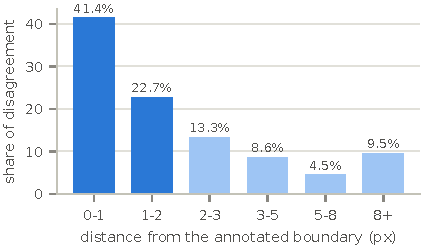
\includegraphics[width=0.62\textwidth]{figures/fig_rim.pdf}
\caption{Where matched masks disagree with their annotations: the share of disagreeing pixels as a
function of their distance from the annotated boundary, over 124 matched pairs.
\generatedby{book/make\_book\_figures.py:fig\_rim}}
\label{fig:post-rim}
\end{figure}

An oracle converted this observation into a score. Removing all of the disagreement within two
pixels of the boundary would raise SQ from about 0.68 to 0.855, and PQ from 0.435 to 0.547 at the
same recognition quality. Removing the disagreement deeper than three pixels instead would raise PQ
only to 0.469. The rim is therefore worth about three times as much as the interior. The deepest band
also showed an unbalanced pattern: beyond eight pixels from the boundary, the model added 5,062
pixels that no annotator drew and missed only 1,384, an over-prediction of 3.7 to 1, whereas every
other band was close to balanced.

How much of the error at the rim can any method remove? The annotators themselves disagree about the
rim. In exp088 we built one mask per filament from the pixel-wise majority of the annotators, and
scored it against \emph{every} annotator of the photograph. It reached a mean IoU of about 0.81, and
the best single annotator's mask reached about 0.80. Our own masks reached 0.68 on the same
photographs. The measured headroom for work on the boundary is therefore roughly the interval from
0.68 to 0.81 in SQ, rather than from 0.68 to 1.

At one point our strategy notes derived an ``SQ ceiling of about 0.82'' by modelling each annotator
as a noisy copy of a hidden true boundary. That model was never tested, and the notes now mark it as
a hypothesis. The measurement of exp088, which scores real masks against real annotators, is the one
to use.

\section{Learned refiners}\label{sec:post-refiners}
The analysis of the rim made a strong case for a \keyterm{refiner}: a second network that takes a
crop of the photograph together with a coarse mask, and redraws the boundary pixel by pixel instead
of trimming every mask by the same amount~\citep{cheng2020cascadepsp,pointrend}. We trained three refiners (Figure~\ref{fig:post-refiner}).

\begin{figure}[t]
\centering
\begin{tikzpicture}[
  st/.style={box=#1, text width=2.35cm, minimum height=1.0cm, font=\sffamily\scriptsize,
             execute at begin node={\hyphenpenalty=10000}}]
  \node[st=inkmuted] (syn) at (0,0.75) {synthetic pairs: annotation dilated, shifted and smoothed};
  \node[st=inkmuted] (real) at (0,-0.75) {real pairs: detector masks matched to annotations};
  \node[st=vizblue, text width=2.6cm, minimum height=1.6cm] (net) at (3.7,0)
       {refiner U-Net on a 256 px native crop; inputs: photograph and coarse mask};
  \node[st=vizorange] (out) at (7.3,0) {refined mask, pasted back at native resolution};
  \draw[flow] (syn.east) -- (net.west |- 0,0.35);
  \draw[flow] (real.east) -- (net.west |- 0,-0.35);
  \draw[flow] (net) -- (out);
  \node[note, anchor=west, text width=2.6cm, align=left] at (8.75,0.75)
       {exp008/009: own task 0.72\,$\to$\,0.85 IoU; PQ $-0.008$};
  \node[note, anchor=west, text width=2.6cm, align=left] at (8.75,-0.75)
       {exp012/018: 0.61\,$\to$\,0.63 IoU; PQ $-0.031$};
\end{tikzpicture}
\caption{The mask refiners. The same crop-level U-Net was trained on synthetic damage and on real
detector errors. The first learned its own task and still lowered PQ; the second learned almost
nothing and lowered it further. \drawnin{book/chapters/ch09\_postprocessing.tex}}
\label{fig:post-refiner}
\end{figure}

\subsection{Training on synthetic damage}\label{sec:post-synthetic}
The first refiner (exp008 and exp009) was trained on pairs made by damaging the annotations: we
dilated, shifted and smoothed them to imitate the errors that we had measured in the detector's
masks. The refiner learned this task well, raising the IoU on its own validation crops from 0.72 to
0.85 after 138 minutes of training on eight TPU cores. Applied to the detector's real output,
however, it lost:
\begin{center}\small
\begin{tabular}{@{}lccccc@{}}
\toprule
configuration & PQ & SQ & TP & FP & FN \\
\midrule
detector, masks untouched & 0.4169 & 0.671 & 829 & 514 & 496 \\
detector and refiner at threshold 0.6 & 0.4322 & 0.673 & 847 & 467 & 478 \\
\textbf{detector and one-pixel erosion} & \textbf{0.4404} & \textbf{0.684} & 845 & 456 & 480 \\
\bottomrule
\end{tabular}
\end{center}
The refiner improved on the untouched masks, but it lost by 0.008 to an operation with no parameters
at all, and on the leaderboard it appeared as 0.35 against 0.36. Our diagnosis was that the
synthetic damage matched the detector's errors in \emph{severity}, that is, in the average IoU of the
damaged masks, but not in \emph{character}. Real errors are correlated with the content of the
image, for example with faint filaments near the limb, or with neighbouring objects that compete for
the same prototypes. A hand-written corruption does not reproduce these correlations.

A small follow-up experiment taught us something about reading numbers. The SQ of the refined masks
(0.673) was lower than that of the eroded masks (0.684), which suggested that the refined masks were
still too wide and that eroding them would help. Eroding the refined masks cost six hundredths. The
refined masks had roughly the right size and the wrong shape. We had read a single scalar difference
as evidence about the \emph{direction} of an error, and it carried no such information.

\subsection{Training on real errors}\label{sec:post-real}
The obvious remedy was to train on real errors. In exp011 we ran the detector over the training
photographs and harvested 3,429 matched pairs of predicted and annotated masks. A refiner trained on
them (exp012 and exp018) raised the validation IoU from 0.611, the IoU of its input masks, to 0.634
at the second epoch, and never improved after that, although its training loss kept falling: it
was memorising the training crops. Scored on the detector's output, it lost 0.031 PQ, because it
rewrote about a third of each mask, and rewrote it wrongly.

\subsection{A second refiner and a resampling artefact}\label{sec:post-v2}
A later refiner (exp091 to exp094), trained on 7,442 harvested proposals, reported an improvement
in IoU of $+0.0118$ on its crops. In exp094 we found that the improvement had been produced by the
measurement itself. Scoring masks at the resolution of the crops, after resampling
them with nearest-neighbour interpolation, raises their IoU by $+0.0117$ even when no model is
involved. When we pasted the refined masks back into the photographs and scored them at the native
resolution, they were slightly \emph{worse} than the originals ($-0.0023$).

The general rule is that we should measure where the metric measures. The competition scores masks
at $2048\times2048$ pixels, after they have been painted into a disjoint set. A score computed at
another resolution, on crops, or on a filtered subset of the instances can change for reasons that
have nothing to do with the method, so every candidate method should be pasted back, painted and
scored with the official metric at the native resolution before its number is believed.

\section{Corrections without training}\label{sec:post-free}
If a network cannot learn to correct the boundary, perhaps a fixed rule can. We tried four
corrections that need no training.

\paragraph{A higher cut on the mask field (exp017).} YOLO turns its continuous field of mask logits
into a binary mask by thresholding it at zero. Raising the threshold moves each boundary inward by an
amount that depends on the local gradient of that mask's own logits. This gives a continuous,
per-instance trim, which the one-pixel erosion is not. As a mechanism it works: with no erosion, a
cut at a logit of 0.9 recovered 0.018 of the 0.023 that erosion recovers. However, it never beat
erosion, and the two do not combine, because they make the same correction. The variation of the
trim from one mask to another did not correlate with how much each mask needed to be trimmed.

\paragraph{Snapping to the intensity edge (exp029).} A filament is dark and the disk is bright, so
the boundary seems to be physically present in the photograph, and one could pull each mask onto it
without any learning, much as an active contour~\citep{kass1988} is pulled onto the edges of an
image. On a synthetic filament drawn as a clean step in intensity, snapping raised the IoU of a mask
that was too wide from 0.80 to 0.9995. On real photographs it destroyed the masks, and the more of
the boundary it was allowed to move, the worse the result. The table also includes a guided
filter~\citep{he2013guided}, which smooths a mask along the edges of the photograph; it changed
almost nothing:
\begin{center}\small
\begin{tabular}{@{}lccc@{}}
\toprule
method & PQ & SQ & RQ \\
\midrule
untouched & 0.4274 & 0.678 & 0.631 \\
guided filter & 0.4276 & 0.678 & 0.631 \\
intensity snap, band of 2 px & 0.3933 & 0.654 & 0.601 \\
intensity snap, band of 3 px & 0.3491 & 0.633 & 0.552 \\
intensity snap, band of 5 px & 0.2739 & 0.621 & 0.441 \\
\bottomrule
\end{tabular}
\end{center}
Figure~\ref{fig:post-profile} shows why. A real filament has no edge. It fades into the disk over
several pixels, and the annotated boundary is a judgement about where the fading stops counting as
filament. The synthetic test had a hard edge built into it, and the existence of such an edge was the
very assumption that the test was supposed to check.

\begin{figure}[t]
\centering
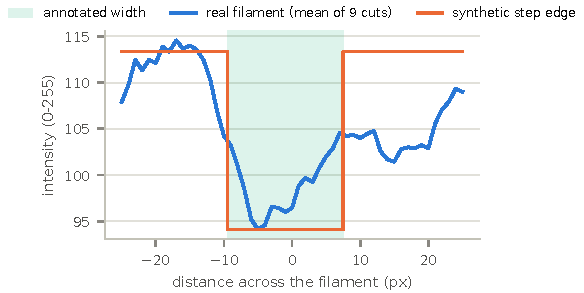
\includegraphics[width=0.66\textwidth]{figures/fig_profile.pdf}
\caption{The intensity across a real annotated filament (the mean of nine cuts perpendicular to its
axis), compared with the step edge that a synthetic test assumed. The real profile fades over several
pixels, so no particular intensity level marks the annotated width.
\generatedby{book/make\_book\_figures.py:fig\_profile}}
\label{fig:post-profile}
\end{figure}

\paragraph{A foundation model (exp066).} We prompted SAM2~\citep{ravi2024sam2}, a general-purpose
segmentation model that extends Segment Anything~\citep{sam}, with the box of each detection, with and without three points inside the mask, and
asked it to redraw the mask. On 24 validation photographs its masks scored 0.358, against 0.459 for
the unchanged masks.

\paragraph{Borrowing another model's boundary (exp072 and exp075).} For each detection that a second
model had also found, we replaced the mask by the second model's mask, or by the intersection or union
of the two. All 640 substitutions lowered the score, which ranged from 0.4529 to 0.4538 against
0.4559 without them.

\subsection{Five failures and an overreach}\label{sec:post-overreach}
By this point five methods had failed to improve the boundary, each approaching it from a different
direction: the refiner trained on synthetic damage, the refiner trained on real errors, the higher
logit cut, the intensity snap, and a crop verifier that we describe in Chapter~\ref{ch:recall}. Our
notes then drew a sweeping conclusion: the annotated boundary is one person's judgement, it cannot be
recovered from the image, and therefore \emph{no} post-processing method can reach it.

The measurements were sound, but the conclusion went beyond them. The failure of five particular
formulations is evidence about those formulations. It does not show that every formulation must
fail, and the notes later marked this reasoning as an unproven generalisation. An independent review
of our later work on repairs made the same point more sharply. Of the sixteen repair approaches on
our list at that time, three had been tested directly, three partially, and ten not at all, and the
review observed that ``demotion by a shared precondition is not refutation''. The next two sections
describe the more careful approach that came out of this correction.

\section{Structural repairs}\label{sec:post-structure}
Chapter~\ref{ch:metric} showed that PQ rewards a prediction that crosses the matching threshold far
more than it rewards an improvement to a mask that already matches. A prediction with an IoU of 0.49
adds nothing to the numerator, whereas at 0.51 it adds 0.51 (Section~\ref{sec:metric-leverage}). The
useful question for post-processing is therefore which masks lie just below the threshold, and what
would push them over it. Improving every mask a little is worth far less.

\subsection{What the near misses look like}\label{sec:post-nearmiss}
In exp105 we built, for each annotation record, the bipartite graph whose nodes are the predicted and
annotated masks and whose edges connect overlapping pairs, and we classified the connected components
of this graph, in the spirit of the error analyses that \citet{hoiem2012} and \citet{bolya2020tide}
made for object detectors:
\begin{center}\small
\begin{tabular}{@{}lcc@{}}
\toprule
component & count & with IoU in $[0.4, 0.5)$ \\
\midrule
one prediction, one filament (1:1) & 953 & \textbf{55} \\
several predictions, one filament (fragments) & 29 & 5 \\
one prediction, several filaments (merge) & 24 & 5 \\
several predictions and several filaments & 4 & 1 \\
filament with no overlapping prediction & 286 & -- \\
prediction with no overlapping filament & 211 & -- \\
\bottomrule
\end{tabular}
\end{center}
Most of the near misses (55 of 66) were simple one-to-one pairs whose masks had the wrong shape,
rather than tangles of splits and merges. These 55 masks were \emph{under}-segmented: the median
near miss lacked 575 annotated pixels and had only 139 extra ones. In exp108 we asked where the
missing pixels were (Figure~\ref{fig:post-nearmiss}). For the near misses, 59\% of the missing
pixels lay beyond the end of the mask along its axis, at a median distance of 10.9 pixels, on bodies
with a half-width of only about 2.2 pixels. For healthy matches, by contrast, 76\% of a much smaller
deficit lay within three pixels of the mask. The near misses were therefore mostly
\keyterm{truncated}, that is, cut short, rather than drawn too thin.

\begin{figure}[t]
\centering
\begin{tikzpicture}[
  truth/.style={line width=7pt, line cap=round, draw=inkmuted!45},
  pred/.style={line width=#1, line cap=round, draw=vizorange},
  pred/.default=4pt]
  % (a) healthy: slightly thin everywhere
  \draw[truth] (0,0) .. controls (0.8,0.5) and (1.6,0.5) .. (2.5,0.1);
  \draw[pred=5pt] (0.05,0.03) .. controls (0.8,0.5) and (1.6,0.5) .. (2.45,0.12);
  % (b) truncated: the mask stops short of the filament's end
  \begin{scope}[xshift=3.6cm]
    \draw[truth] (0,0) .. controls (0.8,0.5) and (1.6,0.5) .. (2.5,0.1);
    \draw[pred=5pt] (0,0) .. controls (0.45,0.3) and (0.9,0.4) .. (1.35,0.38);
    \draw[<->, line width=0.5pt, draw=inkprimary] (1.45,0.6) -- node[note, above=1pt] {10--30 px missing} (2.45,0.35);
  \end{scope}
  % (c) merge: one mask over two filaments
  \begin{scope}[xshift=7.2cm]
    \draw[truth] (0,0) .. controls (0.5,0.3) and (0.9,0.35) .. (1.2,0.3);
    \draw[truth] (1.35,0.28) .. controls (1.7,0.2) and (2.1,0.05) .. (2.5,-0.1);
    \draw[pred=5pt] (0,0) .. controls (0.5,0.3) and (0.9,0.35) .. (1.2,0.3) -- (1.35,0.28) .. controls (1.7,0.2) and (2.1,0.05) .. (2.5,-0.1);
  \end{scope}
  \node[note] at (1.25,-0.55) {(a) healthy match:\\ marginally thin at the rim};
  \node[note] at (4.85,-0.55) {(b) near miss:\\ truncated along the axis};
  \node[note] at (8.45,-0.55) {(c) merge: one mask\\ covers two filaments};
  \draw[truth] (10.35,0.45) -- (10.75,0.45); \node[note, anchor=west] at (10.85,0.45) {annotation};
  \draw[pred] (10.35,0.05) -- (10.75,0.05); \node[note, anchor=west] at (10.85,0.05) {prediction};
\end{tikzpicture}
\caption{Three shapes of error. Healthy matches are slightly too thin near the boundary (a). Most near
misses are truncated: the mask stops well short of the end of the filament (b). A smaller group
merges two annotated filaments into one mask (c). \drawnin{book/chapters/ch09\_postprocessing.tex}}
\label{fig:post-nearmiss}
\end{figure}

\subsection{Triggers: can we tell which masks to repair?}\label{sec:post-triggers}
A repair needs a \keyterm{trigger}, an observable signal that indicates which masks need it, because
at test time we do not know which masks lie just below the threshold. Every trigger that we tried was
weak:
\begin{center}\small
\begin{tabularx}{\textwidth}{@{}lXc@{}}
\toprule
experiment & signal & AUC \\
\midrule
exp105c & mask geometry: elongation, solidity, variation of width, and their combination & 0.42--0.55 \\
exp105c & narrow neck: minimum width over median width (for merges) & 0.71 \\
exp106 & the semantic model's support in a ring around the mask & 0.40--0.64 \\
exp107 & disagreement between two YOLO architectures & 0.57--0.60 \\
exp109 & evidence in a cone ahead of the mask's endpoint & near chance \\
exp110--112 & darkness and ridge orientation along the best path ahead & 0.52--0.62 \\
exp111 & profile of the width along the axis (for merges) & 0.72--0.81 \\
\bottomrule
\end{tabularx}
\end{center}
The \keyterm{AUC}, the area under the receiver operating characteristic
curve~\citep{hanley1982,fawcett2006}, is the probability
that a randomly chosen mask needing repair receives a higher score from the trigger than a randomly
chosen mask that does not; it is 0.5 for a random trigger and 1.0 for a perfect one. Even the best
signal, the width profile with an AUC of 0.81, ran into a \keyterm{precision wall}. There were 24
merged masks among 882, a base rate below 3\%. At any threshold that caught a useful share of the 24,
the healthy masks caught alongside them outnumbered them several times over. Experiment exp108 also
explained why the triggers based on a ring around the mask had failed: they sampled a band four pixels
wide around the mask, whereas the missing pixels of a truncated mask lay 10 to 30 pixels beyond its
end.

\section{A protocol for repair experiments}\label{sec:post-protocol}
We had rejected several of these repair ideas because their triggers failed. That was an error of
sequencing: a failed trigger tells us nothing about whether the repair itself is worth anything. The
testing manual that we adopted fixed the order of the questions (Figure~\ref{fig:post-protocol}),
and we introduced it in general terms in Section~\ref{sec:val-oracles}. Here we apply it.

\begin{figure}[t]
\centering
\begin{tikzpicture}[
  st/.style={box=#1, text width=3.0cm, minimum height=1.6cm, font=\sffamily\scriptsize,
             execute at begin node={\hyphenpenalty=10000}}]
  \node[st=vizblue] (a) at (0,0) {\textbf{\color{inkprimary}1. ceiling}\\ an oracle repair that reads the annotations: the family's maximum gain};
  \node[st=vizaqua] (b) at (4.7,0) {\textbf{\color{inkprimary}2. operator}\\ the real repair, told by an oracle exactly which masks to act on};
  \node[st=vizorange] (c) at (9.4,0) {\textbf{\color{inkprimary}3. gate}\\ the real trigger that chooses the masks; its break-even rate};
  \draw[flow] (a) -- node[note, above=1pt] {worth it?} (b);
  \draw[flow] (b) -- node[note, above=1pt] {recovers it?} (c);
  \node[note, text width=3.1cm, align=center] at (0,-1.3) {split: +0.0223\\ lateral growth: +0.0189};
  \node[note, text width=3.1cm, align=center] at (4.7,-1.3) {neck cut: +0.0028 (13\%)\\ dilation: +0.0064 (34\%)};
  \node[note, text width=3.1cm, align=center] at (9.4,-1.3) {dilation needs a gate with\\ TPR / FPR $>$ 3.9};
\end{tikzpicture}
\caption{The protocol for testing a family of repairs. Each step answers one question, and it is run
only if the previous step says that the family is worth pursuing. The numbers come from exp113, exp114
and exp117. \drawnin{book/chapters/ch09\_postprocessing.tex}}
\label{fig:post-protocol}
\end{figure}

\subsection{Step 1: ceilings}\label{sec:post-ceilings}
In exp113 we measured, for each family of repairs, how much a perfect repair could gain if the
annotations were allowed to guide it. Splitting merged masks along the true boundary was worth
$+0.0223$. Growing truncated masks to their true extent was worth $+0.0325$ in total, divided into
lateral growth ($+0.0189$) and axial growth ($+0.0181$), which overlap. Joining fragments was worth
$+0.0116$. Every family passed this first step, and three of them could in principle have lifted our
baseline of 0.4559 above 0.472, the validation score that at the time corresponded to a public score
of 0.40. An oracle ceiling of this kind is an upper bound for research purposes; it can never be
submitted.

\subsection{Step 2: operators under a perfect gate}\label{sec:post-operators}
Given the exact list of masks to repair, how much of the ceiling does a real repair operator recover
(Figure~\ref{fig:post-ceilings})? For splitting, the best rule, a cut across the narrowest point of
the mask's interior, recovered 13\% of the ceiling ($+0.0028$). It rescued 22 of the 40 filaments
that a perfect split rescues, and it damaged 6 healthy matches. A watershed
split~\citep{vincent1991} lost outright. For
growth, the result was surprising: plain dilation, which reads no evidence from the image at all,
beat every growth rule that was guided by the image. Two steps of dilation recovered 34\% of the
lateral ceiling ($+0.0064$), about twice as much as the best grower guided by darkness. Axial growth
along rays from the endpoint of the mask recovered at most 7\% of its ceiling.

\begin{figure}[t]
\centering
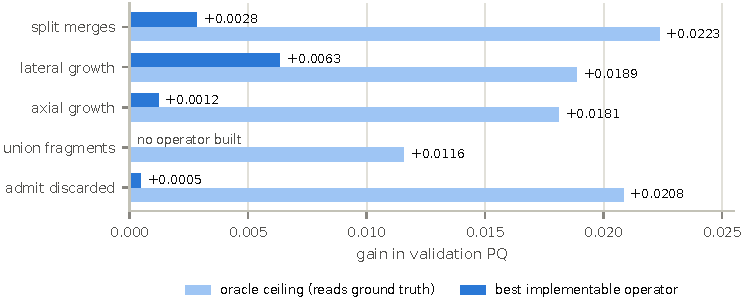
\includegraphics[width=\textwidth]{figures/fig_ceilings.pdf}
\caption{The oracle ceiling of each family of repairs (light), against the best operator that can be
implemented, given a perfect gate (dark). The last row is the admission of discarded candidates
described in Chapter~\ref{ch:recall}. \generatedby{book/make\_book\_figures.py:fig\_ceilings}}
\label{fig:post-ceilings}
\end{figure}

\subsection{Step 3: what a gate must achieve}\label{sec:post-gate}
Comparing an operator with and without its perfect gate reveals what a real gate would have to do.
One step of dilation, applied only to the 55 near-miss masks, pushed 11 of them over the threshold
and harmed none. Applied to all 953 one-to-one masks, it pushed the same 11 over, but it also pushed
43 healthy matches \emph{below} the threshold. Every gain came from the near misses and every loss
from the other masks. Suppose that a gate fires on a fraction TPR of the near misses and on a fraction
FPR of the healthy masks. Since each crossing in either direction changes the score by roughly the
same amount, the expected change is proportional to $11\,\mathrm{TPR} - 43\,\mathrm{FPR}$, and
breaking even requires
\begin{equation}
\frac{\mathrm{TPR}}{\mathrm{FPR}} > \frac{43}{11} \approx 3.9 .
\label{eq:post-gate}
\end{equation}
No trigger in the table of Section~\ref{sec:post-triggers} came close to this ratio at a useful
true-positive rate.

The protocol therefore asks three questions in a fixed order. We first measure the family's
ceiling with an oracle, then measure how much of it a real operator recovers under a perfect gate,
and only then build the real trigger, whose break-even rate we compute from the gated and ungated
runs. A trigger that fails tells us nothing about the value of the repair, and a large ceiling tells
us nothing about whether any practical operator can reach it.

\section{What post-processing could do}\label{sec:post-summary}
Measured carefully, post-processing earned us one large gain and many small losses. The one-pixel
erosion corrected a systematic, uniform bias, and a uniform correction needs no trigger. Every method
that required deciding \emph{which} masks to change stalled, either at the operator or at the gate.
Two facts about the data explain much of this. The error lies mostly at the rim, where the annotators
also disagree, and the near misses are truncations whose missing pixels leave little trace in the
image around the mask. These results do not show that the problem is unsolvable; they show that the
formulations we tested were weak. Our response was to look for a model whose masks needed less repair
in the first place (Chapters~\ref{ch:transformers} and~\ref{ch:training}).

\section*{Exercises}
\begin{exercise}{The rim oracle}
Using Figure~\ref{fig:post-rim}, estimate the gain in SQ from removing all of the disagreement within
one pixel of the boundary, assuming that the disagreement averages 0.472 times the intersection.
Compare your estimate with the gain that the one-pixel erosion actually delivered.
\end{exercise}

\begin{exercise}{Severity is not character}
Write a synthetic damage model whose mean IoU with the annotations is exactly the detector's 0.61.
Propose two statistics of the detector's real errors that your model would fail to reproduce, and
explain how you would measure them on the harvested pairs.
\end{exercise}

\begin{exercise}{Snapping on a real profile}
Take the real profile of Figure~\ref{fig:post-profile}. For each intensity level between its minimum
and its background value, compute the width at which the profile crosses that level. Which level
reproduces the annotated width, and does the same level work for a second filament?
\end{exercise}

\begin{exercise}{The break-even ratio of a gate}
Derive Equation~\eqref{eq:post-gate}, stating the assumption that you make about the value of each
crossing. If each harmful crossing also lowers the SQ of the healthy mask, does the required ratio
rise or fall?
\end{exercise}

\begin{exercise}{The precision wall}
A trigger has an AUC of 0.81 on 24 positives among 882 masks. Assume that the scores of both groups
are Gaussian with equal variance. Find the separation between the two means that gives an AUC of
0.81, and compute the precision at a threshold that catches half of the positives.
\end{exercise}

\chapter{Finding What the Detector Missed}\label{ch:recall}

\section{Introduction}\label{sec:recall-intro}
\epigraph{Far better an approximate answer to the right question, which is often vague, than an exact
answer to the wrong question, which can always be made precise.}{John Tukey, \emph{The Future of Data
Analysis} \citeyearpar[p.~13]{tukey1962}}

At the best operating point of our YOLO pipeline, about a third of the annotated filaments went
unmatched: there were 465 false negatives against 860 true positives. Recall is therefore where most
of the missing score lies. However, a filament can be missed for three quite different reasons, and
each calls for a different remedy.
\begin{itemize}[leftmargin=*,itemsep=2pt]
\item The detector never proposed anything at that location. The remedy is a better detector, or a
new source of proposals.
\item The detector proposed a good mask, and the confidence threshold discarded it. The remedy is a
\keyterm{verifier} that rescues good candidates with low confidence.
\item The detector proposed a mask on the right object, but the mask was too poor to reach an IoU of
0.5. The remedy is better boundaries (Chapter~\ref{ch:post}).
\end{itemize}

In Sections~\ref{sec:recall-orphans} and~\ref{sec:recall-stages} we measure how often each of these
cases occurs. Section~\ref{sec:recall-arith} works out how accurate a verifier must be before it can
help, and Section~\ref{sec:recall-verifiers} describes the verifiers that we built.
Sections~\ref{sec:recall-physics} and~\ref{sec:recall-semantic} try two other sources of evidence,
the physics of the image and a semantic segmentation model, and Section~\ref{sec:recall-summary}
summarises what we learned.

\section{Seen, unseen, or disbelieved?}\label{sec:recall-orphans}
Our first measurements concerned the false positives. In exp014 we called a prediction an
\keyterm{orphan} if no annotated filament overlapped it even at an IoU of 0.10. Against a given
annotator, 19.8\% of the detector's predictions were orphans. On the photographs with several
annotators, 19.4\% of one annotator's filaments were orphans with respect to a second annotator. In
other words, the detector's unacknowledged predictions occurred at the same rate as one expert's
unacknowledged filaments occur for another expert. More directly, 87 of the detector's orphans had
been drawn by a \emph{different} annotator of the same photograph.

Our notes then extended this conclusion to the misses, claiming that they too were mostly caused by
label noise. That extension was wrong, as exp016 showed by examining the whole pool of candidates,
down to a confidence of 0.05, instead of only the predictions that were emitted:
\begin{center}\small
\begin{tabular}{@{}lcc@{}}
\toprule
validation filaments (1,325) & count & share \\
\midrule
some candidate in the pool matches it at IoU 0.5 & 1,102 & 83.2\% \\
\quad of which already above the threshold of 0.35 & 797 & \\
candidates in the pool overlap it, but never reach IoU 0.5 & 195 & 14.7\% \\
no candidate in the pool touches it at all & 28 & 2.1\% \\
\bottomrule
\end{tabular}
\end{center}
Only 2.1\% of the filaments were invisible to the detector. Most of the misses had been \emph{seen
and disbelieved}: 305 filaments had a matching candidate that the threshold discarded. A result
about the false positives had been generalised to the false negatives, where it did not hold.

\section{The error, stage by stage}\label{sec:recall-stages}
We made the most careful version of this measurement later, on the two-model YOLO ensemble. In exp129
and exp132 we asked, for every annotated filament, how good the best candidate anywhere in the pool
was, with no confidence floor, no minimum area and no painting, but with the masks eroded as the
pipeline emits them (Figure~\ref{fig:recall-stages}).

\begin{figure}[t]
\centering
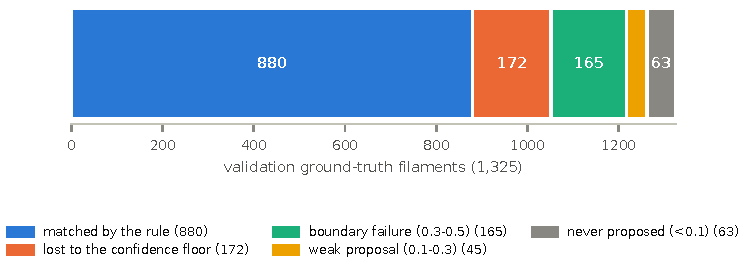
\includegraphics[width=\textwidth]{figures/fig_stages.pdf}
\caption{Every validation filament, classified by the best candidate that the pool holds for it. Most
filaments are matched by the deployed rule. The next largest groups are those whose good candidate
was discarded by the confidence floor, and those whose candidate lies on the right object but with a
boundary too poor to match. Few filaments were never proposed.
\generatedby{book/make\_book\_figures.py:fig\_stages}}
\label{fig:recall-stages}
\end{figure}

Of the filaments that the deployed rule missed, 172 had a good candidate below the confidence floor,
165 had a candidate on the right object with an IoU between 0.3 and 0.5, 45 had only a weak
candidate, and 63 (4.8\% of all filaments) were never proposed. Oracles on the uneroded pool put a
value on each remedy. Fixing the emission perfectly, that is, admitting exactly the good candidates
that the floor discarded, would raise validation PQ by $+0.050$. Fixing the boundaries of the group
with IoU between 0.3 and 0.5 would add $+0.059$, and doing both would add $+0.101$.

A companion audit, exp130, asked why the good candidates were lost. Of the 203 filaments whose best
raw candidate had an IoU above 0.5 but which nevertheless ended up unmatched, 168 (83\%) fell below
the confidence floor, 13 fell below the minimum area, 12 were destroyed by the erosion, and 10 lost
their pixels to a mask with a higher score during painting. The confidence floor was therefore the
stage that mattered.

This analysis corrected an earlier error. Before exp129, our notes had stated that 284 missed
filaments ``have zero overlap with any prediction'', and had concluded from this that the problem
was entirely one of detection. The 284 filaments had no overlap with the \emph{emitted} predictions,
which are what remains after the confidence floor has already discarded much of the evidence. In the
full pool, only 65 of them had never been proposed. Whenever we quote a number, we must know at which
stage of the pipeline it was measured.

\section{The arithmetic of admitting candidates}\label{sec:recall-arith}
Suppose that a verifier admits $k$ discarded candidates that are correct, with a mean IoU of $q$,
and $m$ that are not. Equation~\eqref{eq:metric-breakeven} of Chapter~\ref{ch:metric} says that the
score improves only if the verifier's precision exceeds $\PQ/(2q)$. Figure~\ref{fig:recall-breakeven}
plots this bar as a function of $q$.

\begin{figure}[t]
\centering
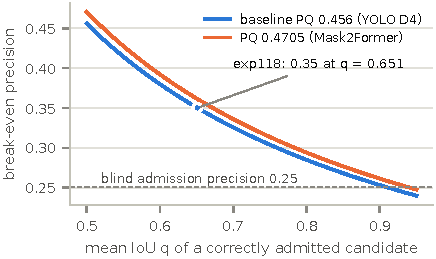
\includegraphics[width=0.62\textwidth]{figures/fig_breakeven.pdf}
\caption{The precision that a verifier needs before the candidates it admits raise PQ, as a function
of the mean IoU $q$ of the correct admissions. Admitting candidates blindly, by lowering the threshold,
reaches a precision of only about 0.25. \generatedby{book/make\_book\_figures.py:fig\_breakeven}}
\label{fig:recall-breakeven}
\end{figure}

In exp118 we measured both sides of this inequality on the pool of the YOLO ensemble, which held 601
candidates with confidences between 0.10 and the floor of 0.35. Lowering the floor blindly always
lowered the score:
\begin{center}\small
\begin{tabular}{@{}cccccc@{}}
\toprule
floor & PQ & added TP & added FP & precision of the additions \\
\midrule
0.35 (deployed) & 0.4559 & -- & -- & -- \\
0.30 & 0.4501 & 32 & 95 & 0.25 \\
0.25 & 0.4421 & 63 & 205 & 0.24 \\
0.20 & 0.4260 & 89 & 365 & 0.20 \\
0.10 & 0.3969 & 109 & 634 & 0.15 \\
\bottomrule
\end{tabular}
\end{center}
An oracle that admitted exactly the right candidates reached 0.4767, a gain of $+0.0208$, by admitting
132 candidates that recovered 120 misses with a mean IoU of 0.651. At this value of $q$,
Equation~\eqref{eq:metric-breakeven} sets the bar at a precision of 35\%, but a precision of 35\%
only breaks even. To reach 0.472, the verifier needed a precision of about 50\% at around 120
admissions, whereas blind admission achieved 24 to 25\%. A useful verifier therefore had to roughly
double the precision of the candidates that it chose.

\section{Verifiers}\label{sec:recall-verifiers}
A \keyterm{verifier} is a second model that re-scores the detector's candidates, using evidence that
the detector's confidence does not already contain. We built several.

\subsection{Hand-made features}\label{sec:recall-features}
Our first verifier was a gradient-boosted classifier~\citep{friedman2001} over four shape features: area, elongation,
distance from the limb, and solidity. We trained it with the photographs grouped, so that no
photograph appeared in both the training and the validation folds. It lost to the raw confidence by
0.017. A re-ranker built on fourteen cuts through each mask's field of logits ranked the candidates
slightly better than the confidence did (an average precision of 0.7248 against 0.7150), yet even its
most conservative promotion added 23 false positives and no true ones.

Later screens on the ensemble's pool found no single feature that could verify a discarded
candidate. The best was the detector's own score, with an AUC of 0.64, followed by the distance from
the limb, with an AUC of 0.60; candidates near the centre of the disk were more often real. A logistic
regression~\citep{murphy} over nine features, fitted out of fold, recovered 8\% of the admission ceiling
($+0.0017$). Gradient boosting on the same features memorised the 132 positive examples and lost.
Whether a second architecture also proposed the candidate was the best single feature we found, with
an AUC of 0.688, and it still did not yield an operating point with a positive gain.

\subsection{The crop verifier and the wrong question}\label{sec:recall-crop}
In exp025 to exp027 we trained a small convolutional network, with 827,000 parameters, on 13,413 crops
of $128\times128$ pixels. Each crop had two channels: the photograph and the proposed mask. For
candidates with confidence below 0.30, its average precision was 0.576, against 0.455 for the
detector's confidence and a base rate of 0.344. Of its top 100 candidates in this range, 72\% were
real filaments. Yet when we used it as an emission rule, it added 100 true positives at the cost of
496 false positives, a precision of 17\%.

The gap between 72\% and 17\% was caused by a decision about labels. We had labelled a crop as
positive if \emph{any} annotator of the photograph had drawn a filament there, reasoning that
labelling against a single annotator would teach the model to call another annotator's filament a
mistake. But PQ scores each annotation record separately, against \emph{one} annotator
(Figure~\ref{fig:recall-labels}). The verifier had learned to answer the question ``would somebody
draw this?'', whereas the metric asks ``did this person draw it?''.

\begin{figure}[t]
\centering
\begin{tikzpicture}[
  panel/.style={draw=inkmuted, line width=0.6pt, fill=gridline!40, minimum width=3.2cm,
                minimum height=1.9cm, rounded corners=2pt},
  truth/.style={line width=6pt, line cap=round, draw=inkmuted!55},
  cand/.style={line width=1.2pt, draw=vizorange, dash pattern=on 3pt off 1.5pt},
  tag/.style={font=\sffamily\scriptsize\bfseries, text=white, fill=#1, rounded corners=1.5pt,
              inner sep=2.5pt}]
  \foreach \px/\ttl in {0/{record of annotator A}, 3.9/{record of annotator B}}{
    \node[panel] at (\px,0) {};
    \node[title] at (\px,1.2) {\ttl};
  }
  % annotator A drew both filaments; annotator B drew only the upper one
  \draw[truth] (-1.2,0.45) .. controls (-0.5,0.7) and (0.4,0.3) .. (1.2,0.5);
  \draw[truth] (-1.0,-0.45) .. controls (-0.4,-0.25) and (0.3,-0.55) .. (1.0,-0.35);
  \begin{scope}[xshift=3.9cm]
    \draw[truth] (-1.2,0.45) .. controls (-0.5,0.7) and (0.4,0.3) .. (1.2,0.5);
  \end{scope}
  % the same candidate on the lower filament in both records
  \foreach \px in {0,3.9}{
    \begin{scope}[xshift=\px cm]
      \draw[cand] (-1.05,-0.5) .. controls (-0.4,-0.3) and (0.3,-0.6) .. (1.05,-0.4) -- (1.05,-0.28) .. controls (0.3,-0.48) and (-0.4,-0.18) .. (-1.05,-0.38) -- cycle;
    \end{scope}
  }
  \node[tag=vizblue] at (0,-1.25) {per record: positive};
  \node[tag=vizorange!85!black] at (3.9,-1.25) {per record: negative};
  \node[box=inkmuted, text width=2.9cm, font=\sffamily\scriptsize] at (8.0,0.25)
       {``any annotator'' label: \textbf{positive} for both records};
  \node[note, text width=3.2cm] at (8.0,-0.85) {PQ scores each record on its own, so one admission is a TP in A and an FP in B};
\end{tikzpicture}
\caption{Why a verifier must be labelled per record. The dashed candidate lies on a filament that
annotator A drew and annotator B did not. Labelled ``positive if any annotator drew it'', the
candidate teaches the verifier a question that PQ never asks.
\drawnin{book/chapters/ch10\_recall.tex}}
\label{fig:recall-labels}
\end{figure}

The lesson is general. Before choosing the labels for a model, we should write down the exact
question that the metric asks of each prediction, and check that the training objective asks the same
question. Here the metric asks, for each annotation record, whether this candidate matches this
annotator's filament with an IoU above one half.

We also used the mistake as a probe of the leaderboard. If the test labels were a consensus of several
annotators, or otherwise more inclusive than those of a single annotator, then the crop verifier's
high-recall rule would transfer to the leaderboard better than its validation score suggested. We
submitted it as exp028: it emitted 1,624 instances and scored 0.041 \emph{worse} on validation. It
appeared on the leaderboard as 0.32, which is what the usual offset between validation and the
leaderboard predicts, so the test labels behave like the validation labels
(Section~\ref{sec:val-rejected}).

\subsection{The crop verifier with the right labels}\label{sec:recall-crop-fixed}
In exp134 we repeated the idea with the labels corrected. There was one example for each combination
of photograph, record and proposal, and it was positive only if the proposal matched a filament in
that record. We trained the network on 5,281 crops harvested from the training photographs, of which
19\% were positive. The inputs were well formed, and the ceiling was real: 168 of the 172 filaments
lost to the confidence floor had a proposal with an IoU above 0.5 among the crops. The model did not
learn. Its average precision on validation wandered between 0.19 and 0.25 for twenty epochs, against a
base rate of 0.18, and its loss stayed at the value that a random classifier achieves. Every admission
rule based on it lost. Two simple physical features, the contrast in darkness between the inside and
the outside of the mask, and the mask's area, were also at chance, with AUCs of 0.53 and 0.50.

Our interpretation is that, for these candidates, the detector's low confidence reflects a real
uncertainty: within a crop of 128 pixels, a real filament under a low-confidence proposal does not
look different from a false one. This statement is about the formulations we tested, namely crops of
this size and features of this kind, and we do not claim more than that.

\section{Physics and classical vision}\label{sec:recall-physics}
If the network misses filaments, perhaps physics can find them. A filament absorbs light in the \Ha{}
line, so it appears darker than the quiet disk. In exp103 we built a classical proposal stage based on
this fact, summarised in Algorithm~\ref{alg:recall-classical}.

\begin{algorithmblock}{A physics-based proposal stage (exp103)\label{alg:recall-classical}}
\item \textbf{flatten the limb darkening:} divide each pixel by the median intensity of all disk pixels at the same distance from the centre of the disk;
\item \textbf{measure local contrast:} estimate the background by heavy blurring at two scales, and keep the larger of the two differences between background and pixel;
\item \textbf{grow by hysteresis:} mark seeds where the contrast exceeds a strict threshold, and let them grow through connected pixels above a permissive threshold;
\item \textbf{keep elongated components:} keep components whose minimum-area rectangle is long compared with its width
\end{algorithmblock}

The first step removes the darkening of the disk towards the limb, which is caused by the line of
sight grazing the solar atmosphere there. If $\mathbf{c}$ is the centre of the disk, the flattened
image is
\begin{equation}
I_{\text{flat}}(\mathbf{u}) = \frac{I(\mathbf{u})}{\operatorname{median}\{I(\mathbf{u}') :
\lVert\mathbf{u}'-\mathbf{c}\rVert = \lVert\mathbf{u}-\mathbf{c}\rVert\}},
\end{equation}
after which a filament should be dark everywhere on the disk. The second step reflects the fact that a
filament is darker than its surroundings, whatever its absolute intensity. The third step, the
hysteresis thresholding of the edge detector of \citet{canny1986}, lets the faint tails of a
filament grow from its confident core, while isolated faint pixels, which touch no
seed, are discarded. The fourth step uses the fact that filaments are long and thin.
Listing~\ref{lst:recall-classical} shows the second and third steps.

\begin{lstlisting}[caption={Local contrast and hysteresis. Condensed from
\file{experiments/exp\_103\_classical/src/proposals.py}.},label=lst:recall-classical]
def local_contrast(flat, scales=(31, 101)):
    valid = (flat > 0).astype(np.float32)
    best = np.zeros(flat.shape, np.float32)
    for scale in scales:                  # background by heavy blurring, normalised by coverage
        background = (cv2.GaussianBlur(flat, (0, 0), scale / 3.0)
                      / np.maximum(cv2.GaussianBlur(valid, (0, 0), scale / 3.0), 1e-3))
        best = np.maximum(best, background - flat)      # darker than surroundings = positive
    return best * (flat > 0)

def hysteresis(contrast, high, low, disk):
    strong = ((contrast >= high) & (disk > 0)).astype(np.uint8)
    weak = ((contrast >= low) & (disk > 0)).astype(np.uint8)
    count, labels = cv2.connectedComponents(weak, connectivity=8)
    keep = np.zeros(count, bool)
    keep[np.unique(labels[strong > 0])] = True           # weak regions that touch a seed
    keep[0] = False
    return keep[labels].astype(np.uint8)
\end{lstlisting}

On three validation photographs, this stage produced one to three proposals per photograph and
covered no annotated filament at all. The thresholds were not to blame. At a seed threshold that kept
76\% of the filament pixels, the mask also kept about a third of the disk, so hysteresis grew a single
enormous blob, which the elongation filter then discarded. The contrast inside filaments overlapped
the contrast of the surrounding \keyterm{chromospheric network}, the mottled pattern of dark and bright
cells that covers the whole disk (Section~\ref{sec:data-sun}).

To quantify this, we asked the following question of several candidate quantities: if a threshold
keeps 80\% of the filament pixels, what fraction of the disk does it keep?
Figure~\ref{fig:recall-classical} shows the answers. The best quantity, a measure of ridges based on
the Hessian~\citep{lindeberg1998,frangi1998}, still kept 26\% of the disk, whereas a useful proposal stage would need to keep less than
5\%. The Hessian is the matrix of second derivatives of the image $I_\sigma$ smoothed by a Gaussian of
width $\sigma$,
\begin{equation}
\mathbf{H}_\sigma(\mathbf{u}) = \sigma^2
\begin{pmatrix} \partial_{xx} I_\sigma & \partial_{xy} I_\sigma \\ \partial_{xy} I_\sigma & \partial_{yy} I_\sigma \end{pmatrix}.
\end{equation}
On a dark line, its larger eigenvalue is large and positive, reflecting the strong curvature of the
intensity across the line, and its smaller eigenvalue is near zero, reflecting the absence of
curvature along it. The Hessian responds most strongly to lines whose width is comparable to $\sigma$,
and our test used $\sigma = 2$, 4 and 8 pixels.

\begin{figure}[t]
\centering
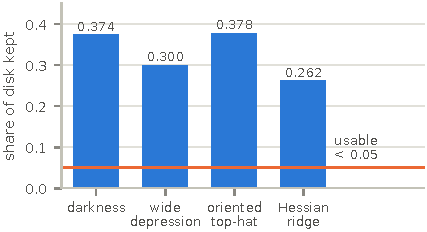
\includegraphics[width=0.62\textwidth]{figures/fig_classical.pdf}
\caption{The fraction of the solar disk that each classical quantity keeps when its threshold keeps
80\% of the filament pixels, averaged over three photographs. A usable proposal stage needs a value
well below 0.05. \generatedby{book/make\_book\_figures.py:fig\_classical}}
\label{fig:recall-classical}
\end{figure}

These tests apply each quantity \emph{globally}, over the whole disk. They do not test local evidence
of a ridge sampled in a narrow corridor ahead of the end of a detected filament, at the filament's own
width. That local use remains untested, and the global results should not be quoted against it. A
related test, exp076, used darkness, the coverage of dark pixels and elongation to rescue the
detector's weak proposals, rather than to propose new ones. Its best rule raised the number of true
positives from 860 to 882, but also raised the false positives from 397 to 446, and it lost (0.4546
against 0.4559).

\section{Semantic evidence}\label{sec:recall-semantic}
The dense models of Chapter~\ref{ch:paradigms} had lost as instance segmenters, but a semantic
probability map is independent evidence about where filaments are. We tried to use it in both
directions, to add masks and to remove them.

\paragraph{Adding masks.} In exp081 we used the frozen U-Net of exp004 to support weak proposals. A
proposal with a confidence between 0.26 and the floor was admitted when the semantic model's mean
probability inside it was at least 0.80. The validation score rose from 0.4559 to 0.4594, with true
positives rising from 860 to 891 and false positives from 397 to 438. Submitted as exp082, with 77
extra masks, it appeared on the leaderboard as 0.38, below the 0.39 of the same pipeline without them.
Two earlier probes that added masks with low confidence or small area (exp064 and exp065) had also
appeared as 0.38. The leaderboard consistently penalised additions that validation favoured by a few
thousandths.

\paragraph{Removing masks.} In exp085 we trained a new semantic model, based on a recent paper on
solar filaments by \citet{hu2026morden}. It used $5\times5$ convolutions, instance
normalisation~\citep{ulyanov2016}, parallel branches at several scales, channel gates in the manner
of squeeze-and-excitation~\citep{hu2018senet}, pooled context at several scales as in
PSPNet~\citep{zhao2017pspnet}, three input channels (the
raw image, a CLAHE version and a map of local dark contrast), a second output for the spine, and a
loss combining the focal loss~\citep{focal} with the Dice loss~\citep{vnet}. It trained in 25 minutes and reached a
Dice coefficient of 0.70 on masks and 0.64 on spines; on its own it scored a PQ of 0.3227. As evidence
for \emph{pruning}, however, it helped. In exp090 we removed a YOLO mask when the 75th percentile of
the semantic model's probability inside it was low, with a stricter bar near the centre of the disk
(0.30 within 0.65 of the radius) than near the limb (0.12). The validation score rose to 0.4606, and
the removals were correct 68\% of the time. In 500 bootstrap resamples the pruned rule beat the
baseline 93 to 95\% of the time, and on the leaderboard it appeared as 0.39, equal to our best score
at that time.

\section{What the recall work established}\label{sec:recall-summary}
The pool of candidates held most of the missing filaments, and an oracle showed that re-admitting the
right ones was worth about two hundredths. None of the verifiers that we built could pick them out
with the precision that the metric demands. Hand-made features, a crop classifier with the correct
labels, the opinion of a second architecture, physical contrast and a semantic model all fell short,
most of them far short. These measurements do not show that the task is impossible. They show that
the evidence available to these verifiers, in crops and features of the kinds we used, does not
separate a faint real filament from the surrounding network well enough. Our next step was therefore
to look for a detector whose candidates would need less rescuing.

\section*{Exercises}
\begin{exercise}{The emission rule}
Show that admitting one candidate that matches with probability $p$, with an expected IoU of $q$ when
it matches, raises PQ in expectation if and only if $pq > \tfrac12\PQ$. Relate this condition to
Equation~\eqref{eq:metric-breakeven}.
\end{exercise}

\begin{exercise}{The precision needed}
Using the table of blind floors in Section~\ref{sec:recall-arith}, compute the mean IoU $q$ of the 32
true positives added at a floor of 0.30, assuming that the numerator of PQ rose by exactly their IoUs.
Then check whether their precision of 0.25 should have raised or lowered PQ.
\end{exercise}

\begin{exercise}{Labels per record}
Write the labelling function for the verifier of exp134: given a photograph's records and one
proposal, return one label per record. How many training examples does a photograph with three
records and twenty proposals produce, and how should they be weighted so that heavily annotated
photographs do not dominate?
\end{exercise}

\begin{exercise}{A Hessian on a synthetic ridge}
Draw a dark Gaussian ridge of width $w$ on a bright background, and compute the eigenvalues of
$\mathbf{H}_\sigma$ at its centre for several values of $\sigma$. Show that the response peaks near
$\sigma \approx w$, and explain why a network of dark cells 5 to 15 pixels across also responds.
\end{exercise}

\begin{exercise}{Adding versus removing}
The rule of exp082 added 77 masks and appeared lower on the leaderboard, whereas the rule of exp090
removed masks and appeared equal. Suppose that the 90 photographs of the public leaderboard are an
independent sample, like the validation photographs. Estimate the standard deviation of the change in
the public score caused by 77 additions with a precision of 0.4, and decide whether the observed drop
is surprising.
\end{exercise}

\chapter{Transformers for Segmentation: From DETR to Mask2Former}\label{ch:transformers}

\section{Introduction}\label{sec:tr-intro}
In this chapter we build up the architecture of the final model one idea at a time. We assume that
the reader knows convolutional networks, but not that they remember the details of transformers, so
we start from the attention operation itself (Section~\ref{sec:tr-attention}). We then describe how
vision transformers, and in particular the Swin Transformer, adapt attention to images
(Section~\ref{sec:tr-swin}). Section~\ref{sec:tr-detr} introduces DETR, which treats detection as the
prediction of a set, and Section~\ref{sec:tr-maskformer} introduces MaskFormer, which extends this
idea from boxes to masks. Section~\ref{sec:tr-m2f} describes Mask2Former, the model we used, in
detail, including its loss and the way its outputs are turned into scored masks. Finally,
Section~\ref{sec:tr-why} explains why this architecture suits filaments.

\section{Attention}\label{sec:tr-attention}
A transformer operates on a \emph{set} of $n$ vectors called \keyterm{tokens},
$\mathbf{x}_1,\dots,\mathbf{x}_n\in\R^d$. In an image model, a token usually stands for a small patch
of pixels. The central operation, \keyterm{attention}~\citep{attention}, lets every token gather information from every
other token, weighted by how relevant each one is. Each token is projected in three ways by learned
matrices:
\begin{equation}
\mathbf{q}_i = W_Q\mathbf{x}_i, \qquad \mathbf{k}_j = W_K\mathbf{x}_j, \qquad \mathbf{v}_j = W_V\mathbf{x}_j .
\end{equation}
The \keyterm{query} $\mathbf{q}_i$ describes what token $i$ is looking for, the \keyterm{key}
$\mathbf{k}_j$ describes what token $j$ offers, and the \keyterm{value} $\mathbf{v}_j$ is what token
$j$ passes on if it is chosen. The output for token $i$ is a weighted mean of all the values, with
weights given by a softmax over the similarities between its query and every key:
\begin{equation}
\mathbf{y}_i = \sum_{j=1}^{n} a_{ij}\,\mathbf{v}_j, \qquad
a_{ij} = \frac{\exp(\mathbf{q}_i^{\top}\mathbf{k}_j/\sqrt{d_k})}{\sum_{j'}\exp(\mathbf{q}_i^{\top}\mathbf{k}_{j'}/\sqrt{d_k})}.
\end{equation}
Stacking the vectors as the rows of matrices gives the familiar form
\begin{equation}
\operatorname{Attention}(Q,K,V) = \softmax\!\Big(\frac{QK^{\top}}{\sqrt{d_k}}\Big)V,
\label{eq:tr-attention}
\end{equation}
where the softmax is taken along each row (Figure~\ref{fig:tr-attention}). The factor $1/\sqrt{d_k}$
matters. If the components of $\mathbf{q}$ and $\mathbf{k}$ are independent with unit variance, their
dot product has variance $d_k$, and without the scaling, large dot products would push the softmax
into saturation, where its gradients vanish (Exercise~\ref{ex:tr-sqrt}).

\begin{figure}[t]
\centering
\begin{tikzpicture}[
  tok/.style={circle, draw=vizblue!80!black, fill=vizblue!15, minimum size=0.42cm, inner sep=0pt,
              font=\sffamily\scriptsize},
  wcell/.style={minimum size=0.42cm, inner sep=0pt, draw=white, line width=0.5pt}]
  \foreach \i in {1,...,5} \node[tok] (x\i) at (0,-\i*0.5) {$x_{\i}$};
  \foreach \row [count=\rw] in {{55,20,10,10,5},{15,50,20,10,5},{5,15,45,25,10},{5,10,25,45,15},{5,5,10,20,60}}{
    \foreach \wt [count=\col] in \row {
      \pgfmathtruncatemacro{\shade}{min(100,\wt*1.6)}
      \node[wcell, fill=vizblue!\shade!white] at (1.5+\col*0.42, -\rw*0.5) {};
    }
  }
  \foreach \i in {1,...,5} \node[tok, draw=vizorange!80!black, fill=vizorange!15] (y\i) at (5.0,-\i*0.5) {$y_{\i}$};
  \draw[flow] (0.35,-1.5) -- (1.62,-1.5);
  \draw[flow] (3.95,-1.5) -- (4.6,-1.5);
  \node[note] at (2.76,-0.02) {keys $j$ (who is asked)};
  \node[note, anchor=west, text width=4.4cm, align=left] at (5.6,-1.5)
       {row $i$: weights $a_{ij}$, summing to one; output $y_i=\sum_j a_{ij}v_j$};
  \node[note] at (2.76,-3.05) {query $i$ asks each key; darker means more weight};
\end{tikzpicture}
\caption{Self-attention on five tokens. Each row of the weight matrix is one token's softmax over all
the tokens, and its output is the corresponding weighted mean of their values.
\drawnin{book/chapters/ch11\_transformers.tex}}
\label{fig:tr-attention}
\end{figure}

Listing~\ref{lst:tr-attention} implements Equation~\eqref{eq:tr-attention} in a few lines, with an
optional mask of forbidden pairs that we will need in Section~\ref{sec:tr-masked}.

\begin{lstlisting}[caption={Scaled dot-product attention with an optional mask.},label=lst:tr-attention]
def attention(q, k, v, forbidden=None):         # q: (n, d); k and v: (m, d)
    scores = q @ k.T / math.sqrt(q.shape[-1])   # (n, m): how much each query wants each key
    if forbidden is not None:                   # boolean (n, m): pairs that may not attend
        scores = scores.masked_fill(forbidden, float("-inf"))   # exp(-inf) = 0 weight
    return scores.softmax(dim=-1) @ v           # each output: a weighted mean of the values
\end{lstlisting}

Three refinements complete the basic picture. First, \keyterm{multi-head attention} runs $h$
attention operations in parallel, on separate projections of dimension $d/h$, and concatenates the
results, so that different heads can attend to different things. Second, in \keyterm{self-attention}
the queries, keys and values all come from the same set of tokens, whereas in
\keyterm{cross-attention} the queries come from one set and the keys and values from another.
Mask2Former uses both: its object queries attend to each other, and they attend to the image.
Third, a transformer layer wraps attention and a small two-layer perceptron (MLP) in residual
connections and normalisation, computing $\mathbf{y} = \mathbf{x} + \operatorname{Attn}(\mathbf{x})$
and then $\mathbf{z} = \mathbf{y} + \operatorname{MLP}(\mathbf{y})$, with a layer
normalisation~\citep{ba2016} before or after each step.

\subsection{The cost of attention, and where positions come from}\label{sec:tr-positions}
The matrix $QK^{\top}$ has $n^2$ entries, so the time and memory that attention needs grow with the
\emph{square} of the number of tokens. A $2048\times2048$ photograph at stride 4 has $512^2 = 262{,}144$
tokens, and a full attention matrix over them would have about $7\times10^{10}$ entries. This single
fact shapes every design in the rest of the chapter.

Attention is also blind to the order of the tokens: permuting the tokens permutes the outputs and
changes nothing else. Information about position must therefore be added explicitly. The DETR family
of models~\citep{detr} adds a fixed \keyterm{sine positional embedding}, adapted from the original
transformer~\citep{attention}. For a feature map of width $W$ and a
column $j$, the normalised position is $\tilde x = 2\pi\,(j+\tfrac12)/W$, and the embedding
interleaves
\begin{equation}
\mathrm{PE}_{2i}(\tilde x) = \sin\!\big(\tilde x / T^{2i/D}\big), \qquad
\mathrm{PE}_{2i+1}(\tilde x) = \cos\!\big(\tilde x / T^{2i/D}\big), \qquad T = 10{,}000,
\label{eq:tr-sine}
\end{equation}
for $i=0,1,\dots,D/2-1$, with the same construction for the rows. Note the normalisation by $W$.
Positions are expressed as fractions of the extent of the input, so two pixels a fixed distance apart
receive embeddings that differ \emph{less} in a large input than in a small one.
Section~\ref{sec:train-sampling} shows why this detail forced us to train the final model on whole
photographs as well as on crops.

\section{Vision transformers and Swin}\label{sec:tr-swin}
The \keyterm{Vision Transformer} (ViT)~\citep{vit} cuts an image into patches of $16\times16$ pixels,
embeds each patch as a token, and applies global self-attention. At $224\times224$ pixels this gives
only 196 tokens, and ViT classifies images well. For segmentation at the native resolution of our
photographs, however, it fails on both of the counts above: the number of tokens explodes, and a
single feature map at stride 16 is far too coarse for a filament four pixels wide.

The \keyterm{Swin Transformer}~\citep{swin} makes attention local and hierarchical, like a
convolutional network. It does so with five ideas.
\begin{itemize}[leftmargin=*,itemsep=2pt]
\item \textbf{Small patches.} The tokens are patches of $4\times4$ pixels, so the first feature map
has stride 4.
\item \textbf{Windows.} Self-attention runs only within non-overlapping windows of $M\times M$ tokens,
with $M=7$. For a map of $h\times w$ tokens with $C$ channels, this reduces the cost of a layer from
$4hwC^2 + 2(hw)^2C$ for global attention to
\begin{equation}
\Omega_{\text{window}} = 4hwC^2 + 2M^2hwC,
\end{equation}
which is linear in the number of tokens.
\item \textbf{Shifted windows.} Alternate layers shift the grid of windows by $\lfloor M/2\rfloor$
tokens (Figure~\ref{fig:tr-swin}), so that information crosses the borders of the windows from one
layer to the next.
\item \textbf{Merging.} Between stages, each $2\times2$ group of tokens is concatenated and projected
to a single token, which halves the resolution and doubles the number of channels. The four stages
therefore produce feature maps at strides 4, 8, 16 and 32, which is the pyramid that a segmentation
head needs.
\item \textbf{Relative position.} Inside a window, a learned bias $B$ that depends only on the offset
between two tokens is added to the attention scores~\citep{shaw2018}, giving $\softmax(QK^{\top}/\sqrt{d_k} + B)\,V$.
\end{itemize}

\begin{figure}[t]
\centering
\begin{tikzpicture}[scale=0.34]
  % regular windows: 2 x 2 windows of 4 x 4 patches
  \fill[vizblue!18] (0,4) rectangle (4,8); \fill[vizorange!18] (4,4) rectangle (8,8);
  \fill[vizaqua!18] (0,0) rectangle (4,4); \fill[vizyellow!22] (4,0) rectangle (8,4);
  \draw[gridline, line width=0.3pt] (0,0) grid (8,8);
  \draw[inkprimary, line width=0.9pt] (0,0) rectangle (8,8) (4,0) -- (4,8) (0,4) -- (8,4);
  % shifted windows: borders at 2 and 6
  \begin{scope}[shift={(12,0)}]
    \fill[vizblue!18] (2,2) rectangle (6,6);
    \fill[vizorange!18] (6,2) rectangle (8,6); \fill[vizorange!18] (0,2) rectangle (2,6);
    \fill[vizaqua!18] (2,6) rectangle (6,8); \fill[vizaqua!18] (2,0) rectangle (6,2);
    \fill[vizyellow!22] (0,0) rectangle (2,2); \fill[vizyellow!22] (6,6) rectangle (8,8);
    \fill[vizyellow!22] (0,6) rectangle (2,8); \fill[vizyellow!22] (6,0) rectangle (8,2);
    \draw[gridline, line width=0.3pt] (0,0) grid (8,8);
    \draw[inkprimary, line width=0.9pt] (0,0) rectangle (8,8) (2,0) -- (2,8) (6,0) -- (6,8)
         (0,2) -- (8,2) (0,6) -- (8,6);
  \end{scope}
  \node[note] at (4,-1.6) {layer $\ell$: regular windows};
  \node[note] at (16,-1.6) {layer $\ell+1$: shifted by half a window};
\end{tikzpicture}
\caption{Swin's shifted windows on an $8\times8$ map of tokens, with windows of $4\times4$ tokens.
Attention runs only inside each window with a thick border. In the next layer the grid is shifted, so
tokens that were separated by a border now share a window. Pieces of the same colour on the right are
joined into one window by a cyclic shift of the map. \drawnin{book/chapters/ch11\_transformers.tex}}
\label{fig:tr-swin}
\end{figure}

The backbone of the final model is \keyterm{Swin-S} (``small''), which has 96 channels in its first
stage, 2, 2, 18 and 2 blocks in its four stages, with 3, 6, 12 and 24 attention heads respectively,
and windows of $7\times7$ tokens. It came pretrained as part of a complete Mask2Former that had been
trained on the COCO instance segmentation task.

\section{DETR: detection as set prediction}\label{sec:tr-detr}
Most detectors, including the YOLO models of Chapter~\ref{ch:yolo}, produce many overlapping
candidates for each object and remove the duplicates afterwards with non-maximum suppression, a
hand-designed step with its own threshold. \keyterm{DETR}~\citep{detr} removed this step by changing
the question that the network answers. Instead of asking ``is there an object at this location?'', it
asks for a \emph{set} of objects.

DETR maintains $N$ learned vectors called \keyterm{object queries}, typically $N=100$. A transformer
decoder lets the queries attend to each other, through self-attention, and to the image features,
through cross-attention. Each query then outputs a probability distribution over the $K$ classes plus
a special class $\varnothing$, meaning ``no object'', together with a box. The output is always a set
of exactly $N$ predictions, most of which should predict $\varnothing$.

\subsection{Training with a one-to-one matching}\label{sec:tr-matching}
To compute a loss, each annotated object must be paired with the prediction that is responsible for
it. DETR chooses the pairing that is cheapest overall. Let the $M$ annotated objects be padded with
$\varnothing$ to a list $y_1,\dots,y_N$, and let $\mathfrak{S}_N$ be the set of permutations of $N$
elements. The matching is
\begin{equation}
\hat\sigma = \argmin_{\sigma\in\mathfrak{S}_N}\; \sum_{i=1}^{N} \mathcal{L}_{\text{match}}\big(y_i,\, \hat y_{\sigma(i)}\big),
\label{eq:tr-matching}
\end{equation}
where the matching cost $\mathcal{L}_{\text{match}}$ rewards a prediction for giving the object's
class a high probability and for placing its box (or, in later models, its mask) well, and pairing a
prediction with $\varnothing$ costs nothing. The loss is then computed on the matched pairs. Each
matched prediction is trained towards its object, and every unmatched prediction is trained towards
$\varnothing$, with the weight of that class reduced (to 0.1) because it occurs so often.

This is why DETR needs no step that removes duplicates. If two queries both describe the same
filament, only one of them is matched to it. The other is matched to $\varnothing$, and at every step
of training it is pushed towards predicting ``no object''. Since the queries also attend to each
other, they learn to coordinate, so that there is one query per object. For filaments, which the
annotators often draw as long structures that touch or break, predicting each object once is what the
metric rewards (Section~\ref{sec:metric-matching}).

\subsection{The Hungarian algorithm}\label{sec:tr-hungarian}
Equation~\eqref{eq:tr-matching} is an instance of the \keyterm{assignment problem}, which the
Hungarian algorithm~\citep{kuhn,munkres1957} solves exactly in $O(N^3)$ time. A greedy rule, which
pairs the cheapest remaining pair first, is not good enough. Figure~\ref{fig:tr-hungarian} gives an
example with three queries and two filaments in which the greedy pairing costs twice as much as the
optimal one, and Listing~\ref{lst:tr-hungarian} solves the same example with
SciPy~\citep{virtanen2020}, whose solver implements the method described by \citet{crouse2016}.

\begin{figure}[t]
\centering
\begin{tikzpicture}[
  cc/.style={minimum width=1.2cm, minimum height=0.5cm, draw=gridline, line width=0.5pt,
             font=\sffamily\footnotesize, text=inksecondary}]
  \foreach \sx/\ttl in {0/{greedy: cheapest pair first}, 5.4/{optimal assignment}}{
    \node[title] at (\sx+1.6,0.9) {\ttl};
    \node[note] at (\sx+1.0,0.42) {filament 1};
    \node[note] at (\sx+2.2,0.42) {filament 2};
    \foreach \q in {1,2,3} \node[note, anchor=east] at (\sx+0.35,-\q*0.5+0.5) {query \q};
  }
  % greedy picks (q1,f1) then (q3,f2)
  \node[cc, fill=vizorange!35] at (1.0,0) {0.10};  \node[cc] at (2.2,0) {0.20};
  \node[cc] at (1.0,-0.5) {0.15};                  \node[cc] at (2.2,-0.5) {0.90};
  \node[cc] at (1.0,-1.0) {0.50};                  \node[cc, fill=vizorange!35] at (2.2,-1.0) {0.60};
  \node[note] at (1.6,-1.65) {total $0.10+0.60 = 0.70$};
  % optimal picks (q1,f2) and (q2,f1)
  \begin{scope}[xshift=5.4cm]
    \node[cc] at (1.0,0) {0.10};                     \node[cc, fill=vizblue!30] at (2.2,0) {0.20};
    \node[cc, fill=vizblue!30] at (1.0,-0.5) {0.15}; \node[cc] at (2.2,-0.5) {0.90};
    \node[cc] at (1.0,-1.0) {0.50};                  \node[cc] at (2.2,-1.0) {0.60};
    \node[note] at (1.6,-1.65) {total $0.20+0.15 = 0.35$};
  \end{scope}
  \node[note, anchor=west, text width=3.0cm, align=left] at (8.6,-0.5)
       {the unmatched query is trained towards ``no object''};
\end{tikzpicture}
\caption{A matching cost matrix for three queries and two filaments. Taking the cheapest pair first
commits query 1 to filament 1 and forces an expensive second pair. The Hungarian algorithm finds the
assignment with the lowest total cost. \drawnin{book/chapters/ch11\_transformers.tex}}
\label{fig:tr-hungarian}
\end{figure}

\begin{lstlisting}[caption={The optimal assignment of Figure~\ref{fig:tr-hungarian}, found with the
SciPy solver that the Hugging Face matcher uses.},label=lst:tr-hungarian]
from scipy.optimize import linear_sum_assignment

cost = np.array([[0.10, 0.20],      # query 1 against filaments 1 and 2
                 [0.15, 0.90],      # query 2
                 [0.50, 0.60]])     # query 3
queries, filaments = linear_sum_assignment(cost)   # queries [0, 1], filaments [1, 0]
print(cost[queries, filaments].sum())              # 0.35; query 3 is left for "no object"
\end{lstlisting}

DETR had two well-known weaknesses. It trained slowly, needing hundreds of epochs on COCO, and it
found small objects poorly, because its global attention could only afford coarse features at stride
32. Deformable attention, described in Section~\ref{sec:tr-deform}, fixed both problems, and
Mask2Former inherits the fix.

\section{MaskFormer: segmentation as mask classification}\label{sec:tr-maskformer}
MaskFormer~\citep{maskformer} replaced DETR's boxes with masks. A \keyterm{pixel decoder} upsamples
the backbone's features into a map of \keyterm{per-pixel embeddings}
$\mathbf{F}\in\R^{C\times\frac H4\times\frac W4}$. Each query, after the transformer decoder, produces
a class distribution $\mathbf{p}_q$ and a \keyterm{mask embedding} $\mathbf{e}_q\in\R^{C}$. Its mask
is the sigmoid of a dot product at every pixel,
\begin{equation}
m_q(\mathbf{u}) = \sigmoid\big(\mathbf{e}_q^{\top}\mathbf{F}(\mathbf{u})\big).
\label{eq:tr-mask}
\end{equation}
Compare this with Equation~\eqref{eq:yolo-mask}. In YOLO, 32 prototypes are
shared by all the detections in an image, and each detection mixes them with 32 coefficients. Here the
per-pixel embedding has 256 channels, and each query's mask embedding is computed \emph{by attending
to the image}, so every query can build a mask that is specific to its own object. The same model can
perform semantic, instance and panoptic segmentation; only the post-processing differs.

\section{Mask2Former}\label{sec:tr-m2f}
\keyterm{Mask2Former}~\citep{mask2former} is MaskFormer with four changes, which together made it the
strongest general-purpose segmentation model of its time: masked attention, deformable attention in
the pixel decoder, queries that attend to several scales in turn, and a loss computed on sampled
points. Figure~\ref{fig:tr-m2f} shows the whole model as we used it, and we describe the four changes
in turn.

\begin{figure}[t]
\centering
\begin{tikzpicture}[
  st/.style={box=#1, text width=1.9cm, minimum height=0.62cm, font=\sffamily\scriptsize,
             execute at begin node={\hyphenpenalty=10000}},
  big/.style={box=#1, font=\sffamily\scriptsize, execute at begin node={\hyphenpenalty=10000}}]
  \node[inner sep=0pt] (img) at (-1.75,0) {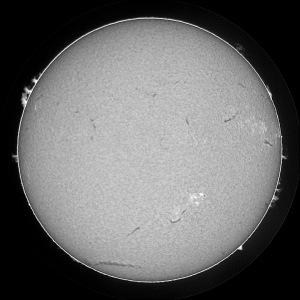
\includegraphics[width=1.0cm]{figures/thumb_input.png}};
  \node[note, below=2pt of img] {photograph};
  \node[st=vizblue] (s1) at (0.4,1.2) {Swin stage 1: 1/4};
  \node[st=vizblue] (s2) at (0.4,0.4) {Swin stage 2: 1/8};
  \node[st=vizblue] (s3) at (0.4,-0.4) {Swin stage 3: 1/16};
  \node[st=vizblue] (s4) at (0.4,-1.2) {Swin stage 4: 1/32};
  \draw[flow] (img.east) -- (s1.west |- 0,0);
  \node[big=vizaqua, text width=2.3cm, minimum height=3.0cm] (pd) at (3.35,0)
       {\textbf{\color{inkprimary}pixel decoder}\\[2pt] 6 layers of multi-scale deformable attention on 1/8, 1/16, 1/32; upsampled and fused to 1/4};
  \foreach \s in {s1,s2,s3,s4} \draw[flow] (\s.east) -- (\s.east -| pd.west);
  \node[big=vizorange, text width=2.55cm, minimum height=3.0cm] (dec) at (6.75,0)
       {\textbf{\color{inkprimary}transformer decoder}\\[2pt] 9 layers; each: masked cross-attention to one scale (1/32, 1/16, 1/8 in turn), self-attention among queries, MLP};
  \node[st=vizorange, text width=2.1cm] (q) at (6.75,2.2) {100 learned object queries};
  \draw[flow] (q) -- (dec);
  \draw[flow] (pd.east |- 0,0.6) -- (dec.west |- 0,0.6);
  \node[st=vizaqua] (F) at (3.35,-2.35) {per-pixel embeddings $\mathbf{F}$ at 1/4};
  \draw[flow] (pd) -- (F);
  \node[st=vizorange, text width=1.8cm] (cls) at (9.6,0.8) {class: filament or no object};
  \node[st=vizorange, text width=1.8cm] (emb) at (9.6,-0.4) {mask embedding $\mathbf{e}_q$};
  \node[st=inkmuted, text width=1.8cm] (mask) at (9.6,-2.35) {mask $\sigmoid(\mathbf{e}_q^{\top}\mathbf{F})$ at 1/4};
  \draw[flow] (dec.east |- cls) -- (cls);
  \draw[flow] (dec.east |- emb) -- (emb);
  \draw[flow] (emb) -- (mask);
  \draw[flow] (F) -- (mask);
  \draw[dashflow] (mask.north west) to[bend left=18] (dec.south east);
  \node[note] at (6.75,-1.93) {each layer's masks restrict\\ the next layer's attention};
\end{tikzpicture}
\caption{Mask2Former as used in this project. The Swin-S backbone produces four feature maps. The
pixel decoder refines the three coarsest with deformable attention and produces per-pixel embeddings
at a quarter of the input resolution. The 100 queries pass through nine decoder layers, each of which
attends only inside the query's current mask, and each query ends with a class and a mask.
\drawnin{book/chapters/ch11\_transformers.tex}}
\label{fig:tr-m2f}
\end{figure}

\subsection{Masked attention}\label{sec:tr-masked}
In MaskFormer, the cross-attention of each query looks at the whole image. Mask2Former restricts it to
the query's own object. Before each decoder layer $\ell$, the query's mask predicted by the previous
layer is thresholded at one half, and cross-attention is forbidden outside it. Let $X_\ell$ denote the
query features after layer $\ell$, let $Q_\ell = W_Q X_{\ell-1}$, and let $K_\ell$ and $V_\ell$ be
computed from the image features at the scale used by layer $\ell$. Then
\begin{equation}
X_\ell = \softmax\!\big(\mathcal{M}_{\ell-1} + Q_\ell K_\ell^{\top}\big)\,V_\ell + X_{\ell-1},
\label{eq:tr-masked}
\end{equation}
where the attention mask is
\begin{equation*}
\mathcal{M}_{\ell-1}(\mathbf{u}) =
\begin{cases} 0 & \text{if } m_q^{\ell-1}(\mathbf{u}) \ge 0.5,\\ -\infty & \text{otherwise.}\end{cases}
\end{equation*}
The entries equal to $-\infty$ receive zero weight after the softmax, just as the \texttt{forbidden}
argument of Listing~\ref{lst:tr-attention} does. If a query's mask is empty, the restriction is lifted
for that query, so that it can search the whole image. As a result, each query refines its object using
features from the object's own neighbourhood, instead of averaging over the whole photograph, and the
model converges much faster than MaskFormer.

\subsection{Deformable attention in the pixel decoder}\label{sec:tr-deform}
The pixel decoder must let every location of three large feature maps exchange information, which
full attention cannot afford. It therefore uses \keyterm{multi-scale deformable
attention}~\citep{deformabledetr}. Instead of attending to every key, each query attends to a small
number of \emph{sampled} points around a reference location, at every scale
(Figure~\ref{fig:tr-deform}). For a query with features $\mathbf{z}_q$ and a normalised reference point
$\hat{\mathbf{p}}_q\in[0,1]^2$, over the feature maps $\mathbf{x}^1,\dots,\mathbf{x}^L$, the output is
\begin{equation}
\operatorname{MSDeformAttn}(\mathbf{z}_q, \hat{\mathbf{p}}_q)
= \sum_{m=1}^{H} W_m \Big[\sum_{l=1}^{L}\sum_{k=1}^{K} A_{mlqk}\,
W'_m\,\mathbf{x}^{l}\big(\phi_l(\hat{\mathbf{p}}_q) + \Delta\mathbf{p}_{mlqk}\big)\Big],
\label{eq:tr-deform}
\end{equation}
where $m$ runs over $H=8$ heads, $l$ over $L=3$ scales and $k$ over $K=4$ sampled points. The function
$\phi_l$ converts the reference point into the pixel coordinates of level $l$. The offsets
$\Delta\mathbf{p}_{mlqk}$ and the weights $A_{mlqk}$ are predicted from $\mathbf{z}_q$ by linear layers,
and the weights are normalised by a softmax over the pairs $(l,k)$. The offsets are fractional, so the
feature map $\mathbf{x}^l(\cdot)$ is read by \keyterm{bilinear interpolation} of its four nearest
feature vectors.

Each query therefore touches only $H\cdot L\cdot K = 96$ sampled points instead of every location, so
the cost is linear in the number of pixels. The offsets are also learned, so the model decides where
to look. In the pixel decoder, every location of the three coarsest maps acts as a query, with
its own position as the reference point, and six such layers are stacked.

\begin{figure}[t]
\centering
\begin{tikzpicture}[
  sp/.style={circle, fill=vizorange, inner sep=0pt, minimum size=4pt},
  rp/.style={draw=inkprimary, line width=0.9pt, cross out, minimum size=5pt, inner sep=0pt}]
  \foreach \sx/\n/\lab in {0/8/{level 1: fine}, 2.9/4/{level 2}, 5.8/2/{level 3: coarse}}{
    \begin{scope}[xshift=\sx cm]
      \pgfmathsetmacro{\gstep}{2.2/\n}
      \fill[vizaqua!10] (0,0) rectangle (2.2,2.2);
      \draw[gridline, line width=0.4pt, step=\gstep cm] (0,0) grid (2.2,2.2);
      \draw[inkmuted, line width=0.6pt] (0,0) rectangle (2.2,2.2);
      \node[rp] at (1.2,1.0) {};
      \node[note] at (1.1,-0.3) {\lab};
    \end{scope}
  }
  \foreach \dx/\dy in {0.35/0.45, -0.4/0.25, 0.15/-0.45, 0.6/-0.1}
    { \node[sp] (p) at (1.2+\dx,1.0+\dy) {}; \draw[->, line width=0.5pt, draw=vizorange!80!black] (1.2,1.0) -- (p); }
  \foreach \dx/\dy in {0.55/0.6, -0.65/0.1, 0.3/-0.6, -0.2/0.75}
    { \node[sp] (p) at (4.1+\dx,1.0+\dy) {}; \draw[->, line width=0.5pt, draw=vizorange!80!black] (4.1,1.0) -- (p); }
  \foreach \dx/\dy in {0.7/0.8, -0.85/-0.3, 0.45/-0.75, -0.5/0.85}
    { \node[sp] (p) at (7.0+\dx,1.0+\dy) {}; \draw[->, line width=0.5pt, draw=vizorange!80!black] (7.0,1.0) -- (p); }
  \node[box=vizorange, text width=2.3cm, font=\sffamily\scriptsize] at (10.3,1.1)
       {weighted sum of the 12 sampled values ($A_{lk}$, softmax over levels and points)};
\end{tikzpicture}
\caption{Multi-scale deformable attention for one head. The same reference point (cross) is located
at every level. The query predicts four fractional offsets per level (dots) and a weight for each,
reads each value by bilinear interpolation, and returns their weighted sum.
\drawnin{book/chapters/ch11\_transformers.tex}}
\label{fig:tr-deform}
\end{figure}

\subsection{Multi-scale queries and deep supervision}\label{sec:tr-deep}
The transformer decoder has nine layers, and they use the scales produced by the pixel decoder in
turn: layer 1 attends to the map at stride 32, layer 2 to the map at stride 16, layer 3 to the map at
stride 8, and the cycle repeats three times. The coarse maps provide context cheaply, and the fine maps
provide detail. Each layer also performs cross-attention \emph{before} self-attention, so that the
queries look at the image before they coordinate with each other, and the initial features of the
queries are learned, whereas MaskFormer sets them to zero.

A prediction, consisting of a class and a mask for every query, is made from the initial queries and
again after each of the nine layers. All ten predictions are matched to the annotations and all ten
are penalised. This is called \keyterm{deep supervision}~\citep{lee2015dsn}: every layer is trained to produce a usable
answer, so the gradients reach the early layers directly.

\subsection{The loss, with point sampling}\label{sec:tr-loss}
For a matched pair of a query and an annotated filament, the loss has three terms: a cross-entropy on
the class, a per-pixel binary cross-entropy between the predicted and annotated masks, and a Dice loss
(Equation~\eqref{eq:par-dice}),
\begin{equation}
\mathcal{L} = \lambda_{\text{cls}}\mathcal{L}_{\text{cls}} + \lambda_{\text{mask}}\mathcal{L}_{\text{BCE}}
+ \lambda_{\text{dice}}\mathcal{L}_{\text{Dice}}, \qquad
(\lambda_{\text{cls}}, \lambda_{\text{mask}}, \lambda_{\text{dice}}) = (2, 5, 5),
\label{eq:tr-loss}
\end{equation}
with the ``no object'' class weighted by 0.1 in the cross-entropy. The mask and Dice terms are summed
over the matched pairs and divided by the number of annotated masks in the batch, and the class term is
normalised by the total class weight. The matching cost of Equation~\eqref{eq:tr-matching} uses the
same three terms.

Evaluating the mask terms at every pixel of a crop of 1024 pixels, for up to 100 queries and ten
predictions, would be very expensive. Mask2Former therefore evaluates them at a sample of $P = 12{,}544$
points per mask, chosen by \keyterm{importance sampling}~\citep{pointrend}. It draws $3P$ points
uniformly at random, keeps the $0.75P$ of them at which the prediction is most uncertain (those whose
logit is closest to zero, which lie along the predicted boundary), and adds $0.25P$ fresh uniformly
drawn points. The annotated mask is read at the same continuous coordinates by bilinear interpolation.
Two consequences of this scheme matter for us. First, the loss concentrates on boundaries, where
Chapter~\ref{ch:post} found most of the error. Second, because the annotated mask is sampled at
fractional positions of a target at the native resolution, the supervision is finer than the model's
output grid at stride 4.

\subsection{The configuration we used}\label{sec:tr-config}
We used version 4.57.6 of the Hugging Face \texttt{transformers} implementation~\citep{wolf2020} with the checkpoint
\texttt{facebook/\allowbreak mask2former-\allowbreak swin-\allowbreak small-\allowbreak coco-\allowbreak instance}.\footnote{Several details in this chapter, such
as the normalisation of the positional embeddings, were read from the source code of this pinned
version rather than from the paper, because the two can differ.} The model has about 69 million
parameters,
100 queries and a hidden size of 256, and we used its loss exactly as shipped. We re-initialised the
classification head for a single class. At most 26 filaments appear in any validation record, and at
most 23 in any training record, so 100 queries are never too few.

\subsection{From queries to scored masks}\label{sec:tr-inference}
At test time every query yields a candidate. Its class probability $p_q$ is the softmax probability of
``filament'' against ``no object''. Its mask logits are enlarged from a quarter of the resolution to
$2048\times2048$ by bilinear interpolation, and thresholded at zero, which corresponds to a probability
of one half. Its score multiplies the class probability by the mean mask probability inside the binary
mask,
\begin{equation}
s_q = p_q \cdot \frac{\sum_{\mathbf{u}} \sigmoid(m_q(\mathbf{u}))\,\mathbf{1}[m_q(\mathbf{u})>0]}
{\sum_{\mathbf{u}} \mathbf{1}[m_q(\mathbf{u})>0]} ,
\label{eq:tr-score}
\end{equation}
where $m_q(\mathbf{u})$ now denotes the upsampled mask logit. The second factor rewards confident
masks: a query that is sure that a filament exists but unsure of its extent receives a lower score.
Listing~\ref{lst:tr-predict} shows our implementation.

\begin{lstlisting}[caption={Candidates from one forward pass. Condensed from
\file{experiments/exp\_139\_mask2former/src/model.py:predict}.},label=lst:tr-predict]
@torch.inference_mode()
def predict(model, gray, device, floor=0.02, min_pixels=40, chunk=8):
    pixels = gpu_pixels(torch.from_numpy(gray)[None], None, device)   # grey -> 3 channels, normalised
    output = model(pixel_values=pixels)
    probability = output.class_queries_logits[0].float().softmax(-1)[:, 0]   # filament vs no object
    logits = output.masks_queries_logits[0]                                  # (100, H/4, W/4)
    keep = torch.nonzero(probability >= floor).flatten()
    candidates = []
    for start in range(0, len(keep), chunk):                                 # bounded memory
        queries = keep[start:start + chunk]
        upsampled = F.interpolate(logits[queries][None].float(), size=gray.shape,
                                  mode="bilinear", align_corners=False)[0]   # to 2048 x 2048
        binary = upsampled > 0
        area = binary.flatten(1).sum(1)
        inside = (upsampled.sigmoid() * binary).flatten(1).sum(1) / area.clamp(min=1)
        scores = probability[queries] * inside       # class probability x mean mask probability
        for j in range(len(queries)):
            if int(area[j]) >= min_pixels:
                candidates.append((float(scores[j]), binary[j].to(torch.uint8).cpu().numpy()))
    return candidates
\end{lstlisting}

The candidates then pass through the same emission rule that we used for every earlier model. We keep
the candidates whose score clears a threshold, paint them in order of decreasing score so that the
masks become disjoint (Section~\ref{sec:masks-paint}), and drop pieces smaller than a minimum area. For
the deployed model, the threshold was 0.85, with no erosion and a minimum area of 100 pixels
(Chapter~\ref{ch:submission}).

\section{Why this architecture suits filaments}\label{sec:tr-why}
Three properties connect Mask2Former to the lessons of the earlier chapters. We argue for each of
them here, and the following chapters measure them.
\begin{enumerate}[leftmargin=*,itemsep=2pt]
\item \textbf{Each filament is predicted once.} The one-to-one matching trains the model to describe
every object once, without a step that suppresses duplicates. The YOLO pipeline needed non-maximum
suppression and, at its best, fusion over eight views, whereas a single view of the Mask2Former beat
every fused YOLO pipeline.
\item \textbf{Each mask is built from the image, for its own object.} A YOLO mask mixes 32 prototypes
that are shared by the whole photograph. A Mask2Former mask comes from a 256-dimensional embedding that
its query computed by attending, through masked attention, to the neighbourhood of its own object.
\item \textbf{The masks lie on a grid of stride 4 in native pixels.} The masks are predicted at a
quarter of the input resolution, so if the input is the native photograph, the mask grid has cells
four native pixels wide. Section~\ref{sec:train-resolution} shows that a perfect mask on this grid
could still reach a mean IoU of 0.914 with the annotations, whereas a grid with cells eight native
pixels wide is limited to 0.771.
\end{enumerate}
The price is memory and engineering effort. The model is large, its attention is irregular, and
training it at the native resolution on thousands of crops required the careful work described in
Chapter~\ref{ch:training}.

\section*{Exercises}
\begin{exercise}{Why divide by $\sqrt{d_k}$?}\label{ex:tr-sqrt}
Let $\mathbf{q},\mathbf{k}\in\R^{d}$ have independent components with mean 0 and variance 1. Show that
$\mathbf{q}^{\top}\mathbf{k}$ has variance $d$. What happens to the softmax of $n$ such scores as $d$
grows, if the scores are not scaled?
\end{exercise}

\begin{exercise}{The cost of windows}
For a crop of $1024\times1024$ pixels, compute the number of tokens at stride 4, and the number of
attention scores per layer with global attention and with windows of $7\times7$ tokens. How much memory
would the global matrix of scores need in 16-bit floating point?
\end{exercise}

\begin{exercise}{The sine embedding across extents}
Using Equation~\eqref{eq:tr-sine}, compute the difference between the embeddings of two pixels 16
native pixels apart, in a crop of 1024 pixels and in a frame of 2048 pixels, for the lowest and the
highest frequencies. Explain why a model trained only on crops sees an unfamiliar pattern of positions
at 2048 pixels.
\end{exercise}

\begin{exercise}{Greedy versus Hungarian}
Construct a $3\times3$ cost matrix on which greedy matching costs more than three times as much as the
optimal matching. Can the greedy matching ever be worse than the optimal one when every row and every
column has a single, clearly cheapest entry?
\end{exercise}

\begin{exercise}{Point sampling}
Implement importance sampling for one predicted mask: draw $3P$ uniform points, keep the $0.75P$ most
uncertain ones, and add $0.25P$ uniform points. On a real filament mask and a slightly shifted
prediction of it, compare the Dice loss computed on the sampled points with the Dice loss computed on
all pixels, for $P$ between 100 and 12,544.
\end{exercise}

\chapter{Training the Final Model}\label{ch:training}

\section{Introduction}\label{sec:train-first}
\epigraph{We should forget about small efficiencies, say about 97\% of the time: premature
optimization is the root of all evil.}{Donald Knuth, \emph{Structured Programming with go to
Statements} \citeyearpar{knuth1974}}

Our first Mask2Former, exp046, was trained on a Kaggle TPU. It shrank every photograph from 2048 to
1024 pixels, used the smaller Swin-T backbone and our own re-implementation of the Hungarian loss, and
ran with a batch size of 1 in 16-bit arithmetic with activation checkpointing. The session limit
stopped it after 2,309 steps, and it scored 0.300 on validation. A continuation (exp058) trained for
about 1,600 more steps, bringing the total to about four epochs of the fifty that had been planned,
and its score fell to 0.247. Submitted as a probe, it appeared on the leaderboard as 0.20. Fused with
the eight-view predictions of the YOLO models (exp048), it also lowered their score, from 0.4571 to
0.4472.

It would have been easy to conclude from this that Mask2Former does not suit filaments. Our
pre-registration (Section~\ref{sec:val-oracles}) explicitly rejected that conclusion, recording that
the architecture had not yet been tested. The model had been stopped a tenth of the way through its
schedule, it had seen the photographs at half their resolution, and its loss was new code that had
never been checked against a reference implementation. None of these results measures the
architecture itself.

This chapter describes the run that did test it, and each of its design choices answers one of the
faults of the first attempt. Section~\ref{sec:train-resolution} measures the cost of resolution and
explains why we never shrink the photograph. Section~\ref{sec:train-sampling} describes how the
training samples are drawn, and Section~\ref{sec:train-optim} the optimiser and its schedule.
Sections~\ref{sec:train-memory}--\ref{sec:train-accumulation} cover memory, speed and a subtle
problem with gradient accumulation, and Section~\ref{sec:train-run} describes the training run
itself.

\section{Resolution: what a mask grid can represent}\label{sec:train-resolution}
Mask2Former predicts masks at a quarter of the size of its input. Since exp046 fed it images of 1024
pixels, its masks lay on a grid of $256\times256$ cells, with one cell for every $8\times8$ native
pixels. Before training again, we measured what this costs (exp136). We took every annotated mask,
averaged it down onto a coarse grid, enlarged it back bilinearly, and thresholded it at one half. The
result is the best that a \emph{perfect} mask head on that grid could produce:
\begin{center}\small
\begin{tabular}{@{}lccc@{}}
\toprule
cell size (native pixels) & mean IoU & thin filaments ($\le3$ px) & IoU above 0.5 \\
\midrule
2 (a 1024 grid) & 0.976 & 0.971 & 100\% \\
\textbf{4 (a 512 grid)} & \textbf{0.914} & \textbf{0.896} & \textbf{99.9\%} \\
8 (a 256 grid) & 0.771 & 0.713 & 95.8\% \\
\bottomrule
\end{tabular}
\end{center}
On a grid with cells of 8 pixels, even a perfect model loses almost a quarter of the IoU on every
filament, and more on thin ones. With cells of 4 pixels, the loss is less than a tenth.
Figure~\ref{fig:train-grid} shows why: a body four pixels wide can be traced by cells four pixels wide,
but not by cells eight pixels wide.

\begin{figure}[t]
\centering
\begin{tikzpicture}
  % (a) 4-pixel cells
  \begin{scope}
    \foreach \cx/\cy in {0/1, 1/1, 2/2, 3/2, 4/3, 5/3, 6/4, 7/4}
      \fill[vizblue!35] (\cx*0.4,\cy*0.4) rectangle ++(0.4,0.4);
    \begin{scope}
      \clip (0,0) rectangle (3.2,2.0);
      \draw[vizorange, line width=0.4cm, opacity=0.55] (-0.2,0.3) -- (3.4,2.1);
    \end{scope}
    \draw[gridline!70!black, line width=0.3pt, step=0.4] (0,0) grid (3.2,2.0);
    \draw[inkmuted, line width=0.6pt] (0,0) rectangle (3.2,2.0);
    \node[note] at (1.6,-0.35) {(a) cells of 4 native pixels};
  \end{scope}
  % (b) 8-pixel cells
  \begin{scope}[xshift=4.6cm]
    \foreach \cx/\cy in {0/0, 1/1, 2/1, 3/2}
      \fill[vizblue!35] (\cx*0.8,\cy*0.8) rectangle ++(0.8,0.8);
    \begin{scope}
      \clip (0,0) rectangle (3.2,2.4);
      \draw[vizorange, line width=0.4cm, opacity=0.55] (-0.2,0.3) -- (3.4,2.1);
    \end{scope}
    \draw[gridline!70!black, line width=0.3pt, step=0.8] (0,0) grid (3.2,2.4);
    \draw[inkmuted, line width=0.6pt] (0,0) rectangle (3.2,2.4);
    \node[note] at (1.6,-0.35) {(b) cells of 8 native pixels};
  \end{scope}
  \fill[vizorange, opacity=0.55] (8.7,1.6) rectangle (9.1,1.8);
  \node[note, anchor=west] at (9.2,1.7) {filament, 4 px wide};
  \fill[vizblue!35] (8.7,1.1) rectangle (9.1,1.3);
  \node[note, anchor=west] at (9.2,1.2) {cells more than\\ half covered};
\end{tikzpicture}
\caption{A filament four pixels wide on two mask grids. With cells of 4 pixels (a), the cells that are
more than half covered trace the body closely. With cells of 8 pixels (b), the best binary trace is a
coarse staircase. The measured ceilings in the table use a smoother encoding than this binary one, but
the ordering is the same. \drawnin{book/chapters/ch12\_training.tex}}
\label{fig:train-grid}
\end{figure}

A second measurement (exp138) put these numbers in context. Scoring one annotator's masks against
another's gave a mean IoU of 0.576, with 74\% of the filaments that both annotators drew above an IoU
of 0.5. Encoding the first annotator's masks on a grid with cells of 4 pixels changed this agreement
by only 0.013. Below cells of 4 pixels, then, any gain in precision is swamped by the differences in
how people draw. Our notes first called this a ``bound'' on the quality of the boundaries, and later
corrected themselves: it measures the agreement between people, and it does not limit what a model
can score against any one of them (Section~\ref{sec:metric-agreement}).

The decision followed directly: \emph{we never shrink the photograph}. Every pixel the model sees is
a native pixel, so its masks come out on the grid with cells of 4 pixels. Two further details keep the
supervision at least that fine. The annotations are rasterised with \texttt{pycocotools} at the native
resolution, using the scorer's own convention (Section~\ref{sec:masks-raster}), and the loss reads
them at fractional point coordinates (Section~\ref{sec:tr-loss}), so the targets are never quantised
to the output grid.

\section{Crops and whole frames}\label{sec:train-sampling}
A batch of eight native $2048\times2048$ frames does not fit on any single GPU that we could rent at a
sensible price, and most of a frame is empty disk anyway. Training therefore uses \keyterm{crops}:
windows of $1024\times1024$ pixels centred on a randomly chosen annotated filament, with the centre
moved at random by up to 35\% of the crop, so that filaments do not always sit in the middle. Since 99\%
of the filaments in the training set are shorter than 516 pixels, a crop almost always contains its
anchor filament whole, and it usually contains several of its neighbours too.

Crops alone, however, would have caused a subtle failure. Section~\ref{sec:tr-positions} noted that the
sine positional embeddings of Equation~\eqref{eq:tr-sine} are normalised by the size of the input. A
model that had only ever seen inputs of 1024 pixels would meet, at test time on a frame of 2048 pixels,
embeddings that change half as fast per pixel as anything it saw during training. We therefore use
\keyterm{whole frames} for a quarter of all optimiser steps, keeping the number of pixels per step
constant: a step processes either eight crops of 1024 pixels or two whole frames of 2048 pixels
(Figure~\ref{fig:train-sampling}). Whole frames also contain every kind of negative example on the
disk, such as the dark network and the limb, far from any filament.

\begin{figure}[t]
\centering
\begin{tikzpicture}
  % a frame with a crop centred on a filament
  \fill[gridline!55] (0,0) rectangle (2.6,2.6);
  \draw[inkmuted, line width=0.6pt] (0,0) rectangle (2.6,2.6);
  \draw[inkprimary!70, line width=2.2pt, line cap=round] (0.95,1.35) .. controls (1.2,1.6) and (1.5,1.55) .. (1.75,1.3);
  \draw[inkprimary!55, line width=1.6pt, line cap=round] (0.4,0.5) .. controls (0.6,0.7) and (0.9,0.7) .. (1.1,0.6);
  \draw[vizblue, line width=1.0pt, dashed] (0.72,0.88) rectangle (2.02,2.18);
  \node[note] at (1.3,-0.35) {2048 frame; a 1024 crop};
  \node[note] at (1.3,-0.72) {around a random filament};
  % steps
  \node[title, anchor=west] at (3.4,2.45) {75\% of optimiser steps: 8 crops of 1024};
  \foreach \i in {0,...,7} \fill[vizblue!45] (3.45+\i*0.62,1.55) rectangle ++(0.5,0.5);
  \node[title, anchor=west] at (3.4,1.05) {25\% of steps: 2 whole frames of 2048};
  \foreach \i in {0,1} \fill[vizorange!45] (3.45+\i*1.15,-0.1) rectangle ++(1.0,1.0);
  \node[note, anchor=west, text width=3.3cm, align=left] at (6.0,0.4)
       {equal pixels per step: $8\times1024^2 = 2\times2048^2$};
\end{tikzpicture}
\caption{How training samples are drawn. Most steps use crops centred on a randomly chosen annotated
filament (dashed), and a quarter of the steps use whole native frames, so that the model also sees
full-size positional embeddings and the whole disk. \drawnin{book/chapters/ch12\_training.tex}}
\label{fig:train-sampling}
\end{figure}

Every annotation \emph{record} is its own sample, so a photograph labelled by three people appears
three times, each time with one person's masks, because the metric scores each record against one
annotator (Section~\ref{sec:data-records}). The sampler sizes an epoch as two crops per training
record, which gives $\lfloor 974\times2/8\rfloor = 243$ steps per epoch, a quarter of them with whole
frames, so 50 epochs amount to 12,150 steps. Records are drawn in shuffled rounds, so that every record
appears once before any record repeats. Listing~\ref{lst:train-sampler} shows how the sampler plans
the steps of an epoch.

\begin{lstlisting}[caption={Planning optimiser steps of crops or whole frames. Condensed from
\file{experiments/exp\_139\_mask2former/src/data.py:ExtentBatchSampler}.},label=lst:train-sampler]
def __iter__(self):
    rng = np.random.default_rng([self.seed, self.epoch, 7])      # a new plan every epoch
    kinds = np.array([True] * self.whole_steps + [False] * (self.steps - self.whole_steps))
    rng.shuffle(kinds)                                           # which steps are whole frames
    stream = []
    for whole in kinds:
        size = self.whole_batch if whole else self.batch         # 2 frames or 8 crops
        while len(stream) < size:
            stream.extend(rng.permutation(self.records).tolist())   # every record, in turn
        chosen, stream = stream[:size], stream[size:]
        extent = 2048 if whole else self.crop
        # the epoch travels inside each index: persistent workers never see set_epoch()
        yield [(record, extent, self.epoch, slot) for slot, record in enumerate(chosen)]
\end{lstlisting}

The comment on the last line of the listing records a bug that we caught before the run. With
persistent data-loader workers, each worker process holds its own copy of the dataset object, and a
call to \texttt{set\_epoch} in the main process never reaches that copy. Every epoch would then have
repeated the crops of the first epoch. Passing the epoch inside every sample index fixed the problem.

\subsection{Augmentation}\label{sec:train-augmentation}
Each sample is flipped horizontally and vertically at random, and turned by a random multiple of
$90^\circ$. These transformations form the dihedral group of Section~\ref{sec:tta-d4}, and they are
exact on the pixel grid. Is this physically safe? The Sun's filaments are not oriented at random
everywhere. Among the 4,894 elongated training filaments (those whose length is at least three times
their width), the orientation is isotropic near the equator: within 0.3 of the solar radius above or
below the centre of the disk, 50\% lie closer to east--west than to north--south. The share rises to
60.5\% between 0.3 and 0.6 radii from the equator, and to 88\% beyond 0.6 radii. Only 3.8\% of the filaments lie in this last band,
however. The turns therefore misplace a latitude-dependent tendency for a few percent of the
filaments, and in exchange every view that test-time augmentation might show the model remains within
the training distribution. We vary the brightness only mildly, with a gamma between 0.8 and 1.25 and a
gain between 0.85 and 1.15.

\section{Optimisation}\label{sec:train-optim}
The optimiser is \keyterm{AdamW}~\citep{adamw}, as in the Mask2Former paper. For a parameter $\theta$
with gradient $g_t$ at step $t$, Adam~\citep{kingma2015} keeps running averages of the gradient and of its square,
\begin{equation}
m_t = \beta_1 m_{t-1} + (1-\beta_1)\,g_t, \qquad v_t = \beta_2 v_{t-1} + (1-\beta_2)\,g_t^2,
\end{equation}
corrects the bias that these averages have at the start of training, $\hat m_t = m_t/(1-\beta_1^t)$ and
$\hat v_t = v_t/(1-\beta_2^t)$, and updates the parameter as
\begin{equation}
\theta_t = \theta_{t-1} - \eta_t\Big(\frac{\hat m_t}{\sqrt{\hat v_t}+\epsilon} + \lambda\,\theta_{t-1}\Big),
\qquad \beta_1 = 0.9,\ \beta_2 = 0.999 .
\label{eq:train-adamw}
\end{equation}
The ``W'' refers to the last term. The weight decay $\lambda$ is applied to the weights directly,
instead of being added to the gradient, so it is not rescaled by $\sqrt{\hat v_t}$.

We refined the optimiser in three ways, all taken from the Mask2Former authors' own recipe.
\begin{itemize}[leftmargin=*,itemsep=2pt]
\item \textbf{Parameter groups.} The pretrained backbone learns ten times more slowly than the rest of
the model ($10^{-5}$ against $10^{-4}$), so that fine-tuning does not wash out what it learned on
ImageNet~\citep{deng2009} and COCO~\citep{coco}. Normalisation layers, embeddings and position tables receive no weight decay
(elsewhere $\lambda=0.05$), because shrinking a normalisation scale or a query embedding towards zero
has no regularising meaning.
\item \textbf{Gradient clipping~\citep{pascanu2013}.} Before each update, the gradient of the whole model is rescaled to a
norm of at most 0.01: $g \leftarrow g\cdot\min(1,\,0.01/\lVert g\rVert)$. The run did not log how often
the clipping acted, but with a norm this small it probably acted on most steps. When it does, every
batch contributes a gradient of the same total size, so a batch with an unusually large gradient, such
as one containing a crowded photograph, cannot dominate Adam's running averages.
\item \textbf{Schedule.} The learning rate rises linearly over 500 warm-up steps~\citep{goyal2017} and
then decays along a cosine~\citep{sgdr} to zero at the last step (Figure~\ref{fig:train-schedule}):
\begin{equation}
\eta_t = \eta_{\max}\cdot
\begin{cases}
(t+1)/500 & t < 500,\\[2pt]
\tfrac12\big(1+\cos\big(\pi\,\tfrac{t-500}{T-500}\big)\big) & t \ge 500,
\end{cases}
\qquad T = 12{,}150.
\end{equation}
\end{itemize}

\begin{figure}[t]
\centering
\begin{tikzpicture}[x=0.66cm, y=1.7cm]
  \draw[->, line width=0.6pt, draw=inkmuted] (0,0) -- (12.8,0) node[note, right] {step};
  \draw[->, line width=0.6pt, draw=inkmuted] (0,0) -- (0,1.25) node[note, above] {learning-rate factor};
  \draw[vizblue, line width=1.3pt] (0,0) -- (0.5,1.0);
  \draw[vizblue, line width=1.3pt, domain=0.5:12.15, samples=90] plot (\x, {0.5*(1+cos(180*(\x-0.5)/11.65))});
  \draw[dashed, line width=0.6pt, draw=vizorange] (9.72,0) -- (9.72,1.1);
  \node[note, anchor=south] at (9.72,1.1) {epoch 40: deployed};
  \node[note, anchor=west] at (0.6,1.06) {500 warm-up steps};
  \node[note, anchor=north] at (12.15,-0.02) {12,150};
  \node[note, anchor=north] at (0,-0.02) {0};
  \node[note, anchor=north] at (6.08,-0.02) {cosine decay to zero};
\end{tikzpicture}
\caption{The learning-rate schedule of the final run, as a fraction of the peak rate ($10^{-4}$ for
the head and $10^{-5}$ for the backbone). The deployed checkpoint comes from epoch 40, when the rate
was about a tenth of its peak. \drawnin{book/chapters/ch12\_training.tex}}
\label{fig:train-schedule}
\end{figure}

The length of the schedule is not a minor detail. The YOLO run exp010 (Section~\ref{sec:yolo-exp010})
sized its cosine for 400 epochs, reached only epoch 62, and never left its peak learning rate. The
Mask2Former run instead measured its own speed during its first 40 steps, while the warm-up was still
running and no value of the cosine had yet been used, computed how many epochs its budget could pay
for, and only then fixed the schedule. Under the policy we used, it could either commit to all 50
epochs or stop at that check; it was never allowed to train a shorter, weaker schedule without
telling us. In the event, the budget covered all 50 epochs. Listing~\ref{lst:train-groups} shows the
parameter groups and the schedule.

\begin{lstlisting}[caption={Parameter groups and the schedule. Condensed from
\file{experiments/exp\_139\_mask2former/src/model.py} and \file{train.py}.},label=lst:train-groups]
def parameter_groups(model, lr=1e-4, weight_decay=0.05, backbone_multiplier=0.1):
    norm_types = (nn.LayerNorm, nn.GroupNorm, nn.BatchNorm2d)
    groups = {(b, d): [] for b in (True, False) for d in (True, False)}
    for module_name, module in model.named_modules():
        for name, parameter in module.named_parameters(recurse=False):
            backbone = f"{module_name}.{name}".startswith("model.pixel_level_module.encoder.")
            decay = not (isinstance(module, (*norm_types, nn.Embedding))
                         or "relative_position_bias_table" in name or "absolute_pos_embed" in name)
            groups[(backbone, decay)].append(parameter)
    return [dict(params=params, lr=lr * (backbone_multiplier if b else 1.0),
                 weight_decay=weight_decay if d else 0.0)
            for (b, d), params in groups.items() if params]

def schedule(step, warmup=500, total=12150):
    if step < warmup:
        return (step + 1) / warmup
    progress = min(1.0, (step - warmup) / max(1, total - warmup))
    return 0.5 * (1.0 + math.cos(math.pi * progress))
\end{lstlisting}

\paragraph{Numerical precision.} Training ran with \keyterm{bfloat16}~\citep{kalamkar2019}
autocasting, as provided by PyTorch~\citep{paszke2019}. The bfloat16
format keeps the 8-bit exponent of float32 but shortens the mantissa to 7 bits, so it has the same
range as float32 and needs no loss scaling, at the price of only two to three significant decimal
digits. One place needed checking: the Hungarian matcher passes its cost matrix to SciPy, and we
confirmed that the matrix is converted to float32 before it leaves the GPU. At test time, the same
weights were run in float32, which scored 0.0025 higher than inference in bfloat16 on validation, with
9 more true positives.

\section{Memory}\label{sec:train-memory}
How much memory does one crop cost? We measured the forward pass, the loss and the backward pass of the
full-size model on a CPU at 512 and 768 pixels, in separate processes, so that one measurement could not
contaminate the next (Figure~\ref{fig:train-memory}). Memory grew linearly with the number of pixels,
as one expects once attention is windowed and deformable. On a T4, one crop of 1024 pixels cost 6.64 GiB
with the Hugging Face implementation of deformable attention and 5.16 GiB with the CUDA kernel described
in the next section. We therefore predicted about 39 GiB for a batch of 8, and the run measured
39.35 GiB.

\begin{figure}[t]
\centering
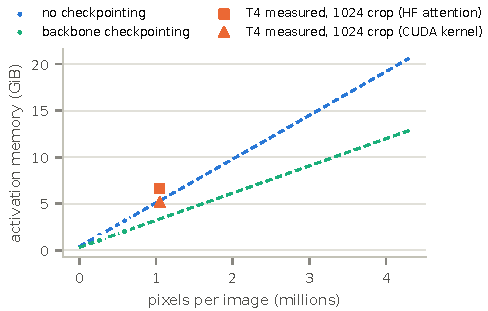
\includegraphics[width=0.62\textwidth]{figures/fig_memory.pdf}
\caption{The activation memory of the full Swin-S Mask2Former as a function of the number of pixels per
image, measured on a CPU at 512 and 768 pixels (dots, with linear fits) and on a T4 at 1024 pixels.
Recomputing the backbone's activations during the backward pass (checkpointing) saves about a third.
\generatedby{book/make\_book\_figures.py:fig\_memory}}
\label{fig:train-memory}
\end{figure}

\section{Faster kernels, proven identical *}\label{sec:train-kernels}
Three engineering changes made each training step faster. We required that no change to the speed may
change the mathematics, and we checked each change against the reference implementation before any
money was spent.

\subsection{A CUDA kernel for deformable attention}\label{sec:train-cuda}
Hugging Face computes the deformable attention of the pixel decoder (Equation~\eqref{eq:tr-deform}) with
a Python loop around \texttt{grid\_sample}. The same library ships a compiled CUDA kernel for the same
operation as part of its Deformable DETR model. We switched this kernel in, and compared it with the
reference on the shapes used in training, using random inputs whose sampling points extended slightly
beyond the edges of the feature maps. The outputs, and most of the gradients, agreed to within about
$10^{-5}$ in relative terms. The gradient with respect to the sampling \emph{locations} did not: at
2048 pixels its largest error was 1.2\%.

The cause turned out to be a property of bilinear interpolation (Figure~\ref{fig:train-kink}). A
bilinear sample is a continuous function of its location, but its derivative with respect to the
location jumps at every pixel centre. A point that lies within a millionth of a pixel of a centre can
land on either side of it, depending on how float32 arithmetic rounds its coordinates, and its gradient
then takes one value or the other. The test that settled the question computed a reference in float64,
and measured, for every large error, how far the point lay from the nearest crossing of a pixel centre.
Every large error lay within $7\times10^{-6}$ pixels of such a crossing, and the reference's \emph{own}
float32 loop showed the same errors in the same places. Away from the crossings, the kernel agreed with
the reference to $7\times10^{-6}$. Listing~\ref{lst:train-kernel} shows the essential part of the test.

\begin{figure}[t]
\centering
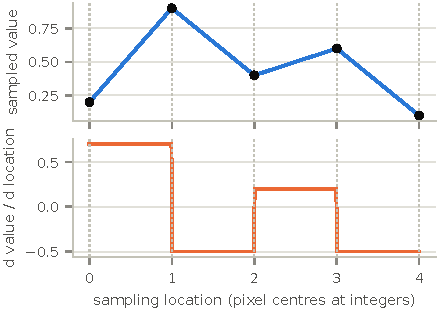
\includegraphics[width=0.62\textwidth]{figures/fig_kink.pdf}
\caption{Bilinear sampling along one axis. The sampled value (top) is continuous in the sampling
location, but its derivative (bottom) jumps at every pixel centre, so a gradient evaluated at a point
very close to a centre depends on which side of the centre rounding places the point.
\generatedby{book/make\_book\_figures.py:fig\_kink}}
\label{fig:train-kink}
\end{figure}

\begin{lstlisting}[caption={The kernel check: a float64 reference, and large errors allowed only at
kinks. Condensed from \file{experiments/exp\_139\_mask2former/src/fast\_ops.py}.},label=lst:train-kernel]
for name, function, dtype in (("truth", REFERENCE_MSDA, torch.float64),
                              ("kernel", kernel, torch.float64),
                              ("hf_float32", REFERENCE_MSDA, torch.float32)):
    inputs = [t.detach().to(device=device, dtype=dtype).clone().requires_grad_(True)
              for t in (value, locations, weights)]
    output = function(inputs[0], shapes, inputs[1], inputs[2])
    output.backward(grad_output.to(device=device, dtype=output.dtype))
    results[name] = [output.detach().double()] + [t.grad.double() for t in inputs]
# distance of every sampling point from the nearest pixel-centre crossing, per level
x = grid[..., 0] * widths - 0.5
y = grid[..., 1] * heights - 0.5
distance = torch.minimum((x - x.round()).abs(), (y - y.round()).abs())
near = distance < 1e-3                  # errors here are rounding at a kink, not a bug
passed = (errors["output"] <= 1e-4 and errors["grad_value"] <= 1e-4
          and errors["grad_weights"] <= 1e-4
          and errors["grad_locations_away_from_kinks"] <= 1e-4)
\end{lstlisting}

\subsection{Batched matching}\label{sec:train-matching}
The Hugging Face matcher copies one cost matrix from the GPU to the CPU for every image and for every
one of the ten predictions per step, which amounts to 80 stalls per step at a batch size of 8. Our
replacement computes all the matrices first, copies them once, and solves them on the CPU. We proved it
identical to the reference, bit for bit, on the loss and on all 161 gradient tensors of a small test
model, including the random draws of sampling points, which were made in the reference's order. On a
T4 it saved no measurable time, and we kept it only because it was proven harmless.

\subsection{A faster data loader}\label{sec:train-loader}
Our final loader decodes the photographs once into shared memory before the loader's worker processes
start. It decodes each annotated mask once and keeps only the crop of its bounding box, and it applies
the brightness augmentation and the normalisation on the GPU, starting from 8-bit pixels. A key-by-key
comparison with the first loader found no differences in the masks, and differences in pixel values
below $10^{-6}$, caused by float32 rounding in the gamma curve. The CPU time per sample fell from 80 to
19 milliseconds.

\subsection{How much faster?}\label{sec:train-speed}
The kernel reduced the time of a T4 step on two crops from 1.43 to 1.16 seconds, a speed-up of 1.24.
Profiling also corrected a guess that we had made beforehand. We had expected a speed-up of 1.5 to 2.5
times, but deformable attention accounted for only about a quarter of a step, so no kernel for it could
have delivered that.

\section{Exact gradient accumulation *}\label{sec:train-accumulation}
The final run used a batch of 8 in a single forward pass on a GPU with 80 GB or more of memory.
Cheaper cards with 24 GB could hold only two crops at a time, and the standard remedy for this,
\keyterm{gradient accumulation}, turned out to be subtly wrong for this loss.

Gradient accumulation splits a batch into $P$ micro-batches, runs the forward and backward passes on
each, and sums the gradients before taking a single optimiser step. The usual recipe divides the loss of
each micro-batch by $P$. This reproduces the full batch only if the loss of each micro-batch is an
average over parts of equal size, and the loss of Mask2Former is not. Its mask and Dice terms are
divided by the number of annotated masks \emph{in the current forward pass}, $n_b$, and its class term
by the total class weight in that pass, $w_b$, which counts one for each matched query and 0.1 for
each unmatched one. The loss of the whole batch is
\begin{equation}
\mathcal{L} = \frac{1}{N}\sum_b S^{\text{mask}}_b + \frac{1}{W}\sum_b S^{\text{cls}}_b,
\qquad N = \sum_b n_b,\quad W = \sum_b w_b,
\end{equation}
where $S^{\text{mask}}_b$ and $S^{\text{cls}}_b$ are the unnormalised sums of micro-batch $b$. Each
micro-batch reports the losses $\mathcal{L}^{\text{mask}}_b = S^{\text{mask}}_b/n_b$ and
$\mathcal{L}^{\text{cls}}_b = S^{\text{cls}}_b/w_b$, so the exact recombination weights each of them by
its \emph{share} of the batch:
\begin{equation}
\mathcal{L} = \sum_b \Big(\frac{n_b}{N}\,\mathcal{L}^{\text{mask}}_b + \frac{w_b}{W}\,\mathcal{L}^{\text{cls}}_b\Big).
\label{eq:train-shares}
\end{equation}
Dividing by $P$ instead would give a micro-batch containing one filament as much weight as one
containing twenty. Listing~\ref{lst:train-shares} implements Equation~\eqref{eq:train-shares}.

\begin{lstlisting}[caption={Scaling each micro-batch by its exact share. Condensed from
\file{experiments/exp\_139\_mask2former/src/train.py}.},label=lst:train-shares]
def step_shares(classes, num_queries, eos):
    masks = sum(len(item) for item in classes)                          # n_b
    weight = sum(len(item) + eos * (num_queries - len(item)) for item in classes)   # w_b
    return float(masks), float(weight)

def step_losses(model, pending, captured):
    counts = [step_shares(classes, 100, 0.1) for _, _, classes in pending]
    total_masks = sum(c[0] for c in counts)                            # N
    total_weight = sum(c[1] for c in counts)                           # W
    for (pixels, masks, classes), (n_b, w_b) in zip(pending, counts):
        model(pixel_values=pixels, mask_labels=masks, class_labels=classes)
        loss = sum(term * (w_b / total_weight if "cross_entropy" in key else n_b / total_masks)
                   for key, term in captured["dict"].items())          # the exact shares
        loss.backward()                                                # gradients accumulate
\end{lstlisting}

We tested the two recipes on a CPU with a small model, deterministic point sampling, and four samples
containing 6, 5, 1 and 1 filaments, split into two micro-batches, and measured the difference from a
single full batch:
\begin{center}\small
\begin{tabular}{@{}lcc@{}}
\toprule
accumulation & difference in loss & difference in gradient norm \\
\midrule
exact shares (Equation~\ref{eq:train-shares}) & $9.8\times10^{-8}$ & $1.4\times10^{-6}$ \\
division by the number of parts & $1.5\times10^{-3}$ & $4.1\times10^{-1}$ \\
\bottomrule
\end{tabular}
\end{center}
With exact shares, a card with 24 GB can train the same model that a larger card trains, at a fraction
of the price. This is what makes a cheaper run on the full data possible (Section~\ref{sec:sub-next}).

\section{The training run}\label{sec:train-run}
We trained the model on a rented H100 NVL GPU with 94 GB of memory, at \$2.59 an hour, with a spending
cap of \$6.50. The first attempt failed 53 seconds after training began. The machine's image set an
environment variable that asked the Hugging Face downloader to use an accelerator package which the
image did not contain. Our free rehearsals on Kaggle could not have caught this, because Kaggle does not
set that variable. Every check before that point had passed on the rented machine itself, including the
check that our scorer reproduces a known validation score to every printed digit. The fix was a single
environment variable, and the failed attempt cost about ten cents.

The second attempt ran all 50 epochs: 12,150 steps with a batch of 8, each in a single forward pass,
with no gradient accumulation and no activation checkpointing. Before its first step it checked the
CUDA kernel against the reference on the H100. After 45 steps it measured 0.464 seconds per step,
projected a total cost of \$5.25 including a reserve, and committed to all 50 epochs. It held 0.47
seconds per step and 39.35 GiB of memory throughout, and every five epochs it scored the validation
split (Figure~\ref{fig:train-curve}):
\begin{center}\footnotesize
\setlength{\tabcolsep}{3.5pt}
\begin{tabular}{@{}lcccccccccc@{}}
\toprule
epoch & 5 & 10 & 15 & 20 & 25 & 30 & 35 & 40 & 45 & 50 \\
\midrule
validation PQ & 0.420 & 0.420 & 0.441 & 0.444 & 0.440 & 0.457 & 0.460 & \textbf{0.468} & 0.467 & 0.464 \\
\bottomrule
\end{tabular}
\end{center}

\begin{figure}[t]
\centering
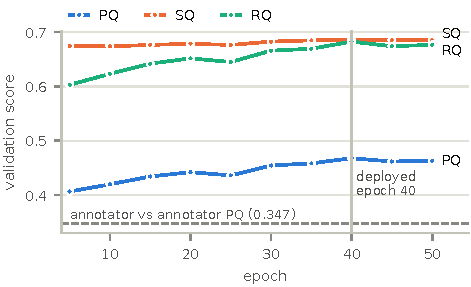
\includegraphics[width=0.7\textwidth]{figures/fig_curve.pdf}
\caption{Validation PQ, SQ and RQ of the final run, scored every five epochs during training, with
inference in bfloat16. PQ peaks at epoch 40, and the gains and losses late in training are mostly in
recognition. \generatedby{paper/make\_figures.py}}
\label{fig:train-curve}
\end{figure}

Two features of this curve deserve comment. First, the model improved until epoch 40, and then declined
slightly as the learning rate approached zero: at epoch 50 it found fewer filaments (813 true positives
against 872) and made fewer false detections. Second, epoch 40 was \emph{chosen} on the same validation
split on which it is scored. The best of ten candidates is optimistic by some amount, so the reported
score of 0.4705 includes the effect of this selection. The leaderboard, which played no part in the
selection, showed 0.41 for epoch 40 and 0.40 for epoch 50.

The whole run, including the failed first attempt, cost about \$4.80. The weights, 275,763,231 bytes per
checkpoint, were uploaded to a private Kaggle dataset, and we checked the dataset's listing before
deleting the rented machine.

A later run (exp142), intended to train on all 1,154 records, stopped within minutes on three rented
machines in a row. Our first diagnosis, which we wrote into the log, was that the account had run out of
credit. It was wrong. The diagnostics that the run itself had uploaded showed a
\texttt{ZeroDivisionError}: the projection of the budget divided by the interval between evaluations,
which a run on the full data sets to zero, and the machine's error handler had then stopped the machine,
as it was designed to do. The diagnostics that a failed run leaves behind should be read before the
infrastructure is blamed.

\section*{Exercises}
\begin{exercise}{Grid ceilings}
Reproduce the table of Section~\ref{sec:train-resolution} for cells of 2, 4 and 8 pixels on 200
training annotations: average each mask onto the coarse grid, enlarge it bilinearly, threshold it at
one half, and compute its IoU with the original. Then repeat the calculation with a binary encoding, in
which a cell is on if it is more than half covered, and compare the results.
\end{exercise}

\begin{exercise}{Steps per epoch}
With 974 records, two crops per record per epoch, and eight crops (or their equivalent) per step, how
many optimiser steps does an epoch have, and how many of them use whole frames? How many whole-frame
steps does the full run take?
\end{exercise}

\begin{exercise}{Clipping and Adam}
Show that if every gradient is multiplied by the same constant $c>0$, the update of
Equation~\eqref{eq:train-adamw} does not change, if we ignore $\epsilon$ and the weight decay. Then
explain what clipping every step to a fixed norm \emph{does} change.
\end{exercise}

\begin{exercise}{Accumulation by shares}
Two micro-batches contain 1 and 11 annotated masks, and their mask losses are 0.9 and 0.3. What is the
mask loss of the full batch, and what does dividing by the number of parts give instead?
\end{exercise}

\begin{exercise}{The kink}
Write bilinear interpolation along one axis, and its derivative with respect to the sampling location.
Evaluate the derivative in float32 at points $10^{-7}$ pixels on either side of a pixel centre, and
show that the two values differ by the difference between the neighbouring slopes.
\end{exercise}

\chapter{From Queries to a Submission, and How Good It Is}\label{ch:submission}

\section{Introduction}\label{sec:sub-intro}
\epigraph{Our judging committee will look at individual predictions, as well as the logic of the
algorithm.}{The competition's host, in the competition forum, 2026}

A trained network is not yet a submission. In this chapter we describe the path from the weights of
epoch 40 to the CSV file that the leaderboard scored (Section~\ref{sec:sub-path}), and the checks that
the deployment code performs before it writes any prediction (Section~\ref{sec:sub-replay}). We then
evaluate the resulting model: with the organisers' own scoring code (Section~\ref{sec:sub-eval}), by
looking at its predictions (Section~\ref{sec:sub-quality}), and by comparing it with the variants that
did not beat it (Section~\ref{sec:sub-variants}). We end with the next steps that our measurements
suggest (Section~\ref{sec:sub-next}).

\section{From weights to a CSV file}\label{sec:sub-path}
Between the weights of epoch 40 and the submitted file lie five steps, summarised in
Algorithm~\ref{alg:sub-emit}. Every one of them is shared, line for line, between validation and
deployment.

\begin{algorithmblock}{From a trained Mask2Former to a submission file\label{alg:sub-emit}}
\item \textbf{predict:} run the network on the native photograph in float32, and turn every query whose class probability exceeds a low floor (0.02) into a candidate, with a score from Equation~\eqref{eq:tr-score} and a binary mask of $2048\times2048$ pixels (Listing~\ref{lst:tr-predict});
\item \textbf{select:} keep the candidates whose score is at least the confidence threshold;
\item \textbf{paint:} give every pixel to the highest-scoring candidate that claims it, so that the masks become disjoint (Section~\ref{sec:masks-paint});
\item \textbf{filter:} drop the painted pieces that are smaller than the minimum area;
\item \textbf{encode:} write each remaining mask as a run-length encoding in one row of the CSV file (Section~\ref{sec:masks-rle})
\end{algorithmblock}

Listing~\ref{lst:sub-emit} shows the selection, painting and filtering steps as the code implements
them.

\begin{lstlisting}[caption={The emission rule, shared by validation and deployment. Condensed from
\file{experiments/exp\_139\_mask2former/src/submit.py:emit}.},label=lst:sub-emit]
def emit(entries, conf=0.85, grow=0, min_area=100):
    """exp033 sweep's emission, operation for operation, so the validated rule deploys unchanged."""
    candidates = []
    for entry in entries:                                   # entry: {score, rle}
        if entry["score"] < conf:
            continue
        mask = mu.decode(entry["rle"])
        if grow < 0:
            mask = cv2.erode(mask, KERNEL, iterations=-grow)   # never used by the final rule
        candidates.append((entry["score"], mask))
    painted = paint_panoptic(candidates, min_area=min_area)     # disjoint, highest score first
    return [encode(mask) for _, mask, _ in painted]
\end{lstlisting}

\subsection{Choosing the operating point}\label{sec:sub-operating}
The rule has three settings: the confidence threshold, an optional erosion, and the minimum area. We
chose them with the same sweep that we used to score every model in this book: 19 thresholds from 0.05
to 0.95, with and without a one-pixel erosion, and a minimum area of 100 or 300 pixels, making 76 rules
in all, each scored with the exact pooled PQ on the 180 validation records.

The sweep relies on a useful property of painting. Painting proceeds in order of decreasing score,
so raising the threshold only removes candidates from the \emph{end} of the painting order, and the
masks painted before them do not change. The set emitted at any threshold is therefore a prefix of the
set emitted at the lowest threshold, and all 19 thresholds can be scored from a single painting
(Exercise~\ref{ex:sub-prefix} asks for a proof). A unit test checks this equivalence.

The best rule for the final model used a threshold of 0.85, no erosion and a minimum area of 100
pixels. Two features of this rule fit what we know about the model. The threshold is high, which is
consistent with the calibration measurement of Section~\ref{sec:tta-calibration}, where we found the
Mask2Former's scores to be over-confident in the middle of their range. And the best erosion is none,
which is consistent with how its masks were trained: on \texttt{pycocotools} targets, which, unlike
the targets of the early YOLO models, are not systematically too wide.

\section{Replay before release}\label{sec:sub-replay}
The submission kernel ran on a free Kaggle T4. Before writing a single test prediction, it verified the
SHA-256 hash of the checkpoint against the manifest of the training run, re-checked the deformable
attention kernel on the T4, re-ran the validation with the deployment code, and required the result to
match the training run's validation score to within 0.005. The replay in float32 scored 0.47052,
against 0.46801 in bfloat16 during training, which was within the tolerance and slightly better. It also
measured eight-view test-time augmentation, which scored 0.46792 (with 39 more true positives and 102
more false positives), and chose the single view. Only then did it predict the 180 test photographs. It
produced 1,192 instances, recorded the SHA-256 hash of the CSV file, and drew a sheet of crops at the
native resolution for a person to inspect before anything was submitted. The file appeared on the
leaderboard as 0.41.

The replay exists because of a mistake described in Section~\ref{sec:val-traps}: a fusion rule that
was validated with one setting and prepared for deployment with another, which would have submitted
979 rows where the validated rule gave 1,229. The cure is structural. The deployment path imports the
functions of the validation path instead of re-implementing them, and it refuses to write test
predictions until it has reproduced a validated number.

\section{Scoring with the organisers' own code}\label{sec:sub-eval}
The competition's hosts published a self-evaluation notebook, and in exp145 we ran it without any
modification on the final model's validation predictions, recording its SHA-256 hash so that any
change to the notebook would be visible. It returned a PQ of 0.4705249989, and our own evaluator
returned 0.4705249990, with identical counts of true positives, false positives and false negatives.
Every validation number in this book therefore measures the quantity that the leaderboard measures.

\begin{figure}[t]
\centering
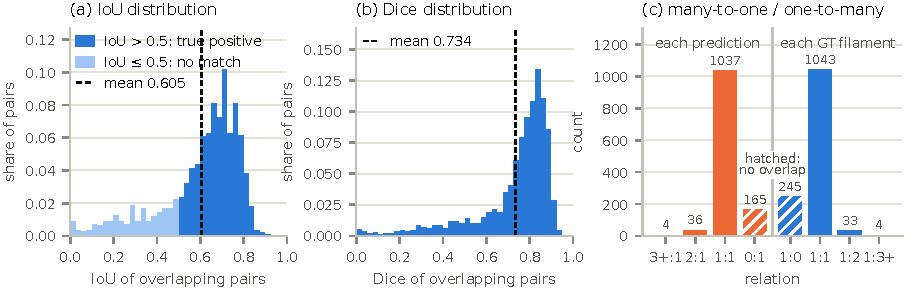
\includegraphics[width=\textwidth]{figures/fig_host_metrics.pdf}
\caption{The measures computed by the organisers' notebook on the final model's validation
predictions. (a) The IoU of every overlapping pair of annotation and prediction; the darker bars lie
above 0.5 and count as true positives. (b) The Dice coefficient of the same pairs. (c) How many
predictions touch each annotated filament (right), and how many filaments touch each prediction
(left); the hatched bars have no overlap at all. \generatedby{paper/make\_figures.py}}
\label{fig:sub-host}
\end{figure}

The results are summarised in the following table:
\begin{center}\small
\begin{tabular}{@{}lccc@{}}
\toprule
 & PQ & SQ & RQ \\
\midrule
final model, epoch 40 & \HostPQ{} & \ValSQ{} & \ValRQ{} \\
\quad 95\% bootstrap interval & [\PQLow{}, \PQHigh{}] & [\SQLow{}, \SQHigh{}] & [\RQLow{}, \RQHigh{}] \\
\quad TP / FP / FN & \multicolumn{3}{c}{\NumTP{} / \NumFP{} / \NumFN{}} \\
annotator against annotator & \HumanPQ{} & \HumanSQ{} & \HumanRQ{} \\
\quad 95\% bootstrap interval & [\HumanPQLow{}, \HumanPQHigh{}] & & \\
public leaderboard (test) & \BestPublic{} & -- & -- \\
\bottomrule
\end{tabular}
\end{center}
The intervals come from the bootstrap of Section~\ref{sec:metric-uncertainty}, which resamples the
\ValPhotos{} validation photographs 10,000 times, keeping the records of each photograph together. The
row for the annotators scores every annotator against every other annotator of the same validation
photographs, under the same rule. As Section~\ref{sec:metric-agreement} explained, the model's higher
score does not mean that it is more skilled than an expert. A model trained on many annotators learns
something like their average, and an average can lie closer to each person than two people lie to each
other.

Figure~\ref{fig:sub-host} adds the distributions that the organisers' notebook reports. The overlapping
pairs have a mean IoU of \MeanIoUOverlap{} and a mean Dice coefficient of \MeanDiceOverlap{}. Of the
annotated filaments, \GTOneOnePct{}\% touch exactly one prediction, \GTSplitPct{}\% touch two or more,
and \GTMissedPct{}\% touch none. Of the predictions, \PredOneOnePct{}\% touch exactly one filament,
\PredMergePct{}\% touch two or more, and \PredUnmatchedPct{}\% touch none.

In a reply in the competition's discussion forum, the host wrote that ``anything beyond 3.5 PQ is of
great interest to us''. Since PQ lies between 0 and 1, the number cannot be meant literally, and we have
recorded it as written without guessing what was intended. The same reply said that the judges will
look at individual predictions and at the logic of the algorithm, and not only at the score, and the
next section therefore looks at pictures.

\section{What the model gets right, and what it misses}\label{sec:sub-quality}
A summary number hides the individual predictions, so we now look at them. To avoid choosing a
flattering example, we selected the photograph for Figure~\ref{fig:sub-qual} by a fixed rule: among the
validation photographs that have a single annotator and at least eight filaments, it is the one whose
PQ is closest to the median. It is therefore a typical case.

\begin{figure}[t]
\centering
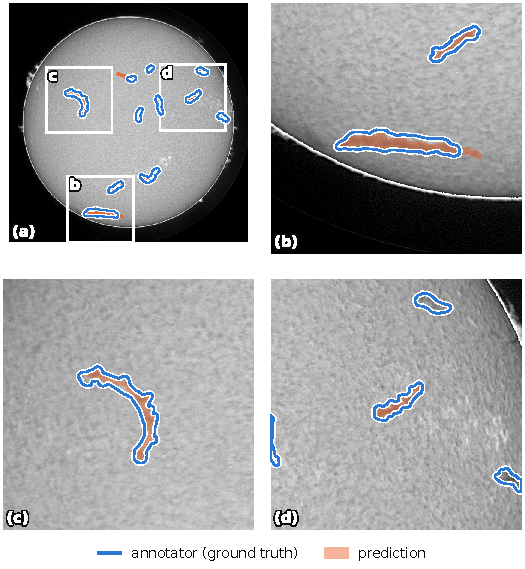
\includegraphics[width=\textwidth]{figures/fig_qualitative.pdf}
\caption{The validation photograph whose PQ (\QualPQ{}) is closest to the median of the
\QualCandidates{} single-annotator photographs with at least eight filaments (median \QualMedian{}).
(a) The full disk. (b)--(d) Zooms at the native resolution on the three largest annotated filaments.
Blue shows the annotation, outlined outside the mask so that the outline never covers it; orange shows
the model's prediction. \generatedby{paper/make\_figures.py}}
\label{fig:sub-qual}
\end{figure}

\paragraph{Strengths.} The model rarely splits or merges filaments: \GTSplitPct{}\% of the annotated
filaments touch more than one prediction, and \PredMergePct{}\% of the predictions touch more than one
filament. This is the set-prediction property of Section~\ref{sec:tr-detr} showing up in the counts.
Once a filament is found, its mask is good (SQ \ValSQ{}), and the boundaries follow the dark body without
the systematic widening that the early YOLO models needed erosion to remove. A review of validation
predictions at the native resolution, made before submission, found that the model detects large and
medium filaments reliably, including long curved ones. The whole test set runs in about
\TestMinutes{} minutes on one T4 GPU, at \SecondsPerPhoto{} seconds per photograph and with
\PeakGiB{} GiB of memory.

\paragraph{Weaknesses.} The model misses more than it invents, with \NumFN{} false negatives against
\NumFP{} false positives. Figure~\ref{fig:sub-size} shows where the misses occur. Recall is
\RecallSmall{} for the smallest sixth of the filaments (those under \SmallArea{} pixels) and
\RecallLarge{} for the largest sixth, and precision follows the same trend. The misses are concentrated
on thin, faint filaments, several of them next to bright active regions.

\begin{figure}[t]
\centering
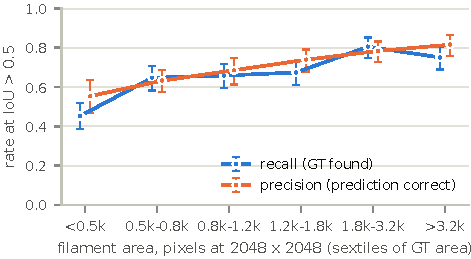
\includegraphics[width=0.7\textwidth]{figures/fig_size.pdf}
\caption{Recall (the fraction of annotated filaments found with an IoU above 0.5) and precision (the
fraction of predictions that match) as functions of filament area, in sixths of the annotated areas
(\PerBin{} filaments each). The bars are Wilson 95\% intervals (Section~\ref{sec:metric-uncertainty}).
\generatedby{paper/make\_figures.py}}
\label{fig:sub-size}
\end{figure}

Figure~\ref{fig:sub-failures} shows one example of each kind of error, again chosen by a fixed rule: the
median-sized filament that no prediction touches, the median-sized prediction that touches no filament,
and the largest filament that is touched by several predictions. The first is small and faint. The
second is a dark structure that this annotator did not mark, the kind of candidate that
Chapter~\ref{ch:recall} found so hard to judge. The third is a long filament covered in several pieces.

\begin{figure}[t]
\centering
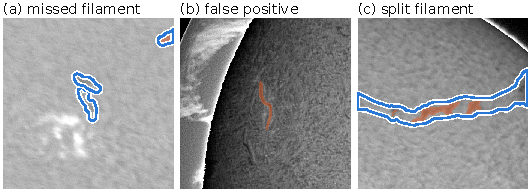
\includegraphics[width=\textwidth]{figures/fig_failures.pdf}
\caption{One example of each kind of error, chosen by a fixed rule over single-annotator validation
records: (a) the filament of median area that no prediction touches; (b) the prediction of median area
that touches no filament; (c) the largest filament touched by two or more predictions. The colours are as
in Figure~\ref{fig:sub-qual}. \generatedby{paper/make\_figures.py}}
\label{fig:sub-failures}
\end{figure}

\section{Variants that did not beat it}\label{sec:sub-variants}
We validated four variations of the final model and, to settle each question, submitted them:
\begin{center}\small
\begin{tabular}{@{}lcc@{}}
\toprule
variant & validation PQ & public \\
\midrule
\textbf{epoch 40, one view (deployed)} & \textbf{0.4705} & \textbf{0.41} \\
epoch 50, one view & 0.4621 & 0.40 \\
weight soup of epochs 40 and 50 & 0.4688 & 0.40 \\
epoch 40, eight-view fusion & 0.4700 & 0.40 \\
calibrated ensemble with YOLOv8l & 0.4715 & 0.40 \\
\bottomrule
\end{tabular}
\end{center}
Chapter~\ref{ch:tta} explained each of them. The last row is a useful warning. Its validation score
was 0.001 \emph{higher} than that of the deployed model, which is below the margin of 0.005 that we had
fixed in advance, and the leaderboard ranked it lower. Differences of this size cannot be resolved by
either instrument.

\section{What would come next}\label{sec:sub-next}
Our measurements point to three next steps. These are proposals, and we have no results for them yet.
\begin{enumerate}[leftmargin=*,itemsep=2pt]
\item \textbf{Train on every record.} The final model never saw the 180 validation records. With the
recipe fixed, a run on all 1,154 records would add 180 records to the 974 used so far, about 18\% more.
The division by zero that stopped the first attempt (Section~\ref{sec:train-run}) has been fixed, exact
gradient accumulation lets a card with 24 GB train the same model, and a measured speed of 1.34 seconds
per step on an RTX 3090 puts 30 epochs at a cost of about \$0.71. Without a held-out split, however,
such a run can be judged only by its training behaviour and by the leaderboard, so the recipe must be
frozen before the run starts.
\item \textbf{A gate for the extra detections.} Eight-view fusion added 60 true positives and 125 false
positives. By the arithmetic of Section~\ref{sec:recall-arith}, a verifier that kept two thirds of the
true positives and a third of the false positives would turn this into a gain. Chapter~\ref{ch:recall}
shows how hard such a verifier is to build, and why it must be labelled per record.
\item \textbf{Consensus targets.} There are 296 photographs with two or three annotations. An earlier
test found that a consensus of two annotators predicted a third no better than a single annotator did
(0.3291 against 0.3287), so consensus labels are not an obvious gain. Whether they help a model to
\emph{learn}, as opposed to scoring it, has never been tested.
\end{enumerate}

\section*{Exercises}
\begin{exercise}{Prefix painting}\label{ex:sub-prefix}
Prove that for any two thresholds $c_1 < c_2$, the painted set at $c_2$ equals the painted set at $c_1$
restricted to the candidates with scores of at least $c_2$, including the effect of the minimum-area
filter. Where would the proof break if painting gave contested pixels to the \emph{larger} mask
instead of the higher-scoring one?
\end{exercise}

\begin{exercise}{Reading the interval}
The bootstrap interval for the model's PQ is [\PQLow{}, \PQHigh{}], and the calibrated ensemble scored
0.4715. Explain why the two models cannot be ranked from these numbers, and what a paired bootstrap of
their difference would measure instead.
\end{exercise}

\begin{exercise}{Small filaments}
Using the recall and precision of the smallest sixth of the filaments, estimate how much PQ would rise
if the recall in that bin matched the recall in the largest bin, at the same precision and SQ. Compare
your estimate with the gains in Figure~\ref{fig:tta-ensembles}.
\end{exercise}

\begin{exercise}{Look before you submit}
Write a function that, for one photograph, draws the annotated outlines and the emitted masks on crops at
the native resolution around each of the three largest annotated filaments, as in
Figure~\ref{fig:sub-qual}. Why should the outlines be drawn outside the masks rather than on them?
\end{exercise}

\chapter{Lessons: How This Project Could Have Fooled Itself}\label{ch:lessons}

\section{Introduction}\label{sec:lessons-why}
\epigraph{To consult the statistician after an experiment is finished is often merely to ask him to
conduct a post mortem examination. He can perhaps say what the experiment died of.}{Ronald Fisher,
address to the Indian Statistical Congress \citeyearpar{fisher1938}}

Most of our time went into experiments that failed, and a fair share of the failures were failures of
\emph{method} rather than of ideas: a setting that was not what we believed it to be, a number
measured in the wrong place, or a conclusion that went further than its evidence. The repository keeps
a list of these mistakes in its working notes (\file{CLAUDE.md}), written so that they would not be
repeated. In this chapter we organise that list into a small number of principles. None of the
principles is new: many of them appear in accounts of the hidden costs of machine-learning
systems~\citep{sculley2015} and of the ways in which machine-learning papers claim more than their
evidence supports~\citep{lipton2019}. What justifies a chapter is that each of them cost this project real time or money,
and each comes with a concrete example that shows how easily it is violated.

The principles fall into five groups: knowing what is actually running
(Section~\ref{sec:lessons-config}), measuring the right quantity in the right place
(Section~\ref{sec:lessons-measure}), asking the question that the metric asks
(Section~\ref{sec:lessons-question}), claiming no more than the evidence supports
(Section~\ref{sec:lessons-claims}), and spending limited resources deliberately
(Section~\ref{sec:lessons-spend}). Section~\ref{sec:lessons-checklist} condenses them into a checklist.

\section{Knowing what is actually running}\label{sec:lessons-config}

\paragraph{Configurations must be read back from the run.} We believed that exp010 was running with
full-resolution mask supervision (\texttt{mask\_ratio=1}), because its validation loop ran for 45
iterations, which implied a batch size of 2. But the batch size says nothing about the resolution of
the masks. The run's own \file{args.yaml} said \texttt{mask\_ratio: 2}, because a silent fallback had
changed the very setting that the experiment was designed to test, and twelve GPU hours measured the
wrong configuration (Section~\ref{sec:yolo-exp010}). After any run starts, we should read its resolved
configuration and confirm that it is the one we intended. \citet{sculley2015} discuss the errors
that accumulate in the configuration of machine-learning systems under the name
\emph{configuration debt}.

\paragraph{State must be queried again before it is reported.} On one occasion we reported a run as
healthy ``twenty minutes in'', on the basis of a status check that was already out of date; the run had
failed after five minutes. The state of a remote job changes, and a report about it should rest on a
fresh query.

\paragraph{A library is source code.} Ultralytics silently replaced a learning rate that we had
requested, resumed from a folder that nobody had chosen, and halved a batch after an out-of-memory error
(Section~\ref{sec:yolo-lessons}). A rented machine failed inside our own training callbacks, because
they had been written against an assumed version of the library's internals and tested only against
that assumption (Section~\ref{sec:yolo-exp097}). When our code touches a library's internals, we should
read those internals in the exact version that we pin, and rehearse the real code against that version
on free hardware before it costs money.

\paragraph{Before launching anything, list what is already running.} A handoff note stated that an
experiment ``was prepared but not launched'', and a status query for one guessed name seemed to confirm
it. In fact the experiment was running under a different name, which Kaggle had derived from its
title rather than from its identifier (Appendix~\ref{app:infra}). A duplicate was launched and ran for
ten minutes before anyone noticed. A query about one guessed name is not a check for running work, and
a claim that something was ``not launched'' should never be inherited from a note without checking it.

\section{Measuring the right thing, in the right place}\label{sec:lessons-measure}

\paragraph{The rule that is deployed must be the rule that was validated.} We validated a fusion rule
with its second model run at a confidence floor of 0.05, and then prepared it for deployment with the
floor at 0.30. The deployment file had 979 rows where the validated rule gave 1,229, and only the count
of rows revealed the mistake (Section~\ref{sec:val-traps}). The deployment path should import the
validation path, and it should reproduce a validated number before it writes anything
(Section~\ref{sec:sub-replay}).

\paragraph{Measurements belong at the metric's resolution.} A refiner's gain of $+0.0118$ at the level
of crops turned out to be an artefact of resampling, because the same measurement gave $+0.0117$ with
no model at all (Section~\ref{sec:post-v2}). We should measure at the resolution, on the population and
in the units that the metric uses: native pixels, all records, and pooled counts.

\paragraph{Every number comes from a stage of the pipeline.} The statement that ``284 misses have zero
overlap'' described the predictions emitted after the confidence floor, and not the output of the
detector; in the full pool of candidates only 65 of those filaments had never been proposed
(Section~\ref{sec:recall-stages}). A statistic measured downstream of a filter cannot describe what the
filter removed.

\paragraph{Like must be compared with like.} SQ is an average over matched pairs only. Comparing it with
a per-instance IoU averaged over all instances compares a filtered population with an unfiltered one, and
it once made our masks look as good as those of a published method when nothing of the kind had been
shown (Section~\ref{sec:metric-sq-properties}).

\paragraph{Memory experiments need separate processes.} When we tested several memory configurations in
one process, two of them produced byte-identical out-of-memory errors although the batch size between
them had halved. The second configuration had never run, because \texttt{torch.cuda.empty\_cache()}
cannot free memory that an earlier trainer still references, and every later measurement was
contaminated (Section~\ref{sec:yolo-exp031}). Each memory experiment should run in its own process, and
the allocator settings must be made before anything imports PyTorch.

\paragraph{Silence is not a result.} A script written without an
\texttt{if \_\_name\_\_ == "\_\_main\_\_"} block imported cleanly and did nothing, twice, and its
empty output could easily have been read as a negative result. We should check that a script actually
ran before interpreting its output.

\section{Asking the question the metric asks}\label{sec:lessons-question}

\paragraph{The training objective must ask the metric's question.} The crop verifier was labelled
positive if \emph{any} annotator had drawn a filament, whereas the metric asks whether \emph{this}
annotator drew it. The model was right 72\% of the time on the first question and 17\% of the time on
the second (Section~\ref{sec:recall-crop}). Before choosing labels, we should write down the exact
question that the metric asks.

\paragraph{A synthetic test that encodes an assumption cannot test it.} Snapping masks to the edge of
the intensity scored an IoU of 0.9995 on a synthetic filament and destroyed real masks, because the
synthetic filament had the hard edge whose existence was under test (Section~\ref{sec:post-free}). A
sanity check confirms that code runs; only real data can test an idea, and we should always say which of
the two we are doing.

\paragraph{An ablation needs headroom.} Two ablations of instance decoders were run on annotated masks,
where the control already scored 0.9995, so no decoder could have shown a gain
(Section~\ref{sec:par-headroom}). The score of the control should be computed first; if it is already at
the ceiling, the ablation cannot answer its question.

\paragraph{Ceiling, operator and gate, in that order.} Several repair ideas were dropped because their
triggers failed, before anyone had measured whether the repair itself was worth anything
(Section~\ref{sec:post-protocol}). A failed trigger says nothing about the repair that it was meant to
activate.

\section{Claiming no more than the evidence supports}\label{sec:lessons-claims}

\paragraph{A result about one side of the confusion matrix is a result about that side.} False positives
occurred at the rate at which annotators disagree with each other, and our notes extended this finding
to the misses, where it was false: only 2.1\% of the annotated filaments were invisible to the detector
(Section~\ref{sec:recall-orphans}). Later, after the verifier failed, the notes over-corrected in the
other direction. Two reversals on one question within a single day came from letting a measurement of one
quantity stand in for another.

\paragraph{Failed formulations are not a proof of impossibility.} After five methods for correcting
boundaries had failed, our notes declared the annotated boundary unrecoverable by any method applied
after prediction (Section~\ref{sec:post-overreach}). The measurements were sound, but the generalisation
was not. The competition's host has described uncertain boundaries as part of the physical problem,
and has encouraged participants to concentrate on the quality of their predictions rather than on the
score alone; nothing in that description implies that useful improvement is impossible.

\paragraph{Agreement between annotators is not a bound.} Two annotators agree with each other at a PQ of
0.34 and a mean IoU of 0.58. These numbers describe people. They do not limit what a model can score
against any one of them, and our model exceeds the first of them comfortably
(Section~\ref{sec:metric-agreement}).

\paragraph{The primary source should be read.} The abstract of the MAGFiLO paper reports 1,593
observations, which suggested that the public release could double our training data. The release in
fact holds 958 distinct photographs, of which the competition already uses 887, and it contains the
annotations of the test set (Section~\ref{sec:data-history}). The apparent doubling amounted to about 71
photographs, and using them would have been cheating.

\paragraph{The first explanation of a failure is a hypothesis.} We blamed rented machines that stopped
within minutes on an exhausted account. The diagnostics that the machines had uploaded showed a division
by zero in our own code (Section~\ref{sec:train-run}). The evidence that a failure leaves behind should
be read before its cause is named.

\section{Spending limited resources deliberately}\label{sec:lessons-spend}

\paragraph{Numbers already measured should change what we do.} Validation said that a fusion rule
changed 9 instances out of 1,238. We submitted it anyway, and it turned out to be 99.3\% identical to an
earlier submission. When a measurement says that a change is negligible, it should stop the spending.

\paragraph{A schedule should fit the session.} A cosine schedule sized for 400 epochs, but cut off at
epoch 62, never left its peak learning rate (Section~\ref{sec:yolo-exp010}). A short schedule that
anneals fully is better than a long one that is cut off (Section~\ref{sec:train-optim}).

\paragraph{A sweep should be costed before it runs.} Caching dense $2048\times2048$ masks for three levels
of erosion needed about 27 GB of memory, and the process was killed. Masks kept as run-length encodings
cost kilobytes, and \texttt{pycocotools} computes IoU on them directly (Section~\ref{sec:masks-rle}). In
another case, a grid of 120 points took hours, whereas a coarse grid followed by a fine one found the
same optimum in minutes.

\paragraph{The lifecycle that will actually happen is the one to test.} A plan to chain twelve-hour
Kaggle sessions relied on one session reading the output of the previous one. We tested this for a
session that had \emph{completed}. A training session, however, ends by reaching the time limit, and is
then \emph{cancelled}, and the output of a cancelled session cannot be mounted by the next one.

\paragraph{A watcher must check what has already been done.} A background loop waited for GPU quota and
then launched a training kernel. When the quota reset, we launched the kernel by hand, and the loop,
which was still running, came within two minutes of launching a duplicate. A watcher that acts must check
whether its action has already happened, and not only whether the action is possible.

\section{A checklist}\label{sec:lessons-checklist}
Figure~\ref{fig:lessons-flow} condenses the path that an idea followed during the better weeks of the
project, from its first formulation to a submission. Each step can end an idea cheaply, before the next
and more expensive step is taken.

\begin{figure}[t]
\centering
\begin{tikzpicture}[
  st/.style={box=#1, text width=5.2cm, minimum height=0.62cm, font=\sffamily\scriptsize,
             execute at begin node={\hyphenpenalty=10000}},
  why/.style={note, anchor=west, text width=4.9cm, align=left}]
  \node[st=inkmuted] (a) at (0,0) {write down the metric's exact question and the expected gain};
  \node[st=vizblue] (b) at (0,-0.95) {measure the family's ceiling with an oracle};
  \node[st=vizblue] (c) at (0,-1.9) {measure the operator under a perfect gate};
  \node[st=vizaqua] (d) at (0,-2.85) {build the real trigger; check its break-even rate};
  \node[st=vizaqua] (e) at (0,-3.8) {validate at native resolution, pooled, all records};
  \node[st=vizorange] (f) at (0,-4.75) {gain larger than its noise? paired bootstrap};
  \node[st=vizorange] (g) at (0,-5.7) {replay the validated number in the deployment path};
  \node[st=inkmuted] (h) at (0,-6.65) {look at native-resolution predictions; then submit};
  \foreach \u/\v in {a/b, b/c, c/d, d/e, e/f, f/g, g/h} \draw[flow] (\u) -- (\v);
  \node[why] at (3.1,0) {Chapter~\ref{ch:metric}; Section~\ref{sec:recall-crop}};
  \node[why] at (3.1,-0.95) {too small a ceiling: stop here};
  \node[why] at (3.1,-1.9) {operator recovers little: fix it or stop};
  \node[why] at (3.1,-2.85) {Equation~\eqref{eq:post-gate}};
  \node[why] at (3.1,-3.8) {Sections~\ref{sec:val-traps} and~\ref{sec:post-v2}};
  \node[why] at (3.1,-4.75) {the leaderboard cannot see less than about 0.01};
  \node[why] at (3.1,-5.7) {Section~\ref{sec:sub-replay}};
  \node[why] at (3.1,-6.65) {the hosts judge predictions, not only scores};
\end{tikzpicture}
\caption{The path from an idea to a submission. Each step can end the idea cheaply, before the next,
more expensive step is taken. \drawnin{book/chapters/ch14\_lessons.tex}}
\label{fig:lessons-flow}
\end{figure}

Three questions summarise the whole chapter, and we found it useful to ask them before believing any
number. First, where exactly was the number measured: at which stage of the pipeline, on which
population, at which resolution, and in which units? Second, what does the control score under the same
measurement? Third, what would the number have been if the idea had been worthless? Until all three
questions have answers, we do not yet know what the number means.

\section*{Exercises}
\begin{exercise}{Finding the configuration}
Choose any training run in \file{kaggle/} or \file{experiments/}. Find the file that records the
configuration with which it actually ran, and list every value that differs from the defaults in its
source code.
\end{exercise}

\begin{exercise}{A lesson of your own}
Choose one experiment from Appendix~\ref{app:ledger} whose conclusion you find surprising. Write down the
measurement that supports it, the population and resolution at which the measurement was taken, and one
way in which the conclusion could be wrong.
\end{exercise}

\begin{exercise}{Designing a watcher}
Write pseudocode for a background job that waits for a Kaggle kernel to finish and then submits its
output. List every condition that it must check before submitting, including those that this chapter's
examples suggest.
\end{exercise}


\appendix
\chapter{Infrastructure: Kaggle and RunPod}\label{app:infra}

\section{Where the computing happens}\label{sec:infra-where}
Almost none of the computation in this project runs on the computer that holds the repository. From
15 September 2026 onwards we followed an explicit rule: nothing is downloaded to the local machine,
and no local bandwidth is spent. Code is written locally, shipped to remote machines and run there,
and only small artefacts, such as reports, CSV files, figures and PDF documents, come back. We used two
kinds of remote machine: Kaggle kernels, which are free within a weekly quota, and GPUs rented from
RunPod, which are paid for by the hour.

\section{Kaggle kernels}\label{sec:infra-kaggle}
A Kaggle \keyterm{kernel} (which Kaggle now also calls a notebook) is a script that Kaggle runs on its
own hardware, with the competition data and any chosen datasets mounted read-only under
\file{/kaggle/input}. The following facts about kernels shaped how we worked.
\begin{itemize}[leftmargin=*,itemsep=2pt]
\item \textbf{Hardware.} Kaggle offers kernels with CPUs only, with one or two NVIDIA T4 GPUs (16 GB
each), or with a TPU v5e with eight cores. During the project our account had about 30 GPU hours and
20 TPU hours per week, one TPU session at a time, and a limit of 12 hours per session.
\item \textbf{Outputs.} Only the files written under \file{/kaggle/working} survive a session. An early
experiment lost 1.5 hours of training because it wrote its checkpoints to \file{/kaggle/temp}.
\item \textbf{Metadata.} Each kernel folder contains a file \file{kernel-metadata.json}, which names
the script, the datasets and other kernels to mount, and whether a GPU and internet access are enabled.
Kaggle derives the address of a kernel (its ``slug'') from its \emph{title}, not from the \texttt{id}
field of this file. When the two disagree, a push can land at an address that no later status query
looks at, so we keep them identical.
\item \textbf{Knowing what runs.} The command \texttt{kaggle kernels list --user <user> --sort-by
dateRun} lists the kernels that actually ran. A status query for a single guessed name is not a
reliable check (Section~\ref{sec:lessons-config}).
\item \textbf{Chaining sessions.} A kernel can mount its own earlier output, which in principle allows
twelve-hour sessions to be chained. However, a kernel that is stopped by the time limit is
\emph{cancelled}, and the output of a cancelled kernel cannot be mounted. Any plan that relies on
chaining must be tested on that path.
\item \textbf{CPU and GPU agree.} Inference on Kaggle's CPUs produced a submission file identical, bit
for bit, to the one produced by inference on a GPU (the two files had the same MD5 hash). We therefore
used CPU kernels freely for inference and scoring, and kept the GPU hours for training.
\end{itemize}

\subsection{TPUs}\label{sec:infra-tpu}
Kaggle's TPU trained the dense U-Nets well: exp004 ran 300 epochs at 1024 pixels in 3.8 hours. It used
a single Python process with SPMD sharding across the eight cores, because the usual launcher, which
starts one process per core, failed while the TPU was starting up on Kaggle's image. The XLA compiler
recompiles the model for every new tensor shape, so the batches had to have fixed shapes, and every
call to \texttt{.item()} stalls the pipeline, so we read the losses only once per epoch. YOLO training
never ran on the TPU, because compilation timed out, and the first Mask2Former trained there far too
slowly to finish (Section~\ref{sec:train-first}).

\section{Datasets as a means of transport}\label{sec:infra-datasets}
Private Kaggle datasets carry code to the remote machines and bring weights back. Two properties of
Kaggle's datasets determined how we use them.
\begin{itemize}[leftmargin=*,itemsep=2pt]
\item \textbf{Kaggle unpacks archives.} After an upload, a \file{.tar.gz} file is listed as the files
it contains, so a single archive whose SHA-256 hash a remote machine intended to check no longer
exists. We therefore ship code as a tar archive renamed to \file{.payload}, and the receiving machine
verifies its SHA-256 hash before running anything.
\item \textbf{The listing must be checked.} After every upload we list the dataset's files and their
sizes, and compare them with what we intended to upload, before anything depends on the dataset.
\end{itemize}
On Windows, the version of the Kaggle command-line tool that we used failed on \texttt{-p} arguments
containing forward slashes; running the tool from inside the folder with \texttt{-p .} avoided the
problem. Downloading the logs of a kernel required setting \texttt{PYTHONUTF8=1}, because otherwise a
single non-ASCII character in the log produced an empty file.

\section{RunPod}\label{sec:infra-runpod}
We trained two models on rented GPUs:
\begin{center}\small
\begin{tabular}{@{}llccc@{}}
\toprule
experiment & GPU & per hour & length & cost \\
\midrule
exp097 (YOLOv8l-seg) & L40, 48 GB & \$0.69 & 124 epochs & \$2.74 \\
exp139 (Mask2Former) & H100 NVL, 94 GB & \$2.59 & 50 epochs & about \$4.80 \\
\bottomrule
\end{tabular}
\end{center}
Two early machines for exp097 that failed before training began added \$0.22 to the cost.

A rented machine starts from a standard PyTorch image and runs a bootstrap script. The script downloads
the code payload from a private Kaggle dataset, checks its SHA-256 hash, reproduces a known validation
score to prove that the scorer works on that machine, runs a short preflight that measures speed and
memory, and only then starts training. Checkpoints are uploaded to a private Kaggle dataset, whose
listing the machine verifies before it stops itself. If any command fails, an error handler uploads the
logs and stops the machine, so that a failure costs minutes rather than hours. For the same reason, the
diagnostics that a failed machine uploads, and not the provider's own log, are the place to look for the
cause of a failure (Section~\ref{sec:train-run}).

The Kaggle access key reaches a rented machine only through its environment, when the machine is
created, and it is never written to a file in the repository or to a log. Spending is bounded in two
ways: the trainer projects its cost from its measured speed and stops at a cap, and the hourly price of
every new machine is stated and approved before the machine is created.

\section{Submitting and watching}\label{sec:infra-submit}
A submission is a single command:
\begin{lstlisting}[language=bash,caption={Submitting a CSV file to the competition.},label=lst:infra-submit]
kaggle competitions submit -c filament-segmentation-2026 -f submission.csv -m "exp139 epoch 40 ..."
\end{lstlisting}
The message attached to a submission has a practical use. The script
\file{scripts/watch\_and\_submit.sh} polls kernels, downloads each finished submission file and submits
it, and it decides whether a file has already been submitted by comparing messages. An earlier version
compared file names instead, and since every kernel calls its output \file{submission.csv}, it skipped a
new file because an old submission had the same name. Finally, \file{scripts/alarm.ps1} plays a sound and
shows a window when a long job ends:
\begin{lstlisting}[language=bash,caption={The end-of-job alarm on Windows.},label=lst:infra-alarm]
powershell -ExecutionPolicy Bypass -File scripts\alarm.ps1 -Message "book built" -Seconds 15
\end{lstlisting}

\chapter{The Experiment Ledger}\label{app:ledger}

This appendix lists our experiments in the order in which they were run, together with the result
that decided each one and the chapter that describes it. Validation numbers are PQ on the canonical split
(Chapter~\ref{ch:validation}); ``public'' is the leaderboard's two-decimal score. The full record of
each experiment is in \file{docs/leaderboard-analysis.md} (up to exp031) and
\file{docs/ACTIVE\_EXPERIMENT.md} (from exp033).

{\small
\setlength{\tabcolsep}{4pt}
\begin{longtable}{@{}>{\raggedright\arraybackslash}p{1.95cm}>{\raggedright\arraybackslash}p{5.5cm}>{\raggedright\arraybackslash}p{3.9cm}>{\raggedright\arraybackslash}p{0.75cm}@{}}
\toprule
experiment & what was tried & decisive result & ch. \\
\midrule
\endfirsthead
\toprule
experiment & what was tried & decisive result & ch. \\
\midrule
\endhead
\bottomrule
\endfoot
exp001 & U-Net++ (EfficientNet-B4) at 512, semantic mask then connected components & 0.2957; public 0.26 & 6 \\
exp002 & YOLO11m-seg at 1280, 149 epochs, stopped by a time budget & 0.3736 tuned; public 0.32 & 7 \\
exp002 & the same weights, inference at the native 2048 & 0.4064; public 0.33 & 7 \\
exp004 & U-Net (ResNet-34) at 1024, 300 epochs on TPU, flip averaging & public 0.28 & 6 \\
exp004 & spine-seeded instances, ablated on degraded annotations & $+0.0005$; dropped & 6 \\
exp005 & centre and offset grouping, ablated with noisy offsets & $\le 0$; dropped & 6 \\
exp005 & erode every mask by one pixel, confidence 0.35 & 0.4404; public 0.36 & 7 \\
exp005 & gradient-boosted emission over shape features & $-0.017$ against confidence & 10 \\
exp006 & rasteriser comparison; half-pixel polygon offset & target IoU 0.898 $\to$ 0.959 & 3, 7 \\
exp007 & first eight-view TTA, binary vote & 0.4035; lost & 8 \\
exp008, 009 & crop refiner trained on synthetic damage & 0.4322 ($-0.008$); public 0.35 & 9 \\
exp010 & YOLO11m at 2048 on a T4; fell to \texttt{mask\_ratio} 2; 62 of 400 epochs & 0.4274; public 0.36 & 7 \\
exp011, 012, 018 & refiner trained on 3,429 real detector errors & learned the identity; $-0.031$ & 9 \\
exp013 & error decomposition with oracles & orphans: 49\% of FP, 59\% of FN & 9, 10 \\
exp014 & orphan rates of the model and of annotators & 19.8\% against 19.4\% & 10 \\
exp015 & CPU inference path & bit-identical to GPU & A \\
exp016 & recall ceiling of the pool at confidence 0.05 & 83.2\% covered, 2.1\% unseen & 10 \\
exp017 & sub-pixel trim by a higher cut on the logit field & no better than erosion & 9 \\
exp019 & re-ranker on the logit-field profile & promotes nothing & 10 \\
exp021, 023 & second YOLO as a veto on the first & $+0.0007$; public 0.36; deployment bug caught & 5, 8 \\
exp022 & widened operating-point sweep & the old point was optimal & -- \\
exp024 & inference resolution for a 2048-trained model & peak at the native 2048 & 7 \\
exp025--027 & crop verifier labelled by ``any annotator'' & 72\% versus 17\% precision & 10 \\
exp028 & high-recall probe submission & 0.3865; public 0.32 & 5, 10 \\
exp029 & snapping masks to the intensity edge & destroys masks & 9 \\
exp030 & pixel averaging of two YOLO models' masks & $-0.0005$ & 8 \\
exp031 & YOLO at 1536, full-resolution loss, 50 annealed epochs & 0.4343; public 0.36 & 7 \\
exp033, 037 & eight-view fusion with the threshold re-swept & 0.4571 ($+0.0166$); public 0.38 & 8 \\
exp043, 044 & public Mask R-CNN notebook reproduced exactly & public 0.34 & 6 \\
exp046--058 & first Mask2Former, TPU, 1024 px, about 4 epochs & 0.300, then 0.247; public 0.20 & 12 \\
exp048 & that Mask2Former fused with YOLO D4 & 0.4472 against 0.4571 & 12 \\
exp057 & fine D4 threshold sweep & 0.4586; public 0.38 & 5, 8 \\
exp059--061 & soft vote; mask NMS; weight interpolation & all below D4 & 8 \\
exp062 & D4 at confidence 0.35 & 0.4559; public 0.39 & 8 \\
exp063 & public probes of the variants & 0.37, 0.36, 0.38, 0.20 & 8 \\
exp064, 065 & extra low-confidence or small masks & public 0.38 & 10 \\
exp066 & SAM2 redraws each detection & 0.358 against 0.459 & 9 \\
exp067, 068 & YOLO11m at 2048, chunked full-resolution loss & D4 0.4470 & 7 \\
exp070, 073 & ROI mask loss; continuation & 1.58 against 2.86 s per step; D4 0.4555 & 7 \\
exp071 & exp068 with a recall floor of 0.05 & 0.4510 & -- \\
exp072, 075 & another model's boundary for matched detections & all 640 swaps lose & 9 \\
exp076 & physics features rescue weak proposals & 0.4546 against 0.4559 & 10 \\
exp081, 082 & semantic support admits 77 masks & 0.4594; public 0.38 & 10 \\
exp083, 084 & pruning by view count; by area & both lose & 8, 10 \\
exp085, 087 & semantic and spine model after Hu et al. & PQ 0.3227 on its own & 10 \\
exp086, 090 & limb-aware semantic pruning & 0.4606; public 0.39 & 10 \\
exp088 & headroom audit against annotators & majority-mask IoU 0.81 against 0.68 & 9 \\
exp091--094 & refiner v2 on harvested proposals & a resampling artefact; $-0.0023$ & 9 \\
exp095 & the public 0.55 inference recipe on own weights & 0.4111 against 0.4469 & 7 \\
exp097, 099 & YOLOv8l-seg at 2048 on an L40, convergence control, T4 rehearsal & converged at epoch 124; \$2.74 & 7 \\
exp098, 100 & scoring exp097's checkpoints & D4 0.4668; public 0.39 & 7 \\
exp101 & three checkpoints of one run, 24 views & $+0.00005$ & 8 \\
exp102, 119 & two YOLO architectures fused & 0.4681; public 0.39 & 8 \\
exp103 & classical physics proposals & keep 26--38\% of the disk & 10 \\
exp104 & morphology on the ensemble & one-pixel erosion best & 7 \\
exp105--112 & near-miss audits and repair triggers & AUC at most 0.81; precision wall & 9 \\
exp113 & oracle ceilings of four repair families & $+0.012$ to $+0.033$ & 9 \\
exp114--117 & real repair operators under a perfect gate & at most 34\% of a ceiling & 9 \\
exp118 & re-admitting discarded candidates & oracle $+0.0208$; blind admission loses & 10 \\
exp120--126 & feature verifiers & at most $+0.0017$ & 10 \\
exp124 & cross-architecture confirmation & AUC 0.688; no gain & 10 \\
exp129--132 & every miss classified by pipeline stage & 4.8\% never proposed & 10 \\
exp134 & per-record CNN verifier on crops & at chance & 10 \\
exp135--138 & mask-grid and annotator ceilings & stride 4: 0.914; annotators 0.576 & 12 \\
\textbf{exp139} & \textbf{Mask2Former Swin-S at native resolution, H100} & \textbf{0.4705; public 0.41} & 11--13 \\
exp140 & calibrated YOLOv8l and Mask2Former ensemble & 0.4715; public 0.40 & 8 \\
exp141, 143, 144 & soup; epoch 50; eight-view fusion & 0.4688, 0.4621, 0.4700; public 0.40 each & 8, 13 \\
exp142 & training on all records & stopped by a division by zero & 12 \\
exp145 & the organisers' notebook on exp139 & identical to 9 decimals & 13 \\
\end{longtable}
}

\chapter{A Map of the Code}\label{app:code}

The repository has one rule of organisation: shared, tested building blocks live in
\file{shared/}; each experiment lives in its own folder under \file{experiments/}; the scripts that
package work for Kaggle or RunPod live in \file{scripts/}; and the folders that Kaggle actually runs
live in \file{kaggle/}. This appendix is a guide to the files the book refers to.

\section{Shared building blocks}
\begin{description}[style=unboxed,leftmargin=1em,itemsep=3pt,font=\normalfont\small,before=\raggedright]
\item[\file{shared/utils.py}] The metric and the submission format: \texttt{compute\_pq} and
\texttt{aggregate\_pq} (pooled PQ, Chapter~\ref{ch:metric}), \texttt{paint\_panoptic} (disjoint
masks by score, Section~\ref{sec:masks-paint}), \texttt{encode\_rle} and \texttt{decode\_rle}
(Section~\ref{sec:masks-rle}), \texttt{write\_submission} and \texttt{check\_no\_overlap}.
\item[\file{shared/data\_split.py}] The canonical split by photograph with station stratification and seed
2026, and the temporal split (Chapter~\ref{ch:validation}).
\item[\file{shared/preprocessing.py}, \file{shared/solar\_disk.py}] Finding the solar disk, CLAHE, limb flattening.
\item[\file{shared/consensus.py}] Fusing several annotators' masks into one consensus mask.
\item[\file{shared/chunked\_mask\_loss.py}, \file{shared/roi\_mask\_loss.py}] Full-resolution YOLO mask losses
that fit in memory (Section~\ref{sec:yolo-retrain}).
\item[\file{shared/query\_mask\_loss.py}, \file{shared/mask2\_checkpointing.py}] The first Mask2Former's custom
loss and checkpointing (Section~\ref{sec:train-first}).
\end{description}

\section{Experiments}
Each experiment folder holds a \file{src/} directory and, for the early ones, a README and a
results file. The ones the book quotes most:
\begin{description}[style=unboxed,leftmargin=1em,itemsep=3pt,font=\normalfont\small,before=\raggedright]
\item[\file{experiments/exp\_001\_baseline}] The semantic baseline: model, loss, post-processing, and the
design-ceiling measurement (Chapter~\ref{ch:paradigms}).
\item[\file{experiments/exp\_002\_yolo\_seg}] YOLO data preparation, including the half-pixel polygon offset
(\file{prepare\_yolo.py}), prediction and threshold tuning (Chapter~\ref{ch:yolo}).
\item[\file{experiments/exp\_004\_spine\_tpu}, \file{exp\_005\_center\_offset}] The TPU U-Net and the two decoder
ablations (Chapter~\ref{ch:paradigms}).
\item[\file{experiments/exp\_033\_inference}] The shared sweep (\file{sweep.py}) that scored every model
from exp033 on, and the eight-view fusion (\file{cached\_tta.py}, Chapter~\ref{ch:tta}).
\item[\file{experiments/exp\_097\_runpod\_yolo}] The converged YOLOv8l-seg run: convergence controller,
preflight, telemetry, ensembles (Chapters~\ref{ch:yolo} and~\ref{ch:tta}).
\item[\file{experiments/exp\_103\_classical}] The physics-based proposal stage (Chapter~\ref{ch:recall}).
\item[\file{experiments/exp\_113\_ceilings}] Oracle ceilings and repair operators (Chapter~\ref{ch:post}).
\item[\file{experiments/exp\_139\_mask2former}] The final model: \file{data.py} (crops, whole frames,
sampler), \file{model.py} (construction, parameter groups, prediction), \file{fast\_ops.py} (the CUDA
kernel check and batched matching), \file{train.py} (the loop, schedule and exact accumulation),
\file{evaluate.py} and \file{submit.py} (Chapters~\ref{ch:transformers}--\ref{ch:submission}).
\item[\file{experiments/exp\_140\_three\_way\_ensemble}] Isotonic calibration and the cross-model fusion
(Section~\ref{sec:tta-calibration}).
\item[\file{experiments/exp\_145\_host\_evaluation}] The organisers' notebook run verbatim, and the
annotator-agreement measurement (Section~\ref{sec:sub-eval}).
\end{description}

\section{Scripts, kernels, tests and documents}
\begin{description}[style=unboxed,leftmargin=1em,itemsep=3pt,font=\normalfont\small,before=\raggedright]
\item[\file{scripts/package\_*.py}] Each builds a Kaggle kernel folder or a dataset payload for one
experiment, with its SHA-256 recorded.
\item[\file{scripts/audit\_*.py}, \file{scripts/run\_*.py}] Measurements that need no training: headroom, error
structure, verifiers, ceilings.
\item[\file{scripts/watch\_and\_submit.sh}, \file{scripts/alarm.ps1}] Watching kernels and submitting their files;
the end-of-job alarm (Appendix~\ref{app:infra}).
\item[\file{kaggle/}] One folder per kernel or dataset, each with its \file{kernel-metadata.json} or
\file{dataset-metadata.json}.
\item[\file{tests/}] Unit tests. \file{test\_pq\_matches\_official.py} pins the metric against the organisers'
implementation in 25 cases; others pin the sweep's prefix painting, the losses and the data code.
\item[\file{docs/}] \file{ACTIVE\_EXPERIMENT.md} and \file{leaderboard-analysis.md} are the experiment log;
\file{strategy.md} the early reasoning; \file{PREREGISTRATION.md} the predictions written before runs;
\file{HOST\_GUIDANCE.md} the organisers' guidance on judging.
\item[\file{paper/}, \file{book/}] The competition report and this book, each with a script that draws its figures
from data and writes its numbers as \LaTeX{} macros.
\end{description}

\chapter{Notation}\label{app:notation}

\section{Symbols}
{\small
\begin{longtable}{@{}p{3.0cm}p{9.3cm}@{}}
\toprule
symbol & meaning \\
\midrule
\endfirsthead
\toprule
symbol & meaning \\
\midrule
\endhead
\bottomrule
\endfoot
$\mathbf{x}$ & a photograph, $2048\times2048$ grey pixels \\
$\mathbf{u}$ & a pixel position \\
$m$, $m_k$, $m_q$ & a binary mask; of instance $k$; of query $q$ \\
$s_k$, $s_q$ & a confidence score \\
$p$, $g$ & a predicted mask and an annotated (ground-truth) mask \\
$\IoU(p,g)$ & intersection over union, $|p\cap g|/|p\cup g|$ \\
$\TP$, $\FP$, $\FN$ & true positives, false positives, false negatives, pooled over records \\
$\PQ$, $\SQ$, $\RQ$ & panoptic, segmentation and recognition quality; $\PQ=\SQ\times\RQ$ \\
$q$ & mean IoU of a set of matches (Chapters~\ref{ch:metric} and~\ref{ch:recall}) \\
$k$, $m$ & correct and incorrect admitted candidates (Section~\ref{sec:recall-arith}) \\
$\sigma(z)$ & the sigmoid $1/(1+e^{-z})$; $\sigma$ is also used for a Gaussian's width \\
$\mathcal{L}$ & a loss \\
$\mathbf{q}_i,\mathbf{k}_j,\mathbf{v}_j$ & query, key and value vectors of attention \\
$Q, K, V$ & the same vectors stacked as matrix rows \\
$d_k$ & the dimension of queries and keys \\
$N$ & number of object queries (100) \\
$\varnothing$ & the ``no object'' class \\
$\mathbf{e}_q$, $\mathbf{F}$ & a query's mask embedding; the per-pixel embeddings \\
$P_j$, $c_{dj}$ & YOLO prototype $j$; detection $d$'s coefficient for it \\
$\eta_t$ & the learning rate at step $t$ \\
$\rho$ & correlation between two predictors' errors \\
$S$, $D$ & the numerator and the denominator of PQ (Section~\ref{sec:metric-leverage}) \\
$t=s^{\alpha}u^{\beta}$ & the task-aligned metric of the YOLO assigner (Section~\ref{sec:yolo-training}) \\
$\lambda$, $\nu$ & the link threshold and the vote fraction of instance fusion (Algorithm~\ref{alg:tta-fuse}); $\lambda$ also denotes weight decay \\
$P$ & the number of points sampled per mask in the Mask2Former loss (12,544) \\
$n_b$, $w_b$ & the annotated masks and the class weight of micro-batch $b$ (Section~\ref{sec:train-accumulation}) \\
TPR, FPR & the true-positive and false-positive rates of a trigger (Section~\ref{sec:post-gate}) \\
\end{longtable}
}

\section{Abbreviations}
{\small
\begin{longtable}{@{}p{3.0cm}p{9.3cm}@{}}
\toprule
abbreviation & meaning \\
\midrule
\endfirsthead
\bottomrule
\endfoot
AUC & area under the receiver operating characteristic curve \\
AP, mAP & average precision; its mean over classes or IoU thresholds \\
CIoU, DFL & complete-IoU box loss; distribution focal loss (both used for YOLO's boxes) \\
CLAHE & contrast-limited adaptive histogram equalisation \\
D4 & the eight rotations and reflections of a square (test-time augmentation) \\
DETR & detection transformer \\
FP16, BF16, FP32 & half-precision, bfloat16 and single-precision floating point \\
GONG & Global Oscillation Network Group, the six-station H$\alpha$ network \\
H$\alpha$ & the red hydrogen line at 656.3 nm \\
MSDeformAttn & multi-scale deformable attention \\
NMS & non-maximum suppression \\
RLE & run-length encoding \\
TTA & test-time augmentation \\
\end{longtable}
}


\backmatter
\bibliographystyle{plainnat}
\bibliography{refs}

\end{document}
